\documentclass[a4paper]{article}

\usepackage{amsmath}
\usepackage{amssymb}
\usepackage{stellar}
\usepackage{parskip}
\usepackage{fullpage}
\usepackage{wrapfig}
\usepackage{enumitem}
\usepackage{tikz}
\usepackage{graphicx}
\usepackage{wrapfig}
\usepackage{circuitikz}
\usepackage{siunitx}
\usepackage{xcolor}
\usepackage{witharrows}
\usepackage{scalerel}

\usetikzlibrary{arrows}
\usetikzlibrary{cd}
\usetikzlibrary{decorations.pathmorphing}
\usetikzlibrary{decorations.markings}
\usetikzlibrary{decorations.pathreplacing}

\title{Algebra II}
\author{Paolo Bettelini}
\date{}

%\pagecolor{black}
%\color{white}

\begin{document}

\maketitle
\tableofcontents

\part{Lezione 1}

\section{Spazi vettoriali quoziente}

\subsection{Quozienti}

Sia \(V\) uno spazio vettoriale su un campo \(K\) e sia \(W \leq V\) un sottospazio vettoriale.
Vogliamo costruire un nuovo spazio vettoriale, denotato \(V/W\), ottenuto identificando tra loro i vettori di \(V\) che differiscono per un vettore di \(W\).

\begin{snippetdefinition}{Relazione associata a un sottospazio}
    Presi \(v_1,v_2 \in V\), definiamo
    \[
        v_1 \sim_W v_2
        \iff
        v_1-v_2 \in W.
    \]
    Diremo che \(v_1\) e \(v_2\) sono equivalenti modulo \(W\).
\end{snippetdefinition}

L'idea è che \(v_1\) e \(v_2\) rappresentano lo stesso oggetto nel quoziente quando il loro scarto appartiene al sottospazio \(W\).

\begin{snippetproposition}{}
    La relazione \(\sim_W\) è una relazione di equivalenza su \(V\).
\end{snippetproposition}

\begin{snippetproof}{}
    Verifichiamo le tre proprietà.

    \begin{itemize}
        \item \textbf{Riflessività.}
        Per ogni \(v \in V\),
        \[
            v-v = 0_V \in W,
        \]
        perché \(W\) è un sottospazio. Quindi \(v \sim_W v\).

        \item \textbf{Simmetria.}
        Se \(v_1 \sim_W v_2\), allora \(v_1-v_2 \in W\).
        Poiché \(W\) è chiuso per opposti,
        \[
            v_2-v_1 = -(v_1-v_2) \in W.
        \]
        Quindi \(v_2 \sim_W v_1\).

        \item \textbf{Transitività.}
        Se \(v_1 \sim_W v_2\) e \(v_2 \sim_W v_3\), allora
        \[
            v_1-v_2 \in W,
            \qquad
            v_2-v_3 \in W.
        \]
        Sommando,
        \[
            v_1-v_3 = (v_1-v_2)+(v_2-v_3) \in W.
        \]
        Quindi \(v_1 \sim_W v_3\).
    \end{itemize}
\end{snippetproof}

Poiché \(\sim_W\) è una relazione di equivalenza, \(V\) si decomporrà come unione disgiunta delle sue classi di equivalenza.

\begin{snippetdefinition}{Classe di equivalenza modulo \(W\)}
    Per \(v \in V\), la classe di equivalenza di \(v\) modulo \(W\) è
    \[
        [v]_W
        =
        \{u \in V \mid u \sim_W v\}.
    \]
\end{snippetdefinition}

\begin{snippetproposition}{Descrizione delle classi di equivalenza}
    Per ogni \(v \in V\),
    \[
        [v]_W = v+W = \{v+w \mid w \in W\}.
    \]
\end{snippetproposition}

\begin{snippetproof}{}
    Sia \(u \in [v]_W\). Per definizione,
    \[
        u \sim_W v
        \iff
        u-v \in W.
    \]
    Dunque esiste \(w \in W\) tale che \(u-v=w\), cioè
    \[
        u = v+w.
    \]
    Quindi \(u \in v+W\).

    Viceversa, se \(u \in v+W\), allora \(u=v+w\) per qualche \(w \in W\).
    Quindi
    \[
        u-v = w \in W,
    \]
    cioè \(u \sim_W v\). Perciò \(u \in [v]_W\).

    Abbiamo quindi mostrato che
    \[
        [v]_W = v+W.
    \]
\end{snippetproof}

L'insieme \(v+W\) si chiama laterale di \(W\) rappresentato da \(v\).

\begin{snippetdefinition}{Spazio quoziente come insieme}
    Definiamo
    \[
        V/W
        =
        \{[v]_W \mid v \in V\}
        =
        \{v+W \mid v \in V\}.
    \]
    Gli elementi di \(V/W\) sono quindi le classi di equivalenza modulo \(W\), cioè i laterali di \(W\) in \(V\).
\end{snippetdefinition}

Osserviamo che, per ogni \(v \in V\),
\[
    v \in v+W,
\]
perché \(v=v+0_V\) e \(0_V \in W\). Inoltre
\[
    0_V+W
    =
    \{0_V+w \mid w \in W\}
    =
    W.
\]

\begin{snippetproposition}{Uguaglianza di laterali}
    Per \(v_1,v_2 \in V\), si ha
    \[
        v_1+W = v_2+W
        \iff
        v_1-v_2 \in W.
    \]
    Equivalentemente,
    \[
        v_1+W = v_2+W
        \iff
        v_1 \sim_W v_2.
    \]
\end{snippetproposition}

\begin{snippetproof}{}
    \begin{iffproof}
        \item  Supponiamo \(v_1+W=v_2+W\). Poiché \(v_1 \in v_1+W\), allora \(v_1 \in v_2+W\).
        Quindi esiste \(w \in W\) tale che
        \[
            v_1 = v_2+w.
        \]
        Pertanto
        \[
            v_1-v_2 = w \in W.
        \]
        \item Supponiamo \(v_1-v_2 \in W\).
        Allora \(v_1=v_2+w\) per qualche \(w \in W\), cioè \(v_1 \in v_2+W\).
        Per mostrare l'uguaglianza dei laterali, prendiamo \(u \in v_1+W\).
        Allora
        \[
            u=v_1+w'
        \]
        per qualche \(w' \in W\). Poiché \(v_1=v_2+w\), otteniamo
        \[
            u=v_2+(w+w').
        \]
        Siccome \(w+w' \in W\), segue che \(u \in v_2+W\).
        Dunque \(v_1+W \subseteq v_2+W\).

        L'altra inclusione si ottiene allo stesso modo, oppure usando la simmetria della condizione \(v_1-v_2 \in W\).
        Quindi
        \[
            v_1+W=v_2+W.
        \]
    \end{iffproof}
\end{snippetproof}

\begin{snippetproposition}{Una scelta utile di rappresentanti}
    Supponiamo \(\dim(V)=n\) e \(\dim(W)=r<n\).
    Sia
    \[
        B_W=\{w_1,\ldots,w_r\}
    \]
    una base di \(W\), e completiamola a una base di \(V\):
    \[
        B=\{w_1,\ldots,w_r,v_1,\ldots,v_{n-r}\}.
    \]
    Allora
    \[
        v_i+W \neq v_j+W
        \qquad
        \text{se } i \neq j.
    \]
    Inoltre, per ogni \(w \in W\),
    \[
        w+W = 0_V+W = W.
    \]
\end{snippetproposition}

\begin{snippetproof}{}
    Supponiamo per assurdo che, per \(i\neq j\),
    \[
        v_i+W = v_j+W.
    \]
    Allora, per il criterio di uguaglianza dei laterali,
    \[
        v_i-v_j \in W.
    \]
    Quindi esistono \(a_1,\ldots,a_r \in K\) tali che
    \[
        v_i-v_j = a_1w_1+\cdots+a_rw_r.
    \]
    Portando tutto a sinistra,
    \[
        v_i-v_j-a_1w_1-\cdots-a_rw_r=0_V.
    \]
    Questa è una combinazione lineare non banale degli elementi della base
    \[
        \{w_1,\ldots,w_r,v_1,\ldots,v_{n-r}\},
    \]
    assurdo. Dunque \(v_i+W \neq v_j+W\) se \(i\neq j\).

    Infine, se \(w \in W\), allora
    \[
        w+W = 0_V+W,
    \]
    perché \(w-0_V=w \in W\).
\end{snippetproof}

\subsection{Somma nel quoziente}

\begin{snippetdefinition}{Somma di classi}
    Presi \(v_1+W, v_2+W \in V/W\), definiamo
    \[
        (v_1+W)+(v_2+W)
        =
        (v_1+v_2)+W.
    \]
\end{snippetdefinition}

Questa definizione usa dei rappresentanti \(v_1\) e \(v_2\). Bisogna quindi verificare che il risultato non dipenda dalla scelta dei rappresentanti.

\begin{snippetproposition}{La somma è ben definita}
    La somma
    \[
        (v_1+W)+(v_2+W)
        =
        (v_1+v_2)+W
    \]
    non dipende dai rappresentanti scelti.
\end{snippetproposition}

\begin{snippetproof}{}
    Siano \(v_1'\in v_1+W\) e \(v_2'\in v_2+W\). Allora esistono \(w_1,w_2 \in W\) tali che
    \[
        v_1'=v_1+w_1,
        \qquad
        v_2'=v_2+w_2.
    \]
    Sommando,
    \[
        v_1'+v_2'
        =
        (v_1+w_1)+(v_2+w_2)
        =
        (v_1+v_2)+(w_1+w_2).
    \]
    Poiché \(W\) è un sottospazio, \(w_1+w_2 \in W\). Quindi
    \[
        v_1'+v_2' \sim_W v_1+v_2.
    \]
    Pertanto
    \[
        (v_1'+v_2')+W
        =
        (v_1+v_2)+W.
    \]
    La somma è quindi ben definita.
\end{snippetproof}

Quando sommiamo due classi, possiamo scegliere i rappresentanti più comodi.

\begin{snippetproposition}{Struttura di gruppo abeliano}
    Con la somma appena definita, \(V/W\) è un gruppo abeliano.
\end{snippetproposition}

\begin{snippetproof}{}
    Le proprietà derivano dalle corrispondenti proprietà della somma in \(V\).

    \begin{itemize}
        \item \textbf{Associatività.}
        Per \(v_1,v_2,v_3 \in V\),
        \begin{align*}
            \big((v_1+W)+(v_2+W)\big)+(v_3+W)
            &=
            ((v_1+v_2)+W)+(v_3+W) \\
            &=
            ((v_1+v_2)+v_3)+W \\
            &=
            (v_1+(v_2+v_3))+W \\
            &=
            (v_1+W)+((v_2+W)+(v_3+W)).
        \end{align*}

        \item \textbf{Elemento neutro.}
        L'elemento neutro è
        \[
            0_{V/W}=0_V+W.
        \]
        Infatti, per ogni \(v+W \in V/W\),
        \[
            (v+W)+(0_V+W)
            =
            (v+0_V)+W
            =
            v+W.
        \]

        \item \textbf{Opposto.}
        L'opposto di \(v+W\) è
        \[
            -(v+W)=(-v)+W.
        \]
        Infatti
        \[
            (v+W)+((-v)+W)
            =
            (v+(-v))+W
            =
            0_V+W
            =
            0_{V/W}.
        \]

        \item \textbf{Commutatività.}
        Per \(v_1,v_2 \in V\),
        \[
            (v_1+W)+(v_2+W)
            =
            (v_1+v_2)+W
            =
            (v_2+v_1)+W
            =
            (v_2+W)+(v_1+W).
        \]
    \end{itemize}

    Quindi \(V/W\) è un gruppo abeliano.
\end{snippetproof}

\subsection{Prodotto per scalari nel quoziente}

\begin{snippetdefinition}{Prodotto per scalari}
    Presi \(a \in K\) e \(v+W \in V/W\), definiamo
    \[
        a(v+W)
        =
        av+W.
    \]
\end{snippetdefinition}

Anche in questo caso bisogna controllare che la definizione non dipenda dal rappresentante scelto per la classe \(v+W\).

\begin{snippetproposition}{Il prodotto per scalari è ben definito}
    Il prodotto per scalari
    \[
        a(v+W)=av+W
    \]
    è ben definito.
\end{snippetproposition}

\begin{snippetproof}{}
    Sia \(v' \in v+W\). Allora esiste \(w \in W\) tale che
    \[
        v'=v+w.
    \]
    Moltiplicando per \(a \in K\), otteniamo
    \[
        av'=a(v+w)=av+aw.
    \]
    Poiché \(W\) è un sottospazio, \(aw \in W\). Quindi
    \[
        av' \sim_W av,
    \]
    cioè
    \[
        av'+W=av+W.
    \]
    Dunque il prodotto per scalari non dipende dal rappresentante scelto.
\end{snippetproof}

\begin{snippetproposition}{}
    Con la somma e il prodotto per scalari definiti sopra, \(V/W\) è uno spazio vettoriale su \(K\).
\end{snippetproposition}

\begin{snippetproof}{}
    Abbiamo già visto che \(V/W\) è un gruppo abeliano rispetto alla somma.

    Resta da osservare che le proprietà del prodotto per scalari sono ereditate da \(V\), perché le operazioni sono definite sui rappresentanti e sono ben definite.

    Ad esempio, per \(a \in K\) e \(v_1+W,v_2+W \in V/W\), vale la proprietà distributiva:
    \begin{align*}
        a\big((v_1+W)+(v_2+W)\big)
        &=
        a\big((v_1+v_2)+W\big) \\
        &=
        a(v_1+v_2)+W \\
        &=
        (av_1+av_2)+W \\
        &=
        (av_1+W)+(av_2+W) \\
        &=
        a(v_1+W)+a(v_2+W).
    \end{align*}

    Analogamente, per \(a,b \in K\) e \(v+W \in V/W\),
    \begin{align*}
        (a+b)(v+W)
        &=
        ((a+b)v)+W \\
        &=
        (av+bv)+W \\
        &=
        (av+W)+(bv+W) \\
        &=
        a(v+W)+b(v+W),
    \end{align*}
    e
    \begin{align*}
        a\big(b(v+W)\big)
        &=
        a(bv+W) \\
        &=
        a(bv)+W \\
        &=
        (ab)v+W \\
        &=
        (ab)(v+W).
    \end{align*}
    Infine,
    \[
        1_K(v+W)
        =
        1_Kv+W
        =
        v+W.
    \]

    Quindi \(V/W\) è uno spazio vettoriale su \(K\).
\end{snippetproof}

\subsection{Dimensione dello spazio quoziente}

\begin{snippetproposition}{Dimensione del quoziente}
    Sia \(V\) uno spazio vettoriale di dimensione finita su \(K\), sia \(W \leq V\), e siano
    \[
        \dim(V)=n,
        \qquad
        \dim(W)=r.
    \]
    Allora
    \[
        \dim(V/W)=n-r.
    \]
\end{snippetproposition}

\begin{snippetproof}{}
    Sia
    \[
        B_W=\{w_1,\ldots,w_r\}
    \]
    una base di \(W\). Completiamola a una base di \(V\):
    \[
        B=\{w_1,\ldots,w_r,v_1,\ldots,v_{n-r}\}.
    \]
    Consideriamo l'insieme di classi
    \[
        B_{V/W}
        =
        \{v_1+W,\ldots,v_{n-r}+W\}.
    \]
    Mostriamo che \(B_{V/W}\) è una base di \(V/W\).

    \textbf{1. \(B_{V/W}\) è linearmente indipendente.}

    Supponiamo che
    \[
        a_1(v_1+W)+\cdots+a_{n-r}(v_{n-r}+W)
        =
        0_{V/W}
    \]
    con \(a_1,\ldots,a_{n-r} \in K\). Poiché \(0_{V/W}=0_V+W\), otteniamo
    \[
        (a_1v_1+\cdots+a_{n-r}v_{n-r})+W
        =
        0_V+W.
    \]
    Per il criterio di uguaglianza dei laterali,
    \[
        a_1v_1+\cdots+a_{n-r}v_{n-r} \in W.
    \]
    Quindi esistono \(b_1,\ldots,b_r \in K\) tali che
    \[
        a_1v_1+\cdots+a_{n-r}v_{n-r}
        =
        b_1w_1+\cdots+b_rw_r.
    \]
    Portando tutto a sinistra,
    \[
        a_1v_1+\cdots+a_{n-r}v_{n-r}
        -
        b_1w_1-\cdots-b_rw_r
        =
        0_V.
    \]
    Questa è una combinazione lineare degli elementi della base
    \[
        \{w_1,\ldots,w_r,v_1,\ldots,v_{n-r}\}.
    \]
    Poiché \(B\) è una base, tutti i coefficienti devono essere nulli. In particolare,
    \[
        a_1=\cdots=a_{n-r}=0.
    \]
    Dunque \(B_{V/W}\) è linearmente indipendente.

    \textbf{2. \(B_{V/W}\) genera \(V/W\).}

    Sia \(v+W \in V/W\). Poiché \(v \in V\) e \(B\) è una base di \(V\), esistono scalari
    \[
        b_1,\ldots,b_r,a_1,\ldots,a_{n-r} \in K
    \]
    tali che
    \[
        v
        =
        b_1w_1+\cdots+b_rw_r
        +
        a_1v_1+\cdots+a_{n-r}v_{n-r}.
    \]
    Passando alla classe modulo \(W\), otteniamo
    \begin{align*}
        v+W
        &=
        \big(b_1w_1+\cdots+b_rw_r
        +
        a_1v_1+\cdots+a_{n-r}v_{n-r}\big)+W \\
        &=
        \big(a_1v_1+\cdots+a_{n-r}v_{n-r}\big)+W \\
        &=
        a_1(v_1+W)+\cdots+a_{n-r}(v_{n-r}+W).
    \end{align*}
    Nel secondo passaggio abbiamo usato il fatto che
    \[
        b_1w_1+\cdots+b_rw_r \in W,
    \]
    quindi tale parte appartiene al laterale nullo \(0_V+W\) e scompare nel quoziente.

    Dunque ogni elemento di \(V/W\) è combinazione lineare degli elementi di \(B_{V/W}\), cioè \(B_{V/W}\) genera \(V/W\).

    Abbiamo mostrato che \(B_{V/W}\) è una base di \(V/W\). Essa contiene \(n-r\) elementi, quindi
    \[
        \dim(V/W)=n-r.
    \]
\end{snippetproof}

\pagebreak
\part{Lezione 2}

\section{Teoremi di isomorfismo}

\subsection{Osservazioni preliminari}

Sia \(V\) uno spazio vettoriale su un campo \(K\), e sia \(W \leq V\) un sottospazio.
Ricordiamo che lo spazio quoziente \(V/W\) è formato dai laterali
\[
    v+W,
    \qquad
    v \in V.
\]

\begin{snippetproposition}{Proiezione canonica}
    La mappa
    \[
        \pi \colon V \to V/W,
        \qquad
        \pi(v)=v+W,
    \]
    è lineare.
\end{snippetproposition}

\begin{snippetproof}{}
    Anzitutto,
    \[
        \pi(0_V)=0_V+W=0_{V/W}.
    \]

    Inoltre, per ogni \(v_1,v_2 \in V\),
    \begin{align*}
        \pi(v_1+v_2)
        &=
        (v_1+v_2)+W \\
        &=
        (v_1+W)+(v_2+W) \\
        &=
        \pi(v_1)+\pi(v_2).
    \end{align*}

    Infine, per ogni \(v \in V\) e per ogni \(\lambda \in K\),
    \begin{align*}
        \pi(\lambda v)
        &=
        \lambda v+W \\
        &=
        \lambda(v+W) \\
        &=
        \lambda \pi(v).
    \end{align*}

    Quindi \(\pi\) è una mappa lineare.
\end{snippetproof}

\begin{snippetproposition}{Morfismo indotto dal quoziente per il nucleo}
    Sia
    \[
        \varphi \colon V_1 \to V_2
    \]
    un morfismo di spazi vettoriali.
    Consideriamo il quoziente
    \[
        V_1/\ker(\varphi).
    \]
    Allora è ben definita una mappa
    \[
        \overline{\varphi}
        \colon
        V_1/\ker(\varphi)
        \to
        V_2
    \]
    ponendo
    \[
        \overline{\varphi}\big(v+\ker(\varphi)\big)=\varphi(v).
    \]
\end{snippetproposition}

\begin{snippetproof}{}
    Dobbiamo verificare che la definizione non dipenda dalla scelta del rappresentante.

    Sia
    \[
        v' \in v+\ker(\varphi).
    \]
    Allora esiste \(w \in \ker(\varphi)\) tale che
    \[
        v'=v+w.
    \]
    Applicando \(\varphi\), otteniamo
    \[
        \varphi(v')
        =
        \varphi(v+w)
        =
        \varphi(v)+\varphi(w).
    \]
    Poiché \(w \in \ker(\varphi)\), si ha \(\varphi(w)=0_{V_2}\). Dunque
    \[
        \varphi(v')=\varphi(v).
    \]
    Quindi \(\overline{\varphi}\) è ben definita.

    Verifichiamo ora che \(\overline{\varphi}\) è lineare.
    Per ogni \(v_1,v_2 \in V_1\),
    \begin{align*}
        \overline{\varphi}\big((v_1+\ker(\varphi))+(v_2+\ker(\varphi))\big)
        &=
        \overline{\varphi}\big((v_1+v_2)+\ker(\varphi)\big) \\
        &=
        \varphi(v_1+v_2) \\
        &=
        \varphi(v_1)+\varphi(v_2) \\
        &=
        \overline{\varphi}\big(v_1+\ker(\varphi)\big)
        +
        \overline{\varphi}\big(v_2+\ker(\varphi)\big).
    \end{align*}
    Inoltre, per ogni \(\lambda \in K\),
    \begin{align*}
        \overline{\varphi}\big(\lambda(v+\ker(\varphi))\big)
        &=
        \overline{\varphi}\big(\lambda v+\ker(\varphi)\big) \\
        &=
        \varphi(\lambda v) \\
        &=
        \lambda\varphi(v) \\
        &=
        \lambda\overline{\varphi}\big(v+\ker(\varphi)\big).
    \end{align*}
    Quindi \(\overline{\varphi}\) è lineare.
\end{snippetproof}

Il morfismo \(\overline{\varphi}\) è costruito in modo che il seguente diagramma commuti:
\[
    \begin{tikzcd}
        V_1 \arrow[r, "\varphi"] \arrow[d, "\pi"'] & V_2 \\
        V_1/\ker(\varphi) \arrow[ur, "\overline{\varphi}"']
    \end{tikzcd}
\]
cioè
\[
    \varphi=\overline{\varphi}\circ \pi.
\]
Infatti, per ogni \(v \in V_1\),
\[
    (\overline{\varphi}\circ \pi)(v)
    =
    \overline{\varphi}\big(v+\ker(\varphi)\big)
    =
    \varphi(v).
\]

\begin{snippettheorem}{Primo teorema di isomorfismo per spazi vettoriali}
    Sia
    \[
        \varphi \colon V_1 \to V_2
    \]
    un morfismo di spazi vettoriali.
    Allora
    \[
        V_1/\ker(\varphi)
        \simeq
        \operatorname{Im}(\varphi).
    \]
    Più precisamente, il morfismo
    \[
        \overline{\varphi}
        \colon
        V_1/\ker(\varphi)
        \to
        \operatorname{Im}(\varphi),
        \qquad
        \overline{\varphi}\big(v+\ker(\varphi)\big)=\varphi(v),
    \]
    è un isomorfismo.
\end{snippettheorem}

\begin{snippetproof}{}
    Sappiamo già che \(\overline{\varphi}\) è un morfismo di spazi vettoriali.

    Mostriamo che è suriettivo.
    Sia \(v_2 \in \operatorname{Im}(\varphi)\). Per definizione di immagine, esiste \(v \in V_1\) tale che
    \[
        v_2=\varphi(v).
    \]
    Ma allora
    \[
        v_2
        =
        \varphi(v)
        =
        \overline{\varphi}\big(v+\ker(\varphi)\big),
    \]
    quindi \(v_2\) appartiene all'immagine di \(\overline{\varphi}\).
    Dunque \(\overline{\varphi}\) è suriettivo.

    Mostriamo ora che è iniettivo, calcolandone il nucleo.
    Abbiamo
    \begin{align*}
        \ker(\overline{\varphi})
        &=
        \left\{
            v+\ker(\varphi)
            \mid
            \overline{\varphi}\big(v+\ker(\varphi)\big)=0_{V_2}
        \right\} \\
        &=
        \left\{
            v+\ker(\varphi)
            \mid
            \varphi(v)=0_{V_2}
        \right\} \\
        &=
        \left\{
            v+\ker(\varphi)
            \mid
            v \in \ker(\varphi)
        \right\} \\
        &=
        \left\{
            0_{V_1}+\ker(\varphi)
        \right\}.
    \end{align*}
    Quindi
    \[
        \ker(\overline{\varphi})
        =
        \{0_{V_1/\ker(\varphi)}\}.
    \]
    Pertanto \(\overline{\varphi}\) è iniettivo.

    Essendo lineare, iniettivo e suriettivo, \(\overline{\varphi}\) è un isomorfismo.
\end{snippetproof}

\begin{snippetexample}{Somma diretta}
    Sia
    \[
        V=W_1 \oplus W_2,
        \qquad
        W_1,W_2 \leq V.
    \]
    Ogni \(v \in V\) si scrive in modo unico come
    \[
        v=w_1+w_2,
        \qquad
        w_1 \in W_1,\ w_2 \in W_2.
    \]

    Consideriamo la proiezione
    \[
        p_1 \colon V \to W_1,
        \qquad
        p_1(w_1+w_2)=w_1.
    \]
    Allora
    \[
        \ker(p_1)=W_2.
    \]
    Infatti \(p_1(w_1+w_2)=0\) se e solo se \(w_1=0\), cioè se e solo se \(w_1+w_2=w_2 \in W_2\).

    Applicando il primo teorema di isomorfismo,
    \[
        V/W_2 \simeq W_1.
    \]

    Analogamente, considerando
    \[
        p_2 \colon V \to W_2,
        \qquad
        p_2(w_1+w_2)=w_2,
    \]
    si ha
    \[
        \ker(p_2)=W_1,
    \]
    e quindi
    \[
        V/W_1 \simeq W_2.
    \]

    La situazione può essere riassunta dai diagrammi
    \[
        \begin{tikzcd}
            V \arrow[r, "p_1"] \arrow[d, "\pi_1"'] & W_1 \\
            V/W_2 \arrow[ur, "\overline{p_1}"']
        \end{tikzcd}
        \qquad
        \begin{tikzcd}
            V \arrow[r, "p_2"] \arrow[d, "\pi_2"'] & W_2 \\
            V/W_1 \arrow[ur, "\overline{p_2}"']
        \end{tikzcd}
    \]
    dove \(\overline{p_1}\) e \(\overline{p_2}\) sono isomorfismi.
\end{snippetexample}

\begin{snippettheorem}{Secondo teorema di isomorfismo per spazi vettoriali}
    Sia \(V\) uno spazio vettoriale su \(K\), e siano
    \[
        W,U \leq V.
    \]
    Allora
    \[
        W/(W \intersection U)
        \simeq
        (W+U)/U.
    \]
\end{snippettheorem}

\begin{snippetproof}{}
    Consideriamo la mappa
    \[
        \varphi \colon W \to (W+U)/U,
        \qquad
        \varphi(w)=w+U.
    \]
    Questa mappa è la restrizione a \(W\) della proiezione canonica
    \[
        V \to V/U,
        \qquad
        v \mapsto v+U,
    \]
    quindi è lineare.

    Calcoliamo la sua immagine.
    Ogni elemento di \((W+U)/U\) è della forma
    \[
        (w+u)+U,
        \qquad
        w \in W,\ u \in U.
    \]
    Poiché \(u \in U\), abbiamo
    \[
        (w+u)+U=w+U.
    \]
    Quindi ogni elemento di \((W+U)/U\) è immagine di un elemento di \(W\).
    Dunque
    \[
        \operatorname{Im}(\varphi)=(W+U)/U.
    \]

    Calcoliamo ora il nucleo:
    \begin{align*}
        \ker(\varphi)
        &=
        \{w \in W \mid \varphi(w)=0_{(W+U)/U}\} \\
        &=
        \{w \in W \mid w+U=0_V+U\} \\
        &=
        \{w \in W \mid w \in U\} \\
        &=
        W \intersection U.
    \end{align*}

    Applicando il primo teorema di isomorfismo a \(\varphi\), otteniamo
    \[
        W/\ker(\varphi)
        \simeq
        \operatorname{Im}(\varphi).
    \]
    Sostituendo le espressioni appena trovate,
    \[
        W/(W \intersection U)
        \simeq
        (W+U)/U.
    \]
\end{snippetproof}

Non è necessario che \(U \leq W\) oppure che \(W \leq U\).
In generale, infatti, non possiamo formare \(W/U\) se \(U\) non è un sottospazio di \(W\).
Il secondo teorema di isomorfismo permette proprio di confrontare due sottospazi \(W\) e \(U\) di uno stesso spazio \(V\) senza richiedere inclusioni tra loro.

\begin{snippettheorem}{Terzo teorema di isomorfismo per spazi vettoriali}
    Siano
    \[
        U \leq W \leq V
    \]
    spazi vettoriali su \(K\).
    Allora
    \[
        W/U \leq V/U
    \]
    e
    \[
        (V/U)/(W/U)
        \simeq
        V/W.
    \]
\end{snippettheorem}

\begin{snippetproof}{}
    Poiché \(U \leq W \leq V\), possiamo considerare \(V/U\) e \(W/U\).
    Inoltre \(W/U\) è un sottospazio di \(V/U\), perché
    \[
        W/U
        =
        \{w+U \mid w \in W\}
        \subseteq
        \{v+U \mid v \in V\}
        =
        V/U.
    \]

    Costruiamo un morfismo
    \[
        \overline{\varphi}
        \colon
        V/U \to V/W
    \]
    ponendo
    \[
        \overline{\varphi}(v+U)=v+W.
    \]

    Verifichiamo che è ben definito.
    Supponiamo
    \[
        v'+U=v+U.
    \]
    Allora
    \[
        v'-v \in U.
    \]
    Siccome \(U \leq W\), segue che
    \[
        v'-v \in W.
    \]
    Quindi
    \[
        v'+W=v+W.
    \]
    Dunque \(\overline{\varphi}\) è ben definito.

    La linearità segue direttamente dalle operazioni nei quozienti:
    \begin{align*}
        \overline{\varphi}\big((v_1+U)+(v_2+U)\big)
        &=
        \overline{\varphi}\big((v_1+v_2)+U\big) \\
        &=
        (v_1+v_2)+W \\
        &=
        (v_1+W)+(v_2+W) \\
        &=
        \overline{\varphi}(v_1+U)
        +
        \overline{\varphi}(v_2+U).
    \end{align*}
    Analogamente,
    \[
        \overline{\varphi}\big(\lambda(v+U)\big)
        =
        \lambda\overline{\varphi}(v+U).
    \]

    La mappa \(\overline{\varphi}\) è suriettiva.
    Infatti, per ogni \(v+W \in V/W\),
    \[
        v+W=\overline{\varphi}(v+U).
    \]

    Calcoliamo il nucleo:
    \begin{align*}
        \ker(\overline{\varphi})
        &=
        \{v+U \in V/U \mid \overline{\varphi}(v+U)=0_{V/W}\} \\
        &=
        \{v+U \in V/U \mid v+W=0_V+W\} \\
        &=
        \{v+U \in V/U \mid v \in W\} \\
        &=
        W/U.
    \end{align*}

    Applicando il primo teorema di isomorfismo a \(\overline{\varphi}\), otteniamo
    \[
        (V/U)/\ker(\overline{\varphi})
        \simeq
        \operatorname{Im}(\overline{\varphi}).
    \]
    Poiché
    \[
        \ker(\overline{\varphi})=W/U
        \qquad
        \text{e}
        \qquad
        \operatorname{Im}(\overline{\varphi})=V/W,
    \]
    segue che
    \[
        (V/U)/(W/U)
        \simeq
        V/W.
    \]
\end{snippetproof}

\section{Anelli}

\subsection{Definizione ed esempi}

\begin{snippetdefinition}{Anello}
    Un anello è un insieme \(A\) dotato di due operazioni
    \[
        + \colon A \times A \to A,
        \qquad
        \cdot \colon A \times A \to A,
    \]
    tali che:

    \begin{enumerate}
        \item \((A,+)\) è un gruppo abeliano.
        Denotiamo con \(0_A\) il suo elemento neutro.
        Per ogni \(a \in A\), l'opposto additivo di \(a\) è denotato con \(-a\).

        \item \((A,\cdot)\) è un monoide.
        Cioè il prodotto è associativo ed esiste un elemento neutro moltiplicativo, denotato con \(1_A\), tale che
        \[
            1_Aa=a1_A=a
            \qquad
            \forall a \in A.
        \]
        In generale il prodotto non è commutativo e non tutti gli elementi ammettono inverso moltiplicativo.

        \item Valgono le proprietà distributive:
        per ogni \(a,b,c \in A\),
        \[
            a(b+c)=ab+ac,
            \qquad
            (a+b)c=ac+bc.
        \]
    \end{enumerate}
\end{snippetdefinition}

\begin{snippetdefinition}{Anello commutativo}
    Un anello \(A\) si dice commutativo se il prodotto è commutativo, cioè se
    \[
        ab=ba
        \qquad
        \forall a,b \in A.
    \]
\end{snippetdefinition}

Se \(0_A=1_A\), allora \(A\) contiene un solo elemento.
Infatti, per ogni \(a \in A\),
\[
    a
    =
    a1_A
    =
    a0_A
    =
    0_A.
\]
Quindi
\[
    A=\{0_A\}.
\]
Questo è l'anello banale.

\begin{snippetexample}{}
    L'insieme \(\mathbb{Z}\), con le usuali operazioni di somma e prodotto, è un anello commutativo.
    Gli unici elementi invertibili di \(\mathbb{Z}\) sono
    \[
        1
        \qquad
        \text{e}
        \qquad
        -1.
    \]
\end{snippetexample}

\begin{snippetexample}{}
    Se \(K\) è un campo, allora \(K[x]\), l'insieme dei polinomi a coefficienti in \(K\), è un anello commutativo.
    Gli elementi invertibili di \(K[x]\) sono precisamente i polinomi costanti non nulli, cioè gli elementi di \(K^\times\).
\end{snippetexample}

\begin{snippetexample}{Anelli di matrici}
    Per \(n \geq 1\), l'insieme
    \[
        \operatorname{Mat}_n(K)
    \]
    delle matrici \(n \times n\) a coefficienti in \(K\), con somma e prodotto righe per colonne, è un anello.
    Il suo zero è la matrice nulla
    \[
        0_{\operatorname{Mat}_n(K)}
        =
        \begin{pmatrix}
            0 & \cdots & 0 \\
            \vdots & \ddots & \vdots \\
            0 & \cdots & 0
        \end{pmatrix},
    \]
    mentre l'identità è
    \[
        I_n
        =
        \begin{pmatrix}
            1 & 0 & \cdots & 0 \\
            0 & 1 & \cdots & 0 \\
            \vdots & \vdots & \ddots & \vdots \\
            0 & 0 & \cdots & 1
        \end{pmatrix}.
    \]
    Se \(n>1\), questo anello non è commutativo.

    Gli elementi invertibili di \(\operatorname{Mat}_n(K)\) sono le matrici invertibili, cioè gli elementi di
    \[
        \operatorname{GL}_n(K).
    \]
\end{snippetexample}

\begin{snippetdefinition}{Campo}
    Un campo è un anello commutativo \(K\) tale che
    \[
        \forall a \in K,
        \qquad
        a \neq 0_K
        \implies
        \exists a^{-1} \in K
        \text{ tale che }
        aa^{-1}=a^{-1}a=1_K.
    \]
\end{snippetdefinition}

\begin{snippetexample}{}
    Sono campi:
    \[
        \rationalnumbers,
        \qquad
        \realnumbers,
        \qquad
        \complexnumbers.
    \]
    Inoltre, se \(p\) è primo, allora
    \[
        \mathbb{Z}/p\mathbb{Z}
    \]
    è un campo.
\end{snippetexample}

\begin{snippetproposition}{Proprietà elementari degli anelli}
    Sia \(A\) un anello. Allora:

    \begin{enumerate}
        \item Per ogni \(a \in A\),
        \[
            a0_A=0_Aa=0_A.
        \]

        \item Per ogni \(a \in A\),
        \[
            a(-1_A)=(-1_A)a=-a.
        \]

        \item Per ogni \(n \in \naturalnumbers\) e per ogni \(a,b \in A\),
        \[
            n(ab)=(na)b=a(nb),
        \]
        dove
        \[
            na=
            \underbrace{a+\cdots+a}_{n \text{ volte}}.
        \]

        \item Per ogni \(a,b \in A\),
        \[
            (-a)b=a(-b)=-(ab),
            \qquad
            (-a)(-b)=ab.
        \]
    \end{enumerate}
\end{snippetproposition}

\begin{snippetproof}{}
    Dimostriamo le varie proprietà.

    \textbf{1.} Poiché \(0_A=0_A+0_A\), abbiamo
    \[
        a0_A
        =
        a(0_A+0_A)
        =
        a0_A+a0_A.
    \]
    Sommando l'opposto di \(a0_A\) a entrambi i membri, otteniamo
    \[
        0_A=a0_A.
    \]
    Analogamente,
    \[
        0_Aa=(0_A+0_A)a=0_Aa+0_Aa,
    \]
    e quindi
    \[
        0_Aa=0_A.
    \]

    \textbf{2.} Sappiamo che
    \[
        1_A+(-1_A)=0_A.
    \]
    Moltiplicando a destra per \(a\), otteniamo
    \[
        (1_A+(-1_A))a=0_Aa.
    \]
    Quindi
    \[
        1_Aa+(-1_A)a=0_A.
    \]
    Poiché \(1_Aa=a\), segue che
    \[
        a+(-1_A)a=0_A.
    \]
    Dunque \((-1_A)a\) è l'opposto additivo di \(a\), cioè
    \[
        (-1_A)a=-a.
    \]
    In modo analogo si dimostra che
    \[
        a(-1_A)=-a.
    \]

    \textbf{3.} La formula
    \[
        n(ab)=(na)b=a(nb)
    \]
    si dimostra per induzione su \(n\).
    Per \(n=1\) è immediata.
    Se vale per \(n\), allora
    \begin{align*}
        (n+1)(ab)
        &=
        n(ab)+ab \\
        &=
        (na)b+ab \\
        &=
        (na+a)b \\
        &=
        ((n+1)a)b.
    \end{align*}
    Analogamente,
    \[
        (n+1)(ab)=a((n+1)b).
    \]

    \textbf{4.} Usando il punto precedente e il punto 2, otteniamo
    \[
        (-a)b
        =
        \big((-1_A)a\big)b
        =
        (-1_A)(ab)
        =
        -(ab).
    \]
    Analogamente,
    \[
        a(-b)=-(ab).
    \]
    Infine,
    \[
        (-a)(-b)
        =
        -\big(a(-b)\big)
        =
        -\big(-(ab)\big)
        =
        ab.
    \]
\end{snippetproof}

\begin{snippetdefinition}{Divisore dello zero}
    Sia \(A\) un anello.
    Un elemento \(a \in A\), con \(a \neq 0_A\), si dice divisore dello zero se esiste \(b \in A\), con \(b \neq 0_A\), tale che
    \[
        ab=0_A
        \qquad
        \text{oppure}
        \qquad
        ba=0_A.
    \]

    Più precisamente:
    \begin{itemize}
        \item \(a\) è un divisore sinistro dello zero se esiste \(b \neq 0_A\) tale che
        \[
            ab=0_A;
        \]
        \item \(a\) è un divisore destro dello zero se esiste \(b \neq 0_A\) tale che
        \[
            ba=0_A.
        \]
    \end{itemize}
\end{snippetdefinition}

\begin{snippetdefinition}{Dominio di integrità}
    Un anello commutativo senza divisori dello zero si dice dominio di integrità.
\end{snippetdefinition}

\begin{snippetexample}{Divisori dello zero in un anello di matrici}
    In \(\operatorname{Mat}_2(K)\) esistono divisori dello zero non nulli.
    Ad esempio,
    \[
        \begin{pmatrix}
            0 & 1 \\
            0 & 0
        \end{pmatrix}
        \begin{pmatrix}
            1 & 0 \\
            0 & 0
        \end{pmatrix}
        =
        \begin{pmatrix}
            0 & 0 \\
            0 & 0
        \end{pmatrix}.
    \]
    Entrambe le matrici a sinistra sono non nulle.

    Inoltre, poiché il prodotto di matrici non è commutativo, il comportamento a destra e a sinistra può essere diverso:
    \[
        \begin{pmatrix}
            1 & 0 \\
            0 & 0
        \end{pmatrix}
        \begin{pmatrix}
            0 & 1 \\
            0 & 0
        \end{pmatrix}
        =
        \begin{pmatrix}
            0 & 1 \\
            0 & 0
        \end{pmatrix}
        \neq
        \begin{pmatrix}
            0 & 0 \\
            0 & 0
        \end{pmatrix}.
    \]
\end{snippetexample}

\begin{snippetproposition}{Divisori dello zero e invertibilità}
    Un divisore dello zero non può essere invertibile.
\end{snippetproposition}

\begin{snippetproof}{}
    Supponiamo, per esempio, che \(a\) sia un divisore sinistro dello zero.
    Allora esiste \(b \neq 0_A\) tale che
    \[
        ab=0_A.
    \]
    Se \(a\) fosse invertibile, moltiplicando a sinistra per \(a^{-1}\) otterremmo
    \[
        b
        =
        1_Ab
        =
        (a^{-1}a)b
        =
        a^{-1}(ab)
        =
        a^{-1}0_A
        =
        0_A,
    \]
    assurdo.

    Il caso di un divisore destro dello zero è analogo.
\end{snippetproof}

\begin{snippetproposition}{Cancellazione}
    Sia \(A\) un anello commutativo.
    Se \(a \in A\) non è un divisore dello zero e
    \[
        ab=ac,
    \]
    allora
    \[
        b=c.
    \]
\end{snippetproposition}

\begin{snippetproof}{}
    Dall'uguaglianza \(ab=ac\) segue
    \[
        ab-ac=0_A.
    \]
    Per distributività,
    \[
        a(b-c)=0_A.
    \]
    Poiché \(a\) non è un divisore dello zero, deve essere
    \[
        b-c=0_A.
    \]
    Quindi
    \[
        b=c.
    \]
\end{snippetproof}

\begin{snippetremark}{}
    Se \(a\) è un divisore dello zero, la cancellazione può fallire.
    Infatti possono esistere \(b \neq c\) tali che
    \[
        ab=ac.
    \]
    In tal caso
    \[
        a(b-c)=0_A
    \]
    con \(b-c \neq 0_A\).
\end{snippetremark}

\begin{snippetexample}{Quaternioni di Hamilton}
    I quaternioni di Hamilton formano uno spazio vettoriale reale
    \[
        \mathbb{H}
        =
        \operatorname{Span}_{\realnumbers}\{1,i,j,k\}.
    \]
    Il prodotto è definito imponendo che \(1\) sia l'unità e che
    \[
        i^2=j^2=k^2=-1,
    \]
    insieme alle relazioni
    \[
        ij=k,
        \qquad
        ji=-k,
    \]
    \[
        jk=i,
        \qquad
        kj=-i,
    \]
    \[
        ki=j,
        \qquad
        ik=-j.
    \]
    Il prodotto viene poi esteso per bilinearità.

    Ad esempio, per
    \[
        q=a+bi+cj+dk,
        \qquad
        q'=a'+b'i+c'j+d'k,
    \]
    il prodotto \(qq'\) si calcola espandendo e usando le relazioni precedenti.

    L'anello \(\mathbb{H}\) non è commutativo, perché
    \[
        ij=k
        \qquad
        \text{ma}
        \qquad
        ji=-k.
    \]

    Tuttavia ogni quaternione non nullo è invertibile.
    Infatti, se
    \[
        q=a+bi+cj+dk,
    \]
    definiamo il coniugato
    \[
        \overline{q}=a-bi-cj-dk.
    \]
    Allora
    \[
        q\overline{q}
        =
        \overline{q}q
        =
        a^2+b^2+c^2+d^2.
    \]
    Se \(q \neq 0\), allora
    \[
        a^2+b^2+c^2+d^2 \neq 0,
    \]
    e quindi
    \[
        q^{-1}
        =
        \frac{\overline{q}}{a^2+b^2+c^2+d^2}.
    \]

    Dunque \(\mathbb{H}\) è un anello non commutativo in cui ogni elemento non nullo è invertibile.
    Un tale oggetto si chiama corpo non commutativo, oppure, in inglese, \emph{skew field}.
\end{snippetexample}

\pagebreak
\part{Lezione 3}

\begin{snippetexample}{Anelli di funzioni}
    Sia \(A\) un anello e sia
    \[
        X=\{x_1,\ldots,x_n\}
    \]
    un insieme finito. Consideriamo l'insieme
    \[
        A^X=\{f\colon X\to A\}.
    \]
    Definiamo su \(A^X\) la somma e il prodotto puntualmente:
    \[
        (f_1+f_2)(x_i)=f_1(x_i)+f_2(x_i),
        \qquad
        (f_1f_2)(x_i)=f_1(x_i)f_2(x_i),
    \]
    per ogni \(x_i \in X\).

    Con queste operazioni \(A^X\) è un anello.
    Lo zero è la funzione nulla
    \[
        0_{A^X}(x_i)=0_A,
    \]
    mentre l'unità è la funzione costante uguale a \(1_A\):
    \[
        1_{A^X}(x_i)=1_A.
    \]
\end{snippetexample}

\subsection{Sottostrutture}

\begin{snippetdefinition}{Sottoanello}
    Sia \(A\) un anello. Un sottoinsieme \(B \subseteq A\) si dice sottoanello, o sottostruttura di \(A\), se \(B\) è un anello rispetto alle operazioni indotte da \(A\).

    Equivalentemente:
    \begin{enumerate}
        \item \((B,+)\) è un sottogruppo abeliano di \((A,+)\), cioè
        \[
            0_A \in B,
            \qquad
            b_1-b_2 \in B
            \qquad
            \forall b_1,b_2 \in B;
        \]

        \item \((B,\cdot)\) è un sottomonoide di \((A,\cdot)\), cioè
        \[
            1_A \in B,
            \qquad
            b_1b_2 \in B
            \qquad
            \forall b_1,b_2 \in B.
        \]
    \end{enumerate}

    In tal caso scriviamo
    \[
        B \leq A.
    \]
\end{snippetdefinition}

\begin{snippetdefinition}{Ideali}
    Sia \(A\) un anello. Un sottoinsieme \(I \subseteq A\) si dice ideale sinistro se:
    \begin{enumerate}
        \item \((I,+)\) è un sottogruppo di \((A,+)\);
        \item per ogni \(a \in A\) e per ogni \(x \in I\), si ha
        \[
            ax \in I.
        \]
    \end{enumerate}

    Analogamente, \(I\) si dice ideale destro se:
    \begin{enumerate}
        \item \((I,+)\) è un sottogruppo di \((A,+)\);
        \item per ogni \(a \in A\) e per ogni \(x \in I\), si ha
        \[
            xa \in I.
        \]
    \end{enumerate}

    Se \(I\) è sia ideale sinistro sia ideale destro, allora \(I\) si dice ideale bilatero, e scriviamo
    \[
        I \triangleleft A.
    \]
\end{snippetdefinition}

\begin{snippetremark}{}
    Se \(A\) è commutativo, allora ogni ideale sinistro è anche ideale destro, e viceversa. Quindi, negli anelli commutativi, si parla semplicemente di ideali.
\end{snippetremark}

\begin{snippetproposition}{Ideale contenente l'unità}
    Sia \(A\) un anello e sia \(I\) un ideale sinistro o destro di \(A\).
    Se
    \[
        1_A \in I,
    \]
    allora
    \[
        I=A.
    \]
\end{snippetproposition}

\begin{snippetproof}{}
    Supponiamo che \(I\) sia un ideale sinistro. Per ogni \(a \in A\), poiché \(1_A \in I\), otteniamo
    \[
        a=a1_A \in I.
    \]
    Quindi \(A \subseteq I\), e dunque \(I=A\).

    Se invece \(I\) è un ideale destro, allora per ogni \(a \in A\),
    \[
        a=1_Aa \in I,
    \]
    e di nuovo \(I=A\).
\end{snippetproof}

\begin{snippetexample}{Ideali banali}
    Ogni anello \(A\) ha sempre due ideali bilateri:
    \[
        \{0_A\}
        \qquad
        \text{e}
        \qquad
        A.
    \]
    Infatti \(\{0_A\}\) è chiuso per somma, opposti e moltiplicazione da entrambi i lati, mentre \(A\) è ovviamente chiuso per tutte le operazioni.
\end{snippetexample}

\begin{snippetremark}{}
    L'ideale \(\{0_A\}\) non è in generale un sottoanello secondo la definizione adottata qui, perché non contiene \(1_A\), a meno che \(A\) sia l'anello banale con \(0_A=1_A\).
\end{snippetremark}

\begin{snippetproposition}{Sottoanelli e ideali di \(\mathbb{Z}\)}
    In \(\mathbb{Z}\), con le operazioni usuali:
    \begin{enumerate}
        \item l'unico sottoanello è \(\mathbb{Z}\);
        \item gli ideali sono esattamente gli insiemi della forma
        \[
            (n)=n\mathbb{Z}
            =
            \{kn \mid k \in \mathbb{Z}\},
        \]
        con \(n \in \mathbb{Z}\).
    \end{enumerate}
\end{snippetproposition}

\begin{snippetproof}{}
    Sia \(B \leq \mathbb{Z}\). Per definizione di sottoanello,
    \[
        1 \in B.
    \]
    Poiché \(B\) è chiuso per somma, contiene
    \[
        1+1,\qquad 1+1+1,\qquad \ldots
    \]
    quindi contiene tutti gli interi positivi. Inoltre, essendo un sottogruppo additivo, contiene anche gli opposti. Pertanto
    \[
        B=\mathbb{Z}.
    \]

    Mostriamo ora che, per ogni \(n \in \mathbb{Z}\), l'insieme
    \[
        (n)=\{kn \mid k \in \mathbb{Z}\}
    \]
    è un ideale di \(\mathbb{Z}\). Infatti:
    \[
        0=0n \in (n),
    \]
    e se \(k_1n,k_2n \in (n)\), allora
    \[
        k_1n-k_2n=(k_1-k_2)n \in (n).
    \]
    Inoltre, per ogni \(a \in \mathbb{Z}\),
    \[
        a(kn)=(ak)n \in (n).
    \]
    Quindi \((n)\) è un ideale.

    Viceversa, sia \(I \triangleleft \mathbb{Z}\) un ideale.
    Se \(I=\{0\}\), allora
    \[
        I=(0).
    \]
    Supponiamo dunque \(I\neq \{0\}\). Allora l'insieme
    \[
        \{|x| \mid x \in I,\ x\neq 0\}
    \]
    è un sottoinsieme non vuoto di \(\naturalnumbers\), quindi ammette minimo.
    Sia
    \[
        n=\min\{|x| \mid x \in I,\ x\neq 0\}.
    \]
    Allora \(n \in I\), a meno di sostituire \(x\) con \(-x\).

    Poiché \(n \in I\), per ogni \(k \in \mathbb{Z}\) si ha
    \[
        kn \in I,
    \]
    quindi
    \[
        (n)\subseteq I.
    \]

    Mostriamo l'inclusione opposta. Sia \(x \in I\). Per la divisione euclidea esistono \(q,r \in \mathbb{Z}\) tali che
    \[
        x=qn+r,
        \qquad
        0\leq r<n.
    \]
    Allora
    \[
        r=x-qn.
    \]
    Siccome \(x \in I\) e \(qn \in I\), segue che \(r \in I\).
    Se \(r\neq 0\), allora \(r\) è un elemento non nullo di \(I\) con
    \[
        0<r<n,
    \]
    contraddicendo la minimalità di \(n\). Dunque \(r=0\), e quindi
    \[
        x=qn \in (n).
    \]
    Pertanto \(I\subseteq (n)\).

    Concludiamo che
    \[
        I=(n).
    \]
\end{snippetproof}

\begin{snippetdefinition}{Ideale principale}
    Sia \(A\) un anello commutativo e sia \(x \in A\).
    L'ideale principale generato da \(x\) è
    \[
        (x)=\{ax \mid a \in A\}.
    \]
\end{snippetdefinition}

\begin{snippetproposition}{Ideali di \(K[x]\)}
    Sia \(K\) un campo. Ogni ideale di \(K[x]\) è principale.

    Più precisamente, se \(I \triangleleft K[x]\), allora esiste \(f \in K[x]\) tale che
    \[
        I=(f).
    \]
\end{snippetproposition}

\begin{snippetproof}{}
    Anzitutto, per ogni \(f \in K[x]\), l'insieme
    \[
        (f)=\{gf \mid g \in K[x]\}
    \]
    è un ideale di \(K[x]\).

    Viceversa, sia \(I \triangleleft K[x]\). Se \(I=\{0\}\), allora
    \[
        I=(0).
    \]
    Supponiamo dunque \(I\neq \{0\}\). Consideriamo l'insieme dei gradi dei polinomi non nulli di \(I\):
    \[
        \{\deg(g) \mid g \in I,\ g\neq 0\}\subseteq \naturalnumbers.
    \]
    Questo insieme è non vuoto, quindi ammette minimo.
    Scegliamo \(f \in I\), \(f\neq 0\), tale che
    \[
        \deg(f)
        =
        \min\{\deg(g) \mid g \in I,\ g\neq 0\}.
    \]

    Vogliamo mostrare che
    \[
        I=(f).
    \]

    Poiché \(f \in I\) e \(I\) è un ideale, si ha subito
    \[
        (f)\subseteq I.
    \]

    Viceversa, sia \(g \in I\). Per la divisione euclidea in \(K[x]\), esistono \(q,r \in K[x]\) tali che
    \[
        g=qf+r,
        \qquad
        r=0
        \quad
        \text{oppure}
        \quad
        \deg(r)<\deg(f).
    \]
    Siccome \(g \in I\) e \(qf \in I\), segue che
    \[
        r=g-qf \in I.
    \]
    Se \(r\neq 0\), allora \(r\) sarebbe un elemento non nullo di \(I\) di grado strettamente minore di \(\deg(f)\), assurdo per la scelta di \(f\).
    Quindi \(r=0\), e dunque
    \[
        g=qf \in (f).
    \]
    Pertanto \(I\subseteq (f)\).

    Concludiamo che
    \[
        I=(f).
    \]
\end{snippetproof}

\begin{snippetremark}{}
    Se l'ideale \(I\subseteq K[x]\) contiene un polinomio costante non nullo \(\alpha \in K^\times\), allora
    \[
        1=\alpha^{-1}\alpha \in I.
    \]
    Quindi
    \[
        I=K[x].
    \]
\end{snippetremark}

\begin{snippetremark}{}
    In generale, se \(A\) è un anello, \(I \triangleleft A\) è un ideale e \(x \in I\) è invertibile, allora
    \[
        1_A=xx^{-1}\in I,
    \]
    quindi
    \[
        I=A.
    \]
\end{snippetremark}

\begin{snippetremark}{}
    Gli elementi invertibili di \(\mathbb{Z}\) sono
    \[
        1
        \qquad
        \text{e}
        \qquad
        -1.
    \]
    Gli elementi invertibili di \(K[x]\) sono invece tutti e soli i polinomi di grado \(0\) non nulli, cioè gli elementi di \(K^\times\).
\end{snippetremark}

\begin{snippetproposition}{Unicità del generatore a meno di scalari}
    Sia \(K\) un campo e sia
    \[
        I=(f)\triangleleft K[x],
        \qquad
        f\neq 0.
    \]
    Se \(g \in I\) e
    \[
        \deg(g)=\deg(f),
    \]
    allora esiste \(\alpha \in K\), \(\alpha\neq 0\), tale che
    \[
        g=\alpha f.
    \]
\end{snippetproposition}

\begin{snippetproof}{}
    Poiché \(g \in I=(f)\), esiste \(q \in K[x]\) tale che
    \[
        g=qf.
    \]
    Allora
    \[
        \deg(g)=\deg(q)+\deg(f).
    \]
    Poiché \(\deg(g)=\deg(f)\), segue che
    \[
        \deg(q)=0.
    \]
    Dunque \(q=\alpha\in K^\times\), e quindi
    \[
        g=\alpha f.
    \]
\end{snippetproof}

\begin{snippetdefinition}{Centralizzante di un elemento}
    Sia \(A\) un anello e sia \(b \in A\).
    Il centralizzante di \(b\) in \(A\) è
    \[
        C_A(b)
        =
        \{a \in A \mid ab=ba\}.
    \]
\end{snippetdefinition}

\begin{snippetdefinition}{Centralizzante di un sottoinsieme}
    Sia \(A\) un anello e sia \(S\subseteq A\).
    Il centralizzante di \(S\) in \(A\) è
    \[
        C_A(S)
        =
        \{a \in A \mid ab=ba \ \forall b \in S\}.
    \]
    Equivalentemente,
    \[
        C_A(S)
        =
        \bigcap_{b\in S} C_A(b).
    \]
\end{snippetdefinition}

\begin{snippetdefinition}{Centro di un anello}
    Il centro di \(A\) è
    \[
        Z(A)
        =
        C_A(A)
        =
        \{a \in A \mid ab=ba \ \forall b \in A\}.
    \]
\end{snippetdefinition}

\begin{snippetproposition}{Centralizzanti e centro sono sottoanelli}
    Sia \(A\) un anello.
    Allora:
    \begin{enumerate}
        \item per ogni \(b \in A\), \(C_A(b)\leq A\);
        \item per ogni \(S\subseteq A\), \(C_A(S)\leq A\);
        \item \(Z(A)\leq A\).
    \end{enumerate}
\end{snippetproposition}

\begin{snippetproof}{}
    Dimostriamo il primo punto. Sia \(b \in A\).

    Anzitutto,
    \[
        0_A b=0_A=b0_A,
    \]
    quindi
    \[
        0_A \in C_A(b).
    \]

    Se \(a_1,a_2 \in C_A(b)\), allora
    \begin{align*}
        (a_1-a_2)b
        &=
        a_1b-a_2b \\
        &=
        ba_1-ba_2 \\
        &=
        b(a_1-a_2).
    \end{align*}
    Quindi
    \[
        a_1-a_2 \in C_A(b).
    \]

    Inoltre,
    \[
        1_A b=b=b1_A,
    \]
    quindi
    \[
        1_A \in C_A(b).
    \]

    Infine, se \(a_1,a_2 \in C_A(b)\), allora
    \begin{align*}
        (a_1a_2)b
        &=
        a_1(a_2b) \\
        &=
        a_1(ba_2) \\
        &=
        (a_1b)a_2 \\
        &=
        (ba_1)a_2 \\
        &=
        b(a_1a_2).
    \end{align*}
    Quindi
    \[
        a_1a_2 \in C_A(b).
    \]
    Pertanto \(C_A(b)\leq A\).

    Per il secondo punto, osserviamo che
    \[
        C_A(S)=\bigcap_{b\in S} C_A(b).
    \]
    Essendo intersezione di sottoanelli, è un sottoanello.

    Il terzo punto segue dal secondo prendendo \(S=A\):
    \[
        Z(A)=C_A(A)\leq A.
    \]
\end{snippetproof}

\begin{snippetproposition}{Intersezione di sottoanelli}
    Sia \(A\) un anello e sia \(\{B_i\}_{i\in J}\) una famiglia di sottoanelli di \(A\).
    Allora
    \[
        \bigcap_{i\in J} B_i
        \leq A.
    \]
\end{snippetproposition}

\begin{snippetproof}{}
    Poiché \(0_A\in B_i\) per ogni \(i\in J\), si ha
    \[
        0_A\in \bigcap_{i\in J} B_i.
    \]
    Analogamente, poiché \(1_A\in B_i\) per ogni \(i\in J\), si ha
    \[
        1_A\in \bigcap_{i\in J} B_i.
    \]

    Siano ora
    \[
        a,b \in \bigcap_{i\in J} B_i.
    \]
    Allora, per ogni \(i\in J\),
    \[
        a,b \in B_i.
    \]
    Siccome \(B_i\leq A\), segue che
    \[
        a-b \in B_i
        \qquad
        \text{e}
        \qquad
        ab \in B_i
    \]
    per ogni \(i\in J\). Dunque
    \[
        a-b \in \bigcap_{i\in J} B_i,
        \qquad
        ab \in \bigcap_{i\in J} B_i.
    \]

    Quindi
    \[
        \bigcap_{i\in J} B_i
        \leq A.
    \]
\end{snippetproof}

\pagebreak
\part{Lezione 4}

\begin{snippetproposition}{}
    In generale, se \(A\) è un anello e \(B_1,B_2 \leq A\), allora
    \[
        B_1 \union B_2
        \qquad
        \text{e}
        \qquad
        B_1+B_2=\{b_1+b_2 \mid b_1\in B_1,\ b_2\in B_2\}
    \]
    non sono necessariamente sottoanelli di \(A\).
\end{snippetproposition}

\begin{snippetexample}{Unione e somma di sottoanelli}
    Prendiamo \(A=\complexnumbers\) e consideriamo
    \[
        B_1=\{a+ib \mid a,b\in\mathbb{Z}\}=\mathbb{Z}[i],
    \]
    \[
        B_2=\{a+b\sqrt{2} \mid a,b\in\mathbb{Z}\}=\mathbb{Z}[\sqrt{2}].
    \]
    Allora \(B_1,B_2\leq \complexnumbers\).

    Infatti \(0,1\in B_1,B_2\), e ciascuno dei due insiemi è chiuso per differenza e prodotto.
    Per esempio, in \(B_1\),
    \begin{align*}
        (a_1+ib_1)-(a_2+ib_2)
        &=
        (a_1-a_2)+i(b_1-b_2)\in B_1, \\
        (a_1+ib_1)(a_2+ib_2)
        &=
        (a_1a_2-b_1b_2)+i(a_1b_2+a_2b_1)\in B_1.
    \end{align*}
    Analogamente, in \(B_2\),
    \begin{align*}
        (a_1+b_1\sqrt{2})-(a_2+b_2\sqrt{2})
        &=
        (a_1-a_2)+(b_1-b_2)\sqrt{2}\in B_2, \\
        (a_1+b_1\sqrt{2})(a_2+b_2\sqrt{2})
        &=
        (a_1a_2+2b_1b_2)+(a_1b_2+a_2b_1)\sqrt{2}\in B_2.
    \end{align*}

    Tuttavia \(B_1\union B_2\) non è un sottoanello.
    Infatti
    \[
        i\in B_1,
        \qquad
        \sqrt{2}\in B_2,
    \]
    ma
    \[
        i+\sqrt{2}\notin B_1\union B_2.
    \]
    Dunque \(B_1\union B_2\) non è chiuso per somma.

    Anche \(B_1+B_2\) non è necessariamente un sottoanello.
    In questo caso
    \[
        B_1+B_2
        =
        \{a+b\sqrt{2}+ci \mid a,b,c\in\mathbb{Z}\}.
    \]
    Abbiamo \(i,\sqrt{2}\in B_1+B_2\), ma
    \[
        i\sqrt{2}\notin B_1+B_2.
    \]
    Infatti, se fosse
    \[
        i\sqrt{2}=a+b\sqrt{2}+ci
    \]
    con \(a,b,c\in\mathbb{Z}\), allora, confrontando parte reale e parte immaginaria, avremmo
    \[
        a+b\sqrt{2}=0,
        \qquad
        c=\sqrt{2}.
    \]
    La seconda uguaglianza è impossibile perché \(c\in\mathbb{Z}\).
    Quindi \(B_1+B_2\) non è chiuso per prodotto.
\end{snippetexample}

\subsection{Algebre}

\begin{snippetdefinition}{Algebra su un campo}
    Sia \(K\) un campo. Una \(K\)-algebra è un insieme \(A\) tale che:
    \begin{enumerate}
        \item \(A\) è un anello;
        \item \(A\) è un \(K\)-spazio vettoriale;
        \item la somma dell'anello coincide con la somma dello spazio vettoriale;
        \item per ogni \(a,b\in A\) e per ogni \(\lambda\in K\), vale
        \[
            \lambda(ab)=(\lambda a)b=a(\lambda b).
        \]
    \end{enumerate}
\end{snippetdefinition}

Possiamo pensare al campo \(K\) come contenuto in \(A\), identificando
\[
    \lambda\in K
    \qquad
    \text{con}
    \qquad
    \lambda 1_A\in A.
\]
In questo senso,
\[
    K\simeq \{\lambda 1_A \mid \lambda\in K\}\subseteq A.
\]

\begin{snippetproposition}{}
    Se \(A\) è una \(K\)-algebra, allora
    \[
        \{\lambda 1_A \mid \lambda\in K\}\subseteq Z(A).
    \]
\end{snippetproposition}

\begin{snippetproof}{}
    Per ogni \(a\in A\) e per ogni \(\lambda\in K\),
    \[
        (\lambda 1_A)a
        =
        \lambda(1_Aa)
        =
        \lambda a,
    \]
    mentre
    \[
        a(\lambda 1_A)
        =
        \lambda(a1_A)
        =
        \lambda a.
    \]
    Quindi
    \[
        (\lambda 1_A)a=a(\lambda 1_A),
    \]
    e dunque \(\lambda 1_A\in Z(A)\).
\end{snippetproof}

\begin{snippetexample}{}
    L'anello \(K[x]\) è una \(K\)-algebra. Gli elementi di \(K\) sono identificati con i polinomi costanti:
    \[
        K\simeq \{\lambda\cdot 1 \mid \lambda\in K\}\subseteq K[x].
    \]
\end{snippetexample}

\begin{snippetexample}{Algebra libera non commutativa}
    L'insieme
    \[
        K\langle X,Y\rangle
    \]
    dei polinomi non commutativi nelle variabili \(X\) e \(Y\) è una \(K\)-algebra.

    Gli elementi sono combinazioni lineari finite di parole in \(X\) e \(Y\), per esempio
    \[
        \lambda_1XY^2X+\lambda_2YXX+\lambda_3X+\lambda_4.
    \]
    In generale
    \[
        XY\neq YX.
    \]
    Il centro di questa algebra è
    \[
        Z(K\langle X,Y\rangle)=K.
    \]
\end{snippetexample}

\begin{snippetexample}{Algebra delle matrici}
    L'anello
    \[
        \operatorname{Mat}_n(K)
    \]
    è una \(K\)-algebra. Il sottoinsieme
    \[
        \{\lambda I_n\mid \lambda\in K\}
    \]
    è l'insieme delle matrici scalari, e coincide con il centro:
    \[
        Z(\operatorname{Mat}_n(K))
        =
        \{\lambda I_n\mid \lambda\in K\}.
    \]

    Denotiamo con
    \[
        \Delta_n(K)
    \]
    il sottoanello delle matrici diagonali. Allora
    \[
        C_{\operatorname{Mat}_n(K)}(\Delta_n(K))=\Delta_n(K),
    \]
    cioè le matrici diagonali sono autocentralizzanti.
\end{snippetexample}

\begin{snippetexample}{Algebra gruppale}
    Sia \(G\) un gruppo finito. L'algebra gruppale di \(G\) su \(K\) è
    \[
        K[G]
        =
        \left\{
            \sum_{g\in G}\lambda_g g
            \mid
            \lambda_g\in K
        \right\}.
    \]
    La somma è definita componente per componente:
    \[
        \sum_{g\in G}\lambda_g g
        +
        \sum_{g\in G}\mu_g g
        =
        \sum_{g\in G}(\lambda_g+\mu_g)g.
    \]
    Il prodotto è definito estendendo linearmente il prodotto di \(G\):
    \[
        \left(\sum_{g\in G}\lambda_g g\right)
        \left(\sum_{h\in G}\mu_h h\right)
        =
        \sum_{g,h\in G}\lambda_g\mu_h(gh).
    \]
    Equivalentemente, raccogliendo i termini con lo stesso prodotto,
    \[
        \left(\sum_{g\in G}\lambda_g g\right)
        \left(\sum_{h\in G}\mu_h h\right)
        =
        \sum_{k\in G}
        \left(
            \sum_{\substack{g,h\in G\\ gh=k}}
            \lambda_g\mu_h
        \right)k.
    \]

    Lo zero è
    \[
        0_{K[G]}=\sum_{g\in G}0\cdot g,
    \]
    mentre l'unità è
    \[
        1_{K[G]}=1_K e_G+\sum_{g\neq e_G}0\cdot g,
    \]
    dove \(e_G\) è l'elemento neutro di \(G\).
\end{snippetexample}

\begin{snippetexample}{Algebra gruppale di \(C_2\)}
    Sia
    \[
        C_2=\{1,\sigma\},
        \qquad
        \sigma^2=1.
    \]
    Allora
    \[
        K[C_2]
        =
        \{\lambda+\mu\sigma\mid \lambda,\mu\in K\}.
    \]
    Se
    \[
        \alpha_1=\lambda_1+\mu_1\sigma,
        \qquad
        \alpha_2=\lambda_2+\mu_2\sigma,
    \]
    allora
    \begin{align*}
        \alpha_1\alpha_2
        &=
        (\lambda_1+\mu_1\sigma)(\lambda_2+\mu_2\sigma) \\
        &=
        \lambda_1\lambda_2
        +
        \lambda_1\mu_2\sigma
        +
        \mu_1\lambda_2\sigma
        +
        \mu_1\mu_2\sigma^2 \\
        &=
        (\lambda_1\lambda_2+\mu_1\mu_2)
        +
        (\lambda_1\mu_2+\lambda_2\mu_1)\sigma.
    \end{align*}
\end{snippetexample}

\begin{snippetexample}{Quaternioni come algebra reale}
    L'anello dei quaternioni
    \[
        \mathbb{H}
        =
        \operatorname{Span}_{\realnumbers}\{1,i,j,k\}
    \]
    è una \(\realnumbers\)-algebra.

    Il centro è
    \[
        Z(\mathbb{H})=\operatorname{Span}_{\realnumbers}\{1\}\simeq \realnumbers.
    \]

    Inoltre i sottospazi
    \[
        A_1=\operatorname{Span}_{\realnumbers}\{1,i\},
        \qquad
        A_2=\operatorname{Span}_{\realnumbers}\{1,j\},
        \qquad
        A_3=\operatorname{Span}_{\realnumbers}\{1,k\}
    \]
    sono sottoalgebre di \(\mathbb{H}\), ciascuna isomorfa a \(\complexnumbers\) come \(\realnumbers\)-algebra.
    Per esempio
    \[
        C_{\mathbb{H}}(A_1)=A_1.
    \]
\end{snippetexample}

\begin{snippetdefinition}{Gruppo degli elementi invertibili}
    Il gruppo moltiplicativo di un anello \(A\) è
    \[
        A^\ast
        =
        \{a\in A\mid \exists a^{-1}\in A\}.
    \]
    I suoi elementi sono detti unità di \(A\).
\end{snippetdefinition}

\begin{snippetexample}{}
    Si hanno:
    \[
        \mathbb{Z}^\ast=\{\pm 1\},
    \]
    \[
        K[x]^\ast=K^\ast,
    \]
    \[
        \operatorname{Mat}_n(K)^\ast=\operatorname{GL}_n(K),
    \]
    \[
        K^\ast=K\setminus\{0\}.
    \]
\end{snippetexample}

\subsection{Quozienti e morfismi di anelli}

\begin{snippetdefinition}{Anello quoziente}
    Sia \(A\) un anello e sia \(I\triangleleft A\) un ideale bilatero.
    Definiamo
    \[
        A/I
        =
        \{a+I\mid a\in A\},
    \]
    dove
    \[
        a+I=\{a+x\mid x\in I\}.
    \]
    Equivalentemente, \(a+I\) è la classe di equivalenza di \(a\) rispetto alla relazione
    \[
        a\sim b
        \iff
        b-a\in I.
    \]
\end{snippetdefinition}

Definiamo su \(A/I\) le operazioni
\[
    (a+I)+(b+I)=(a+b)+I,
\]
\[
    (a+I)(b+I)=ab+I.
\]

\begin{snippetproposition}{}
    Con le operazioni precedenti, \(A/I\) è un anello.
\end{snippetproposition}

\begin{snippetproof}{}
    La somma è ben definita perché \(I\) è un sottogruppo additivo di \(A\).

    Verifichiamo la buona definizione del prodotto.
    Supponiamo
    \[
        a'=a+x,
        \qquad
        b'=b+y,
        \qquad
        x,y\in I.
    \]
    Allora
    \begin{align*}
        a'b'
        &=
        (a+x)(b+y) \\
        &=
        ab+ay+xb+xy.
    \end{align*}
    Poiché \(I\) è un ideale bilatero,
    \[
        ay,xb,xy\in I.
    \]
    Quindi
    \[
        a'b'-ab\in I,
    \]
    e dunque
    \[
        a'b'+I=ab+I.
    \]
    Il prodotto è quindi ben definito.

    Lo zero di \(A/I\) è
    \[
        0_{A/I}=0_A+I=I,
    \]
    mentre l'unità è
    \[
        1_{A/I}=1_A+I.
    \]
    L'opposto additivo di \(a+I\) è
    \[
        -(a+I)=(-a)+I.
    \]
    Le proprietà associativa, distributiva e l'associatività del prodotto discendono dalle corrispondenti proprietà in \(A\).
\end{snippetproof}

Se \(I=A\), allora
\[
    A/I=\{0_A+A\}
\]
è l'anello banale.

Se \(I=\{0_A\}\), allora
\[
    A/I=A/\{0_A\}\simeq A.
\]

\begin{snippetdefinition}{Morfismo di anelli}
    Siano \(A\) e \(B\) due anelli.
    Una mappa
    \[
        \varphi\colon A\to B
    \]
    si dice morfismo di anelli se:
    \[
        \varphi(1_A)=1_B,
    \]
    \[
        \varphi(a_1+a_2)=\varphi(a_1)+\varphi(a_2),
        \qquad
        \forall a_1,a_2\in A,
    \]
    \[
        \varphi(a_1a_2)=\varphi(a_1)\varphi(a_2),
        \qquad
        \forall a_1,a_2\in A.
    \]
    Il nucleo di \(\varphi\) è
    \[
        \ker(\varphi)
        =
        \{a\in A\mid \varphi(a)=0_B\}.
    \]
\end{snippetdefinition}

\begin{snippetproposition}{Proprietà dei morfismi di anelli}
    Sia
    \[
        \varphi\colon A\to B
    \]
    un morfismo di anelli. Allora:
    \begin{enumerate}
        \item se \(a\in A^\ast\), allora \(\varphi(a)\in B^\ast\);
        \item se \(S\leq A\), allora \(\varphi(S)\leq B\);
        \item se \(R\leq B\), allora
        \[
            \varphi^{-1}(R)=\{a\in A\mid \varphi(a)\in R\}
        \]
        è un sottoanello di \(A\);
        \item \(\ker(\varphi)\triangleleft A\);
        \item \(\varphi\) è iniettivo se e solo se
        \[
            \ker(\varphi)=\{0_A\}.
        \]
    \end{enumerate}
\end{snippetproposition}

\begin{snippetproof}{}
    \textbf{1.} Sia \(a\in A^\ast\). Allora esiste \(b\in A\) tale che
    \[
        ab=ba=1_A.
    \]
    Applicando \(\varphi\), otteniamo
    \[
        \varphi(a)\varphi(b)
        =
        \varphi(ab)
        =
        \varphi(1_A)
        =
        1_B,
    \]
    e analogamente
    \[
        \varphi(b)\varphi(a)=1_B.
    \]
    Quindi \(\varphi(a)\) è invertibile, con inverso \(\varphi(b)\).

    \textbf{2.} Sia \(S\leq A\). Siccome \(1_A\in S\), allora
    \[
        1_B=\varphi(1_A)\in \varphi(S).
    \]
    Inoltre, se \(b_1,b_2\in \varphi(S)\), allora esistono \(s_1,s_2\in S\) tali che
    \[
        b_1=\varphi(s_1),
        \qquad
        b_2=\varphi(s_2).
    \]
    Dunque
    \[
        b_1-b_2
        =
        \varphi(s_1)-\varphi(s_2)
        =
        \varphi(s_1-s_2)\in \varphi(S),
    \]
    e
    \[
        b_1b_2
        =
        \varphi(s_1)\varphi(s_2)
        =
        \varphi(s_1s_2)\in \varphi(S).
    \]
    Quindi \(\varphi(S)\leq B\).

    \textbf{3.} Sia \(R\leq B\).
    Poiché
    \[
        \varphi(1_A)=1_B\in R,
    \]
    abbiamo \(1_A\in \varphi^{-1}(R)\).

    Se \(a_1,a_2\in \varphi^{-1}(R)\), allora
    \[
        \varphi(a_1),\varphi(a_2)\in R.
    \]
    Quindi
    \[
        \varphi(a_1-a_2)
        =
        \varphi(a_1)-\varphi(a_2)\in R,
    \]
    e
    \[
        \varphi(a_1a_2)
        =
        \varphi(a_1)\varphi(a_2)\in R.
    \]
    Dunque
    \[
        a_1-a_2\in \varphi^{-1}(R),
        \qquad
        a_1a_2\in \varphi^{-1}(R).
    \]
    Perciò \(\varphi^{-1}(R)\leq A\).

    \textbf{4.} Mostriamo che \(\ker(\varphi)\) è un ideale bilatero.
    Anzitutto \(0_A\in\ker(\varphi)\), perché
    \[
        \varphi(0_A)=0_B.
    \]
    Se \(x,y\in\ker(\varphi)\), allora
    \[
        \varphi(x-y)=\varphi(x)-\varphi(y)=0_B,
    \]
    quindi \(x-y\in\ker(\varphi)\).

    Siano ora \(x\in\ker(\varphi)\) e \(a\in A\). Allora
    \[
        \varphi(ax)=\varphi(a)\varphi(x)=\varphi(a)0_B=0_B,
    \]
    quindi \(ax\in\ker(\varphi)\). Analogamente,
    \[
        \varphi(xa)=\varphi(x)\varphi(a)=0_B\varphi(a)=0_B,
    \]
    quindi \(xa\in\ker(\varphi)\).
    Pertanto
    \[
        \ker(\varphi)\triangleleft A.
    \]

    \textbf{5.} Se \(\varphi\) è iniettivo e \(a\in\ker(\varphi)\), allora
    \[
        \varphi(a)=0_B=\varphi(0_A).
    \]
    Per iniettività segue \(a=0_A\). Quindi
    \[
        \ker(\varphi)=\{0_A\}.
    \]

    Viceversa, supponiamo
    \[
        \ker(\varphi)=\{0_A\}.
    \]
    Se
    \[
        \varphi(a_1)=\varphi(a_2),
    \]
    allora
    \[
        \varphi(a_1-a_2)=0_B.
    \]
    Quindi
    \[
        a_1-a_2\in\ker(\varphi)=\{0_A\},
    \]
    e dunque \(a_1=a_2\). Perciò \(\varphi\) è iniettivo.
\end{snippetproof}

\begin{snippetexample}{Quozienti di \(\mathbb{Z}\)}
    Sia \(A=\mathbb{Z}\). Ogni ideale di \(\mathbb{Z}\) è della forma
    \[
        I=(n)=n\mathbb{Z}=\{nk\mid k\in\mathbb{Z}\}.
    \]
    Il quoziente è
    \[
        \mathbb{Z}/(n)=\mathbb{Z}/n\mathbb{Z}.
    \]
    Denotiamo la classe di \(a\) modulo \(n\) con
    \[
        [a]_n=a+(n).
    \]
    L'unità di \(\mathbb{Z}/n\mathbb{Z}\) è
    \[
        1_{\mathbb{Z}/n\mathbb{Z}}=[1]_n.
    \]

    Se \(n\) non è primo, allora \(\mathbb{Z}/n\mathbb{Z}\) non è un dominio di integrità.
    Infatti, se
    \[
        n=ab,
        \qquad
        0<a,b<n,
    \]
    allora
    \[
        [a]_n\neq [0]_n,
        \qquad
        [b]_n\neq [0]_n,
    \]
    ma
    \[
        [a]_n[b]_n=[ab]_n=[n]_n=[0]_n.
    \]

    Se invece \(n=p\) è primo, allora \(\mathbb{Z}/p\mathbb{Z}\) è un campo.
    Infatti, sia
    \[
        [a]_p\neq [0]_p.
    \]
    Possiamo scegliere il rappresentante \(a\) con
    \[
        0<a<p.
    \]
    Poiché \(p\) è primo, \(\gcd(a,p)=1\). Per l'identità di Bézout esistono \(k_1,k_2\in\mathbb{Z}\) tali che
    \[
        ak_1+pk_2=1.
    \]
    Passando modulo \(p\), otteniamo
    \[
        [a]_p[k_1]_p=[1]_p.
    \]
    Quindi \([a]_p\) è invertibile.
\end{snippetexample}

Ogni classe in \(\mathbb{Z}/n\mathbb{Z}\) ha un unico rappresentante
\[
    a
    \qquad
    \text{con}
    \qquad
    0\leq a<n.
\]
L'identità di Bézout è una conseguenza dell'algoritmo di Euclide.

\begin{snippetexample}{Quozienti di \(K[x]\)}
    Sia \(K\) un campo, sia \(A=K[x]\), e sia
    \[
        I=(f)
    \]
    con \(f\in K[x]\), \(f\neq 0\).
    Allora
    \[
        K[x]/(f)
    \]
    è l'anello dei polinomi modulo \(f\).

    Ogni laterale
    \[
        g+(f)
    \]
    ha un unico rappresentante \(r\) tale che
    \[
        \deg(r)<\deg(f),
    \]
    oppure \(r=0\).
\end{snippetexample}

\begin{snippetproof}{}
    Esistenza: per la divisione euclidea, per ogni \(g\in K[x]\) esistono \(q,r\in K[x]\) tali che
    \[
        g=qf+r,
        \qquad
        r=0
        \quad
        \text{oppure}
        \quad
        \deg(r)<\deg(f).
    \]
    Quindi
    \[
        g+(f)=r+(f).
    \]

    Unicità: supponiamo che
    \[
        r_1+(f)=r_2+(f),
    \]
    con
    \[
        \deg(r_1)<\deg(f),
        \qquad
        \deg(r_2)<\deg(f),
    \]
    oppure \(r_1=0\), \(r_2=0\).
    Allora
    \[
        r_1-r_2\in (f),
    \]
    cioè
    \[
        r_1-r_2=hf
    \]
    per qualche \(h\in K[x]\).
    Se \(r_1-r_2\neq 0\), allora
    \[
        \deg(r_1-r_2)<\deg(f),
    \]
    mentre
    \[
        \deg(hf)\geq \deg(f),
    \]
    assurdo. Quindi
    \[
        r_1-r_2=0,
    \]
    e dunque \(r_1=r_2\).
\end{snippetproof}

\begin{snippetexample}{Il quoziente \(\rationalnumbers[x]/(x^2-3x+2)\)}
    Consideriamo
    \[
        f=x^2-3x+2=(x-2)(x-1)
    \]
    e l'anello
    \[
        \rationalnumbers[x]/(f).
    \]
    Poiché
    \[
        (x-2)+(f)\neq 0_{\rationalnumbers[x]/(f)},
        \qquad
        (x-1)+(f)\neq 0_{\rationalnumbers[x]/(f)},
    \]
    ma
    \[
        \big((x-2)+(f)\big)\big((x-1)+(f)\big)
        =
        f+(f)
        =
        0_{\rationalnumbers[x]/(f)},
    \]
    i due elementi
    \[
        (x-2)+(f),
        \qquad
        (x-1)+(f)
    \]
    sono divisori dello zero.

    In questo quoziente possiamo ridurre ogni polinomio usando la relazione
    \[
        x^2+(f)=(3x-2)+(f).
    \]
    Per esempio,
    \begin{align*}
        x^3+(f)
        &=
        x\cdot x^2+(f) \\
        &=
        x(3x-2)+(f) \\
        &=
        3x^2-2x+(f) \\
        &=
        3(3x-2)-2x+(f) \\
        &=
        7x-6+(f).
    \end{align*}
    Quindi
    \[
        (x^3-1)+(f)=7x-7+(f)=7(x-1)+(f).
    \]

    Inoltre
    \[
        (x^2+x+1)+(f)
        =
        (3x-2)+x+1+(f)
        =
        4x-1+(f).
    \]
    Verifichiamo il prodotto:
    \begin{align*}
        \big((4x-1)+(f)\big)\big((x-1)+(f)\big)
        &=
        (4x^2-5x+1)+(f) \\
        &=
        \big(4(3x-2)-5x+1\big)+(f) \\
        &=
        7x-7+(f) \\
        &=
        (x^3-1)+(f).
    \end{align*}
    Questo coincide con l'identità
    \[
        x^3-1=(x-1)(x^2+x+1),
    \]
    ridotta modulo \(f\).
\end{snippetexample}

\begin{snippetexample}{Divisione euclidea modulo \(f\)}
    Prendiamo ancora
    \[
        f=x^2-3x+2.
    \]
    Dividiamo \(x^3-1\) per \(f\):
    \[
        x^3-1
        =
        (x+3)(x^2-3x+2)+(7x-7).
    \]
    Quindi
    \[
        (x^3-1)+(f)
        =
        (7x-7)+(f).
    \]
    Il resto \(7x-7\) è l'unico rappresentante del laterale \((x^3-1)+(f)\) di grado minore di \(2\).
\end{snippetexample}

\pagebreak
\part{Lezione 5}

\begin{snippetproposition}{Proiezione canonica}
    Sia \(A\) un anello e sia \(I\triangleleft A\) un ideale bilatero.
    La proiezione canonica
    \[
        \pi\colon A\to A/I,
        \qquad
        \pi(a)=a+I,
    \]
    è un morfismo suriettivo di anelli.
\end{snippetproposition}

\begin{snippetproof}{}
    La mappa \(\pi\) è chiaramente suriettiva, perché ogni elemento di \(A/I\) è della forma \(a+I=\pi(a)\).

    Verifichiamo che è un morfismo di anelli.

    Per la somma, osserviamo anzitutto che
    \[
        \pi(0_A)=0_A+I=0_{A/I}.
    \]
    Inoltre, per ogni \(a,b\in A\),
    \[
        \pi(a-b)
        =
        (a-b)+I
        =
        (a+I)-(b+I)
        =
        \pi(a)-\pi(b).
    \]
    Dunque \(\pi\) è un morfismo di gruppi additivi.

    Per il prodotto, abbiamo
    \[
        \pi(1_A)=1_A+I=1_{A/I},
    \]
    e, per ogni \(a,b\in A\),
    \[
        \pi(ab)
        =
        ab+I
        =
        (a+I)(b+I)
        =
        \pi(a)\pi(b).
    \]
    Quindi \(\pi\) è un morfismo di anelli.
\end{snippetproof}

\begin{snippettheorem}{Primo teorema di isomorfismo per anelli}
    Sia
    \[
        \varphi\colon A\to B
    \]
    un morfismo di anelli. Allora
    \[
        A/\ker(\varphi)\simeq \operatorname{Im}(\varphi).
    \]
\end{snippettheorem}

\begin{snippetproof}{}
    Poniamo
    \[
        I=\ker(\varphi).
    \]
    Costruiamo una mappa
    \[
        \overline{\varphi}\colon A/I\to \operatorname{Im}(\varphi)
    \]
    definita da
    \[
        \overline{\varphi}(a+I)=\varphi(a).
    \]

    Verifichiamo che è ben definita. Se
    \[
        a'+I=a+I,
    \]
    allora \(a'-a\in I=\ker(\varphi)\). Quindi
    \[
        \varphi(a'-a)=0_B,
    \]
    e dunque
    \[
        \varphi(a')-\varphi(a)=0_B.
    \]
    Pertanto
    \[
        \varphi(a')=\varphi(a),
    \]
    quindi la definizione di \(\overline{\varphi}\) non dipende dal rappresentante scelto.

    Mostriamo che \(\overline{\varphi}\) è un morfismo di anelli. Abbiamo
    \[
        \overline{\varphi}(1_{A/I})
        =
        \overline{\varphi}(1_A+I)
        =
        \varphi(1_A)
        =
        1_B.
    \]
    Inoltre, per ogni \(a_1,a_2\in A\),
    \begin{align*}
        \overline{\varphi}\big((a_1+I)-(a_2+I)\big)
        &=
        \overline{\varphi}\big((a_1-a_2)+I\big) \\
        &=
        \varphi(a_1-a_2) \\
        &=
        \varphi(a_1)-\varphi(a_2) \\
        &=
        \overline{\varphi}(a_1+I)-\overline{\varphi}(a_2+I),
    \end{align*}
    e
    \begin{align*}
        \overline{\varphi}\big((a_1+I)(a_2+I)\big)
        &=
        \overline{\varphi}(a_1a_2+I) \\
        &=
        \varphi(a_1a_2) \\
        &=
        \varphi(a_1)\varphi(a_2) \\
        &=
        \overline{\varphi}(a_1+I)\overline{\varphi}(a_2+I).
    \end{align*}

    La mappa \(\overline{\varphi}\) è suriettiva per definizione di immagine: se \(b\in \operatorname{Im}(\varphi)\), allora \(b=\varphi(a)\) per qualche \(a\in A\), e quindi
    \[
        b=\overline{\varphi}(a+I).
    \]

    Calcoliamo ora il nucleo:
    \begin{align*}
        \ker(\overline{\varphi})
        &=
        \{a+I\in A/I\mid \overline{\varphi}(a+I)=0_B\} \\
        &=
        \{a+I\in A/I\mid \varphi(a)=0_B\} \\
        &=
        \{a+I\in A/I\mid a\in I\} \\
        &=
        \{0_A+I\}.
    \end{align*}
    Dunque \(\overline{\varphi}\) è iniettivo.

    Quindi \(\overline{\varphi}\) è un isomorfismo, e
    \[
        A/\ker(\varphi)\simeq \operatorname{Im}(\varphi).
    \]
\end{snippetproof}

La costruzione precedente è riassunta dal diagramma commutativo
\[
    \begin{tikzcd}
        A \arrow[r, "\varphi"] \arrow[d, "\pi"'] & \operatorname{Im}(\varphi) \leq B \\
        A/\ker(\varphi) \arrow[ur, "\overline{\varphi}"']
    \end{tikzcd}
\]
cioè
\[
    \varphi=\overline{\varphi}\circ \pi.
\]

Se
\[
    A \xrightarrow{\varphi} B \xrightarrow{\psi} C
\]
sono morfismi di anelli, allora anche la composizione
\[
    \psi\circ\varphi\colon A\to C
\]
è un morfismo di anelli. Infatti
\[
    (\psi\circ\varphi)(1_A)
    =
    \psi(\varphi(1_A))
    =
    \psi(1_B)
    =
    1_C,
\]
e le proprietà rispetto a somma e prodotto seguono applicando prima \(\varphi\) e poi \(\psi\).

\begin{snippettheorem}{Secondo teorema di isomorfismo per anelli}
    Sia \(A\) un anello, sia \(B\leq A\) un sottoanello e sia \(I\triangleleft A\) un ideale bilatero.
    Allora
    \[
        B+I\leq A,
        \qquad
        I\triangleleft B+I,
        \qquad
        I\intersection B\triangleleft B,
    \]
    e
    \[
        \frac{B+I}{I}
        \simeq
        \frac{B}{I\intersection B}.
    \]
\end{snippettheorem}

\begin{snippetproof}{}
    Cominciamo mostrando che \(B+I\) è un sottoanello di \(A\).
    Per definizione,
    \[
        B+I=\{b+x\mid b\in B,\ x\in I\}.
    \]
    Abbiamo
    \[
        0_A=0_A+0_A\in B+I,
        \qquad
        1_A=1_A+0_A\in B+I.
    \]
    Siano ora
    \[
        z_1=b_1+x_1,
        \qquad
        z_2=b_2+x_2,
    \]
    con \(b_1,b_2\in B\) e \(x_1,x_2\in I\). Allora
    \[
        z_1-z_2
        =
        (b_1-b_2)+(x_1-x_2)\in B+I,
    \]
    perché \(B\) è chiuso per differenza e \(I\) è un sottogruppo additivo.

    Inoltre
    \begin{align*}
        z_1z_2
        &=
        (b_1+x_1)(b_2+x_2) \\
        &=
        b_1b_2+b_1x_2+x_1b_2+x_1x_2.
    \end{align*}
    Poiché \(I\triangleleft A\), i termini
    \[
        b_1x_2,\quad x_1b_2,\quad x_1x_2
    \]
    appartengono a \(I\). Quindi
    \[
        z_1z_2
        =
        b_1b_2+(b_1x_2+x_1b_2+x_1x_2)\in B+I.
    \]
    Dunque \(B+I\leq A\).

    Inoltre \(I\subseteq B+I\), perché per ogni \(x\in I\),
    \[
        x=0_A+x\in B+I.
    \]
    Siccome \(I\triangleleft A\), a maggior ragione \(I\triangleleft B+I\).

    Mostriamo ora che
    \[
        I\intersection B\triangleleft B.
    \]
    È chiaramente un sottogruppo additivo di \(B\). Se \(x\in I\intersection B\) e \(b\in B\), allora
    \[
        bx,xb\in I
    \]
    perché \(I\triangleleft A\), e
    \[
        bx,xb\in B
    \]
    perché \(B\leq A\). Dunque
    \[
        bx,xb\in I\intersection B,
    \]
    quindi \(I\intersection B\triangleleft B\).

    Consideriamo ora il morfismo
    \[
        \psi\colon B\to (B+I)/I,
        \qquad
        \psi(b)=b+I.
    \]
    È la restrizione a \(B\) della proiezione canonica \(B+I\to (B+I)/I\), dunque è un morfismo di anelli.

    La mappa \(\psi\) è suriettiva. Infatti, ogni elemento di \((B+I)/I\) è della forma
    \[
        (b+x)+I,
        \qquad
        b\in B,\ x\in I.
    \]
    Ma
    \[
        (b+x)+I=b+I=\psi(b).
    \]

    Calcoliamo il nucleo:
    \begin{align*}
        \ker(\psi)
        &=
        \{b\in B\mid \psi(b)=0_{(B+I)/I}\} \\
        &=
        \{b\in B\mid b+I=0_A+I\} \\
        &=
        \{b\in B\mid b\in I\} \\
        &=
        I\intersection B.
    \end{align*}

    Applicando il primo teorema di isomorfismo,
    \[
        B/\ker(\psi)\simeq \operatorname{Im}(\psi).
    \]
    Poiché \(\ker(\psi)=I\intersection B\) e \(\operatorname{Im}(\psi)=(B+I)/I\), otteniamo
    \[
        \frac{B}{I\intersection B}
        \simeq
        \frac{B+I}{I}.
    \]
\end{snippetproof}

Osserviamo che, se \(B\subseteq I\), allora
\[
    B+I=I
    \qquad
    \text{e}
    \qquad
    I\intersection B=B.
\]
In questo caso entrambi i quozienti del secondo teorema sono l'anello banale.

\begin{snippettheorem}{Terzo teorema di isomorfismo per anelli}
    Sia \(A\) un anello e siano
    \[
        J\subseteq I
    \]
    due ideali bilateri di \(A\).
    Allora
    \[
        I/J\triangleleft A/J
    \]
    e
    \[
        \frac{A/J}{I/J}
        \simeq
        A/I.
    \]
\end{snippettheorem}

\begin{snippetproof}{}
    Anzitutto,
    \[
        I/J=\{x+J\mid x\in I\}
    \]
    è un sottoinsieme di \(A/J\).

    Mostriamo che è un ideale bilatero di \(A/J\). È un sottogruppo additivo perché \(I\) è un sottogruppo additivo di \(A\). Inoltre, per ogni \(x\in I\) e per ogni \(a\in A\),
    \[
        (x+J)(a+J)=xa+J\in I/J,
    \]
    e
    \[
        (a+J)(x+J)=ax+J\in I/J,
    \]
    perché \(I\triangleleft A\). Quindi
    \[
        I/J\triangleleft A/J.
    \]

    Costruiamo ora un morfismo
    \[
        \varphi\colon A/J\to A/I
    \]
    ponendo
    \[
        \varphi(a+J)=a+I.
    \]

    La mappa è ben definita: se \(a'+J=a+J\), allora
    \[
        a'-a\in J.
    \]
    Poiché \(J\subseteq I\), segue che
    \[
        a'-a\in I,
    \]
    quindi
    \[
        a'+I=a+I.
    \]

    La mappa \(\varphi\) è un morfismo di anelli. Per esempio,
    \[
        \varphi(1_A+J)=1_A+I,
    \]
    e, per ogni \(a,b\in A\),
    \begin{align*}
        \varphi\big((a+J)-(b+J)\big)
        &=
        \varphi((a-b)+J) \\
        &=
        (a-b)+I \\
        &=
        (a+I)-(b+I) \\
        &=
        \varphi(a+J)-\varphi(b+J),
    \end{align*}
    mentre
    \begin{align*}
        \varphi\big((a+J)(b+J)\big)
        &=
        \varphi(ab+J) \\
        &=
        ab+I \\
        &=
        (a+I)(b+I) \\
        &=
        \varphi(a+J)\varphi(b+J).
    \end{align*}

    La mappa è suriettiva, perché ogni elemento di \(A/I\) è della forma
    \[
        a+I=\varphi(a+J).
    \]

    Calcoliamo il nucleo:
    \begin{align*}
        \ker(\varphi)
        &=
        \{a+J\in A/J\mid \varphi(a+J)=0_{A/I}\} \\
        &=
        \{a+J\in A/J\mid a+I=0_A+I\} \\
        &=
        \{a+J\in A/J\mid a\in I\} \\
        &=
        I/J.
    \end{align*}

    Applicando il primo teorema di isomorfismo,
    \[
        \frac{A/J}{\ker(\varphi)}
        \simeq
        \operatorname{Im}(\varphi).
    \]
    Siccome
    \[
        \ker(\varphi)=I/J
        \qquad
        \text{e}
        \qquad
        \operatorname{Im}(\varphi)=A/I,
    \]
    otteniamo
    \[
        \frac{A/J}{I/J}
        \simeq
        A/I.
    \]
\end{snippetproof}

In particolare, il terzo teorema di isomorfismo è alla base della corrispondenza tra ideali:
\[
    \{\text{ideali di }A/J\}
    \longleftrightarrow
    \{I\triangleleft A\mid J\subseteq I\}.
\]
L'ideale \(I\triangleleft A\) con \(J\subseteq I\) corrisponde all'ideale
\[
    I/J\triangleleft A/J.
\]

\section{Anelli commutativi}

\subsection{Campi e frazioni}

Cominciamo con un'osservazione sugli ideali di un campo.

\begin{snippetproposition}{Ideali di un campo}
    Sia \(K\) un campo. Gli unici ideali di \(K\) sono
    \[
        \{0_K\}
        \qquad
        \text{e}
        \qquad
        K.
    \]
\end{snippetproposition}

\begin{snippetproof}{}
    Sia \(I\triangleleft K\) un ideale.
    Se \(I=\{0_K\}\), non c'è nulla da dimostrare.

    Supponiamo allora
    \[
        I\neq \{0_K\}.
    \]
    Esiste quindi \(\alpha\in I\), \(\alpha\neq 0_K\). Poiché \(K\) è un campo, \(\alpha\) è invertibile, dunque
    \[
        \alpha^{-1}\in K.
    \]
    Siccome \(I\) è un ideale,
    \[
        1_K=\alpha^{-1}\alpha\in I.
    \]
    Allora, per ogni \(\beta\in K\),
    \[
        \beta=\beta 1_K\in I.
    \]
    Quindi
    \[
        I=K.
    \]
\end{snippetproof}

\begin{snippetcorollary}{}
    Se
    \[
        \varphi\colon K\to A
    \]
    è un morfismo di anelli con \(K\) campo, allora \(\varphi\) è iniettivo.
\end{snippetcorollary}

\begin{snippetproof}{}
    Il nucleo \(\ker(\varphi)\) è un ideale di \(K\). Per la proposizione precedente,
    \[
        \ker(\varphi)=\{0_K\}
        \qquad
        \text{oppure}
        \qquad
        \ker(\varphi)=K.
    \]
    Ma un morfismo di anelli manda \(1_K\) in \(1_A\), quindi
    \[
        \varphi(1_K)=1_A\neq 0_A
    \]
    se \(A\) non è l'anello banale. In particolare \(1_K\notin\ker(\varphi)\), dunque \(\ker(\varphi)\neq K\).

    Quindi
    \[
        \ker(\varphi)=\{0_K\},
    \]
    e perciò \(\varphi\) è iniettivo.
\end{snippetproof}

Dunque ogni morfismo di anelli che parte da un campo è iniettivo, salvo il caso banale in cui il codominio sia l'anello nullo.

\begin{snippetdefinition}{Dominio di integrità}
    Un dominio di integrità è un anello commutativo non banale senza divisori dello zero.

    Equivalentemente, \(A\) è un dominio di integrità se \(A\) è commutativo,
    \[
        0_A\neq 1_A,
    \]
    e per ogni \(a,b\in A\),
    \[
        ab=0_A
        \implies
        a=0_A
        \quad
        \text{oppure}
        \quad
        b=0_A.
    \]
\end{snippetdefinition}

La domanda naturale è: dato un dominio di integrità \(A\), qual è il campo più piccolo che contiene \(A\)?

Nel caso \(A=\mathbb{Z}\), la risposta è
\[
    \rationalnumbers.
\]
La costruzione generale imita la costruzione dei numeri razionali a partire dagli interi.

\begin{snippetdefinition}{Relazione per il campo delle frazioni}
    Sia \(A\) un dominio di integrità.
    Consideriamo
    \[
        A\times (A\setminus\{0_A\}).
    \]
    Definiamo una relazione \(\sim\) su questo insieme ponendo
    \[
        (a_1,b_1)\sim (a_2,b_2)
        \iff
        a_1b_2=a_2b_1.
    \]
\end{snippetdefinition}

L'idea è che la coppia \((a,b)\), con \(b\neq 0_A\), rappresenti formalmente la frazione
\[
    \frac{a}{b}.
\]
La condizione
\[
    (a_1,b_1)\sim(a_2,b_2)
\]
è precisamente la regola usuale
\[
    \frac{a_1}{b_1}=\frac{a_2}{b_2}
    \iff
    a_1b_2=a_2b_1.
\]

\begin{snippetproposition}{}
    La relazione \(\sim\) è una relazione di equivalenza su
    \[
        A\times(A\setminus\{0_A\}).
    \]
\end{snippetproposition}

\begin{snippetproof}{}
    Verifichiamo le tre proprietà.
    \begin{enumerate}
        \item \emph{Riflessività.}
        Per ogni \((a,b)\in A\times(A\setminus\{0_A\})\),
        \[
            ab=ab,
        \]
        quindi
        \[
            (a,b)\sim(a,b).
        \]
        \item \emph{Simmetria.}
        Se
        \[
            (a_1,b_1)\sim(a_2,b_2),
        \]
        allora
        \[
            a_1b_2=a_2b_1.
        \]
        Scambiando i due membri,
        \[
            a_2b_1=a_1b_2,
        \]
        quindi
        \[
            (a_2,b_2)\sim(a_1,b_1).
        \]
        \item \emph{Transitività.}
        Supponiamo
        \[
            (a_1,b_1)\sim(a_2,b_2)
            \qquad
            \text{e}
            \qquad
            (a_2,b_2)\sim(a_3,b_3).
        \]
        Allora
        \[
            a_1b_2=a_2b_1,
            \qquad
            a_2b_3=a_3b_2.
        \]
        Moltiplicando la prima uguaglianza per \(b_3\) e la seconda per \(b_1\), otteniamo
        \[
            a_1b_2b_3=a_2b_1b_3,
            \qquad
            a_2b_3b_1=a_3b_2b_1.
        \]
        Poiché \(A\) è commutativo,
        \[
            a_2b_1b_3=a_2b_3b_1.
        \]
        Quindi
        \[
            a_1b_2b_3=a_3b_2b_1.
        \]
        Riordinando,
        \[
            b_2(a_1b_3-a_3b_1)=0_A.
        \]
        Poiché \(b_2\neq 0_A\) e \(A\) è un dominio di integrità, segue che
        \[
            a_1b_3-a_3b_1=0_A.
        \]
        Dunque
        \[
            a_1b_3=a_3b_1,
        \]
        cioè
        \[
            (a_1,b_1)\sim(a_3,b_3).
        \]
    \end{enumerate}
\end{snippetproof}

\begin{snippetdefinition}{Campo delle frazioni}
    Sia \(A\) un dominio di integrità.
    Il campo delle frazioni, o campo quoziente, di \(A\) è
    \[
        \operatorname{Quot}(A)
        =
        \big(A\times(A\setminus\{0_A\})\big)/\sim.
    \]
    Indichiamo la classe di equivalenza di \((a,b)\) con
    \[
        [a,b].
    \]

    Definiamo le operazioni:
    \[
        [a_1,b_1]+[a_2,b_2]
        =
        [a_1b_2+a_2b_1,b_1b_2],
    \]
    \[
        [a_1,b_1]\cdot [a_2,b_2]
        =
        [a_1a_2,b_1b_2].
    \]
\end{snippetdefinition}

Le definizioni hanno senso perché, essendo \(A\) un dominio di integrità, se \(b_1,b_2\neq 0_A\), allora
\[
    b_1b_2\neq 0_A.
\]

\begin{snippetproposition}{}
    Le operazioni appena definite sono ben definite e rendono \(\operatorname{Quot}(A)\) un campo.
\end{snippetproposition}

\begin{snippetproof}{}
    La buona definizione si verifica controllando che, se
    \[
        [a_1,b_1]=[a_1',b_1']
        \qquad
        \text{e}
        \qquad
        [a_2,b_2]=[a_2',b_2'],
    \]
    allora le somme e i prodotti calcolati con i rappresentanti primati danno classi equivalenti a quelle calcolate con i rappresentanti non primati.

    Per il prodotto, dalle ipotesi
    \[
        a_1b_1'=a_1'b_1,
        \qquad
        a_2b_2'=a_2'b_2
    \]
    segue
    \[
        (a_1a_2)(b_1'b_2')
        =
        (a_1'a_2')(b_1b_2),
    \]
    quindi
    \[
        [a_1a_2,b_1b_2]
        =
        [a_1'a_2',b_1'b_2'].
    \]
    La verifica per la somma è analoga, usando la commutatività e le uguaglianze precedenti.

    Lo zero è
    \[
        0_{\operatorname{Quot}(A)}=[0_A,1_A],
    \]
    infatti
    \[
        [a,b]+[0_A,1_A]
        =
        [a\cdot 1_A+0_A\cdot b,b\cdot 1_A]
        =
        [a,b].
    \]

    L'unità è
    \[
        1_{\operatorname{Quot}(A)}=[1_A,1_A],
    \]
    infatti
    \[
        [a,b]\cdot [1_A,1_A]
        =
        [a,b].
    \]

    L'opposto additivo di \([a,b]\) è
    \[
        -[a,b]=[-a,b],
    \]
    perché
    \[
        [a,b]+[-a,b]=[ab-ab,b^2]=[0_A,b^2]=[0_A,1_A].
    \]

    Infine, se
    \[
        [a,b]\neq [0_A,1_A],
    \]
    allora \(a\neq 0_A\). In questo caso \([b,a]\) è ben definito, e
    \[
        [a,b]\cdot [b,a]=[ab,ba]=[1_A,1_A],
    \]
    perché \(ab=ba\). Quindi ogni elemento non nullo è invertibile.

    Pertanto \(\operatorname{Quot}(A)\) è un campo.
\end{snippetproof}

\begin{snippetproposition}{Immersione canonica nel campo delle frazioni}
    La mappa
    \[
        \iota\colon A\to \operatorname{Quot}(A),
        \qquad
        \iota(a)=[a,1_A],
    \]
    è un morfismo iniettivo di anelli.
\end{snippetproposition}

\begin{snippetproof}{}
    La mappa \(\iota\) preserva somma, prodotto e unità:
    \[
        \iota(a_1+a_2)
        =
        [a_1+a_2,1_A]
        =
        [a_1,1_A]+[a_2,1_A],
    \]
    \[
        \iota(a_1a_2)
        =
        [a_1a_2,1_A]
        =
        [a_1,1_A]\cdot [a_2,1_A],
    \]
    e
    \[
        \iota(1_A)=[1_A,1_A].
    \]

    Inoltre, se
    \[
        \iota(a)=\iota(b),
    \]
    allora
    \[
        [a,1_A]=[b,1_A].
    \]
    Per definizione della relazione,
    \[
        a\cdot 1_A=b\cdot 1_A,
    \]
    dunque
    \[
        a=b.
    \]
    Quindi \(\iota\) è iniettivo.
\end{snippetproof}

Identificando \(A\) con la sua immagine tramite \(\iota\), possiamo pensare \(A\) come sottoanello di \(\operatorname{Quot}(A)\). Inoltre ogni elemento di \(\operatorname{Quot}(A)\) si scrive come
\[
    [a,b]=[a,1_A]\cdot [b,1_A]^{-1}.
\]
Quindi \(\operatorname{Quot}(A)\) è il campo ottenuto aggiungendo ad \(A\) gli inversi di tutti gli elementi non nulli.

\begin{snippetexample}{}
    Se \(A=\mathbb{Z}\), allora
    \[
        \operatorname{Quot}(\mathbb{Z})\simeq \rationalnumbers.
    \]
    La classe \([a,b]\), con \(b\neq 0\), corrisponde al numero razionale
    \[
        \frac{a}{b}.
    \]
\end{snippetexample}

\pagebreak
\part{Lezione 6}

\subsection{Campo delle frazioni}

Nel seguito, se \(A\) è un dominio di integrità, useremo la notazione
\[
    \frac{a}{b}
    \triangleq
    [(a,b)]_{\sim}
    \in \operatorname{Quot}(A),
    \qquad
    b\neq 0_A.
\]

Le operazioni in \(\operatorname{Quot}(A)\) sono quelle attese:
\[
    \frac{a_1}{b_1}+\frac{a_2}{b_2}
    =
    \frac{a_1b_2+a_2b_1}{b_1b_2},
\]
\[
    -\frac{a}{b}
    =
    \frac{-a}{b},
\]
\[
    \frac{a_1}{b_1}\cdot\frac{a_2}{b_2}
    =
    \frac{a_1a_2}{b_1b_2}.
\]
Queste formule sono ben definite perché \(A\) è un dominio di integrità: se \(b_1,b_2\neq 0_A\), allora anche \(b_1b_2\neq 0_A\).

\begin{snippetproposition}{}
    Sia \(A\) un dominio di integrità. Allora \(\operatorname{Quot}(A)\) è un campo.
\end{snippetproposition}

\begin{snippetproof}{}
    Abbiamo già definito somma e prodotto. Lo zero e l'unità sono rispettivamente
    \[
        0_{\operatorname{Quot}(A)}
        =
        \frac{0_A}{1_A},
        \qquad
        1_{\operatorname{Quot}(A)}
        =
        \frac{1_A}{1_A}.
    \]

    L'opposto additivo di \(\frac{a}{b}\) è
    \[
        -\frac{a}{b}
        =
        \frac{-a}{b}.
    \]

    Resta da mostrare che ogni elemento non nullo è invertibile.
    Osserviamo che
    \[
        \frac{a}{b}=0_{\operatorname{Quot}(A)}
        \iff
        \frac{a}{b}=\frac{0_A}{1_A}
        \iff
        a\cdot 1_A=0_A\cdot b
        \iff
        a=0_A.
    \]
    Dunque
    \[
        \frac{a}{b}\neq 0_{\operatorname{Quot}(A)}
        \iff
        a\neq 0_A.
    \]
    Se \(a\neq 0_A\), allora \(\frac{b}{a}\) è ben definito e
    \[
        \frac{a}{b}\cdot \frac{b}{a}
        =
        \frac{ab}{ba}
        =
        \frac{1_A}{1_A},
    \]
    perché \(A\) è commutativo e \(ab=ba\).
    Quindi
    \[
        \left(\frac{a}{b}\right)^{-1}
        =
        \frac{b}{a}.
    \]

    Pertanto \(\operatorname{Quot}(A)\) è un campo.
\end{snippetproof}

\begin{snippetexample}{}
    Si ha
    \[
        \operatorname{Quot}(\mathbb{Z})
        \simeq
        \rationalnumbers.
    \]
    Infatti la classe \(\frac{a}{b}\), con \(a,b\in \mathbb{Z}\) e \(b\neq 0\), è esattamente il numero razionale usuale.
\end{snippetexample}

\begin{snippetexample}{}
    Se \(K\) è un campo, allora
    \[
        \operatorname{Quot}(K[x])
        =
        K(x),
    \]
    dove
    \[
        K(x)
        =
        \left\{
            \frac{f(x)}{g(x)}
            \mid
            f(x),g(x)\in K[x],
            \ g(x)\neq 0
        \right\}
    \]
    è il campo delle funzioni razionali in una variabile.
\end{snippetexample}

\begin{snippetproposition}{Immersione canonica}
    Sia \(A\) un dominio di integrità. La mappa
    \[
        \iota\colon A\to \operatorname{Quot}(A),
        \qquad
        \iota(a)=\frac{a}{1_A},
    \]
    è un morfismo iniettivo di anelli.
\end{snippetproposition}

\begin{snippetproof}{}
    La mappa preserva somma e prodotto:
    \[
        \iota(a+b)
        =
        \frac{a+b}{1_A}
        =
        \frac{a}{1_A}+\frac{b}{1_A}
        =
        \iota(a)+\iota(b),
    \]
    e
    \[
        \iota(ab)
        =
        \frac{ab}{1_A}
        =
        \frac{a}{1_A}\cdot \frac{b}{1_A}
        =
        \iota(a)\iota(b).
    \]
    Inoltre
    \[
        \iota(1_A)=\frac{1_A}{1_A}=1_{\operatorname{Quot}(A)}.
    \]

    Mostriamo che è iniettiva. Se
    \[
        \iota(a)=\iota(b),
    \]
    allora
    \[
        \frac{a}{1_A}=\frac{b}{1_A}.
    \]
    Per definizione della relazione di equivalenza,
    \[
        a\cdot 1_A=b\cdot 1_A,
    \]
    quindi
    \[
        a=b.
    \]
    Dunque \(\iota\) è iniettiva.
\end{snippetproof}

Per questo motivo possiamo identificare \(A\) con il sottoanello
\[
    \iota(A)
    =
    \left\{
        \frac{a}{1_A}
        \mid
        a\in A
    \right\}
    \subseteq \operatorname{Quot}(A).
\]
Con questa identificazione, ogni elemento di \(\operatorname{Quot}(A)\) si scrive come
\[
    \frac{a}{b}
    =
    \frac{a}{1_A}
    \left(\frac{b}{1_A}\right)^{-1}.
\]
Quindi \(\operatorname{Quot}(A)\) si ottiene da \(A\) aggiungendo formalmente gli inversi di tutti gli elementi non nulli di \(A\).

\begin{snippetproposition}{Proprietà universale del campo delle frazioni}
    Sia \(A\) un dominio di integrità e sia
    \[
        K=\operatorname{Quot}(A).
    \]
    Sia inoltre
    \[
        \varphi\colon A\to L
    \]
    un monomorfismo di anelli, con \(L\) campo.

    Allora esiste un unico morfismo di anelli
    \[
        \widetilde{\varphi}\colon K\to L
    \]
    tale che il diagramma
    \[
        \begin{tikzcd}
            A \arrow[r, "\iota"] \arrow[dr, "\varphi"'] & \operatorname{Quot}(A) \arrow[d, dashed, "\widetilde{\varphi}"] \\
            & L
        \end{tikzcd}
    \]
    commuti, cioè tale che
    \[
        \varphi=\widetilde{\varphi}\circ \iota.
    \]
\end{snippetproposition}

\begin{snippetproof}{}
    Definiamo
    \[
        \widetilde{\varphi}\left(\frac{a}{b}\right)
        =
        \varphi(a)\varphi(b)^{-1}.
    \]
    Questa espressione ha senso perché \(b\neq 0_A\) e \(\varphi\) è iniettivo, quindi
    \[
        \varphi(b)\neq 0_L.
    \]
    Poiché \(L\) è un campo, \(\varphi(b)\) è invertibile.

    Verifichiamo che \(\widetilde{\varphi}\) è ben definita. Supponiamo
    \[
        \frac{a'}{b'}=\frac{a}{b}.
    \]
    Allora
    \[
        a'b=ab'.
    \]
    Applicando \(\varphi\), otteniamo
    \[
        \varphi(a')\varphi(b)
        =
        \varphi(a)\varphi(b').
    \]
    Siccome \(\varphi(b)\) e \(\varphi(b')\) sono invertibili, segue che
    \[
        \varphi(a')\varphi(b')^{-1}
        =
        \varphi(a)\varphi(b)^{-1}.
    \]
    Infatti, equivalentemente,
    \begin{align*}
        &
        \left(
            \varphi(a')\varphi(b')^{-1}
            -
            \varphi(a)\varphi(b)^{-1}
        \right)\varphi(b')\varphi(b) \\
        &=
        \varphi(a')\varphi(b)-\varphi(a)\varphi(b')
        =
        0_L.
    \end{align*}
    Poiché \(\varphi(b')\varphi(b)\) è invertibile, la differenza tra parentesi è nulla.

    Mostriamo che \(\widetilde{\varphi}\) è un morfismo di anelli.
    Anzitutto
    \[
        \widetilde{\varphi}\left(\frac{0_A}{1_A}\right)
        =
        \varphi(0_A)\varphi(1_A)^{-1}
        =
        0_L,
    \]
    e
    \[
        \widetilde{\varphi}\left(\frac{1_A}{1_A}\right)
        =
        \varphi(1_A)\varphi(1_A)^{-1}
        =
        1_L.
    \]

    Per la somma:
    \begin{align*}
        \widetilde{\varphi}\left(
            \frac{a_1}{b_1}+\frac{a_2}{b_2}
        \right)
        &=
        \widetilde{\varphi}\left(
            \frac{a_1b_2+a_2b_1}{b_1b_2}
        \right) \\
        &=
        \varphi(a_1b_2+a_2b_1)\varphi(b_1b_2)^{-1} \\
        &=
        \big(\varphi(a_1)\varphi(b_2)+\varphi(a_2)\varphi(b_1)\big)
        \big(\varphi(b_1)\varphi(b_2)\big)^{-1} \\
        &=
        \varphi(a_1)\varphi(b_1)^{-1}
        +
        \varphi(a_2)\varphi(b_2)^{-1} \\
        &=
        \widetilde{\varphi}\left(\frac{a_1}{b_1}\right)
        +
        \widetilde{\varphi}\left(\frac{a_2}{b_2}\right).
    \end{align*}

    Per il prodotto:
    \begin{align*}
        \widetilde{\varphi}\left(
            \frac{a_1}{b_1}\cdot\frac{a_2}{b_2}
        \right)
        &=
        \widetilde{\varphi}\left(
            \frac{a_1a_2}{b_1b_2}
        \right) \\
        &=
        \varphi(a_1a_2)\varphi(b_1b_2)^{-1} \\
        &=
        \varphi(a_1)\varphi(a_2)
        \big(\varphi(b_1)\varphi(b_2)\big)^{-1} \\
        &=
        \varphi(a_1)\varphi(b_1)^{-1}
        \cdot
        \varphi(a_2)\varphi(b_2)^{-1} \\
        &=
        \widetilde{\varphi}\left(\frac{a_1}{b_1}\right)
        \widetilde{\varphi}\left(\frac{a_2}{b_2}\right).
    \end{align*}

    Inoltre, per ogni \(a\in A\),
    \[
        \widetilde{\varphi}(\iota(a))
        =
        \widetilde{\varphi}\left(\frac{a}{1_A}\right)
        =
        \varphi(a)\varphi(1_A)^{-1}
        =
        \varphi(a).
    \]
    Quindi
    \[
        \varphi=\widetilde{\varphi}\circ \iota.
    \]

    Infine, mostriamo l'unicità. Se
    \[
        \psi\colon \operatorname{Quot}(A)\to L
    \]
    è un morfismo di anelli tale che \(\psi\circ \iota=\varphi\), allora
    \[
        \psi\left(\frac{a}{b}\right)
        =
        \psi\left(
            \frac{a}{1_A}
            \left(\frac{b}{1_A}\right)^{-1}
        \right).
    \]
    Poiché \(\psi\) è un morfismo di anelli,
    \[
        \psi\left(\frac{a}{b}\right)
        =
        \psi\left(\frac{a}{1_A}\right)
        \psi\left(\frac{b}{1_A}\right)^{-1}
        =
        \varphi(a)\varphi(b)^{-1}.
    \]
    Quindi necessariamente
    \[
        \psi=\widetilde{\varphi}.
    \]
\end{snippetproof}

\begin{snippetcorollary}{Unicità del campo delle frazioni}
    Il campo \(\operatorname{Quot}(A)\) è unico a meno di isomorfismo per la proprietà universale precedente.
\end{snippetcorollary}

\begin{snippetproof}{}
    Supponiamo che \(K'\) sia un campo e che
    \[
        i'\colon A\to K'
    \]
    sia un monomorfismo di anelli con la stessa proprietà universale di \(\operatorname{Quot}(A)\).

    Applicando la proprietà universale di \(\operatorname{Quot}(A)\) a \(i'\), esiste un unico morfismo
    \[
        \Phi\colon \operatorname{Quot}(A)\to K'
    \]
    tale che
    \[
        i'=\Phi\circ \iota.
    \]

    Applicando invece la proprietà universale di \(K'\) a \(\iota\), esiste un unico morfismo
    \[
        \Psi\colon K'\to \operatorname{Quot}(A)
    \]
    tale che
    \[
        \iota=\Psi\circ i'.
    \]

    Le composizioni \(\Psi\circ \Phi\) e \(\Phi\circ \Psi\) sono morfismi che estendono rispettivamente le immersioni canoniche. Per unicità devono coincidere con le identità:
    \[
        \Psi\circ \Phi=\operatorname{Id}_{\operatorname{Quot}(A)},
        \qquad
        \Phi\circ \Psi=\operatorname{Id}_{K'}.
    \]
    Dunque \(\Phi\) e \(\Psi\) sono isomorfismi inversi.
\end{snippetproof}

\subsection{Ideali negli anelli commutativi}

\begin{snippetdefinition}{Ideale principale}
    Sia \(A\) un anello commutativo e sia \(x\in A\).
    L'ideale
    \[
        (x)
        =
        \{ax\mid a\in A\}
    \]
    si dice ideale principale generato da \(x\).
\end{snippetdefinition}

\begin{snippetdefinition}{Dominio a ideali principali}
    Un dominio di integrità \(A\) si dice dominio a ideali principali, abbreviato DIP, se ogni ideale di \(A\) è principale.
\end{snippetdefinition}

\begin{snippetdefinition}{Ideale primo}
    Sia \(A\) un anello commutativo e sia \(I\triangleleft A\).
    L'ideale \(I\) si dice primo se:
    \begin{enumerate}
        \item \(I\neq A\);
        \item per ogni \(a,b\in A\),
        \[
            ab\in I
            \implies
            a\in I
            \quad
            \text{oppure}
            \quad
            b\in I.
        \]
    \end{enumerate}
\end{snippetdefinition}

\begin{snippetdefinition}{Ideale massimale}
    Sia \(A\) un anello commutativo e sia \(I\triangleleft A\).
    L'ideale \(I\) si dice massimale se:
    \begin{enumerate}
        \item \(I\neq A\);
        \item non esiste un ideale \(J\triangleleft A\) tale che
        \[
            I\subsetneq J\subsetneq A.
        \]
    \end{enumerate}
\end{snippetdefinition}

\begin{snippetexample}{Ideali primi in \(\mathbb{Z}\)}
    Sia \(p\in\mathbb{Z}\) un numero primo.
    Allora
    \[
        (p)=p\mathbb{Z}
    \]
    è un ideale primo di \(\mathbb{Z}\).

    Infatti, se
    \[
        ab\in (p),
    \]
    allora \(p\mid ab\). Siccome \(p\) è primo, segue che
    \[
        p\mid a
        \qquad
        \text{oppure}
        \qquad
        p\mid b.
    \]
    Quindi
    \[
        a\in (p)
        \qquad
        \text{oppure}
        \qquad
        b\in (p).
    \]
\end{snippetexample}

\begin{snippetexample}{}
    In \(\mathbb{Z}\), l'ideale
    \[
        (p)
    \]
    è massimale per ogni numero primo \(p\).
\end{snippetexample}

\begin{snippetproof}{}
    Sia \(J\triangleleft \mathbb{Z}\) un ideale tale che
    \[
        (p)\subseteq J\subseteq \mathbb{Z}.
    \]
    Poiché \(\mathbb{Z}\) è un dominio a ideali principali, esiste \(n\in\mathbb{Z}\) tale che
    \[
        J=(n).
    \]
    Dall'inclusione \((p)\subseteq (n)\) segue che \(p\in(n)\), cioè
    \[
        p=kn
    \]
    per qualche \(k\in\mathbb{Z}\). Quindi \(n\mid p\).
    Poiché \(p\) è primo, abbiamo
    \[
        n=\pm 1
        \qquad
        \text{oppure}
        \qquad
        n=\pm p.
    \]
    Nel primo caso
    \[
        J=(1)=\mathbb{Z},
    \]
    mentre nel secondo caso
    \[
        J=(p).
    \]
    Dunque non esistono ideali propri strettamente compresi tra \((p)\) e \(\mathbb{Z}\), quindi \((p)\) è massimale.
\end{snippetproof}

Se \(p_1\) e \(p_2\) sono due numeri primi distinti, allora
\[
    (p_1)\neq (p_2),
\]
e sono due ideali massimali distinti di \(\mathbb{Z}\).

\begin{snippetproposition}{Ideali primi non nulli in un DIP}
    Sia \(A\) un dominio a ideali principali. Allora ogni ideale primo non nullo di \(A\) è massimale.
\end{snippetproposition}

\begin{snippetproof}{}
    Sia \(I\triangleleft A\) un ideale primo non nullo.
    Poiché \(A\) è un DIP, esiste \(x\in A\), con \(x\neq 0_A\), tale che
    \[
        I=(x).
    \]

    Sia \(J\triangleleft A\) un ideale tale che
    \[
        I\subseteq J\subseteq A.
    \]
    Poiché \(A\) è un DIP, esiste \(y\in A\) tale che
    \[
        J=(y).
    \]

    Poiché \(x\in I\subseteq J=(y)\), esiste \(a\in A\) tale che
    \[
        x=ay.
    \]
    Siccome \(x\in I\), abbiamo
    \[
        ay\in I.
    \]
    Poiché \(I\) è primo,
    \[
        a\in I
        \qquad
        \text{oppure}
        \qquad
        y\in I.
    \]

    Se \(y\in I\), allora
    \[
        J=(y)\subseteq I.
    \]
    Poiché \(I\subseteq J\), segue
    \[
        I=J.
    \]

    Se invece \(a\in I=(x)\), allora esiste \(c\in A\) tale che
    \[
        a=cx.
    \]
    Sostituendo in \(x=ay\), otteniamo
    \[
        x=cxy.
    \]
    Quindi
    \[
        x(1_A-cy)=0_A.
    \]
    Poiché \(A\) è un dominio di integrità e \(x\neq 0_A\), segue che
    \[
        1_A=cy.
    \]
    Dunque \(y\) è invertibile, e quindi
    \[
        J=(y)=A.
    \]

    Abbiamo mostrato che ogni ideale \(J\) con \(I\subseteq J\subseteq A\) è uguale a \(I\) oppure ad \(A\). Quindi \(I\) è massimale.
\end{snippetproof}

\begin{snippetdefinition}{Somma e prodotto di ideali}
    Sia \(A\) un anello commutativo, e siano \(I,J\triangleleft A\).

    La somma di \(I\) e \(J\) è
    \[
        I+J
        =
        \{x+y\mid x\in I,\ y\in J\}.
    \]

    Il prodotto di \(I\) e \(J\) è
    \[
        IJ
        =
        \left\{
            \sum_{h=1}^n x_hy_h
            \mid
            x_h\in I,\ y_h\in J,\ n<\infty
        \right\}.
    \]
\end{snippetdefinition}

La definizione del prodotto usa somme finite: in generale \(IJ\) non è l'insieme dei soli prodotti \(xy\), ma l'insieme di tutte le somme finite di tali prodotti.

\begin{snippetproposition}{}
    Sia \(A\) un anello commutativo, e siano \(I,J\triangleleft A\).
    Allora:
    \begin{enumerate}
        \item \(I+J\triangleleft A\);
        \item \(IJ\triangleleft A\).
    \end{enumerate}
\end{snippetproposition}

\begin{snippetproof}{}
    Mostriamo anzitutto che \(I+J\) è un ideale.
    Abbiamo
    \[
        0_A=0_A+0_A\in I+J.
    \]
    Se \(z_1,z_2\in I+J\), allora esistono \(x_1,x_2\in I\) e \(y_1,y_2\in J\) tali che
    \[
        z_1=x_1+y_1,
        \qquad
        z_2=x_2+y_2.
    \]
    Quindi
    \[
        z_1-z_2
        =
        (x_1-x_2)+(y_1-y_2)\in I+J.
    \]
    Inoltre, per ogni \(a\in A\),
    \[
        az_1
        =
        a(x_1+y_1)
        =
        ax_1+ay_1\in I+J,
    \]
    perché \(ax_1\in I\) e \(ay_1\in J\).
    Dunque \(I+J\triangleleft A\).

    Mostriamo ora che \(IJ\) è un ideale.
    Chiaramente
    \[
        0_A=0_A0_A\in IJ.
    \]
    Siano
    \[
        z_1=\sum_{h=1}^r x_hy_h,
        \qquad
        z_2=\sum_{k=1}^s v_kw_k
    \]
    con
    \[
        x_h,v_k\in I,
        \qquad
        y_h,w_k\in J.
    \]
    Allora
    \[
        z_1-z_2
        =
        \sum_{h=1}^r x_hy_h
        +
        \sum_{k=1}^s (-v_k)w_k.
    \]
    Siccome \(-v_k\in I\), segue che
    \[
        z_1-z_2\in IJ.
    \]

    Infine, se \(a\in A\), allora
    \[
        az_1
        =
        a\sum_{h=1}^r x_hy_h
        =
        \sum_{h=1}^r (ax_h)y_h.
    \]
    Poiché \(ax_h\in I\), otteniamo
    \[
        az_1\in IJ.
    \]
    Quindi \(IJ\triangleleft A\).
\end{snippetproof}

\begin{snippetdefinition}{Ideale generato da un insieme finito}
    Sia \(A\) un anello commutativo e siano
    \[
        x_1,\ldots,x_n\in A.
    \]
    L'ideale generato da \(x_1,\ldots,x_n\) è
    \[
        (x_1,\ldots,x_n)
        =
        \{a_1x_1+\cdots+a_nx_n\mid a_1,\ldots,a_n\in A\}.
    \]
\end{snippetdefinition}

Questo è il più piccolo ideale di \(A\) che contiene \(x_1,\ldots,x_n\). Gli elementi di \((x_1,\ldots,x_n)\) sono le combinazioni lineari, a coefficienti in \(A\), dei generatori \(x_1,\ldots,x_n\).

\begin{snippetexample}{Prodotto di ideali in \(\mathbb{Z}\)}
    In \(\mathbb{Z}\) si ha
    \[
        (3)(5)=(15).
    \]
\end{snippetexample}

\begin{snippetproof}{}
    Per definizione,
    \[
        (3)(5)
        =
        \left\{
            \sum_{h=1}^n (3u_h)(5v_h)
            \mid
            u_h,v_h\in\mathbb{Z},\ n<\infty
        \right\}.
    \]
    Ogni termine \((3u_h)(5v_h)\) è multiplo di \(15\), quindi ogni somma finita di tali termini è ancora multipla di \(15\). Dunque
    \[
        (3)(5)\subseteq (15).
    \]

    Viceversa, se \(15k\in(15)\), allora
    \[
        15k=(3k)\cdot 5,
    \]
    con \(3k\in(3)\) e \(5\in(5)\). Quindi
    \[
        15k\in (3)(5).
    \]
    Pertanto
    \[
        (15)\subseteq (3)(5).
    \]

    Concludiamo che
    \[
        (3)(5)=(15).
    \]
\end{snippetproof}

Per esempio,
\[
    30=2\cdot 15=(6)\cdot 5,
\]
con \(6\in(3)\) e \(5\in(5)\), quindi \(30\in(3)(5)\).

\pagebreak
\part{Lezione 7}

\begin{snippetproposition}{Ideali primi e massimali tramite quozienti}
    Sia \(A\) un anello commutativo e sia \(I\triangleleft A\) un ideale proprio. Allora:
    \begin{enumerate}
        \item \(I\) è primo se e solo se \(A/I\) è un dominio di integrità;
        \item \(I\) è massimale se e solo se \(A/I\) è un campo.
    \end{enumerate}
\end{snippetproposition}

\begin{snippetproof}{}
    Dimostriamo il primo punto.

    Supponiamo che \(I\) sia primo. Vogliamo mostrare che \(A/I\) non ha divisori dello zero.
    Siano
    \[
        a+I,\ b+I\in A/I
    \]
    due classi non nulle. Allora
    \[
        a\notin I,
        \qquad
        b\notin I.
    \]
    Poiché \(I\) è primo, da \(a\notin I\) e \(b\notin I\) segue
    \[
        ab\notin I.
    \]
    Quindi
    \[
        (a+I)(b+I)=ab+I\neq 0_{A/I}.
    \]
    Dunque \(A/I\) è un dominio di integrità.

    Viceversa, supponiamo che \(A/I\) sia un dominio di integrità. Siano \(a,b\in A\) tali che
    \[
        ab\in I.
    \]
    Allora
    \[
        (a+I)(b+I)=ab+I=0_{A/I}.
    \]
    Poiché \(A/I\) è un dominio di integrità,
    \[
        a+I=0_{A/I}
        \qquad
        \text{oppure}
        \qquad
        b+I=0_{A/I}.
    \]
    Cioè
    \[
        a\in I
        \qquad
        \text{oppure}
        \qquad
        b\in I.
    \]
    Quindi \(I\) è primo.

    Passiamo al secondo punto.

    Supponiamo che \(I\) sia massimale. Vogliamo mostrare che ogni elemento non nullo di \(A/I\) è invertibile.
    Sia
    \[
        a+I\neq 0_{A/I}.
    \]
    Allora \(a\notin I\). Consideriamo l'ideale
    \[
        J=I+(a)=\{x+ab\mid x\in I,\ b\in A\}.
    \]
    Poiché \(a\in J\) ma \(a\notin I\), si ha
    \[
        I\subsetneq J.
    \]
    Siccome \(I\) è massimale, segue che
    \[
        J=A.
    \]
    In particolare \(1_A\in J\), dunque esistono \(x\in I\) e \(b\in A\) tali che
    \[
        1_A=x+ab.
    \]
    Passando al quoziente modulo \(I\), otteniamo
    \[
        1_A+I=ab+I=(a+I)(b+I).
    \]
    Quindi \(a+I\) è invertibile in \(A/I\). Dunque \(A/I\) è un campo.

    Viceversa, supponiamo che \(A/I\) sia un campo. Sia \(J\triangleleft A\) un ideale tale che
    \[
        I\subseteq J\subseteq A.
    \]
    Se \(J=I\), non c'è nulla da dimostrare. Supponiamo quindi \(J\neq I\). Esiste allora
    \[
        a\in J\setminus I.
    \]
    Quindi
    \[
        a+I\neq 0_{A/I}.
    \]
    Poiché \(A/I\) è un campo, \(a+I\) è invertibile. Esiste dunque \(b+I\in A/I\) tale che
    \[
        (a+I)(b+I)=1_A+I.
    \]
    Cioè
    \[
        ab-1_A\in I.
    \]
    Siccome \(I\subseteq J\), abbiamo \(ab-1_A\in J\). Inoltre \(a\in J\), quindi \(ab\in J\).
    Pertanto
    \[
        1_A=ab-(ab-1_A)\in J.
    \]
    Dunque \(J=A\). Abbiamo mostrato che ogni ideale \(J\) con
    \[
        I\subseteq J\subseteq A
    \]
    è uguale a \(I\) oppure ad \(A\). Quindi \(I\) è massimale.
\end{snippetproof}

\begin{snippetexample}{}
    In \(\mathbb{Z}/5\mathbb{Z}\), l'elemento
    \[
        2+(5)
    \]
    è invertibile. Infatti
    \[
        (2+(5))(3+(5))
        =
        6+(5)
        =
        1+(5).
    \]
    Quindi
    \[
        (2+(5))^{-1}=3+(5).
    \]
    Osserviamo però che \(2\in\mathbb{Z}\) non è invertibile in \(\mathbb{Z}\). L'invertibilità può quindi comparire passando al quoziente.
\end{snippetexample}

\begin{snippettheorem}{Esistenza di ideali massimali}
    Sia \(A\) un anello commutativo non banale. Allora \(A\) possiede almeno un ideale massimale.
\end{snippettheorem}

\begin{snippetproof}{}
    Useremo il lemma di Zorn.

    Consideriamo l'insieme
    \[
        \mathcal{S}
        =
        \{I\triangleleft A\mid I\neq A\}
    \]
    degli ideali propri di \(A\), ordinato per inclusione. Poiché \(A\) non è banale,
    \[
        \{0_A\}\in \mathcal{S},
    \]
    quindi \(\mathcal{S}\neq\emptyset\).

    Sia \(\mathcal{C}\subseteq \mathcal{S}\) una catena, cioè una famiglia totalmente ordinata per inclusione. Definiamo
    \[
        J=\bigcup_{I\in\mathcal{C}} I.
    \]
    Vogliamo mostrare che \(J\in\mathcal{S}\), così \(J\) sarà un maggiorante della catena \(\mathcal{C}\).

    Innanzitutto \(J\) è un ideale. Infatti, se \(a,b\in J\), allora esistono \(I_1,I_2\in\mathcal{C}\) tali che
    \[
        a\in I_1,
        \qquad
        b\in I_2.
    \]
    Poiché \(\mathcal{C}\) è totalmente ordinata, possiamo supporre, scambiando eventualmente \(I_1\) e \(I_2\), che
    \[
        I_1\subseteq I_2.
    \]
    Allora \(a,b\in I_2\), e quindi
    \[
        a-b\in I_2\subseteq J.
    \]
    Inoltre, per ogni \(c\in A\),
    \[
        ca\in I_2\subseteq J.
    \]
    Dunque \(J\triangleleft A\).

    Mostriamo che \(J\) è proprio. Se per assurdo fosse \(J=A\), allora
    \[
        1_A\in J.
    \]
    Quindi esisterebbe \(I_0\in\mathcal{C}\) tale che
    \[
        1_A\in I_0.
    \]
    Ma allora \(I_0=A\), contro il fatto che \(I_0\in\mathcal{S}\).
    Dunque
    \[
        J\neq A,
    \]
    e quindi \(J\in\mathcal{S}\).

    Ogni catena di \(\mathcal{S}\) ammette dunque un maggiorante in \(\mathcal{S}\). Per il lemma di Zorn, \(\mathcal{S}\) possiede un elemento massimale.
    Tale elemento è, per definizione, un ideale massimale di \(A\).
\end{snippetproof}

\begin{snippetdefinition}{Ideali coprimi}
    Siano \(I,J\triangleleft A\) ideali di un anello commutativo \(A\).
    Diciamo che \(I\) e \(J\) sono coprimi tra loro se
    \[
        I+J=A.
    \]
    Equivalentemente, esistono \(x\in I\) e \(y\in J\) tali che
    \[
        x+y=1_A.
    \]
\end{snippetdefinition}

\begin{snippetexample}{Ideali coprimi in \(\mathbb{Z}\)}
    Siano \(m,n\in\mathbb{Z}\). Se
    \[
        \gcd(m,n)=1,
    \]
    allora gli ideali
    \[
        (m),
        \qquad
        (n)
    \]
    sono coprimi.

    Infatti, per l'identità di Bézout, esistono \(h,k\in\mathbb{Z}\) tali che
    \[
        hm+kn=1.
    \]
    Poiché \(hm\in(m)\) e \(kn\in(n)\), otteniamo
    \[
        1\in(m)+(n).
    \]
    Quindi
    \[
        (m)+(n)=\mathbb{Z}.
    \]
\end{snippetexample}

Se \(I\) e \(J\) sono coprimi, allora anche le loro potenze sono coprime. Più precisamente, per ogni \(n,m\geq 1\),
\[
    I^n+J^m=A.
\]
Infatti, se \(x\in I\) e \(y\in J\) sono tali che
\[
    x+y=1_A,
\]
allora, ponendo \(s=n+m-1\), abbiamo
\[
    1_A=(x+y)^s.
\]
Nello sviluppo binomiale
\[
    (x+y)^s
    =
    \sum_{h=0}^{s}
    \binom{s}{h}x^hy^{s-h},
\]
ogni termine appartiene a \(I^n\) oppure a \(J^m\): se \(h\geq n\), allora \(x^hy^{s-h}\in I^n\); se \(h<n\), allora
\[
    s-h=n+m-1-h\geq m,
\]
quindi \(x^hy^{s-h}\in J^m\). Ne segue che
\[
    1_A\in I^n+J^m,
\]
e dunque
\[
    I^n+J^m=A.
\]

\begin{snippetproposition}{Prodotto e intersezione di ideali coprimi}
    Siano
    \[
        I_1,\ldots,I_r\triangleleft A
    \]
    ideali di un anello commutativo \(A\), coprimi a due a due, cioè
    \[
        I_i+I_j=A
        \qquad
        \forall i\neq j.
    \]
    Allora
    \[
        I_1I_2\cdots I_r
        =
        \bigcap_{i=1}^r I_i.
    \]
\end{snippetproposition}

\begin{snippetproof}{}
    Cominciamo dal caso \(r=2\). Siano \(I_1,I_2\triangleleft A\) coprimi.

    L'inclusione
    \[
        I_1I_2\subseteq I_1\intersection I_2
    \]
    è immediata: ogni termine di una somma finita di prodotti \(xy\), con \(x\in I_1\) e \(y\in I_2\), appartiene sia a \(I_1\) sia a \(I_2\).

    Mostriamo l'inclusione opposta. Poiché \(I_1+I_2=A\), esistono
    \[
        x\in I_1,
        \qquad
        y\in I_2
    \]
    tali che
    \[
        x+y=1_A.
    \]
    Sia
    \[
        z\in I_1\intersection I_2.
    \]
    Allora
    \[
        z=z1_A=z(x+y)=zx+zy.
    \]
    Poiché \(z\in I_2\) e \(x\in I_1\), abbiamo \(zx\in I_1I_2\).
    Poiché \(z\in I_1\) e \(y\in I_2\), abbiamo \(zy\in I_1I_2\).
    Quindi
    \[
        z\in I_1I_2.
    \]
    Dunque
    \[
        I_1\intersection I_2\subseteq I_1I_2.
    \]
    Pertanto
    \[
        I_1I_2=I_1\intersection I_2.
    \]

    Passiamo al caso generale per induzione su \(r\).
    Supponiamo vera la tesi per \(r-1\) ideali coprimi a due a due. Allora
    \[
        I_1I_2\cdots I_{r-1}
        =
        \bigcap_{i=1}^{r-1} I_i.
    \]

    Vogliamo mostrare che \(I_r\) è coprimo con
    \[
        \bigcap_{i=1}^{r-1} I_i.
    \]
    Per ogni \(i=1,\ldots,r-1\), poiché \(I_i+I_r=A\), esistono
    \[
        x_i\in I_r,
        \qquad
        y_i\in I_i
    \]
    tali che
    \[
        x_i+y_i=1_A.
    \]
    Moltiplicando tutte queste uguaglianze otteniamo
    \[
        1_A
        =
        \prod_{i=1}^{r-1}(x_i+y_i).
    \]
    Nello sviluppo del prodotto, tutti i termini tranne
    \[
        y_1y_2\cdots y_{r-1}
    \]
    contengono almeno un fattore \(x_i\), dunque appartengono a \(I_r\).
    Il termine
    \[
        y_1y_2\cdots y_{r-1}
    \]
    appartiene invece a
    \[
        \bigcap_{i=1}^{r-1} I_i,
    \]
    perché per ogni \(i\) contiene il fattore \(y_i\in I_i\).

    Quindi abbiamo scritto \(1_A\) come somma di un elemento di \(I_r\) e di un elemento di \(\bigcap_{i=1}^{r-1} I_i\). Pertanto
    \[
        I_r+\bigcap_{i=1}^{r-1} I_i=A.
    \]

    Applicando il caso \(r=2\) agli ideali \(I_r\) e \(\bigcap_{i=1}^{r-1} I_i\), otteniamo
    \[
        I_r\left(\bigcap_{i=1}^{r-1} I_i\right)
        =
        I_r\intersection \bigcap_{i=1}^{r-1} I_i.
    \]
    Usando l'ipotesi induttiva,
    \begin{align*}
        I_1I_2\cdots I_r
        &=
        I_r(I_1I_2\cdots I_{r-1}) \\
        &=
        I_r\left(\bigcap_{i=1}^{r-1} I_i\right) \\
        &=
        I_r\intersection \bigcap_{i=1}^{r-1} I_i \\
        &=
        \bigcap_{i=1}^r I_i.
    \end{align*}
    Questo conclude la dimostrazione.
\end{snippetproof}

\pagebreak
\part{Lezione 8}

\begin{snippettheorem}{Teorema cinese del resto per anelli commutativi}
    Sia \(A\) un anello commutativo e siano
    \[
        I_1,\ldots,I_r \triangleleft A
    \]
    ideali a due a due coprimi, cioè
    \[
        I_i+I_j=A
        \qquad
        \forall i\neq j.
    \]
    Consideriamo il morfismo
    \[
        \varphi\colon A\to \bigoplus_{i=1}^r A/I_i,
        \qquad
        \varphi(a)=(a+I_1,\ldots,a+I_r),
    \]
    dove ogni componente è la proiezione canonica
    \[
        \pi_i\colon A\to A/I_i.
    \]
    Allora:
    \[
        \ker(\varphi)=\bigcap_{i=1}^r I_i=I_1\cdots I_r,
    \]
    e \(\varphi\) è suriettivo. In particolare,
    \[
        A/(I_1\cdots I_r)
        \simeq
        \bigoplus_{i=1}^r A/I_i.
    \]
\end{snippettheorem}

\begin{snippetproof}{}
    Anzitutto, la mappa \(\varphi\) è un morfismo di anelli perché è ottenuta raccogliendo le proiezioni canoniche
    \[
        \pi_i\colon A\to A/I_i.
    \]

    Calcoliamo il nucleo:
    \begin{align*}
        \ker(\varphi)
        &=
        \{a\in A\mid \varphi(a)=(0_{A/I_1},\ldots,0_{A/I_r})\} \\
        &=
        \{a\in A\mid a+I_i=0_A+I_i \ \forall i=1,\ldots,r\} \\
        &=
        \{a\in A\mid a\in I_i \ \forall i=1,\ldots,r\} \\
        &=
        \bigcap_{i=1}^r I_i.
    \end{align*}
    Siccome gli ideali \(I_1,\ldots,I_r\) sono a due a due coprimi, abbiamo già visto che
    \[
        \bigcap_{i=1}^r I_i=I_1\cdots I_r.
    \]

    Resta da mostrare che \(\varphi\) è suriettivo.

    Per ogni \(i\), poiché \(I_i\) è coprimo con ciascuno degli ideali \(I_j\), \(j\neq i\), si ha
    \[
        I_i+\bigcap_{j\neq i} I_j=A.
    \]
    Quindi esistono
    \[
        x_i\in I_i,
        \qquad
        y_i\in \bigcap_{j\neq i}I_j
    \]
    tali che
    \[
        x_i+y_i=1_A.
    \]
    Da questa uguaglianza segue che
    \[
        y_i\equiv 1_A \pmod{I_i},
    \]
    mentre, per \(j\neq i\),
    \[
        y_i\in I_j
        \quad\implies\quad
        y_i\equiv 0_A \pmod{I_j}.
    \]
    Dunque
    \[
        \varphi(y_i)
        =
        (0_{A/I_1},\ldots,0_{A/I_{i-1}},1_{A/I_i},0_{A/I_{i+1}},\ldots,0_{A/I_r}).
    \]

    Ora sia
    \[
        (b_1+I_1,\ldots,b_r+I_r)
        \in
        \bigoplus_{i=1}^r A/I_i.
    \]
    Consideriamo
    \[
        b=b_1y_1+\cdots+b_ry_r\in A.
    \]
    Allora, usando il comportamento di ciascun \(y_i\) modulo gli ideali \(I_j\), otteniamo
    \[
        \varphi(b)
        =
        (b_1+I_1,\ldots,b_r+I_r).
    \]
    Quindi \(\varphi\) è suriettivo.

    Applicando il primo teorema di isomorfismo per anelli,
    \[
        A/\ker(\varphi)
        \simeq
        \operatorname{Im}(\varphi).
    \]
    Poiché
    \[
        \ker(\varphi)=I_1\cdots I_r
        \qquad
        \text{e}
        \qquad
        \operatorname{Im}(\varphi)=\bigoplus_{i=1}^r A/I_i,
    \]
    segue
    \[
        A/(I_1\cdots I_r)
        \simeq
        \bigoplus_{i=1}^r A/I_i.
    \]
\end{snippetproof}

\begin{snippetexample}{Prodotto diretto di anelli}
    Se \(A\) e \(B\) sono anelli commutativi, il prodotto diretto
    \[
        A\oplus B
        =
        \{(a,b)\mid a\in A,\ b\in B\}
    \]
    è un anello con operazioni definite componente per componente:
    \[
        (a_1,b_1)+(a_2,b_2)
        =
        (a_1+a_2,b_1+b_2),
    \]
    \[
        (a_1,b_1)(a_2,b_2)
        =
        (a_1a_2,b_1b_2).
    \]
    Lo zero e l'unità sono
    \[
        0_{A\oplus B}=(0_A,0_B),
        \qquad
        1_{A\oplus B}=(1_A,1_B).
    \]
    Analogamente si definisce
    \[
        \bigoplus_{i=1}^r A_i
    \]
    per una famiglia finita di anelli \(A_1,\ldots,A_r\).
\end{snippetexample}

\begin{snippetcorollary}{Teorema cinese del resto per congruenze}
    Siano
    \[
        n_1,\ldots,n_r\in\mathbb{Z}
    \]
    interi a due a due coprimi. Allora, per ogni scelta di interi
    \[
        b_1,\ldots,b_r\in\mathbb{Z},
    \]
    il sistema di congruenze
    \[
        \begin{cases}
            x\equiv b_1 \pmod{n_1},\\
            \vdots\\
            x\equiv b_r \pmod{n_r}
        \end{cases}
    \]
    ammette soluzione. Inoltre la soluzione è unica modulo
    \[
        N=n_1\cdots n_r.
    \]
\end{snippetcorollary}

\begin{snippetproof}{}
    In \(\mathbb{Z}\), gli ideali
    \[
        (n_1),\ldots,(n_r)
    \]
    sono a due a due coprimi. Infatti, se \(\gcd(n_i,n_j)=1\), per l'identità di Bézout esistono \(a,b\in\mathbb{Z}\) tali che
    \[
        an_i+bn_j=1.
    \]
    Quindi
    \[
        (n_i)+(n_j)=\mathbb{Z}.
    \]

    Applicando il teorema cinese del resto per anelli, otteniamo un isomorfismo
    \[
        \mathbb{Z}/(n_1\cdots n_r)
        \simeq
        \mathbb{Z}/(n_1)\oplus\cdots\oplus\mathbb{Z}/(n_r).
    \]
    La suriettività della mappa
    \[
        \mathbb{Z}\to
        \mathbb{Z}/(n_1)\oplus\cdots\oplus\mathbb{Z}/(n_r),
        \qquad
        a\mapsto
        ([a]_{n_1},\ldots,[a]_{n_r}),
    \]
    dice esattamente che, dati
    \[
        [b_1]_{n_1},\ldots,[b_r]_{n_r},
    \]
    esiste \(a\in\mathbb{Z}\) tale che
    \[
        [a]_{n_i}=[b_i]_{n_i}
        \qquad
        \forall i=1,\ldots,r.
    \]
    Cioè il sistema di congruenze ammette soluzione.

    Inoltre il nucleo della mappa è
    \[
        (n_1)\intersection\cdots\intersection(n_r)
        =
        (n_1\cdots n_r).
    \]
    Quindi due soluzioni differiscono per un multiplo di \(N=n_1\cdots n_r\), cioè la soluzione è unica modulo \(N\).
\end{snippetproof}

\section{Anelli noetheriani}

\begin{snippetdefinition}{Anello noetheriano}
    Sia \(A\) un anello commutativo. Diremo che \(A\) è noetheriano se soddisfa la condizione della catena ascendente sugli ideali: per ogni catena crescente di ideali
    \[
        I_1\subseteq I_2\subseteq I_3\subseteq\cdots
    \]
    esiste \(m\) tale che
    \[
        I_m=I_{m+1}=I_{m+2}=\cdots.
    \]
    In altre parole, ogni catena ascendente di ideali si stabilizza.
\end{snippetdefinition}

\begin{snippettheorem}{Caratterizzazioni degli anelli noetheriani}
    Sia \(A\) un anello commutativo. Le seguenti condizioni sono equivalenti:
    \begin{enumerate}
        \item \(A\) è noetheriano;
        \item ogni ideale \(I\triangleleft A\) è finitamente generato, cioè esistono \(x_1,\ldots,x_n\in I\) tali che
        \[
            I=(x_1,\ldots,x_n);
        \]
        \item ogni insieme non vuoto di ideali di \(A\) possiede un elemento massimale.
    \end{enumerate}
\end{snippettheorem}

\begin{snippetproof}{}
    Dimostriamo le implicazioni cicliche.

    \textbf{\((1)\implies (3)\).}
    Supponiamo \(A\) noetheriano e sia \(\mathcal{S}\) un insieme non vuoto di ideali di \(A\).
    Se \(\mathcal{S}\) non avesse elementi massimali, potremmo costruire una catena strettamente crescente
    \[
        I_1\subsetneq I_2\subsetneq I_3\subsetneq\cdots
    \]
    con \(I_i\in\mathcal{S}\) per ogni \(i\).
    Questa catena non si stabilizza, contro l'ipotesi che \(A\) sia noetheriano.
    Dunque \(\mathcal{S}\) possiede un elemento massimale.

    \textbf{\((3)\implies (2)\).}
    Sia \(I\triangleleft A\). Consideriamo l'insieme
    \[
        \mathcal{S}
        =
        \{J\triangleleft A\mid J\subseteq I,\ J \text{ è finitamente generato}\}.
    \]
    Questo insieme è non vuoto, perché contiene \((0_A)\).
    Per ipotesi, \(\mathcal{S}\) ha un elemento massimale; chiamiamolo \(J\).

    Se \(J\neq I\), scegliamo \(y\in I\setminus J\). Allora
    \[
        J+(y)
    \]
    è ancora un ideale finitamente generato contenuto in \(I\), ed è strettamente più grande di \(J\), assurdo per la massimalità di \(J\).
    Quindi
    \[
        J=I,
    \]
    e dunque \(I\) è finitamente generato.

    \textbf{\((2)\implies (1)\).}
    Sia
    \[
        I_1\subseteq I_2\subseteq I_3\subseteq\cdots
    \]
    una catena crescente di ideali. Poniamo
    \[
        J=\bigcup_{i\geq 1} I_i.
    \]
    Poiché gli ideali sono totalmente ordinati per inclusione, \(J\) è un ideale di \(A\).

    Per ipotesi \(J\) è finitamente generato, quindi
    \[
        J=(x_1,\ldots,x_n)
    \]
    per certi \(x_1,\ldots,x_n\in J\).
    Per ogni \(k\), esiste \(i_k\) tale che
    \[
        x_k\in I_{i_k}.
    \]
    Poniamo
    \[
        m=\max\{i_1,\ldots,i_n\}.
    \]
    Allora
    \[
        x_1,\ldots,x_n\in I_m.
    \]
    Quindi
    \[
        J=(x_1,\ldots,x_n)\subseteq I_m.
    \]
    D'altra parte \(I_m\subseteq J\), dunque
    \[
        J=I_m.
    \]
    Ne segue che, per ogni \(h\geq m\),
    \[
        I_m\subseteq I_h\subseteq J=I_m,
    \]
    e quindi
    \[
        I_h=I_m.
    \]
    La catena si stabilizza.
\end{snippetproof}

\begin{snippettheorem}{Teorema della base di Hilbert}
    Se \(A\) è un anello noetheriano, allora anche l'anello dei polinomi
    \[
        A[x]
    \]
    è noetheriano.
\end{snippettheorem}

\begin{snippetproof}{}
    Per la caratterizzazione precedente, basta mostrare che ogni ideale di \(A[x]\) è finitamente generato.

    Sia
    \[
        J\triangleleft A[x].
    \]
    Se \(J=(0)\), non c'è nulla da dimostrare. Supponiamo dunque \(J\neq (0)\).

    Per ogni \(i\geq 0\), definiamo
    \[
        I_i
        =
        \{a\in A\mid \exists f\in J \text{ con } \deg(f)=i
        \text{ e coefficiente direttivo } a\}
        \union
        \{0_A\}.
    \]
    Mostriamo che \(I_i\triangleleft A\).
    Chiaramente \(0_A\in I_i\). Se \(a,b\in I_i\), scegliamo, quando possibile,
    \[
        f=a x^i+\text{termini di grado minore},
        \qquad
        g=b x^i+\text{termini di grado minore}
    \]
    in \(J\). Allora
    \[
        f-g=(a-b)x^i+\text{termini di grado minore}.
    \]
    Se \(a-b\neq 0_A\), questo mostra che \(a-b\in I_i\); se \(a-b=0_A\), la conclusione è ovvia. Inoltre, per ogni \(c\in A\),
    \[
        cf=(ca)x^i+\text{termini di grado minore}.
    \]
    Quindi \(ca\in I_i\), oppure \(ca=0_A\), che comunque appartiene a \(I_i\).
    Dunque \(I_i\triangleleft A\).

    Inoltre si ha una catena crescente
    \[
        I_0\subseteq I_1\subseteq I_2\subseteq\cdots.
    \]
    Infatti, se \(a\in I_i\) e
    \[
        f=a x^i+\text{termini di grado minore}\in J,
    \]
    allora
    \[
        xf=a x^{i+1}+\text{termini di grado minore}
    \]
    appartiene ancora a \(J\), quindi \(a\in I_{i+1}\).

    Poiché \(A\) è noetheriano, la catena si stabilizza: esiste \(m\) tale che
    \[
        I_m=I_{m+1}=I_{m+2}=\cdots.
    \]
    Inoltre, ciascun \(I_i\) è finitamente generato. Per \(i=0,\ldots,m\), scegliamo generatori
    \[
        I_i=(a_{i,1},\ldots,a_{i,r_i}).
    \]
    Per ogni generatore \(a_{i,h}\), scegliamo un polinomio
    \[
        f_{i,h}\in J
    \]
    di grado \(i\) e coefficiente direttivo \(a_{i,h}\).

    Sia
    \[
        J'
        =
        (f_{i,h}\mid 0\leq i\leq m,\ 1\leq h\leq r_i)
        \triangleleft A[x].
    \]
    Per costruzione,
    \[
        J'\subseteq J.
    \]
    Mostriamo l'inclusione opposta. Sia
    \[
        g\in J,
        \qquad
        g\neq 0,
    \]
    e poniamo
    \[
        \deg(g)=s.
    \]
    Procediamo per induzione sul grado di \(g\).

    Se \(s\leq m\), il coefficiente direttivo di \(g\) appartiene a \(I_s\), quindi è combinazione \(A\)-lineare dei generatori \(a_{s,1},\ldots,a_{s,r_s}\). Pertanto possiamo sottrarre a \(g\) una combinazione \(A[x]\)-lineare dei polinomi \(f_{s,h}\) in modo da cancellare il termine direttivo. Otteniamo così un polinomio di grado strettamente minore, ancora appartenente a \(J\). Per induzione, esso appartiene a \(J'\), e quindi anche \(g\in J'\).

    Se invece \(s>m\), il coefficiente direttivo di \(g\) appartiene a
    \[
        I_s=I_m.
    \]
    Quindi è combinazione \(A\)-lineare dei generatori \(a_{m,1},\ldots,a_{m,r_m}\). Sottraendo da \(g\) una combinazione dei polinomi
    \[
        x^{s-m}f_{m,1},\ldots,x^{s-m}f_{m,r_m},
    \]
    cancelliamo il termine direttivo di \(g\) e otteniamo un polinomio di grado minore. Per induzione, anche \(g\in J'\).

    Dunque
    \[
        J=J',
    \]
    e \(J\) è finitamente generato.
    Quindi \(A[x]\) è noetheriano.
\end{snippetproof}

\begin{snippetcorollary}{}
    Se \(A\) è noetheriano, allora
    \[
        A[x_1,\ldots,x_n]
    \]
    è noetheriano per ogni \(n\geq 1\).
\end{snippetcorollary}

\begin{snippetproof}{}
    Si applica ripetutamente il teorema della base di Hilbert:
    \[
        A[x_1,\ldots,x_n]
        =
        A[x_1,\ldots,x_{n-1}][x_n].
    \]
\end{snippetproof}

\section{Domini euclidei}

\begin{snippetdefinition}{Dominio euclideo}
    Sia \(A\) un dominio di integrità. Una funzione
    \[
        \delta\colon A\setminus\{0_A\}\to \naturalnumbers
    \]
    si dice funzione euclidea se, per ogni \(a,b\in A\), con \(b\neq 0_A\), esistono \(q,r\in A\) tali che
    \[
        a=bq+r,
    \]
    con
    \[
        r=0_A
        \qquad
        \text{oppure}
        \qquad
        \delta(r)<\delta(b).
    \]
    Se \(A\) ammette una funzione euclidea, allora \(A\) si dice dominio euclideo.
\end{snippetdefinition}

\begin{snippetremark}{}
    La funzione euclidea non è necessariamente unica. Per esempio, su \(\mathbb{Z}\) possiamo usare
    \[
        \delta(n)=|n|
    \]
    per \(n\neq 0\).
\end{snippetremark}

\begin{snippetproposition}{}
    Ogni dominio euclideo è un dominio a ideali principali.
\end{snippetproposition}

\begin{snippetproof}{}
    Sia \(A\) un dominio euclideo e sia \(I\triangleleft A\) un ideale.

    Se \(I=(0)\), allora \(I\) è principale. Supponiamo quindi \(I\neq (0)\).
    Consideriamo l'insieme
    \[
        \{\delta(x)\mid x\in I,\ x\neq 0_A\}\subseteq \naturalnumbers.
    \]
    Esso è non vuoto, quindi ammette minimo. Sia
    \[
        x\in I,\qquad x\neq 0_A,
    \]
    tale che \(\delta(x)\) sia minimo.

    Mostriamo che
    \[
        I=(x).
    \]
    Poiché \(x\in I\), abbiamo subito
    \[
        (x)\subseteq I.
    \]

    Viceversa, sia \(y\in I\). Dividiamo \(y\) per \(x\):
    \[
        y=qx+r,
    \]
    con
    \[
        r=0_A
        \qquad
        \text{oppure}
        \qquad
        \delta(r)<\delta(x).
    \]
    Siccome \(y\in I\) e \(qx\in I\), segue che
    \[
        r=y-qx\in I.
    \]
    Se \(r\neq 0_A\), avremmo un elemento non nullo di \(I\) con valore euclideo strettamente minore di \(\delta(x)\), assurdo per la scelta di \(x\).
    Quindi
    \[
        r=0_A.
    \]
    Pertanto
    \[
        y=qx\in (x).
    \]
    Dunque \(I\subseteq (x)\), e quindi
    \[
        I=(x).
    \]
\end{snippetproof}

\begin{snippetremark}{Algoritmo euclideo e massimo comun divisore}
    In un dominio euclideo è possibile definire e calcolare il massimo comun divisore mediante l'algoritmo euclideo.

    Presi \(a,b\in A\), con \(b\neq 0_A\), dividiamo:
    \[
        a=q_1b+r_1.
    \]
    Se \(r_1=0_A\), allora \(b\) è un massimo comun divisore di \(a\) e \(b\).
    Altrimenti dividiamo ancora:
    \[
        b=q_2r_1+r_2,
    \]
    poi
    \[
        r_1=q_3r_2+r_3,
    \]
    e così via.
    I valori
    \[
        \delta(b)>\delta(r_1)>\delta(r_2)>\cdots
    \]
    decrescono strettamente, quindi il procedimento termina. L'ultimo resto non nullo è un massimo comun divisore di \(a\) e \(b\).

    In particolare, in un dominio euclideo, se \(d=\gcd(a,b)\), allora
    \[
        (a)+(b)=(d).
    \]
\end{snippetremark}

\begin{snippetexample}{}
    L'anello \(\mathbb{Z}\) è un dominio euclideo con funzione euclidea
    \[
        \delta(n)=|n|.
    \]
    La divisione euclidea è la divisione con resto usuale:
    per ogni \(a,b\in\mathbb{Z}\), \(b\neq 0\), esistono \(q,r\in\mathbb{Z}\) tali che
    \[
        a=bq+r,
        \qquad
        0\leq r<|b|.
    \]
\end{snippetexample}

\begin{snippetexample}{}
    Se \(K\) è un campo, allora \(K[x]\) è un dominio euclideo con funzione euclidea
    \[
        \delta(f)=\deg(f),
        \qquad
        f\neq 0.
    \]
    La divisione euclidea è la divisione di polinomi:
    per ogni \(f,g\in K[x]\), con \(g\neq 0\), esistono \(q,r\in K[x]\) tali che
    \[
        f=qg+r,
        \qquad
        r=0
        \quad
        \text{oppure}
        \quad
        \deg(r)<\deg(g).
    \]
\end{snippetexample}

\begin{snippetexample}{Interi di Gauss}
    L'anello degli interi di Gauss è
    \[
        \mathbb{Z}[i]
        =
        \{a+bi\mid a,b\in\mathbb{Z}\}
        \subseteq \complexnumbers.
    \]
    È un sottoanello di \(\complexnumbers\) e quindi un dominio di integrità.

    Definiamo
    \[
        \delta(a+bi)=a^2+b^2=|a+bi|^2.
    \]
    Allora \(\mathbb{Z}[i]\) è un dominio euclideo.

    Infatti, siano
    \[
        \alpha,\beta\in\mathbb{Z}[i],
        \qquad
        \beta\neq 0.
    \]
    Consideriamo
    \[
        z=\frac{\alpha}{\beta}\in\complexnumbers.
    \]
    Scegliamo \(q\in\mathbb{Z}[i]\) un punto della griglia degli interi di Gauss più vicino a \(z\). Allora
    \[
        |z-q|\leq \frac{\sqrt{2}}{2}<1.
    \]
    Poniamo
    \[
        r=\alpha-\beta q.
    \]
    Allora
    \[
        \alpha=\beta q+r
    \]
    e
    \begin{align*}
        \delta(r)
        &=
        |r|^2 \\
        &=
        |\alpha-\beta q|^2 \\
        &=
        |\beta|^2\left|\frac{\alpha}{\beta}-q\right|^2 \\
        &<
        |\beta|^2 \\
        &=
        \delta(\beta).
    \end{align*}
    Quindi la divisione euclidea esiste, e \(\mathbb{Z}[i]\) è euclideo.
\end{snippetexample}

\begin{center}
    \begin{tikzpicture}[scale=1.05]
        \draw[->] (-2.3,0) -- (2.6,0);
        \draw[->] (0,-1.8) -- (0,2.2);

        \foreach \x in {-2,-1,0,1,2}
            \foreach \y in {-1,0,1,2}
                \fill (\x,\y) circle (1.2pt);

        \draw[dashed] (0.5,0.5) rectangle (1.5,1.5);
        \fill (1,1) circle (2pt) node[below left] {\(q\)};
        \fill (1.32,0.82) circle (2pt) node[right] {\(z=\frac{\alpha}{\beta}\)};

        \draw[decorate, decoration={brace, amplitude=4pt}]
            (1,1) -- (1.32,0.82)
            node[midway, below right=3pt] {\(\leq \frac{\sqrt{2}}{2}\)};
    \end{tikzpicture}
\end{center}

\begin{snippetremark}{}
    Il fatto che \(\mathbb{Z}[i]\) sia euclideo implica in particolare che è un dominio a ideali principali.
    Non tutti gli anelli quadratici della forma
    \[
        \mathbb{Z}[\sqrt{-n}]
    \]
    sono euclidei; per esempio \(\mathbb{Z}[\sqrt{-5}]\) non è un dominio euclideo.
\end{snippetremark}

\pagebreak
\part{Lezione 9}

\section{Domini a fattorizzazione unica}

\begin{snippetdefinition}{Elementi associati, irriducibili e primi}
    Sia \(A\) un dominio di integrità.

    \begin{enumerate}
        \item Due elementi \(a,b\in A\) si dicono associati se esiste \(u\in A^\ast\) tale che
        \[
            b=au.
        \]
        In tal caso scriviamo
        \[
            a\sim b.
        \]

        \item Un elemento \(a\in A\) si dice irriducibile se
        \[
            a\neq 0_A,
            \qquad
            a\notin A^\ast,
        \]
        e, ogni volta che
        \[
            a=xy
        \]
        con \(x,y\in A\), allora
        \[
            x\in A^\ast
            \qquad
            \text{oppure}
            \qquad
            y\in A^\ast.
        \]

        \item Un elemento \(a\in A\) si dice primo se
        \[
            a\neq 0_A,
            \qquad
            a\notin A^\ast,
        \]
        e l'ideale \((a)\) è primo. Equivalentemente, per ogni \(x,y\in A\),
        \[
            a\mid xy
            \implies
            a\mid x
            \quad
            \text{oppure}
            \quad
            a\mid y.
        \]
    \end{enumerate}
\end{snippetdefinition}

Dire che \(a\) è irriducibile significa che \(a\) non ammette fattorizzazioni non banali.
Dire che \(a\) è primo significa invece che, se \(a\) divide un prodotto, allora deve dividere almeno uno dei due fattori.

\begin{snippetproposition}{}
    Sia \(A\) un dominio di integrità. Allora:

    \begin{enumerate}
        \item per ogni \(a,b\in A\),
        \[
            a\sim b
            \iff
            (a)=(b);
        \]

        \item ogni elemento primo è irriducibile;

        \item se \(A\) è un dominio a ideali principali, allora ogni elemento irriducibile è primo.
    \end{enumerate}
\end{snippetproposition}

\begin{snippetproof}{}
    \textbf{1.}
    Supponiamo che \(a\sim b\). Allora esiste \(u\in A^\ast\) tale che
    \[
        b=au.
    \]
    Quindi \(b\in (a)\). Inoltre
    \[
        a=bu^{-1},
    \]
    quindi \(a\in (b)\). Ne segue
    \[
        (a)=(b).
    \]

    Viceversa, supponiamo
    \[
        (a)=(b).
    \]
    Se \(a=0_A\), allora \((b)=(0_A)\), quindi \(b=0_A\), e \(a\sim b\) perché \(b=a\cdot 1_A\).

    Supponiamo dunque \(a\neq 0_A\). Poiché \(b\in(a)\) e \(a\in(b)\), esistono \(c,c'\in A\) tali che
    \[
        b=ac,
        \qquad
        a=bc'.
    \]
    Sostituendo,
    \[
        a=bc'=acc'.
    \]
    Quindi
    \[
        a(1_A-cc')=0_A.
    \]
    Siccome \(A\) è un dominio di integrità e \(a\neq 0_A\), segue
    \[
        cc'=1_A.
    \]
    Dunque \(c\in A^\ast\). Siccome \(b=ac\), otteniamo
    \[
        a\sim b.
    \]

    \textbf{2.}
    Sia \(a\in A\) primo. Supponiamo
    \[
        a=xy
    \]
    con \(x,y\in A\). Allora
    \[
        xy\in(a).
    \]
    Poiché \((a)\) è un ideale primo,
    \[
        x\in(a)
        \qquad
        \text{oppure}
        \qquad
        y\in(a).
    \]

    Supponiamo per esempio \(x\in(a)\). Allora \(x=ac\) per qualche \(c\in A\). Quindi
    \[
        a=xy=acy.
    \]
    Poiché \(a\neq 0_A\) e \(A\) è un dominio di integrità, possiamo cancellare \(a\) e ottenere
    \[
        1_A=cy.
    \]
    Dunque \(y\in A^\ast\).

    Analogamente, se \(y\in(a)\), allora \(x\in A^\ast\).
    Quindi \(a\) è irriducibile.

    \textbf{3.}
    Supponiamo che \(A\) sia un dominio a ideali principali e sia \(a\in A\) irriducibile.
    Vogliamo mostrare che \(a\) è primo, cioè che \((a)\) è un ideale primo.

    Mostriamo prima che \((a)\) è massimale. Sia \(J\triangleleft A\) tale che
    \[
        (a)\subseteq J\subseteq A.
    \]
    Poiché \(A\) è un dominio a ideali principali, esiste \(b\in A\) tale che
    \[
        J=(b).
    \]
    Dall'inclusione \((a)\subseteq(b)\) segue \(a\in(b)\), cioè esiste \(c\in A\) tale che
    \[
        a=bc.
    \]
    Siccome \(a\) è irriducibile, allora
    \[
        b\in A^\ast
        \qquad
        \text{oppure}
        \qquad
        c\in A^\ast.
    \]

    Se \(b\in A^\ast\), allora
    \[
        J=(b)=A.
    \]
    Se invece \(c\in A^\ast\), allora \(a\sim b\), quindi
    \[
        (a)=(b)=J.
    \]
    Pertanto non esistono ideali propri strettamente compresi tra \((a)\) e \(A\), cioè \((a)\) è massimale.

    Poiché in un anello commutativo ogni ideale massimale è primo, segue che \((a)\) è primo.
    Dunque \(a\) è un elemento primo.
\end{snippetproof}

\begin{snippetdefinition}{Dominio a fattorizzazione unica}
    Un dominio di integrità \(A\) si dice dominio a fattorizzazione unica, abbreviato DFU, se ogni elemento
    \[
        a\in A,
        \qquad
        a\neq 0_A,
        \qquad
        a\notin A^\ast,
    \]
    si può scrivere come prodotto finito di elementi primi:
    \[
        a=p_1\cdots p_r,
    \]
    e tale scrittura è unica a meno dell'ordine dei fattori e a meno di moltiplicazione per unità.

    Più precisamente, se
    \[
        a=p_1\cdots p_r=q_1\cdots q_s
    \]
    sono due fattorizzazioni in elementi primi, allora
    \[
        r=s
    \]
    e, dopo aver eventualmente riordinato i fattori,
    \[
        p_i\sim q_i
        \qquad
        \forall i=1,\ldots,r.
    \]
\end{snippetdefinition}

\begin{snippetproposition}{Unicità della fattorizzazione in primi}
    In un dominio di integrità, una fattorizzazione in elementi primi è unica a meno dell'ordine e di associati.
\end{snippetproposition}

\begin{snippetproof}{}
    Supponiamo di avere
    \[
        p_1\cdots p_r=q_1\cdots q_s,
    \]
    dove tutti i \(p_i\) e tutti i \(q_j\) sono elementi primi.

    Poiché \(p_1\) divide il prodotto
    \[
        q_1\cdots q_s,
    \]
    e \(p_1\) è primo, allora \(p_1\) divide uno dei fattori \(q_j\).
    Riordinando i \(q_j\), possiamo supporre
    \[
        p_1\mid q_1.
    \]
    Dunque esiste \(u\in A\) tale che
    \[
        q_1=p_1u.
    \]
    Siccome \(q_1\) è primo, quindi irriducibile, e \(p_1\notin A^\ast\), segue che
    \[
        u\in A^\ast.
    \]
    Quindi
    \[
        q_1\sim p_1.
    \]

    Sostituendo \(q_1=p_1u\) nell'uguaglianza iniziale,
    \[
        p_1p_2\cdots p_r=p_1u q_2\cdots q_s.
    \]
    Poiché \(A\) è un dominio di integrità e \(p_1\neq 0_A\), possiamo cancellare \(p_1\):
    \[
        p_2\cdots p_r=uq_2\cdots q_s.
    \]
    Assorbendo l'unità \(u\) in uno dei fattori, otteniamo una nuova uguaglianza tra prodotti di primi con un fattore in meno.

    Ripetendo l'argomento, concludiamo che
    \[
        r=s
    \]
    e che, a meno di riordinare i fattori,
    \[
        p_i\sim q_i
        \qquad
        \forall i.
    \]
\end{snippetproof}

\begin{snippettheorem}{Ogni DIP è un DFU}
    Ogni dominio a ideali principali è un dominio a fattorizzazione unica.
\end{snippettheorem}

\begin{snippetproof}{}
    Sia \(A\) un dominio a ideali principali.
    Dobbiamo mostrare che ogni elemento non nullo e non invertibile di \(A\) è prodotto finito di elementi primi.
    L'unicità segue dalla proposizione precedente.

    Poiché \(A\) è un dominio a ideali principali, ogni ideale di \(A\) è finitamente generato. Quindi \(A\) è noetheriano.

    Supponiamo per assurdo che esista un elemento non nullo e non invertibile che non si scrive come prodotto finito di primi.
    Consideriamo l'insieme
    \[
        \mathcal{S}
        =
        \{(a)\triangleleft A
        \mid
        a\neq 0_A,\ a\notin A^\ast,\ a \text{ non è prodotto finito di primi}\}.
    \]
    Per ipotesi \(\mathcal{S}\neq\emptyset\).
    Poiché \(A\) è noetheriano, \(\mathcal{S}\) ammette un elemento massimale. Sia
    \[
        (a)\in\mathcal{S}
    \]
    massimale.

    L'elemento \(a\) non è primo, perché se fosse primo sarebbe già un prodotto finito di primi, con un solo fattore.

    Inoltre \(a\) non è irriducibile. Infatti, in un dominio a ideali principali ogni irriducibile è primo. Quindi \(a\) è riducibile: esistono \(b,c\in A\), entrambi non invertibili, tali che
    \[
        a=bc.
    \]

    Allora
    \[
        (a)\subseteq (b),
        \qquad
        (a)\subseteq (c).
    \]
    Queste inclusioni sono strette. Infatti, se per esempio
    \[
        (a)=(b),
    \]
    allora \(a\sim b\), quindi esiste \(u\in A^\ast\) tale che
    \[
        a=bu.
    \]
    Ma \(a=bc\), e cancellando \(b\neq 0_A\) otteniamo \(c=u\), assurdo perché \(c\) non è invertibile.

    Dunque
    \[
        (a)\subsetneq (b),
        \qquad
        (a)\subsetneq (c).
    \]
    Per la massimalità di \((a)\) in \(\mathcal{S}\), gli elementi \(b\) e \(c\) devono essere prodotti finiti di primi.
    Ma allora anche
    \[
        a=bc
    \]
    è prodotto finito di primi, assurdo.

    Quindi \(\mathcal{S}\) è vuoto, e ogni elemento non nullo e non invertibile di \(A\) è prodotto finito di primi.
    Pertanto \(A\) è un DFU.
\end{snippetproof}

\begin{snippetcorollary}{}
    Ogni dominio euclideo è un dominio a fattorizzazione unica.
\end{snippetcorollary}

\begin{snippetproof}{}
    Abbiamo già visto che
    \[
        \text{dominio euclideo}
        \implies
        \text{DIP}.
    \]
    Per il teorema precedente,
    \[
        \text{DIP}
        \implies
        \text{DFU}.
    \]
    Quindi ogni dominio euclideo è un DFU.
\end{snippetproof}

\begin{snippetexample}{Un dominio non a fattorizzazione unica}
    Consideriamo
    \[
        A=\mathbb{Z}[\sqrt{-5}]
        =
        \{a+b\sqrt{-5}\mid a,b\in\mathbb{Z}\}
        \subseteq \complexnumbers.
    \]
    Allora \(A\) è un sottoanello di \(\complexnumbers\), quindi è un dominio di integrità.

    Infatti \(0,1\in A\), e se
    \[
        \alpha=a_1+b_1\sqrt{-5},
        \qquad
        \beta=a_2+b_2\sqrt{-5},
    \]
    allora
    \[
        \alpha-\beta
        =
        (a_1-a_2)+(b_1-b_2)\sqrt{-5}\in A,
    \]
    e
    \begin{align*}
        \alpha\beta
        &=
        (a_1+b_1\sqrt{-5})(a_2+b_2\sqrt{-5}) \\
        &=
        (a_1a_2-5b_1b_2)+(a_1b_2+a_2b_1)\sqrt{-5}\in A.
    \end{align*}

    In \(A\) abbiamo due fattorizzazioni di \(6\):
    \[
        6=2\cdot 3
    \]
    e
    \[
        6=(1+\sqrt{-5})(1-\sqrt{-5}).
    \]
    Mostreremo che
    \[
        2,\quad 3,\quad 1+\sqrt{-5},\quad 1-\sqrt{-5}
    \]
    sono elementi irriducibili e non associati tra loro. Questo implica che \(A\) non è un DFU.
\end{snippetexample}

\begin{snippetdefinition}{Norma su \(\mathbb{Z}[\sqrt{-5}]\)}
    Definiamo
    \[
        N\colon \mathbb{Z}[\sqrt{-5}]\to \mathbb{Z}
    \]
    ponendo
    \[
        N(a+b\sqrt{-5})
        =
        a^2+5b^2.
    \]
    Equivalentemente,
    \[
        N(\alpha)=\alpha\overline{\alpha},
    \]
    dove
    \[
        \overline{a+b\sqrt{-5}}
        =
        a-b\sqrt{-5}.
    \]
\end{snippetdefinition}

\begin{snippetproposition}{Proprietà della norma}
    Per ogni \(\alpha,\beta\in\mathbb{Z}[\sqrt{-5}]\),
    \[
        N(1)=1,
    \]
    e
    \[
        N(\alpha\beta)=N(\alpha)N(\beta).
    \]
\end{snippetproposition}

\begin{snippetproof}{}
    La prima uguaglianza è immediata:
    \[
        N(1)=N(1+0\sqrt{-5})=1.
    \]

    Per la moltiplicatività, usiamo la coniugazione:
    \[
        N(\alpha\beta)
        =
        \alpha\beta\overline{\alpha\beta}.
    \]
    Poiché
    \[
        \overline{\alpha\beta}
        =
        \overline{\alpha}\,\overline{\beta},
    \]
    e l'anello è commutativo, otteniamo
    \[
        N(\alpha\beta)
        =
        \alpha\beta\overline{\alpha}\,\overline{\beta}
        =
        \alpha\overline{\alpha}\,\beta\overline{\beta}
        =
        N(\alpha)N(\beta).
    \]
\end{snippetproof}

\begin{snippetproposition}{Unità di \(\mathbb{Z}[\sqrt{-5}]\)}
    Le uniche unità di \(\mathbb{Z}[\sqrt{-5}]\) sono
    \[
        1
        \qquad
        \text{e}
        \qquad
        -1.
    \]
\end{snippetproposition}

\begin{snippetproof}{}
    Se \(\alpha\in A^\ast\), allora esiste \(\beta\in A\) tale che
    \[
        \alpha\beta=1.
    \]
    Applicando la norma,
    \[
        N(\alpha)N(\beta)=N(1)=1.
    \]
    Poiché \(N(\alpha),N(\beta)\in\naturalnumbers\), segue
    \[
        N(\alpha)=1.
    \]
    Se \(\alpha=a+b\sqrt{-5}\), allora
    \[
        a^2+5b^2=1.
    \]
    Quindi \(b=0\) e \(a=\pm 1\). Dunque
    \[
        \alpha=\pm 1.
    \]

    Viceversa, \(1\) e \(-1\) sono chiaramente invertibili.
\end{snippetproof}

\begin{snippetproposition}{Irriducibilità degli elementi della fattorizzazione}
    Gli elementi
    \[
        2,\quad 3,\quad 1+\sqrt{-5},\quad 1-\sqrt{-5}
    \]
    sono irriducibili in \(\mathbb{Z}[\sqrt{-5}]\).
\end{snippetproposition}

\begin{snippetproof}{}
    Usiamo la norma.

    Anzitutto
    \[
        N(2)=4,
        \qquad
        N(3)=9,
        \qquad
        N(1+\sqrt{-5})=6,
        \qquad
        N(1-\sqrt{-5})=6.
    \]

    Osserviamo che non esistono elementi di norma \(2\) o di norma \(3\) in \(\mathbb{Z}[\sqrt{-5}]\).
    Infatti le equazioni
    \[
        a^2+5b^2=2,
        \qquad
        a^2+5b^2=3
    \]
    non hanno soluzioni intere.

    Mostriamo che \(2\) è irriducibile.
    Se
    \[
        2=\alpha\beta,
    \]
    allora
    \[
        4=N(2)=N(\alpha)N(\beta).
    \]
    Poiché non esistono elementi di norma \(2\), uno tra \(N(\alpha)\) e \(N(\beta)\) deve essere \(1\).
    Quindi uno tra \(\alpha\) e \(\beta\) è un'unità.
    Dunque \(2\) è irriducibile.

    Analogamente, se
    \[
        3=\alpha\beta,
    \]
    allora
    \[
        9=N(3)=N(\alpha)N(\beta).
    \]
    Poiché non esistono elementi di norma \(3\), uno tra \(N(\alpha)\) e \(N(\beta)\) deve essere \(1\).
    Quindi \(3\) è irriducibile.

    Infine, se
    \[
        1+\sqrt{-5}=\alpha\beta,
    \]
    allora
    \[
        6=N(1+\sqrt{-5})=N(\alpha)N(\beta).
    \]
    Una fattorizzazione non banale richiederebbe un fattore di norma \(2\) o \(3\), ma tali elementi non esistono.
    Quindi uno tra \(\alpha\) e \(\beta\) ha norma \(1\), cioè è un'unità.
    Dunque \(1+\sqrt{-5}\) è irriducibile.

    Lo stesso ragionamento vale per \(1-\sqrt{-5}\).
\end{snippetproof}

\begin{snippetproposition}{\(\mathbb{Z}[\sqrt{-5}]\) non è un DFU}
    L'anello
    \[
        \mathbb{Z}[\sqrt{-5}]
    \]
    non è un dominio a fattorizzazione unica.
\end{snippetproposition}

\begin{snippetproof}{}
    Abbiamo due fattorizzazioni
    \[
        6=2\cdot 3
    \]
    e
    \[
        6=(1+\sqrt{-5})(1-\sqrt{-5}).
    \]
    Per la proposizione precedente, tutti i fattori che compaiono sono irriducibili.

    Inoltre questi fattori non sono associati tra loro. Infatti le uniche unità sono \(\pm 1\), quindi due elementi sono associati se e solo se differiscono per un segno. Chiaramente
    \[
        2,\quad 3,\quad 1+\sqrt{-5},\quad 1-\sqrt{-5}
    \]
    non coincidono tra loro a meno di segno.

    Quindi \(6\) ammette due fattorizzazioni in irriducibili non equivalenti.
    Dunque
    \[
        \mathbb{Z}[\sqrt{-5}]
    \]
    non è un DFU.
\end{snippetproof}

\begin{snippetcorollary}{}
    L'anello
    \[
        \mathbb{Z}[\sqrt{-5}]
    \]
    non è un dominio a ideali principali e non è un dominio euclideo.
\end{snippetcorollary}

\begin{snippetproof}{}
    Se fosse un dominio a ideali principali, allora sarebbe un DFU.
    Ma abbiamo appena mostrato che non è un DFU.
    Quindi non è un dominio a ideali principali.

    Inoltre ogni dominio euclideo è un dominio a ideali principali.
    Quindi \(\mathbb{Z}[\sqrt{-5}]\) non può essere un dominio euclideo.
\end{snippetproof}

\pagebreak
\part{Lezione 10}

\begin{snippetexample}{Il dominio \(\mathbb{Z}[\sqrt{-5}]\)}
    Consideriamo
    \[
        A=\mathbb{Z}[\sqrt{-5}]
        =
        \{a+b\sqrt{-5}\mid a,b\in\mathbb{Z}\}
        \subseteq \complexnumbers.
    \]
    Questo è un sottoanello di \(\complexnumbers\), quindi è un dominio di integrità.

    Vogliamo mostrare che \(A\) non è un dominio a ideali principali e non è un dominio a fattorizzazione unica.
\end{snippetexample}

Poniamo
\[
    s=\sqrt{-5}.
\]
Allora
\[
    A=\mathbb{Z}[s],
    \qquad
    s^2=-5.
\]

\begin{snippetdefinition}{Norma su \(\mathbb{Z}[\sqrt{-5}]\)}
    Definiamo
    \[
        N\colon A\to \naturalnumbers
    \]
    ponendo
    \[
        N(a+b\sqrt{-5})
        =
        a^2+5b^2.
    \]
\end{snippetdefinition}

Equivalentemente, se
\[
    \alpha=a+b\sqrt{-5},
\]
allora
\[
    N(\alpha)=\alpha\overline{\alpha},
\]
dove
\[
    \overline{\alpha}=a-b\sqrt{-5}.
\]

\begin{snippetproposition}{}
    La norma è moltiplicativa:
    \[
        N(\alpha\beta)=N(\alpha)N(\beta)
        \qquad
        \forall \alpha,\beta\in A.
    \]
\end{snippetproposition}

\begin{snippetproof}{}
    Usando la coniugazione,
    \[
        N(\alpha\beta)
        =
        \alpha\beta\overline{\alpha\beta}.
    \]
    Poiché
    \[
        \overline{\alpha\beta}
        =
        \overline{\alpha}\,\overline{\beta},
    \]
    otteniamo
    \[
        N(\alpha\beta)
        =
        \alpha\beta\overline{\alpha}\,\overline{\beta}.
    \]
    Siccome \(A\) è commutativo,
    \[
        \alpha\beta\overline{\alpha}\,\overline{\beta}
        =
        \alpha\overline{\alpha}\,\beta\overline{\beta}
        =
        N(\alpha)N(\beta).
    \]
\end{snippetproof}

\begin{snippetproposition}{Unità di \(\mathbb{Z}[\sqrt{-5}]\)}
    Si ha
    \[
        A^\ast=\{\pm 1\}.
    \]
\end{snippetproposition}

\begin{snippetproof}{}
    Mostriamo che
    \[
        \alpha\in A^\ast
        \iff
        N(\alpha)=1.
    \]

    Se \(N(\alpha)=1\), scrivendo
    \[
        \alpha=a+b\sqrt{-5},
    \]
    otteniamo
    \[
        a^2+5b^2=1.
    \]
    Quindi necessariamente \(b=0\) e \(a=\pm 1\), cioè
    \[
        \alpha=\pm 1.
    \]
    In particolare \(\alpha\) è invertibile.

    Viceversa, se \(\alpha\in A^\ast\), esiste \(\beta\in A\) tale che
    \[
        \alpha\beta=1.
    \]
    Applicando la norma,
    \[
        N(\alpha)N(\beta)
        =
        N(\alpha\beta)
        =
        N(1)
        =
        1.
    \]
    Poiché \(N(\alpha),N(\beta)\in\naturalnumbers\), segue
    \[
        N(\alpha)=1.
    \]

    Quindi gli unici elementi invertibili sono \(1\) e \(-1\).
\end{snippetproof}

In \(A\) vale l'uguaglianza
\[
    (1-\sqrt{-5})(1+\sqrt{-5})=6=2\cdot 3.
\]
Questa sarà la base del fallimento della fattorizzazione unica.

\begin{snippetproposition}{Elementi irriducibili}
    Gli elementi
    \[
        2,
        \qquad
        3,
        \qquad
        1+\sqrt{-5},
        \qquad
        1-\sqrt{-5}
    \]
    sono irriducibili in \(A\).
\end{snippetproposition}

\begin{snippetproof}{}
    Usiamo la norma.

    \textbf{Irriducibilità di \(2\).}
    Supponiamo
    \[
        2=\alpha\beta.
    \]
    Allora
    \[
        4=N(2)=N(\alpha)N(\beta).
    \]
    Le possibilità sono:
    \[
        N(\alpha)=1,\ N(\beta)=4,
    \]
    oppure
    \[
        N(\alpha)=2,\ N(\beta)=2,
    \]
    oppure simmetricamente.

    Ma non esistono elementi di norma \(2\), perché
    \[
        a^2+5b^2=2
    \]
    non ha soluzioni intere. Quindi uno tra \(\alpha\) e \(\beta\) ha norma \(1\), cioè è invertibile.
    Dunque \(2\) è irriducibile.

    \textbf{Irriducibilità di \(3\).}
    Se
    \[
        3=\alpha\beta,
    \]
    allora
    \[
        9=N(3)=N(\alpha)N(\beta).
    \]
    Una fattorizzazione non banale richiederebbe un elemento di norma \(3\), ma
    \[
        a^2+5b^2=3
    \]
    non ha soluzioni intere. Quindi uno tra \(\alpha\) e \(\beta\) è invertibile.
    Dunque \(3\) è irriducibile.

    \textbf{Irriducibilità di \(1+\sqrt{-5}\) e \(1-\sqrt{-5}\).}
    Si ha
    \[
        N(1+\sqrt{-5})=N(1-\sqrt{-5})=6.
    \]
    Se, per esempio,
    \[
        1+\sqrt{-5}=\alpha\beta,
    \]
    allora
    \[
        6=N(\alpha)N(\beta).
    \]
    Una fattorizzazione non banale richiederebbe un elemento di norma \(2\) oppure di norma \(3\), ma abbiamo appena osservato che tali norme non sono realizzate in \(A\).
    Quindi uno tra \(\alpha\) e \(\beta\) è invertibile.

    Lo stesso vale per \(1-\sqrt{-5}\).
\end{snippetproof}

\begin{snippetproposition}{Elementi irriducibili non primi}
    Gli elementi
    \[
        2,
        \qquad
        3,
        \qquad
        1+\sqrt{-5},
        \qquad
        1-\sqrt{-5}
    \]
    sono irriducibili ma non primi.
\end{snippetproposition}

\begin{snippetproof}{}
    Abbiamo già mostrato che sono irriducibili. Mostriamo che non sono primi.

    Per \(2\), osserviamo che
    \[
        6=(1-\sqrt{-5})(1+\sqrt{-5})\in (2).
    \]
    Tuttavia
    \[
        1-\sqrt{-5}\notin (2),
        \qquad
        1+\sqrt{-5}\notin (2).
    \]
    Infatti, se per esempio
    \[
        1+\sqrt{-5}=2\alpha,
    \]
    allora, applicando la norma,
    \[
        6=N(1+\sqrt{-5})=N(2)N(\alpha)=4N(\alpha),
    \]
    assurdo. Analogamente per \(1-\sqrt{-5}\).
    Quindi \((2)\) non è primo, e \(2\) non è un elemento primo.

    Per \(3\) il ragionamento è identico: ancora
    \[
        6=(1-\sqrt{-5})(1+\sqrt{-5})\in (3),
    \]
    ma nessuno dei due fattori appartiene a \((3)\), perché ciò imporrebbe
    \[
        6=9N(\alpha),
    \]
    impossibile.

    Consideriamo ora \(1+\sqrt{-5}\). Poiché
    \[
        6=2\cdot 3=(1+\sqrt{-5})(1-\sqrt{-5}),
    \]
    abbiamo
    \[
        2\cdot 3\in (1+\sqrt{-5}).
    \]
    Però
    \[
        2\notin (1+\sqrt{-5}),
        \qquad
        3\notin (1+\sqrt{-5}).
    \]
    Infatti, se
    \[
        2=(1+\sqrt{-5})\alpha,
    \]
    allora
    \[
        4=N(2)=N(1+\sqrt{-5})N(\alpha)=6N(\alpha),
    \]
    assurdo. Analogamente, se
    \[
        3=(1+\sqrt{-5})\alpha,
    \]
    avremmo
    \[
        9=6N(\alpha),
    \]
    ancora assurdo.

    Quindi \(1+\sqrt{-5}\) non è primo. Lo stesso ragionamento vale per \(1-\sqrt{-5}\).
\end{snippetproof}

\begin{snippetcorollary}{}
    L'anello
    \[
        \mathbb{Z}[\sqrt{-5}]
    \]
    non è un dominio a ideali principali.
\end{snippetcorollary}

\begin{snippetproof}{}
    In un dominio a ideali principali ogni elemento irriducibile è primo.
    In \(A=\mathbb{Z}[\sqrt{-5}]\), invece, abbiamo trovato elementi irriducibili che non sono primi.
    Quindi \(A\) non è un dominio a ideali principali.
\end{snippetproof}

\begin{snippetproposition}{Assenza di fattorizzazione in elementi primi}
    L'elemento \(6\in A\) non ammette una fattorizzazione come prodotto di elementi primi di \(A\).
\end{snippetproposition}

\begin{snippetproof}{}
    Supponiamo per assurdo che
    \[
        6=p_1\cdots p_r
    \]
    con \(p_1,\ldots,p_r\in A\) primi.

    Poiché \(p_1\mid 6=2\cdot 3\) e \(p_1\) è primo, segue che
    \[
        p_1\mid 2
        \qquad
        \text{oppure}
        \qquad
        p_1\mid 3.
    \]
    Se \(p_1\mid 2\), allora
    \[
        2=p_1\alpha.
    \]
    Siccome \(2\) è irriducibile e \(p_1\) non è invertibile, deve essere \(\alpha\in A^\ast\).
    Quindi \(p_1\sim 2\), e allora anche \(2\) sarebbe primo, assurdo.

    Analogamente, se \(p_1\mid 3\), allora \(p_1\sim 3\), e quindi \(3\) sarebbe primo, ancora assurdo.

    Dunque \(6\) non può avere una fattorizzazione in elementi primi.
\end{snippetproof}

\begin{snippetcorollary}{}
    L'anello
    \[
        \mathbb{Z}[\sqrt{-5}]
    \]
    non è un dominio a fattorizzazione unica.
\end{snippetcorollary}

\begin{snippetproof}{}
    In un dominio a fattorizzazione unica ogni elemento non nullo e non invertibile ammette una fattorizzazione in elementi primi.
    L'elemento \(6\) non la ammette, quindi \(A\) non è un DFU.
\end{snippetproof}

\subsection{Fattorizzazione di ideali in \(\mathbb{Z}[\sqrt{-5}]\)}

Definiamo gli ideali
\[
    I_1=(2,1-\sqrt{-5}),
    \qquad
    I_2=(2,1+\sqrt{-5}),
\]
\[
    J_1=(3,1-\sqrt{-5}),
    \qquad
    J_2=(3,1+\sqrt{-5}).
\]

\begin{snippetproposition}{}
    Gli ideali
    \[
        I_1,\ I_2,\ J_1,\ J_2
    \]
    sono massimali, dunque primi.
\end{snippetproposition}

\begin{snippetproof}{}
    Mostriamo il caso
    \[
        I_1=(2,1-\sqrt{-5}).
    \]
    Gli altri casi sono analoghi.

    Definiamo
    \[
        \varphi\colon A\to \mathbb{Z}/2\mathbb{Z},
        \qquad
        \varphi(a+b\sqrt{-5})=[a+b]_2.
    \]
    La mappa è un morfismo di anelli. Infatti, modulo \(2\), la relazione
    \[
        \sqrt{-5}\equiv 1
    \]
    è compatibile con
    \[
        (\sqrt{-5})^2=-5\equiv 1 \pmod 2.
    \]

    Calcoliamo il nucleo:
    \[
        \varphi(a+b\sqrt{-5})=0
        \iff
        a+b\equiv 0 \pmod 2.
    \]
    D'altra parte,
    \[
        a+b\sqrt{-5}
        =
        (a+b)+b(\sqrt{-5}-1).
    \]
    Quindi, se \(a+b\) è pari, allora
    \[
        a+b\sqrt{-5}\in (2,1-\sqrt{-5})=I_1.
    \]
    Viceversa, i generatori \(2\) e \(1-\sqrt{-5}\) sono certamente nel nucleo di \(\varphi\).
    Pertanto
    \[
        \ker(\varphi)=I_1.
    \]

    Per il primo teorema di isomorfismo,
    \[
        A/I_1\simeq \mathbb{Z}/2\mathbb{Z}.
    \]
    Siccome \(\mathbb{Z}/2\mathbb{Z}\) è un campo, \(I_1\) è massimale.

    Per \(I_2=(2,1+\sqrt{-5})\) si usa la mappa
    \[
        a+b\sqrt{-5}\mapsto [a-b]_2,
    \]
    che coincide con \([a+b]_2\) modulo \(2\).

    Per
    \[
        J_1=(3,1-\sqrt{-5})
    \]
    si usa
    \[
        a+b\sqrt{-5}\mapsto [a+b]_3,
    \]
    ottenendo
    \[
        A/J_1\simeq \mathbb{Z}/3\mathbb{Z}.
    \]
    Per
    \[
        J_2=(3,1+\sqrt{-5})
    \]
    si usa
    \[
        a+b\sqrt{-5}\mapsto [a-b]_3,
    \]
    ottenendo
    \[
        A/J_2\simeq \mathbb{Z}/3\mathbb{Z}.
    \]

    In tutti i casi il quoziente è un campo, quindi gli ideali sono massimali.
\end{snippetproof}

\begin{snippetproposition}{Fattorizzazione degli ideali \((2)\), \((3)\) e \((6)\)}
    In \(A=\mathbb{Z}[\sqrt{-5}]\) si ha
    \[
        (2)=I_1I_2,
        \qquad
        (3)=J_1J_2.
    \]
    Di conseguenza
    \[
        (6)=I_1I_2J_1J_2.
    \]
\end{snippetproposition}

\begin{snippetproof}{}
    Calcoliamo
    \[
        I_1I_2
        =
        (2,1-\sqrt{-5})(2,1+\sqrt{-5}).
    \]
    Questo ideale è generato dai prodotti dei generatori:
    \[
        I_1I_2
        =
        (4,\ 2(1+\sqrt{-5}),\ 2(1-\sqrt{-5}),\ (1-\sqrt{-5})(1+\sqrt{-5})).
    \]
    Poiché
    \[
        (1-\sqrt{-5})(1+\sqrt{-5})=6,
    \]
    otteniamo
    \[
        I_1I_2=(4,\ 2(1+\sqrt{-5}),\ 2(1-\sqrt{-5}),\ 6).
    \]
    Tutti questi generatori appartengono a \((2)\), dunque
    \[
        I_1I_2\subseteq (2).
    \]
    Viceversa,
    \[
        2=6-4\in I_1I_2.
    \]
    Quindi
    \[
        (2)\subseteq I_1I_2.
    \]
    Pertanto
    \[
        (2)=I_1I_2.
    \]

    Analogamente,
    \[
        J_1J_2
        =
        (3,1-\sqrt{-5})(3,1+\sqrt{-5})
    \]
    è generato da
    \[
        9,\quad 3(1+\sqrt{-5}),\quad 3(1-\sqrt{-5}),\quad 6.
    \]
    Tutti questi generatori appartengono a \((3)\), e
    \[
        3=9-6\in J_1J_2.
    \]
    Quindi
    \[
        (3)=J_1J_2.
    \]

    Infine,
    \[
        (6)=(2)(3)=I_1I_2J_1J_2.
    \]
\end{snippetproof}

Questa è una fattorizzazione dell'ideale \((6)\) come prodotto di ideali primi, anche se l'elemento \(6\) non ammette una fattorizzazione in elementi primi.

\begin{snippetproposition}{Ideali primi non nulli di \(\mathbb{Z}[\sqrt{-5}]\)}
    Ogni ideale primo non nullo di
    \[
        A=\mathbb{Z}[\sqrt{-5}]
    \]
    è massimale.
\end{snippetproposition}

\begin{snippetproof}{}
    Sia \(I\triangleleft A\) un ideale primo non nullo.
    Poiché \(I\neq (0)\), esiste
    \[
        \alpha=a+b\sqrt{-5}\in I,
        \qquad
        \alpha\neq 0.
    \]
    Allora
    \[
        N(\alpha)=\alpha\overline{\alpha}\in I\intersection \mathbb{Z},
    \]
    e \(N(\alpha)\neq 0\). Quindi
    \[
        I\intersection \mathbb{Z}\neq (0).
    \]

    Inoltre \(I\intersection\mathbb{Z}\) è un ideale primo di \(\mathbb{Z}\).
    Infatti, se \(xy\in I\intersection\mathbb{Z}\) con \(x,y\in\mathbb{Z}\), allora \(xy\in I\), e poiché \(I\) è primo,
    \[
        x\in I
        \qquad
        \text{oppure}
        \qquad
        y\in I.
    \]
    Essendo \(x,y\in\mathbb{Z}\), otteniamo
    \[
        x\in I\intersection\mathbb{Z}
        \qquad
        \text{oppure}
        \qquad
        y\in I\intersection\mathbb{Z}.
    \]
    Dunque
    \[
        I\intersection\mathbb{Z}=(p)
    \]
    per qualche numero primo \(p\).

    Vogliamo mostrare che \(A/I\) è un campo. Siccome \(I\) è primo, \(A/I\) è un dominio di integrità.
    Sia
    \[
        \alpha+I\neq 0_{A/I},
        \qquad
        \alpha=a+b\sqrt{-5}.
    \]
    Dobbiamo mostrare che \(\alpha+I\) è invertibile.

    Poniamo
    \[
        \beta=\overline{\alpha}=a-b\sqrt{-5}.
    \]
    Allora
    \[
        \alpha\beta=N(\alpha)\in\mathbb{Z}.
    \]

    \textbf{Caso 1: \(p\nmid N(\alpha)\).}
    Per Bézout, esistono \(x,y\in\mathbb{Z}\) tali che
    \[
        xN(\alpha)+yp=1.
    \]
    Poiché \(p\in I\), passando al quoziente otteniamo
    \[
        xN(\alpha)+I=1+I.
    \]
    Quindi
    \[
        (\alpha+I)(x\beta+I)
        =
        x\alpha\beta+I
        =
        xN(\alpha)+I
        =
        1+I.
    \]
    Dunque \(\alpha+I\) è invertibile.

    \textbf{Caso 2: \(p\mid N(\alpha)\).}
    Allora
    \[
        N(\alpha)\in(p)=I\intersection\mathbb{Z}\subseteq I.
    \]
    Quindi
    \[
        \alpha\beta\in I.
    \]
    Siccome \(I\) è primo e \(\alpha\notin I\), segue
    \[
        \beta\in I.
    \]
    Allora, modulo \(I\),
    \[
        \alpha
        =
        a+b\sqrt{-5}
        =
        (a-b\sqrt{-5})+2b\sqrt{-5}
        \equiv
        2b\sqrt{-5}.
    \]
    Poiché \(\alpha\notin I\), deve essere
    \[
        2b\sqrt{-5}\notin I.
    \]
    In particolare \(p\nmid 2b\). Inoltre \(p\nmid 5\), perché se \(p\mid 5\), allora \(5\in I\), e
    \[
        5=(-\sqrt{-5})(\sqrt{-5})\in I.
    \]
    Essendo \(I\) primo, seguirebbe \(\sqrt{-5}\in I\), dunque \(2b\sqrt{-5}\in I\), assurdo.

    Quindi
    \[
        \gcd(p,10b)=1.
    \]
    Per Bézout esistono \(x,y\in\mathbb{Z}\) tali che
    \[
        -10bx+py=1.
    \]
    Allora
    \begin{align*}
        (\alpha+I)(x\sqrt{-5}+I)
        &=
        (2b\sqrt{-5}+I)(x\sqrt{-5}+I) \\
        &=
        2bx(\sqrt{-5})^2+I \\
        &=
        -10bx+I \\
        &=
        1-py+I \\
        &=
        1+I.
    \end{align*}
    Quindi anche in questo caso \(\alpha+I\) è invertibile.

    Abbiamo mostrato che ogni elemento non nullo di \(A/I\) è invertibile. Dunque \(A/I\) è un campo, e quindi \(I\) è massimale.
\end{snippetproof}

Osservazione: l'ideale nullo \((0)\) è primo perché \(A\) è un dominio di integrità, ma non è massimale. Per questo la proposizione precedente riguarda gli ideali primi non nulli.

\subsection{Anelli quadratici}

Sia \(d\in\mathbb{Z}\) tale che
\[
    d\neq 1,
    \qquad
    d \text{ è libero da quadrati}.
\]
Allora l'anello degli interi del campo quadratico \(\mathbb{Q}(\sqrt{d})\) è:
\[
    \begin{cases}
        \mathbb{Z}[\sqrt{d}]
        & \text{se } d\equiv 2,3 \pmod 4,\\[4pt]
        \mathbb{Z}\left[\dfrac{1+\sqrt{d}}{2}\right]
        & \text{se } d\equiv 1 \pmod 4.
    \end{cases}
\]
Per esempio, poiché
\[
    -5\equiv 3\pmod 4,
\]
si ha
\[
    \mathbb{Z}[\sqrt{-5}].
\]

\section{Polinomi}

Ricordiamo alcuni fatti già noti.

Se \(K\) è un campo, allora
\[
    K[x]
\]
è un dominio euclideo, quindi è un dominio a ideali principali, quindi è un dominio a fattorizzazione unica.
Inoltre, per il teorema della base di Hilbert, è noetheriano.

Per \(n\geq 2\), si può scrivere
\[
    K[x_1,\ldots,x_n]
    =
    K[x_1,\ldots,x_{n-1}][x_n].
\]
Per induzione e per il teorema della base di Hilbert, \(K[x_1,\ldots,x_n]\) è noetheriano.

\subsection{Polinomi a coefficienti in anelli}

\begin{snippetproposition}{}
    Sia \(A\) un dominio di integrità. Allora, per ogni \(n\geq 1\),
    \[
        R=A[x_1,\ldots,x_n]
    \]
    è un dominio di integrità e
    \[
        R^\ast=A^\ast.
    \]
\end{snippetproposition}

\begin{snippetproof}{}
    Procediamo per induzione su \(n\).

    Per \(n=1\), sia
    \[
        R=A[x].
    \]
    Siano
    \[
        f=a_0+a_1x+\cdots+a_rx^r,
        \qquad
        g=b_0+b_1x+\cdots+b_tx^t
    \]
    con
    \[
        a_r\neq 0_A,
        \qquad
        b_t\neq 0_A.
    \]
    Il coefficiente direttivo di \(fg\) è
    \[
        a_rb_t.
    \]
    Siccome \(A\) è un dominio di integrità,
    \[
        a_rb_t\neq 0_A.
    \]
    Quindi
    \[
        \deg(fg)=\deg(f)+\deg(g).
    \]
    In particolare \(fg\neq 0\), e dunque \(A[x]\) è un dominio di integrità.

    Inoltre, se \(fg=1_A\), allora
    \[
        \deg(fg)=0.
    \]
    Quindi
    \[
        \deg(f)=\deg(g)=0.
    \]
    Pertanto
    \[
        f=a_0,
        \qquad
        g=b_0,
    \]
    e
    \[
        a_0b_0=1_A.
    \]
    Quindi \(a_0,b_0\in A^\ast\). Questo mostra che
    \[
        A[x]^\ast=A^\ast.
    \]

    Supponiamo ora il risultato vero per \(n-1\). Allora
    \[
        A[x_1,\ldots,x_n]
        =
        A[x_1,\ldots,x_{n-1}][x_n].
    \]
    Per ipotesi induttiva,
    \[
        A[x_1,\ldots,x_{n-1}]
    \]
    è un dominio di integrità e ha come unità precisamente \(A^\ast\).
    Applicando il caso \(n=1\) all'anello
    \[
        A[x_1,\ldots,x_{n-1}],
    \]
    otteniamo che \(A[x_1,\ldots,x_n]\) è un dominio di integrità e che
    \[
        A[x_1,\ldots,x_n]^\ast
        =
        A[x_1,\ldots,x_{n-1}]^\ast
        =
        A^\ast.
    \]
\end{snippetproof}

\begin{snippettheorem}{Lemma di Gauss}
    Se \(A\) è un dominio a fattorizzazione unica, allora
    \[
        A[x]
    \]
    è un dominio a fattorizzazione unica.
\end{snippettheorem}

La dimostrazione richiederà alcune nozioni preliminari sulle valutazioni associate agli elementi primi.

\begin{snippetdefinition}{Valutazione \(p\)-adica}
    Sia \(A\) un dominio a fattorizzazione unica, sia
    \[
        K=\operatorname{Quot}(A),
    \]
    e sia \(p\in A\) un elemento primo.

    Ogni elemento non nullo \(\alpha\in K^\ast\) si scrive in modo unico come
    \[
        \alpha
        =
        u p_1^{n_1}\cdots p_r^{n_r},
    \]
    dove:
    \[
        u\in A^\ast,
        \qquad
        p_1,\ldots,p_r \text{ sono primi di } A,
        \qquad
        n_1,\ldots,n_r\in\mathbb{Z},
    \]
    e i primi \(p_i\) sono scelti a meno di associati.

    Definiamo la valutazione \(p\)-adica
    \[
        \nu_p\colon K^\ast\to\mathbb{Z}
    \]
    ponendo
    \[
        \nu_p(\alpha)
        =
        \begin{cases}
            0 & \text{se } p \text{ non compare nella fattorizzazione di } \alpha,\\
            n_i & \text{se } p\sim p_i.
        \end{cases}
    \]
\end{snippetdefinition}

\begin{snippetexample}{}
    In \(A=\mathbb{Z}\), con
    \[
        K=\mathbb{Q},
    \]
    consideriamo
    \[
        \alpha=\frac{27}{10}.
    \]
    Poiché
    \[
        \frac{27}{10}
        =
        \frac{3^3}{2\cdot 5}
        =
        2^{-1}3^3 5^{-1},
    \]
    si ha
    \[
        \nu_2(\alpha)=-1,
        \qquad
        \nu_5(\alpha)=-1,
        \qquad
        \nu_3(\alpha)=3,
        \qquad
        \nu_7(\alpha)=0.
    \]
\end{snippetexample}

\pagebreak
\part{Lezione 11}

\begin{snippetexercise}{Anelli quadratici euclidei}
    Studiare l'euclideità degli anelli quadratici
    \[
        \mathbb{Z}[\sqrt{d}]
    \]
    e, nel caso \(d\equiv 1 \pmod 4\), dell'anello
    \[
        \mathbb{Z}\left[\frac{1+\sqrt{d}}{2}\right].
    \]
    In particolare, confrontare i casi degli anelli euclidei già incontrati, come
    \[
        \mathbb{Z}[i],
        \qquad
        \mathbb{Z}[\sqrt{-2}],
        \qquad
        \mathbb{Z}[\sqrt{2}],
    \]
    e l'anello degli interi di \(\mathbb{Q}(\sqrt{-3})\),
    \[
        \mathbb{Z}\left[\frac{1+\sqrt{-3}}{2}\right].
    \]
\end{snippetexercise}

\begin{snippetexercise}{MCD e identità di Bézout in \(\mathbb{Z}[i]\)}
    Consideriamo \(\mathbb{Z}[i]\) con la funzione euclidea
    \[
        S\colon \mathbb{Z}[i]\setminus\{0\}\to \naturalnumbers,
        \qquad
        S(a+ib)=a^2+b^2.
    \]
    Determinare un massimo comun divisore e un'identità di Bézout tra
    \[
        x=7+17i,
        \qquad
        y=8-14i.
    \]
\end{snippetexercise}

\begin{snippetsolution}{}
    Calcoliamo anzitutto le norme:
    \[
        S(x)=7^2+17^2=338,
        \qquad
        S(y)=8^2+14^2=260.
    \]
    Dividiamo \(x\) per \(y\). Si ha
    \begin{align*}
        \frac{x}{y}
        &=
        \frac{7+17i}{8-14i} \\
        &=
        \frac{(7+17i)(8+14i)}{8^2+14^2} \\
        &=
        \frac{-182+234i}{260} \\
        &=
        -\frac{7}{10}+\frac{117}{130}i.
    \end{align*}
    Un intero di Gauss vicino a questo numero complesso è
    \[
        q=-1+i.
    \]
    Poniamo quindi
    \[
        r=x-qy.
    \]
    Allora
    \begin{align*}
        r
        &=
        7+17i-(-1+i)(8-14i) \\
        &=
        7+17i-(6+22i) \\
        &=
        1-5i.
    \end{align*}
    Inoltre
    \[
        S(r)=1^2+5^2=26<260=S(y).
    \]
    Abbiamo dunque
    \[
        x=(-1+i)y+(1-5i).
    \]

    Ora dividiamo \(y\) per \(r=1-5i\):
    \begin{align*}
        \frac{y}{r}
        &=
        \frac{8-14i}{1-5i} \\
        &=
        \frac{(8-14i)(1+5i)}{1^2+5^2} \\
        &=
        \frac{78+26i}{26} \\
        &=
        3+i.
    \end{align*}
    Quindi
    \[
        y=(3+i)(1-5i).
    \]
    L'algoritmo di Euclide termina, e un massimo comun divisore è
    \[
        \operatorname{MCD}(x,y)=1-5i,
    \]
    a meno di moltiplicazione per un'unità di \(\mathbb{Z}[i]\).

    Dalla prima divisione otteniamo direttamente un'identità di Bézout:
    \[
        1-5i=x-(-1+i)y=x+(1-i)y.
    \]
    Quindi
    \[
        1-5i
        =
        1\cdot x+(1-i)y.
    \]
\end{snippetsolution}

\begin{snippetexercise}{Invertibilità e divisori dello zero in un quoziente di \(\rationalnumbers[x]\)}
    Sia
    \[
        f=x^3-2x^2-2x-3\in \rationalnumbers[x],
        \qquad
        I=(f),
    \]
    e consideriamo
    \[
        A=\rationalnumbers[x]/I.
    \]
    Stabilire se gli elementi
    \[
        (x^2-x+1)+I
        \qquad
        \text{e}
        \qquad
        (x^2-2x-3)+I
    \]
    sono invertibili oppure divisori dello zero in \(A\).
\end{snippetexercise}

\begin{snippetsolution}{}
    Poniamo
    \[
        g_1=x^2-x+1,
        \qquad
        g_2=x^2-2x-3.
    \]

    Osserviamo che
    \[
        f=x^3-2x^2-2x-3=(x-3)(x^2+x+1),
    \]
    e
    \[
        g_2=x^2-2x-3=(x-3)(x+1).
    \]
    Quindi
    \[
        g_2(x^2+x+1)=(x+1)f.
    \]
    Passando al quoziente modulo \(I=(f)\), otteniamo
    \[
        \big(g_2+I\big)\big((x^2+x+1)+I\big)=0_A.
    \]
    Inoltre
    \[
        g_2+I\neq 0_A,
        \qquad
        (x^2+x+1)+I\neq 0_A,
    \]
    perché entrambi i polinomi hanno grado minore di \(\deg(f)=3\) e non sono nulli.
    Dunque
    \[
        (x^2-2x-3)+I
    \]
    è un divisore dello zero.

    Mostriamo ora che
    \[
        g_1+I=(x^2-x+1)+I
    \]
    è invertibile. Poiché \(g_1\) è irriducibile in \(\rationalnumbers[x]\) e non divide \(f\), si ha
    \[
        \operatorname{MCD}(f,g_1)=1.
    \]
    Quindi, per l'identità di Bézout, esistono \(h_1,h_2\in \rationalnumbers[x]\) tali che
    \[
        h_1f+h_2g_1=1.
    \]
    Passando al quoziente modulo \(I\), si ottiene
    \[
        (h_2+I)(g_1+I)=1_A.
    \]
    Quindi \(g_1+I\) è invertibile.

    Calcoliamo esplicitamente un inverso tramite l'algoritmo di Euclide.
    Dividendo \(f\) per \(g_1\), otteniamo
    \[
        f=(x-1)g_1+(-4x-2).
    \]
    Poniamo
    \[
        r_0=-4x-2,
        \qquad
        q_0=x-1.
    \]
    Ora dividiamo \(g_1\) per \(r_0\):
    \[
        g_1=\left(-\frac{x}{4}+\frac{3}{8}\right)r_0+\frac{7}{4}.
    \]
    Poniamo
    \[
        q_1=-\frac{x}{4}+\frac{3}{8}.
    \]
    Allora
    \[
        \frac{7}{4}=g_1-q_1r_0.
    \]
    Siccome
    \[
        r_0=f-q_0g_1,
    \]
    segue
    \begin{align*}
        1
        &=
        \frac{4}{7}(g_1-q_1r_0) \\
        &=
        \frac{4}{7}\big(g_1-q_1(f-q_0g_1)\big) \\
        &=
        \frac{4}{7}(1+q_1q_0)g_1-\frac{4}{7}q_1f.
    \end{align*}
    Pertanto, in \(A=\rationalnumbers[x]/I\),
    \[
        (g_1+I)^{-1}
        =
        \frac{4}{7}(1+q_1q_0)+I.
    \]
    Esplicitando,
    \begin{align*}
        \frac{4}{7}(1+q_1q_0)
        &=
        \frac{4}{7}\left(1+\left(-\frac{x}{4}+\frac{3}{8}\right)(x-1)\right) \\
        &=
        -\frac{1}{7}x^2+\frac{5}{14}x+\frac{5}{14}.
    \end{align*}
    Dunque
    \[
        (x^2-x+1+I)^{-1}
        =
        \left(-\frac{1}{7}x^2+\frac{5}{14}x+\frac{5}{14}\right)+I.
    \]

    Notiamo infine che \(A\) non è un dominio di integrità, perché contiene divisori dello zero. Equivalentemente, l'ideale \((f)\subseteq \rationalnumbers[x]\) non è primo, dato che \(f\) è riducibile.
\end{snippetsolution}

\subsection{Valutazioni associate a elementi primi}

Sia \(A\) un dominio a fattorizzazione unica, sia
\[
    K=\operatorname{Quot}(A),
\]
e sia \(p\in A\) un elemento primo.

\begin{snippetdefinition}{Valutazione \(p\)-adica su \(K\)}
    Per ogni \(\alpha\in K^\ast\), scriviamo
    \[
        \alpha=\frac{a}{b},
        \qquad
        a,b\in A,
        \quad
        b\neq 0.
    \]
    Definiamo
    \[
        \nu_p(\alpha)=\nu_p(a)-\nu_p(b),
    \]
    dove \(\nu_p(a)\) indica l'esponente con cui \(p\) compare nella fattorizzazione di \(a\) in elementi primi.
\end{snippetdefinition}

Questa definizione non dipende dalla rappresentazione \(\alpha=a/b\), perché \(A\) è un DFU.

\begin{snippetdefinition}{Valutazione \(p\)-adica di un polinomio}
    Sia
    \[
        f=a_0+a_1X+\cdots+a_nX^n\in K[X],
        \qquad
        f\neq 0.
    \]
    Definiamo
    \[
        \nu_p(f)
        =
        \min\{\nu_p(a_i)\mid a_i\neq 0\}.
    \]
\end{snippetdefinition}

\begin{snippetexample}{}
    In \(\mathbb{Z}[X]\), consideriamo
    \[
        f=2+6X+8X^2.
    \]
    Per \(p=2\), si ha
    \[
        \nu_2(2)=1,
        \qquad
        \nu_2(6)=1,
        \qquad
        \nu_2(8)=3.
    \]
    Quindi
    \[
        \nu_2(f)=1.
    \]
\end{snippetexample}

\begin{snippetexample}{}
    In \(\rationalnumbers[X]\), consideriamo
    \[
        f=5+\frac{1}{6}X+3X^2+\frac{7}{27}X^3.
    \]
    Per \(p=3\), si ha
    \[
        \nu_3(5)=0,
        \qquad
        \nu_3\left(\frac{1}{6}\right)=-1,
        \qquad
        \nu_3(3)=1,
        \qquad
        \nu_3\left(\frac{7}{27}\right)=-3.
    \]
    Quindi
    \[
        \nu_3(f)=-3.
    \]
    Infatti possiamo scrivere
    \[
        f
        =
        3^{-3}\left(135+\frac{9}{2}X+81X^2+7X^3\right),
    \]
    dove il polinomio tra parentesi ha valutazione \(3\)-adica uguale a \(0\).
\end{snippetexample}

\begin{snippetlemma}{}
    Sia \(A\) un DFU, sia \(K=\operatorname{Quot}(A)\), e sia \(p\in A\) un elemento primo.
    Per ogni \(f,g\in K[X]\), non nulli, vale
    \[
        \nu_p(fg)=\nu_p(f)+\nu_p(g).
    \]
\end{snippetlemma}

\begin{snippetproof}{}
    Osserviamo anzitutto che, per ogni \(\alpha\in K^\ast\) e per ogni \(f\in K[X]\), si ha
    \[
        \nu_p(\alpha f)=\nu_p(\alpha)+\nu_p(f),
    \]
    perché moltiplicare tutti i coefficienti di \(f\) per \(\alpha\) aumenta tutte le valutazioni della stessa quantità.

    Ci riduciamo ora al caso in cui
    \[
        f,g\in A[X],
        \qquad
        \nu_p(f)=\nu_p(g)=0.
    \]
    Infatti, se \(m=\nu_p(f)\), possiamo moltiplicare \(f\) per un opportuno elemento \(\lambda\in K^\ast\) con
    \[
        \nu_p(\lambda)=-m
    \]
    in modo che \(\lambda f\in A[X]\) e \(\nu_p(\lambda f)=0\). Analogamente per \(g\).

    Consideriamo quindi il morfismo di anelli
    \[
        \psi\colon A[X]\to (A/(p))[X],
    \]
    definito da
    \[
        \psi(a_0+a_1X+\cdots+a_nX^n)
        =
        \pi(a_0)+\pi(a_1)X+\cdots+\pi(a_n)X^n,
    \]
    dove
    \[
        \pi\colon A\to A/(p)
    \]
    è la proiezione canonica.

    Poiché \(p\) è primo, l'ideale \((p)\) è primo, quindi
    \[
        A/(p)
    \]
    è un dominio di integrità. Di conseguenza anche
    \[
        (A/(p))[X]
    \]
    è un dominio di integrità.

    La condizione
    \[
        \nu_p(f)=0
    \]
    significa che almeno un coefficiente di \(f\) non è divisibile per \(p\). Quindi
    \[
        \psi(f)\neq 0.
    \]
    Analogamente,
    \[
        \psi(g)\neq 0.
    \]
    Siccome \((A/(p))[X]\) è un dominio di integrità,
    \[
        \psi(fg)=\psi(f)\psi(g)\neq 0.
    \]
    Quindi \(fg\) ha almeno un coefficiente non divisibile per \(p\), cioè
    \[
        \nu_p(fg)=0.
    \]
    Nel caso ridotto abbiamo dunque dimostrato
    \[
        \nu_p(fg)=0=\nu_p(f)+\nu_p(g).
    \]

    Torniamo al caso generale. Siano \(\lambda,\mu\in K^\ast\) tali che
    \[
        \lambda f,\mu g\in A[X],
        \qquad
        \nu_p(\lambda f)=0,
        \qquad
        \nu_p(\mu g)=0.
    \]
    Allora, per il caso ridotto,
    \[
        0
        =
        \nu_p((\lambda f)(\mu g)).
    \]
    D'altra parte,
    \[
        \nu_p((\lambda f)(\mu g))
        =
        \nu_p(\lambda)+\nu_p(\mu)+\nu_p(fg).
    \]
    Poiché
    \[
        \nu_p(\lambda)=-\nu_p(f),
        \qquad
        \nu_p(\mu)=-\nu_p(g),
    \]
    otteniamo
    \[
        0
        =
        -\nu_p(f)-\nu_p(g)+\nu_p(fg).
    \]
    Quindi
    \[
        \nu_p(fg)=\nu_p(f)+\nu_p(g).
    \]
\end{snippetproof}

\begin{snippetremark}{}
    Il nucleo del morfismo
    \[
        \psi\colon A[X]\to (A/(p))[X]
    \]
    è
    \[
        \ker(\psi)
        =
        \{h\in A[X]\mid p \text{ divide tutti i coefficienti di } h\}.
    \]
    Equivalentemente,
    \[
        h\in \ker(\psi)
        \iff
        \nu_p(h)\geq 1.
    \]
\end{snippetremark}

\pagebreak
\part{Lezione 12}

\subsection{Polinomi primitivi}

Sia \(A\) un dominio a fattorizzazione unica e sia
\[
    K=\operatorname{Quot}(A).
\]
Identifichiamo
\[
    A[X]\subseteq K[X].
\]
Per ogni elemento primo \(p\in A\), abbiamo definito la valutazione
\[
    \nu_p\colon K^\ast\to \mathbb{Z}.
\]
Se
\[
    f=a_0+a_1X+\cdots+a_nX^n\in K[X],
    \qquad
    f\neq 0,
\]
definiamo
\[
    \nu_p(f)
    =
    \min\{\nu_p(a_i)\mid a_i\neq 0\}.
\]

Abbiamo già mostrato che, per ogni \(p\in A\) primo e per ogni \(f_1,f_2\in K[X]\) non nulli,
\[
    \nu_p(f_1f_2)
    =
    \nu_p(f_1)+\nu_p(f_2).
\]

\begin{snippetdefinition}{Polinomio primitivo}
    Sia \(A\) un dominio a fattorizzazione unica.
    Un polinomio non nullo
    \[
        f\in A[X]
    \]
    si dice primitivo se
    \[
        \nu_p(f)=0
        \qquad
        \forall p\in A \text{ primo}.
    \]
\end{snippetdefinition}

Equivalentemente, un polinomio \(f\in A[X]\) è primitivo se nessun elemento primo di \(A\) divide tutti i coefficienti di \(f\).

In particolare, ogni polinomio monico di \(A[X]\) è primitivo. Infatti, se
\[
    f=a_0+a_1X+\cdots+a_nX^n
\]
è monico, allora \(a_n=1_A\), e dunque
\[
    \nu_p(a_n)=\nu_p(1_A)=0
    \qquad
    \forall p\in A \text{ primo}.
\]
Quindi \(\nu_p(f)=0\) per ogni \(p\).

\begin{snippetexample}{}
    In \(\mathbb{Z}[X]\), il polinomio
    \[
        f=2X^3+3X^2+5X
    \]
    è primitivo. Infatti nessun numero primo divide simultaneamente i coefficienti \(2,3,5,0\).
    In termini di valutazioni:
    \[
        \nu_2(f)=0,
        \qquad
        \nu_3(f)=0,
        \qquad
        \nu_5(f)=0,
    \]
    e, per ogni primo \(p\neq 2,3,5\),
    \[
        \nu_p(f)=0.
    \]
\end{snippetexample}

\begin{snippetexample}{}
    In \(\rationalnumbers[X]\), il polinomio
    \[
        (X^2+1)^2(X-3)
    \]
    è prodotto di polinomi irriducibili in \(\rationalnumbers[X]\).
    Infatti \(X-3\) è lineare, quindi irriducibile, e \(X^2+1\) è irriducibile in \(\rationalnumbers[X]\).
\end{snippetexample}

\begin{snippettheorem}{Lemma di Gauss}
    Sia \(A\) un dominio a fattorizzazione unica e sia
    \[
        K=\operatorname{Quot}(A).
    \]
    Allora \(A[X]\) è un dominio a fattorizzazione unica.

    Inoltre, un elemento \(h\in A[X]\) è primo in \(A[X]\) se e solo se vale una delle seguenti condizioni:
    \begin{enumerate}
        \item \(h\in A\) ed \(h\) è primo in \(A\);
        \item \(h\) è primitivo, \(\deg(h)\geq 1\), ed \(h\) è primo in \(K[X]\).
    \end{enumerate}
\end{snippettheorem}

\begin{snippetproof}{}
    Dimostriamo anzitutto una riduzione utile.

    \textbf{Passaggio a un polinomio primitivo.}
    Per ogni \(f\in K[X]\), \(f\neq 0\), esiste \(\alpha\in K^\ast\) tale che
    \[
        \alpha f\in A[X]
    \]
    e \(\alpha f\) è primitivo.

    Infatti, scrivendo
    \[
        f=\beta_0+\beta_1X+\cdots+\beta_nX^n,
    \]
    possiamo scegliere denominatori comuni \(b_i\in A\setminus\{0\}\) in modo che, moltiplicando per un opportuno elemento di \(A\), tutti i coefficienti diventino elementi di \(A\).
    Otteniamo quindi un polinomio
    \[
        \widetilde{f}\in A[X].
    \]
    Se \(\widetilde{f}\) non è primitivo, allora esiste un primo \(p\in A\) che divide tutti i coefficienti, cioè
    \[
        \nu_p(\widetilde{f})>0.
    \]
    Dividendo \(\widetilde{f}\) per \(p^{\nu_p(\widetilde{f})}\), abbassiamo la valutazione \(p\)-adica dei coefficienti senza uscire da \(A[X]\).
    Ripetendo il procedimento per tutti i primi che compaiono nei coefficienti, otteniamo un multiplo scalare di \(f\) che appartiene ad \(A[X]\) ed è primitivo.

    \textbf{Caratterizzazione degli elementi primi di \(A[X]\).}

    Supponiamo innanzitutto che \(h\in A\) sia primo in \(A\).
    Consideriamo il morfismo naturale
    \[
        \varphi\colon A[X]\to (A/(h))[X],
    \]
    definito da
    \[
        \varphi(a_0+a_1X+\cdots+a_nX^n)
        =
        (a_0+(h))+(a_1+(h))X+\cdots+(a_n+(h))X^n.
    \]
    Esso è suriettivo e
    \[
        \ker(\varphi)=(h)\subseteq A[X].
    \]
    Per il primo teorema di isomorfismo,
    \[
        A[X]/(h)\simeq (A/(h))[X].
    \]
    Poiché \(h\) è primo in \(A\), l'ideale \((h)\triangleleft A\) è primo, quindi \(A/(h)\) è un dominio di integrità.
    Ne segue che \((A/(h))[X]\) è un dominio di integrità.
    Dunque \(A[X]/(h)\) è un dominio di integrità, e quindi \(h\) è primo in \(A[X]\).

    Supponiamo ora che \(h\in A[X]\) sia primitivo, \(\deg(h)\geq 1\), e primo in \(K[X]\).
    Vogliamo mostrare che \(h\) è primo in \(A[X]\).
    Siano
    \[
        f_1,f_2\in A[X]
    \]
    tali che
    \[
        h\mid f_1f_2
        \qquad
        \text{in } A[X].
    \]
    Allora certamente
    \[
        h\mid f_1f_2
        \qquad
        \text{in } K[X].
    \]
    Siccome \(h\) è primo in \(K[X]\), segue che
    \[
        h\mid f_1
        \qquad
        \text{oppure}
        \qquad
        h\mid f_2
        \qquad
        \text{in } K[X].
    \]
    Supponiamo, per esempio, che
    \[
        f_1=hg
    \]
    per qualche \(g\in K[X]\).
    Per ogni primo \(p\in A\), usando la moltiplicatività della valutazione sui polinomi,
    \[
        \nu_p(f_1)
        =
        \nu_p(h)+\nu_p(g).
    \]
    Poiché \(f_1\in A[X]\), abbiamo
    \[
        \nu_p(f_1)\geq 0.
    \]
    Poiché \(h\) è primitivo,
    \[
        \nu_p(h)=0.
    \]
    Quindi
    \[
        \nu_p(g)\geq 0
        \qquad
        \forall p\in A \text{ primo}.
    \]
    Questo implica che tutti i coefficienti di \(g\) appartengono ad \(A\), cioè
    \[
        g\in A[X].
    \]
    Pertanto \(h\mid f_1\) già in \(A[X]\).
    Quindi \(h\) è primo in \(A[X]\).

    Viceversa, sia \(h\in A[X]\) primo.
    Se \(\deg(h)=0\), allora \(h\in A\). In tal caso \(h\) è primo in \(A\): infatti, se \(h\mid ab\) in \(A\), allora \(h\mid ab\) anche in \(A[X]\), e quindi, essendo \(h\) primo in \(A[X]\),
    \[
        h\mid a
        \qquad
        \text{oppure}
        \qquad
        h\mid b
    \]
    in \(A[X]\), dunque in \(A\).

    Supponiamo ora \(\deg(h)\geq 1\).
    Poiché \(h\) è primo in \(A[X]\), è in particolare irriducibile.
    Mostriamo che \(h\) è primitivo.
    Se non fosse primitivo, esisterebbe un primo \(p\in A\) che divide tutti i coefficienti di \(h\).
    Allora
    \[
        h=p h_1
    \]
    con \(h_1\in A[X]\). Siccome \(p\) non è invertibile e \(\deg(h_1)=\deg(h)\geq 1\), anche \(h_1\) non è invertibile.
    Questo contraddice l'irriducibilità di \(h\).
    Dunque \(h\) è primitivo.

    Resta da mostrare che \(h\) è primo in \(K[X]\).
    Siano
    \[
        F,G\in K[X]
    \]
    tali che
    \[
        h\mid FG
        \qquad
        \text{in } K[X].
    \]
    Scegliamo \(\alpha,\beta\in K^\ast\) tali che
    \[
        \alpha F,\ \beta G\in A[X]
    \]
    e siano primitivi.
    Poiché \(h\mid FG\), allora
    \[
        h\mid (\alpha F)(\beta G)
        \qquad
        \text{in } K[X].
    \]
    Essendo \(h\) primitivo, il ragionamento precedente mostra che la divisibilità avviene in \(A[X]\).
    Poiché \(h\) è primo in \(A[X]\), segue che
    \[
        h\mid \alpha F
        \qquad
        \text{oppure}
        \qquad
        h\mid \beta G
        \qquad
        \text{in } A[X].
    \]
    Quindi
    \[
        h\mid F
        \qquad
        \text{oppure}
        \qquad
        h\mid G
        \qquad
        \text{in } K[X].
    \]
    Dunque \(h\) è primo in \(K[X]\).

    \textbf{\(A[X]\) è un DFU.}
    Sia
    \[
        f\in A[X],
        \qquad
        f\neq 0,
        \qquad
        f\notin A[X]^\ast.
    \]
    Poiché
    \[
        A[X]\subseteq K[X]
    \]
    e \(K[X]\) è un dominio a fattorizzazione unica, in \(K[X]\) possiamo scrivere
    \[
        f=\widetilde{h}_1\cdots \widetilde{h}_r
    \]
    con \(\widetilde{h}_i\in K[X]\) irriducibili, quindi primi in \(K[X]\).

    Per ciascun \(i\), scegliamo \(\alpha_i\in K^\ast\) tale che
    \[
        h_i=\alpha_i\widetilde{h}_i\in A[X]
    \]
    sia primitivo.
    Allora ogni \(h_i\) è primitivo ed è primo in \(K[X]\), quindi è primo in \(A[X]\) per la caratterizzazione appena dimostrata.

    Scriviamo quindi
    \[
        f=a\,h_1\cdots h_r
    \]
    con \(a\in K^\ast\).
    Poiché \(f\in A[X]\) e tutti gli \(h_i\) sono primitivi, per ogni primo \(p\in A\) si ha
    \[
        \nu_p(f)
        =
        \nu_p(a)+\nu_p(h_1)+\cdots+\nu_p(h_r)
        =
        \nu_p(a).
    \]
    Siccome \(f\in A[X]\), \(\nu_p(f)\geq 0\) per ogni \(p\), dunque
    \[
        \nu_p(a)\geq 0
        \qquad
        \forall p.
    \]
    Quindi \(a\in A\).

    Poiché \(A\) è un DFU, fattorizziamo \(a\) in elementi primi di \(A\):
    \[
        a=p_1\cdots p_s.
    \]
    Ciascun \(p_j\) è primo anche in \(A[X]\), per il primo caso della caratterizzazione.
    Pertanto
    \[
        f=p_1\cdots p_s h_1\cdots h_r
    \]
    è una fattorizzazione di \(f\) in elementi primi di \(A[X]\).

    Quindi ogni elemento non nullo e non invertibile di \(A[X]\) ammette una fattorizzazione in primi. L'unicità segue dal fatto che in ogni dominio di integrità la fattorizzazione in elementi primi è unica a meno di ordine e associati.
    Dunque \(A[X]\) è un DFU.
\end{snippetproof}

\begin{snippetcorollary}{Criterio di irriducibilità tramite il campo delle frazioni}
    Sia \(A\) un dominio a fattorizzazione unica e sia
    \[
        K=\operatorname{Quot}(A).
    \]
    Se
    \[
        f\in A[X]
    \]
    è primitivo, allora
    \[
        f \text{ è irriducibile in } A[X]
        \iff
        f \text{ è irriducibile in } K[X].
    \]
\end{snippetcorollary}

\begin{snippetproof}{}
    Supponiamo che \(f\) sia irriducibile in \(K[X]\).
    Poiché \(K[X]\) è un dominio a ideali principali, ogni irriducibile è primo.
    Quindi \(f\) è primo in \(K[X]\).
    Essendo \(f\) primitivo, per il lemma di Gauss \(f\) è primo in \(A[X]\), quindi è irriducibile in \(A[X]\).

    Viceversa, supponiamo che \(f\) sia irriducibile in \(A[X]\).
    Sia
    \[
        f=g_1g_2
    \]
    una fattorizzazione in \(K[X]\).
    Vogliamo mostrare che uno tra \(g_1\) e \(g_2\) è invertibile in \(K[X]\).

    Per ogni primo \(p\in A\),
    \[
        0=\nu_p(f)=\nu_p(g_1)+\nu_p(g_2),
    \]
    perché \(f\) è primitivo.
    Se, per esempio,
    \[
        \nu_p(g_1)=k>0,
    \]
    allora
    \[
        \nu_p(g_2)=-k.
    \]
    Sostituendo
    \[
        g_1 \longmapsto p^{-k}g_1,
        \qquad
        g_2 \longmapsto p^kg_2,
    \]
    non cambia il prodotto \(g_1g_2\), ma si eliminano le valutazioni negative o positive non bilanciate.
    Ripetendo questa operazione per tutti i primi che compaiono nei coefficienti, possiamo riscrivere
    \[
        f=\widetilde{g}_1\widetilde{g}_2
    \]
    con
    \[
        \widetilde{g}_1,\widetilde{g}_2\in A[X].
    \]
    Poiché \(f\) è irriducibile in \(A[X]\), uno tra \(\widetilde{g}_1\) e \(\widetilde{g}_2\) è invertibile in \(A[X]\), dunque uno tra \(g_1\) e \(g_2\) è invertibile in \(K[X]\).

    Quindi \(f\) è irriducibile in \(K[X]\).
\end{snippetproof}

\section{Esercizi}

\begin{snippetexercise}{Rappresentazione matriciale di \(\mathbb{Z}[\sqrt{d}]\)}
    Sia \(d\in\mathbb{Z}\) libero da quadrati e sia
    \[
        A=\mathbb{Z}[\sqrt{d}]
        =
        \{a+b\sqrt{d}\mid a,b\in\mathbb{Z}\}.
    \]
    Definiamo
    \[
        \varphi\colon A\to \operatorname{Mat}_2(\mathbb{Z})
    \]
    ponendo
    \[
        \varphi(a+b\sqrt{d})
        =
        \begin{pmatrix}
            a & bd \\
            b & a
        \end{pmatrix}.
    \]
    Mostrare che \(\varphi\) è un morfismo iniettivo di anelli.
\end{snippetexercise}

\begin{snippetsolution}{}
    Verifichiamo che \(\varphi\) preserva zero, unità, somma e prodotto.

    Abbiamo
    \[
        \varphi(0)
        =
        \begin{pmatrix}
            0 & 0 \\
            0 & 0
        \end{pmatrix},
        \qquad
        \varphi(1)
        =
        \begin{pmatrix}
            1 & 0 \\
            0 & 1
        \end{pmatrix}.
    \]

    Siano
    \[
        \alpha=a_1+b_1\sqrt{d},
        \qquad
        \beta=a_2+b_2\sqrt{d}.
    \]
    Allora
    \[
        \alpha-\beta
        =
        (a_1-a_2)+(b_1-b_2)\sqrt{d},
    \]
    e quindi
    \[
        \varphi(\alpha-\beta)
        =
        \begin{pmatrix}
            a_1-a_2 & (b_1-b_2)d \\
            b_1-b_2 & a_1-a_2
        \end{pmatrix}
        =
        \varphi(\alpha)-\varphi(\beta).
    \]

    Inoltre
    \[
        \alpha\beta
        =
        (a_1a_2+b_1b_2d)+(a_1b_2+a_2b_1)\sqrt{d}.
    \]
    D'altra parte,
    \begin{align*}
        \varphi(\alpha)\varphi(\beta)
        &=
        \begin{pmatrix}
            a_1 & b_1d \\
            b_1 & a_1
        \end{pmatrix}
        \begin{pmatrix}
            a_2 & b_2d \\
            b_2 & a_2
        \end{pmatrix} \\
        &=
        \begin{pmatrix}
            a_1a_2+b_1b_2d & (a_1b_2+a_2b_1)d \\
            a_1b_2+a_2b_1 & a_1a_2+b_1b_2d
        \end{pmatrix} \\
        &=
        \varphi(\alpha\beta).
    \end{align*}
    Quindi \(\varphi\) è un morfismo di anelli.

    Infine,
    \[
        \varphi(a+b\sqrt{d})
        =
        \begin{pmatrix}
            0 & 0 \\
            0 & 0
        \end{pmatrix}
    \]
    implica
    \[
        a=0,
        \qquad
        b=0.
    \]
    Dunque
    \[
        \ker(\varphi)=\{0\},
    \]
    e \(\varphi\) è iniettivo.

    Pertanto
    \[
        \mathbb{Z}[\sqrt{d}]
        \simeq
        \left\{
            \begin{pmatrix}
                a & bd \\
                b & a
            \end{pmatrix}
            \mid
            a,b\in\mathbb{Z}
        \right\}
        \leq
        \operatorname{Mat}_2(\mathbb{Z}).
    \]
\end{snippetsolution}

\begin{snippetexample}{}
    Per \(d=-1\), otteniamo
    \[
        \mathbb{Z}[i]
        \simeq
        \left\{
            \begin{pmatrix}
                a & -b \\
                b & a
            \end{pmatrix}
            \mid
            a,b\in\mathbb{Z}
        \right\}.
    \]
    Analogamente,
    \[
        \complexnumbers
        \simeq
        \left\{
            \begin{pmatrix}
                x & -y \\
                y & x
            \end{pmatrix}
            \mid
            x,y\in\realnumbers
        \right\}
        \leq
        \operatorname{Mat}_2(\realnumbers).
    \]
\end{snippetexample}

\begin{snippetexercise}{Sottoanelli e ideali in un anello di matrici}
    Consideriamo
    \[
        A=
        \left\{
            \begin{pmatrix}
                a & c \\
                0 & b
            \end{pmatrix}
            \mid
            a,b,c\in\mathbb{Z}
        \right\}
        \subseteq
        \operatorname{Mat}_2(\mathbb{Z}).
    \]

    \begin{enumerate}
        \item Mostrare che \(A\) è un anello.
        \item Stabilire quali dei seguenti sottoinsiemi sono ideali bilateri di \(A\):
        \[
            S_1=
            \left\{
                \begin{pmatrix}
                    a & 0 \\
                    0 & a
                \end{pmatrix}
                \mid
                a\in\mathbb{Z}
            \right\},
        \]
        \[
            S_2=
            \left\{
                \begin{pmatrix}
                    a & c \\
                    0 & 0
                \end{pmatrix}
                \mid
                a,c\in\mathbb{Z}
            \right\},
        \]
        \[
            S_3=
            \left\{
                \begin{pmatrix}
                    2h & 4\ell \\
                    0 & 2k
                \end{pmatrix}
                \mid
                h,k,\ell\in\mathbb{Z}
            \right\}.
        \]
    \end{enumerate}
\end{snippetexercise}

\begin{snippetsolution}{}
    \textbf{1.} L'insieme \(A\) è un sottoanello di \(\operatorname{Mat}_2(\mathbb{Z})\).
    Infatti
    \[
        \begin{pmatrix}
            0 & 0 \\
            0 & 0
        \end{pmatrix}\in A,
        \qquad
        \begin{pmatrix}
            1 & 0 \\
            0 & 1
        \end{pmatrix}\in A.
    \]
    Inoltre, se
    \[
        M=
        \begin{pmatrix}
            a & c \\
            0 & b
        \end{pmatrix},
        \qquad
        N=
        \begin{pmatrix}
            a' & c' \\
            0 & b'
        \end{pmatrix},
    \]
    allora
    \[
        M-N=
        \begin{pmatrix}
            a-a' & c-c' \\
            0 & b-b'
        \end{pmatrix}\in A,
    \]
    e
    \[
        MN=
        \begin{pmatrix}
            aa' & ac'+cb' \\
            0 & bb'
        \end{pmatrix}\in A.
    \]
    Quindi \(A\leq \operatorname{Mat}_2(\mathbb{Z})\).

    \textbf{2.}
    Il sottoinsieme \(S_1\) non è un ideale bilatero di \(A\).
    Infatti
    \[
        I_2=
        \begin{pmatrix}
            1 & 0 \\
            0 & 1
        \end{pmatrix}
        \in S_1.
    \]
    Se \(S_1\) fosse un ideale di \(A\), contenendo \(1_A\) dovrebbe coincidere con tutto \(A\), ma \(S_1\neq A\).
    Quindi \(S_1\) non è un ideale.

    Il sottoinsieme \(S_2\) è un ideale bilatero di \(A\).
    È chiaramente un sottogruppo additivo. Inoltre, per
    \[
        M=
        \begin{pmatrix}
            a & c \\
            0 & b
        \end{pmatrix}
        \in A,
        \qquad
        N=
        \begin{pmatrix}
            a' & c' \\
            0 & 0
        \end{pmatrix}
        \in S_2,
    \]
    si ha
    \[
        MN=
        \begin{pmatrix}
            aa' & ac' \\
            0 & 0
        \end{pmatrix}
        \in S_2,
    \]
    e
    \[
        NM=
        \begin{pmatrix}
            a'a & a'c+c'b \\
            0 & 0
        \end{pmatrix}
        \in S_2.
    \]
    Quindi
    \[
        S_2\triangleleft A.
    \]

    Il sottoinsieme \(S_3\) non è un ideale bilatero.
    Infatti
    \[
        \begin{pmatrix}
            2 & 4 \\
            0 & 2
        \end{pmatrix}
        \in S_3,
        \qquad
        \begin{pmatrix}
            0 & 1 \\
            0 & 0
        \end{pmatrix}
        \in A,
    \]
    ma
    \[
        \begin{pmatrix}
            2 & 4 \\
            0 & 2
        \end{pmatrix}
        \begin{pmatrix}
            0 & 1 \\
            0 & 0
        \end{pmatrix}
        =
        \begin{pmatrix}
            0 & 2 \\
            0 & 0
        \end{pmatrix}
        \notin S_3,
    \]
    perché l'entrata in alto a destra non è multipla di \(4\).
\end{snippetsolution}

\begin{snippetexercise}{Anello di funzioni}
    Sia
    \[
        X=\{x,y\},
        \qquad
        A=\{f\colon X\to\mathbb{Z}\}=\mathbb{Z}^X.
    \]
    Definiamo somma e prodotto puntualmente:
    \[
        (f+g)(t)=f(t)+g(t),
        \qquad
        (fg)(t)=f(t)g(t)
        \qquad
        \forall t\in X.
    \]

    \begin{enumerate}
        \item Mostrare che \(A\) è un anello commutativo.
        \item Stabilire se i seguenti sottoinsiemi sono ideali di \(A\):
        \[
            S_1=\{f\in A\mid 2\mid f(x) \text{ oppure } 2\mid f(y)\},
        \]
        \[
            S_2=\{f\in A\mid 2f(x)=3f(y)+4\},
        \]
        \[
            S_3=\{f\in A\mid 4f(x)-2f(y)=0\}.
        \]
    \end{enumerate}
\end{snippetexercise}

\begin{snippetsolution}{}
    \textbf{1.}
    Lo zero di \(A\) è la funzione nulla
    \[
        0_A(t)=0
        \qquad
        \forall t\in X,
    \]
    e l'unità è la funzione costante uguale a \(1\):
    \[
        1_A(t)=1
        \qquad
        \forall t\in X.
    \]
    Le proprietà di anello seguono dalle corrispondenti proprietà di \(\mathbb{Z}\), verificate punto per punto.
    Poiché \(\mathbb{Z}\) è commutativo, anche \(A\) è commutativo.

    \textbf{2.}
    Il sottoinsieme \(S_1\) non è un sottogruppo additivo, quindi non è un ideale.
    Infatti, siano \(f,g\in A\) definite da
    \[
        f(x)=1,\quad f(y)=0,
    \]
    \[
        g(x)=0,\quad g(y)=1.
    \]
    Allora \(f\in S_1\) perché \(2\mid f(y)\), e \(g\in S_1\) perché \(2\mid g(x)\).
    Però
    \[
        (f+g)(x)=1,
        \qquad
        (f+g)(y)=1,
    \]
    quindi \(f+g\notin S_1\).

    Il sottoinsieme \(S_2\) non è un sottogruppo additivo, perché
    \[
        0_A\notin S_2.
    \]
    Infatti
    \[
        2\cdot 0=0
        \neq
        4
        =
        3\cdot 0+4.
    \]
    Dunque \(S_2\) non è un ideale.

    Il sottoinsieme \(S_3\) è un sottogruppo additivo.
    Infatti, se \(f,g\in S_3\), allora
    \[
        4f(x)-2f(y)=0,
        \qquad
        4g(x)-2g(y)=0.
    \]
    Quindi
    \begin{align*}
        4(f-g)(x)-2(f-g)(y)
        &=
        4f(x)-2f(y)-\big(4g(x)-2g(y)\big) \\
        &=
        0.
    \end{align*}
    Tuttavia \(S_3\) non è un ideale.
    Prendiamo \(f\in S_3\) e \(g\in A\) tali che
    \[
        f(x)=1,
        \qquad
        f(y)=2,
    \]
    \[
        g(x)=1,
        \qquad
        g(y)=0.
    \]
    Allora
    \[
        4f(x)-2f(y)=4-4=0,
    \]
    quindi \(f\in S_3\). Però
    \[
        4(fg)(x)-2(fg)(y)
        =
        4\cdot 1\cdot 1-2\cdot 2\cdot 0
        =
        4\neq 0.
    \]
    Dunque
    \[
        fg\notin S_3,
    \]
    e \(S_3\) non è un ideale.
\end{snippetsolution}

\pagebreak
\part{Lezione 13}

\begin{snippetcorollary}{Irriducibilità e campo delle frazioni}
    Sia \(A\) un dominio a fattorizzazione unica e sia
    \[
        K=\operatorname{Quot}(A).
    \]
    Se \(f\in A[X]\) è primitivo, allora
    \[
        f \text{ è irriducibile in } A[X]
        \iff
        f \text{ è irriducibile in } K[X].
    \]
\end{snippetcorollary}

\begin{snippetproof}{}
    Questo è il criterio di irriducibilità ottenuto dal lemma di Gauss.

    Infatti, se \(f\) è primitivo e irriducibile in \(K[X]\), allora \(f\) è primo in \(K[X]\), perché \(K[X]\) è un dominio a ideali principali.
    Dal lemma di Gauss segue che \(f\) è primo in \(A[X]\), quindi irriducibile.

    Viceversa, se \(f\) è primitivo e irriducibile in \(A[X]\), una fattorizzazione non banale di \(f\) in \(K[X]\) potrebbe essere moltiplicata per opportuni scalari di \(K^\ast\) in modo da ottenere una fattorizzazione non banale in \(A[X]\), contro l'irriducibilità di \(f\).
\end{snippetproof}

\begin{snippetproposition}{Criterio delle radici}
    Sia \(A\) un dominio a fattorizzazione unica, sia \(K=\operatorname{Quot}(A)\), e sia
    \[
        f=a_0+a_1X+\cdots+a_nX^n\in A[X],
        \qquad
        a_n\neq 0.
    \]
    Supponiamo che
    \[
        \alpha=\frac{b}{c}\in K
    \]
    sia una radice di \(f\), con \(b,c\in A\), \(c\neq 0\), e \(b,c\) coprimi, cioè senza fattori primi comuni.

    Allora
    \[
        b\mid a_0
        \qquad
        \text{e}
        \qquad
        c\mid a_n.
    \]
\end{snippetproposition}

\begin{snippetproof}{}
    Poiché \(f(\alpha)=0\), abbiamo
    \[
        a_0+a_1\frac{b}{c}+\cdots+a_n\frac{b^n}{c^n}=0.
    \]
    Moltiplicando per \(c^n\), otteniamo
    \[
        a_0c^n+a_1bc^{n-1}+\cdots+a_{n-1}b^{n-1}c+a_nb^n=0.
    \]

    Guardiamo questa uguaglianza modulo \(b\). Tutti i termini tranne il primo sono divisibili per \(b\), quindi
    \[
        b\mid a_0c^n.
    \]
    Siccome \(b\) e \(c\) sono coprimi, anche \(b\) e \(c^n\) sono coprimi; dunque
    \[
        b\mid a_0.
    \]

    Guardiamo ora la stessa uguaglianza modulo \(c\). Tutti i termini tranne l'ultimo sono divisibili per \(c\), quindi
    \[
        c\mid a_nb^n.
    \]
    Siccome \(b\) e \(c\) sono coprimi, segue
    \[
        c\mid a_n.
    \]
\end{snippetproof}

\begin{snippetcorollary}{}
    Sia \(f\in A[X]\) primitivo di grado \(2\) oppure \(3\).
    Allora
    \[
        f \text{ è irriducibile in } K[X]
        \iff
        f \text{ non ha radici in } K.
    \]
\end{snippetcorollary}

\begin{snippetproof}{}
    Se \(f\) ha una radice in \(K\), allora possiede un fattore lineare, quindi è riducibile.

    Viceversa, se \(f\) è riducibile e ha grado \(2\) oppure \(3\), allora in una fattorizzazione non banale almeno uno dei fattori ha grado \(1\). Quindi \(f\) ha una radice in \(K\).
\end{snippetproof}

\begin{snippetproposition}{Criterio di Eisenstein}
    Sia \(A\) un dominio a fattorizzazione unica e sia
    \[
        f=a_0+a_1X+\cdots+a_nX^n\in A[X],
        \qquad
        n\geq 1,
    \]
    un polinomio primitivo.

    Supponiamo che esista un elemento primo \(p\in A\) tale che:
    \[
        p\nmid a_n,
    \]
    \[
        p\mid a_i
        \qquad
        \forall i=0,\ldots,n-1,
    \]
    e
    \[
        p^2\nmid a_0.
    \]
    Allora \(f\) è irriducibile in \(A[X]\).
\end{snippetproposition}

\begin{snippetproof}{}
    Poiché \(f\) è primitivo, per il lemma di Gauss basta mostrare che \(f\) è irriducibile in \(K[X]\), dove \(K=\operatorname{Quot}(A)\).
    Supponiamo per assurdo che \(f\) sia riducibile. Allora, ancora per il lemma di Gauss, possiamo scrivere
    \[
        f=g_1g_2
    \]
    con \(g_1,g_2\in A[X]\) di grado positivo.

    Scriviamo
    \[
        g_1=b_0+b_1X+\cdots+b_sX^s,
        \qquad
        g_2=c_0+c_1X+\cdots+c_tX^t,
    \]
    con
    \[
        s,t\geq 1,
        \qquad
        s+t=n,
        \qquad
        b_s,c_t\neq 0.
    \]

    Il coefficiente direttivo di \(f\) è
    \[
        a_n=b_sc_t.
    \]
    Siccome \(p\nmid a_n\), segue
    \[
        p\nmid b_s
        \qquad
        \text{e}
        \qquad
        p\nmid c_t.
    \]

    Il termine noto è
    \[
        a_0=b_0c_0.
    \]
    Poiché \(p\mid a_0\) ma \(p^2\nmid a_0\), il primo \(p\) divide esattamente uno tra \(b_0\) e \(c_0\).
    Scambiando eventualmente \(g_1\) e \(g_2\), possiamo supporre
    \[
        p\mid b_0,
        \qquad
        p\nmid c_0.
    \]

    Mostriamo per induzione che
    \[
        p\mid b_i
        \qquad
        \forall i=0,\ldots,s.
    \]
    Il caso \(i=0\) è vero per scelta.

    Supponiamo di sapere che
    \[
        p\mid b_0,\ldots,b_{i-1}.
    \]
    Il coefficiente di \(X^i\) in \(f=g_1g_2\) è
    \[
        a_i=b_ic_0+b_{i-1}c_1+\cdots+b_0c_i.
    \]
    Poiché \(i<n\), per ipotesi \(p\mid a_i\). Inoltre, per ipotesi induttiva, \(p\) divide tutti i termini
    \[
        b_{i-1}c_1,\ldots,b_0c_i.
    \]
    Quindi
    \[
        p\mid b_ic_0.
    \]
    Siccome \(p\nmid c_0\), segue
    \[
        p\mid b_i.
    \]

    In particolare otteniamo
    \[
        p\mid b_s,
    \]
    contro il fatto che \(p\nmid b_s\).
    Questo assurdo mostra che \(f\) non è riducibile. Dunque \(f\) è irriducibile in \(A[X]\).
\end{snippetproof}

\begin{snippetexample}{}
    Sia \(p\in\mathbb{Z}\) un numero primo. Il polinomio
    \[
        f=X^3-p^2
    \]
    è irriducibile in \(\mathbb{Z}[X]\) e in \(\rationalnumbers[X]\).

    Infatti \(f\) è monico, quindi primitivo. Essendo di grado \(3\), è sufficiente mostrare che non ha radici razionali.
    Se
    \[
        \alpha=\frac{b}{c}\in\rationalnumbers
    \]
    è una radice scritta in forma ridotta, il criterio delle radici dà
    \[
        c\mid 1,
        \qquad
        b\mid p^2.
    \]
    Quindi \(\alpha\in\mathbb{Z}\) e \(\alpha\mid p^2\).
    Ma l'equazione
    \[
        \alpha^3=p^2
    \]
    non ha soluzioni intere, perché l'esponente di \(p\) in un cubo è multiplo di \(3\), mentre in \(p^2\) è \(2\).
    Quindi \(f\) non ha radici razionali, e dunque è irriducibile.

    Invece in \(\realnumbers[X]\) il polinomio è riducibile, perché ha la radice reale \(\sqrt[3]{p^2}\):
    \[
        X^3-p^2
        =
        \left(X-\sqrt[3]{p^2}\right)
        \left(X^2+\sqrt[3]{p^2}X+\sqrt[3]{p^4}\right).
    \]
    In \(\complexnumbers[X]\) si spezza completamente:
    \[
        X^3-p^2
        =
        \left(X-\sqrt[3]{p^2}\right)
        \left(X-\zeta\sqrt[3]{p^2}\right)
        \left(X-\zeta^2\sqrt[3]{p^2}\right),
    \]
    dove
    \[
        \zeta=-\frac{1}{2}+\frac{\sqrt{3}}{2}i
    \]
    è una radice cubica primitiva dell'unità.
\end{snippetexample}

\begin{snippetproposition}{Criterio di riduzione}
    Sia \(A\) un dominio a fattorizzazione unica, sia
    \[
        f=a_0+a_1X+\cdots+a_nX^n\in A[X],
        \qquad
        n\geq 1,
    \]
    un polinomio primitivo.
    Sia \(p\in A\) un elemento primo tale che
    \[
        p\nmid a_n.
    \]
    Consideriamo il morfismo di riduzione modulo \(p\)
    \[
        \psi\colon A[X]\to (A/(p))[X],
    \]
    dato da
    \[
        \psi(a_0+a_1X+\cdots+a_nX^n)
        =
        (a_0+(p))+(a_1+(p))X+\cdots+(a_n+(p))X^n.
    \]
    Se \(\psi(f)\) è irriducibile in \((A/(p))[X]\), allora \(f\) è irriducibile in \(A[X]\).
\end{snippetproposition}

\begin{snippetproof}{}
    Poiché \(f\) è primitivo, basta mostrare che \(f\) non ammette fattorizzazioni non banali in \(A[X]\).

    Supponiamo per assurdo che
    \[
        f=g_1g_2
    \]
    con \(g_1,g_2\in A[X]\) di grado positivo.
    Scriviamo
    \[
        g_1=b_0+b_1X+\cdots+b_sX^s,
        \qquad
        g_2=c_0+c_1X+\cdots+c_tX^t,
    \]
    con
    \[
        s,t\geq 1,
        \qquad
        s+t=n,
        \qquad
        b_s,c_t\neq 0.
    \]

    Il coefficiente direttivo di \(f\) è
    \[
        a_n=b_sc_t.
    \]
    Siccome \(p\nmid a_n\), segue
    \[
        p\nmid b_s,
        \qquad
        p\nmid c_t.
    \]
    Quindi
    \[
        \psi(g_1)\neq 0,
        \qquad
        \psi(g_2)\neq 0,
    \]
    e inoltre
    \[
        \deg(\psi(g_1))=s\geq 1,
        \qquad
        \deg(\psi(g_2))=t\geq 1.
    \]

    Dunque
    \[
        \psi(f)=\psi(g_1)\psi(g_2)
    \]
    è una fattorizzazione non banale in \((A/(p))[X]\), contro l'ipotesi che \(\psi(f)\) sia irriducibile.
    Quindi \(f\) è irriducibile in \(A[X]\).
\end{snippetproof}

\begin{snippetexample}{Il polinomio ciclotomico di ordine primo}
    Sia \(p\in\mathbb{Z}\) un numero primo e consideriamo
    \[
        f=X^{p-1}+X^{p-2}+\cdots+X+1
        =
        \frac{X^p-1}{X-1}
        \in \mathbb{Z}[X].
    \]
    Allora \(f\) è irriducibile in \(\mathbb{Z}[X]\) e in \(\rationalnumbers[X]\).
\end{snippetexample}

\begin{snippetproof}{}
    Osserviamo che, per ogni \(\alpha\in\rationalnumbers\), un polinomio \(g\in\rationalnumbers[X]\) è irriducibile se e solo se \(g(X+\alpha)\) è irriducibile.
    Infatti la sostituzione \(X\mapsto X+\alpha\) induce un automorfismo di \(\rationalnumbers[X]\).

    Consideriamo dunque
    \[
        f(X+1)
        =
        \frac{(X+1)^p-1}{X}.
    \]
    Usando il binomio di Newton,
    \[
        (X+1)^p-1
        =
        X^p+\binom{p}{1}X^{p-1}
        +\binom{p}{2}X^{p-2}
        +\cdots+
        \binom{p}{p-1}X.
    \]
    Quindi
    \[
        f(X+1)
        =
        X^{p-1}
        +
        \binom{p}{1}X^{p-2}
        +
        \binom{p}{2}X^{p-3}
        +\cdots+
        \binom{p}{p-2}X
        +
        \binom{p}{p-1}.
    \]

    Per ogni \(1\leq k\leq p-1\), il numero primo \(p\) divide
    \[
        \binom{p}{k}.
    \]
    Inoltre il termine noto è
    \[
        \binom{p}{p-1}=p,
    \]
    che non è divisibile per \(p^2\), mentre il coefficiente direttivo è \(1\), non divisibile per \(p\).
    Per il criterio di Eisenstein, \(f(X+1)\) è irriducibile in \(\mathbb{Z}[X]\).

    Quindi anche \(f\) è irriducibile in \(\mathbb{Z}[X]\) e, per il lemma di Gauss, in \(\rationalnumbers[X]\).
\end{snippetproof}

\begin{snippetremark}{}
    Poiché \(f\) è irriducibile in \(\rationalnumbers[X]\), l'ideale \((f)\) è massimale in \(\rationalnumbers[X]\).
    Quindi
    \[
        \rationalnumbers[X]/(f)
    \]
    è un campo.
\end{snippetremark}

\begin{snippetexample}{Riduzione modulo \(3\)}
    Consideriamo
    \[
        f=X^3+3X^2-4X-1\in\mathbb{Z}[X].
    \]
    Riduciamo modulo \(3\):
    \[
        \overline{f}
        =
        X^3+2X+2
        \in(\mathbb{Z}/3\mathbb{Z})[X].
    \]
    Verifichiamo che \(\overline{f}\) non ha radici in \(\mathbb{Z}/3\mathbb{Z}\):
    \[
        \overline{f}(0)=2\neq 0,
    \]
    \[
        \overline{f}(1)=1+2+2=5\equiv 2\neq 0 \pmod 3,
    \]
    \[
        \overline{f}(2)=8+4+2=14\equiv 2\neq 0 \pmod 3.
    \]
    Essendo un polinomio di grado \(3\), l'assenza di radici implica che \(\overline{f}\) è irriducibile in \((\mathbb{Z}/3\mathbb{Z})[X]\).

    Per il criterio di riduzione, \(f\) è irriducibile in \(\mathbb{Z}[X]\), e quindi anche in \(\rationalnumbers[X]\).
\end{snippetexample}

\begin{snippetexample}{Un polinomio quartico}
    Consideriamo
    \[
        f=X^4+3X^3+X^2-2X+1\in\rationalnumbers[X].
    \]
    Vogliamo mostrare che \(f\) è irriducibile.
\end{snippetexample}

\begin{snippetproof}{}
    Poiché \(f\) è monico a coefficienti interi, è primitivo.
    Per il lemma di Gauss basta mostrare che è irriducibile in \(\mathbb{Z}[X]\).

    Anzitutto \(f\) non ha fattori lineari in \(\rationalnumbers[X]\).
    Infatti, per il criterio delle radici, le uniche possibili radici razionali sono
    \[
        1
        \qquad
        \text{e}
        \qquad
        -1.
    \]
    Ma
    \[
        f(1)=1+3+1-2+1=4\neq 0,
    \]
    e
    \[
        f(-1)=1-3+1+2+1=2\neq 0.
    \]
    Quindi \(f\) non ha fattori di grado \(1\).

    Resta da escludere una fattorizzazione come prodotto di due polinomi di grado \(2\).
    Riduciamo modulo \(3\):
    \[
        \overline{f}
        =
        X^4+X^2+X+1
        \in(\mathbb{Z}/3\mathbb{Z})[X].
    \]

    Verifichiamo che \(\overline{f}\) non ha radici in \(\mathbb{Z}/3\mathbb{Z}\):
    \[
        \overline{f}(0)=1\neq 0,
    \]
    \[
        \overline{f}(1)=1+1+1+1=4\equiv 1\neq 0 \pmod 3,
    \]
    \[
        \overline{f}(2)=2^4+2^2+2+1=16+4+2+1=23\equiv 2\neq 0 \pmod 3.
    \]
    Dunque non ha fattori lineari.

    Supponiamo ora che \(\overline{f}\) sia prodotto di due polinomi quadratici monici:
    \[
        \overline{f}
        =
        (X^2+aX+b)(X^2+cX+d)
    \]
    con \(a,b,c,d\in\mathbb{Z}/3\mathbb{Z}\).
    Confrontando i coefficienti otteniamo:
    \[
        a+c=0,
    \]
    \[
        ac+b+d=1,
    \]
    \[
        ad+bc=1,
    \]
    \[
        bd=1.
    \]
    Dalla condizione \(bd=1\), in \(\mathbb{Z}/3\mathbb{Z}\) segue
    \[
        (b,d)=(1,1)
        \qquad
        \text{oppure}
        \qquad
        (b,d)=(2,2).
    \]
    In entrambi i casi \(b=d\). Inoltre \(c=-a\), quindi
    \[
        ad+bc
        =
        a d+b(-a)
        =
        a(d-b)
        =
        0,
    \]
    contro la condizione
    \[
        ad+bc=1.
    \]
    Quindi \(\overline{f}\) non ammette fattorizzazioni in polinomi quadratici.

    Abbiamo mostrato che \(\overline{f}\) è irriducibile in \((\mathbb{Z}/3\mathbb{Z})[X]\). Per il criterio di riduzione, \(f\) è irriducibile in \(\mathbb{Z}[X]\), e quindi in \(\rationalnumbers[X]\).
\end{snippetproof}

\pagebreak
\part{Lezione 14}

\section{Estensioni di campo}

\begin{snippetdefinition}{Estensione di campi}
    Siano \(K\) e \(L\) due campi. Se
    \[
        K\subseteq L,
    \]
    allora diciamo che \(L\) è un'estensione di \(K\), e scriviamo
    \[
        L/K.
    \]
\end{snippetdefinition}

Se \(f\in K[X]\) è irriducibile, allora l'ideale \((f)\triangleleft K[X]\) è massimale, perché \(K[X]\) è un dominio a ideali principali. Quindi
\[
    K[X]/(f)
\]
è un campo.

Inoltre \(K[X]/(f)\) contiene naturalmente una copia di \(K\). Infatti la mappa
\[
    \iota\colon K\to K[X]/(f),
    \qquad
    \iota(\lambda)=\lambda+(f),
\]
è un morfismo di anelli iniettivo. Se \(\lambda+(f)=0+(f)\), allora \(\lambda\in(f)\). Poiché \(\lambda\) è costante e \(\deg(f)\geq 1\), questo implica \(\lambda=0\). Dunque
\[
    K\subseteq K[X]/(f)
\]
tramite questa identificazione.

\begin{snippetproposition}{Quoziente per un polinomio irriducibile}
    Sia \(K\) un campo e sia
    \[
        f\in K[X]
    \]
    un polinomio irriducibile di grado \(n\geq 1\). Allora
    \[
        L=K[X]/(f)
    \]
    è un'estensione di \(K\). Inoltre, come \(K\)-spazio vettoriale,
    \[
        \dim_K(L)=n,
    \]
    e una base è
    \[
        \mathcal{B}
        =
        \{1+(f),\, X+(f),\, \ldots,\, X^{n-1}+(f)\}.
    \]
\end{snippetproposition}

\begin{snippetproof}{}
    Abbiamo già osservato che \(L\) è un campo e che contiene \(K\).

    Mostriamo ora che \(\mathcal{B}\) è una base di \(L\) come \(K\)-spazio vettoriale.

    Ogni elemento di \(L\) è della forma
    \[
        g+(f),
        \qquad
        g\in K[X].
    \]
    Dividendo \(g\) per \(f\), esistono \(q,r\in K[X]\) tali che
    \[
        g=qf+r,
        \qquad
        r=0
        \quad
        \text{oppure}
        \quad
        \deg(r)<\deg(f)=n.
    \]
    Quindi
    \[
        g+(f)=r+(f).
    \]
    Scrivendo
    \[
        r=a_0+a_1X+\cdots+a_{n-1}X^{n-1},
    \]
    otteniamo
    \[
        r+(f)
        =
        a_0(1+(f))
        +
        a_1(X+(f))
        +
        \cdots
        +
        a_{n-1}(X^{n-1}+(f)).
    \]
    Dunque \(\mathcal{B}\) genera \(L\).

    Verifichiamo l'indipendenza lineare. Supponiamo che
    \[
        a_0(1+(f))
        +
        a_1(X+(f))
        +
        \cdots
        +
        a_{n-1}(X^{n-1}+(f))
        =
        0+(f).
    \]
    Allora
    \[
        a_0+a_1X+\cdots+a_{n-1}X^{n-1}\in(f).
    \]
    Ma il polinomio a sinistra ha grado minore di \(n=\deg(f)\). Se appartiene a \((f)\), allora deve essere il polinomio nullo. Quindi
    \[
        a_0=a_1=\cdots=a_{n-1}=0.
    \]
    Perciò \(\mathcal{B}\) è linearmente indipendente.

    Concludiamo che \(\mathcal{B}\) è una base e dunque
    \[
        \dim_K(L)=n.
    \]
\end{snippetproof}

\begin{snippetexample}{Il campo \(\rationalnumbers(i)\)}
    Consideriamo
    \[
        f=X^2+1\in\rationalnumbers[X].
    \]
    Questo polinomio è irriducibile in \(\rationalnumbers[X]\), perché non ha radici razionali. Quindi
    \[
        L=\rationalnumbers[X]/(X^2+1)
    \]
    è un campo.

    Gli elementi di \(L\) si scrivono in modo unico nella forma
    \[
        (a+bX)+(X^2+1),
        \qquad
        a,b\in\rationalnumbers.
    \]
    Inoltre in \(L\) vale la relazione
    \[
        X^2+(X^2+1)=-1+(X^2+1).
    \]
    Perciò \(X+(X^2+1)\) si comporta come \(i\).

    Più precisamente, la mappa
    \[
        \varphi\colon \rationalnumbers[X]\to \rationalnumbers(i),
        \qquad
        \varphi(g)=g(i),
    \]
    è un morfismo suriettivo di anelli. Il suo nucleo è
    \[
        \ker(\varphi)=(X^2+1),
    \]
    perché \(X^2+1\) è il polinomio minimo di \(i\) su \(\rationalnumbers\).

    Per il primo teorema di isomorfismo,
    \[
        \rationalnumbers[X]/(X^2+1)
        \simeq
        \rationalnumbers(i).
    \]
\end{snippetexample}

\begin{snippetexample}{Inversi in \(\rationalnumbers[X]/(X^2+1)\)}
    Sia
    \[
        I=(X^2+1)\triangleleft \rationalnumbers[X].
    \]
    Un elemento non nullo di \(\rationalnumbers[X]/I\) ha la forma
    \[
        (a+bX)+I,
        \qquad
        a,b\in\rationalnumbers,
        \quad
        (a,b)\neq (0,0).
    \]
    Il suo inverso è
    \[
        \big((a+bX)+I\big)^{-1}
        =
        \frac{a-bX}{a^2+b^2}+I.
    \]
    Infatti
    \begin{align*}
        \big((a+bX)+I\big)\left(\frac{a-bX}{a^2+b^2}+I\right)
        &=
        \frac{a^2-b^2X^2}{a^2+b^2}+I \\
        &=
        \frac{a^2+b^2}{a^2+b^2}+I \\
        &=
        1+I,
    \end{align*}
    perché \(X^2+I=-1+I\).
\end{snippetexample}

\begin{snippetexample}{Inverso in un quoziente}
    Sia
    \[
        f=X^4+3X^3+X^2-2X+1\in\rationalnumbers[X].
    \]
    Poiché \(f\) è irriducibile, l'ideale
    \[
        I=(f)
    \]
    è massimale e
    \[
        L=\rationalnumbers[X]/I
    \]
    è un campo.

    Vogliamo trovare l'inverso di
    \[
        g+I,
        \qquad
        g=X^2+1.
    \]
    Siccome \(f\) è irriducibile e \(g\neq 0\), abbiamo
    \[
        \operatorname{MCD}(f,g)=1.
    \]
    Usiamo l'algoritmo di Euclide:
    \[
        f=(X^2+3X)g+(1-5X).
    \]
    Poniamo
    \[
        r_0=1-5X.
    \]
    Dividendo \(g\) per \(r_0\), otteniamo
    \[
        g=
        \left(-\frac{1}{5}X-\frac{1}{25}\right)r_0
        +
        \frac{26}{25}.
    \]
    Quindi
    \[
        \frac{26}{25}
        =
        g+
        \left(\frac{1}{5}X+\frac{1}{25}\right)r_0.
    \]
    Sostituendo
    \[
        r_0=f-(X^2+3X)g,
    \]
    troviamo
    \[
        1
        =
        \left[
            \frac{25}{26}
            -
            (X^2+3X)\left(\frac{5}{26}X+\frac{1}{26}\right)
        \right]g
        +
        \left(\frac{5}{26}X+\frac{1}{26}\right)f.
    \]
    Passando al quoziente modulo \(I\), il termine multiplo di \(f\) scompare. Dunque
    \[
        (g+I)^{-1}
        =
        \left[
            \frac{25}{26}
            -
            (X^2+3X)\left(\frac{5}{26}X+\frac{1}{26}\right)
        \right]+I.
    \]
\end{snippetexample}

\section{Moduli su un anello}

In questa sezione lavoriamo con anelli commutativi.

\subsection{Definizioni ed esempi}

\begin{snippetdefinition}{Modulo}
    Sia \(A\) un anello commutativo. Un \(A\)-modulo è un gruppo abeliano additivo
    \[
        (M,+)
    \]
    dotato di un'applicazione
    \[
        A\times M\to M,
        \qquad
        (a,v)\mapsto a\cdot v,
    \]
    tale che, per ogni \(a,b\in A\) e per ogni \(v,v_1,v_2\in M\),
    \[
        1_Av=v,
    \]
    \[
        (ab)v=a(bv),
    \]
    \[
        (a+b)v=av+bv,
    \]
    \[
        a(v_1+v_2)=av_1+av_2.
    \]
\end{snippetdefinition}

Gli \(A\)-moduli generalizzano gli spazi vettoriali: uno spazio vettoriale su un campo \(K\) è esattamente un \(K\)-modulo. La differenza è che, in un modulo, gli scalari appartengono a un anello e non necessariamente a un campo.

\begin{snippetproposition}{Proprietà elementari dei moduli}
    Sia \(M\) un \(A\)-modulo. Allora, per ogni \(a\in A\) e per ogni \(v\in M\),
    \[
        0_Av=0_M,
        \qquad
        a0_M=0_M,
    \]
    e
    \[
        a(-v)=-(av),
        \qquad
        (-a)v=-(av).
    \]
\end{snippetproposition}

\begin{snippetproof}{}
    Per la prima identità,
    \[
        0_Av=(0_A+0_A)v=0_Av+0_Av.
    \]
    Sommando l'opposto di \(0_Av\) a entrambi i membri, otteniamo
    \[
        0_Av=0_M.
    \]

    Analogamente,
    \[
        a0_M=a(0_M+0_M)=a0_M+a0_M,
    \]
    e quindi
    \[
        a0_M=0_M.
    \]

    Per gli opposti, osserviamo che
    \[
        av+a(-v)=a(v+(-v))=a0_M=0_M.
    \]
    Quindi
    \[
        a(-v)=-(av).
    \]
    Inoltre
    \[
        av+(-a)v=(a+(-a))v=0_Av=0_M,
    \]
    dunque
    \[
        (-a)v=-(av).
    \]
\end{snippetproof}

\begin{snippetexample}{Spazi vettoriali}
    Se \(K\) è un campo, allora ogni \(K\)-spazio vettoriale è un \(K\)-modulo.
\end{snippetexample}

\begin{snippetexample}{Gruppi abeliani come \(\mathbb{Z}\)-moduli}
    Ogni gruppo abeliano \(M\) è naturalmente uno \(\mathbb{Z}\)-modulo ponendo
    \[
        n\cdot v=
        \underbrace{v+\cdots+v}_{n \text{ volte}}
    \]
    per \(n>0\), e usando gli opposti per \(n<0\).

    Viceversa, ogni \(\mathbb{Z}\)-modulo è, in particolare, un gruppo abeliano.
\end{snippetexample}

\begin{snippetexample}{Polinomi come moduli}
    Se \(A\) è un anello commutativo, allora
    \[
        A[X]
    \]
    è un \(A\)-modulo ponendo
    \[
        a\cdot f=af,
        \qquad
        a\in A,\ f\in A[X].
    \]
    Qui stiamo guardando \(A[X]\) soltanto come gruppo abeliano con moltiplicazione per scalari in \(A\), non come anello.
\end{snippetexample}

\begin{snippetexample}{Modulo associato alle matrici}
    Sia \(K\) un campo. L'anello
    \[
        A=\operatorname{Mat}_n(K)
    \]
    agisce naturalmente su
    \[
        V=K^n
    \]
    tramite il prodotto matrice-vettore. Quindi \(V\) è un \(A\)-modulo.
\end{snippetexample}

\begin{snippetexample}{Ideali e quozienti come moduli}
    Sia \(A\) un anello commutativo.

    Ogni ideale \(I\triangleleft A\) è un \(A\)-modulo rispetto al prodotto di \(A\):
    \[
        a\cdot x=ax,
        \qquad
        a\in A,\ x\in I.
    \]
    In particolare, \(A\) stesso è un \(A\)-modulo.

    Inoltre, se \(I\triangleleft A\), allora il quoziente \(A/I\) è un \(A\)-modulo ponendo
    \[
        a\cdot (b+I)=ab+I.
    \]
    Questa definizione è ben definita perché \(I\) è un ideale.
\end{snippetexample}

\subsection{Sottomoduli, morfismi e quozienti}

\begin{snippetdefinition}{Sottomodulo}
    Sia \(M\) un \(A\)-modulo. Un sottoinsieme \(N\subseteq M\) si dice \(A\)-sottomodulo di \(M\) se:
    \begin{enumerate}
        \item \(N\) è un sottogruppo additivo di \(M\);
        \item per ogni \(a\in A\) e per ogni \(v\in N\), si ha
        \[
            av\in N.
        \]
    \end{enumerate}
    In tal caso scriviamo
    \[
        N\leq M.
    \]
\end{snippetdefinition}

\begin{snippetdefinition}{Morfismo di moduli}
    Siano \(M_1\) e \(M_2\) due \(A\)-moduli. Una mappa
    \[
        \varphi\colon M_1\to M_2
    \]
    si dice morfismo di \(A\)-moduli se:
    \[
        \varphi(v+w)=\varphi(v)+\varphi(w)
        \qquad
        \forall v,w\in M_1,
    \]
    e
    \[
        \varphi(av)=a\varphi(v)
        \qquad
        \forall a\in A,\ \forall v\in M_1.
    \]
    Il nucleo di \(\varphi\) è
    \[
        \ker(\varphi)
        =
        \{v\in M_1\mid \varphi(v)=0_{M_2}\}.
    \]
\end{snippetdefinition}

\begin{snippetdefinition}{Modulo quoziente}
    Sia \(M\) un \(A\)-modulo e sia
    \[
        N\leq M
    \]
    un \(A\)-sottomodulo. Il gruppo quoziente
    \[
        M/N
    \]
    diventa un \(A\)-modulo ponendo
    \[
        a\cdot(v+N)=av+N.
    \]
\end{snippetdefinition}

\begin{snippetproof}{Buona definizione}
    Supponiamo
    \[
        v+N=v'+N.
    \]
    Allora
    \[
        v-v'\in N.
    \]
    Poiché \(N\) è un \(A\)-sottomodulo,
    \[
        a(v-v')=av-av'\in N.
    \]
    Quindi
    \[
        av+N=av'+N.
    \]
    Dunque l'azione di \(A\) su \(M/N\) è ben definita.
\end{snippetproof}

\begin{snippetproposition}{Operazioni con sottomoduli}
    Sia \(M\) un \(A\)-modulo.
    \begin{enumerate}
        \item Se \(N_1,N_2\leq M\), allora
        \[
            N_1\intersection N_2\leq M
        \]
        e
        \[
            N_1+N_2=\{v_1+v_2\mid v_1\in N_1,\ v_2\in N_2\}\leq M.
        \]
        \item Se
        \[
            \varphi\colon M\to M'
        \]
        è un morfismo di \(A\)-moduli, allora
        \[
            \ker(\varphi)\leq M
        \]
        e
        \[
            \operatorname{Im}(\varphi)\leq M'.
        \]
        Inoltre \(\varphi\) è iniettivo se e solo se
        \[
            \ker(\varphi)=\{0_M\}.
        \]
    \end{enumerate}
\end{snippetproposition}

\begin{snippetproof}{}
    L'intersezione di due sottomoduli è chiaramente un sottogruppo additivo ed è stabile per moltiplicazione per scalari, quindi è un sottomodulo.

    Per la somma, siano
    \[
        v_1+w_1,\ v_2+w_2\in N_1+N_2,
    \]
    con \(v_1,v_2\in N_1\) e \(w_1,w_2\in N_2\). Allora
    \[
        (v_1+w_1)-(v_2+w_2)
        =
        (v_1-v_2)+(w_1-w_2)\in N_1+N_2.
    \]
    Inoltre, per \(a\in A\),
    \[
        a(v_1+w_1)=av_1+aw_1\in N_1+N_2.
    \]
    Quindi \(N_1+N_2\leq M\).

    Per il nucleo, se \(v,w\in\ker(\varphi)\), allora
    \[
        \varphi(v-w)=\varphi(v)-\varphi(w)=0,
    \]
    quindi \(v-w\in\ker(\varphi)\). Inoltre
    \[
        \varphi(av)=a\varphi(v)=0,
    \]
    quindi \(av\in\ker(\varphi)\).

    Per l'immagine, se \(u_1=\varphi(v_1)\) e \(u_2=\varphi(v_2)\), allora
    \[
        u_1-u_2=\varphi(v_1-v_2)\in\operatorname{Im}(\varphi),
    \]
    e
    \[
        au_1=a\varphi(v_1)=\varphi(av_1)\in\operatorname{Im}(\varphi).
    \]

    Infine, l'equivalenza tra iniettività e nucleo nullo si dimostra come per i morfismi di gruppi.
\end{snippetproof}

\begin{snippettheorem}{Teoremi di isomorfismo per moduli}
    Sia \(A\) un anello commutativo.
    \begin{enumerate}
        \item Se
        \[
            \varphi\colon M\to M'
        \]
        è un morfismo di \(A\)-moduli, allora
        \[
            M/\ker(\varphi)
            \simeq
            \operatorname{Im}(\varphi).
        \]

        \item Se \(N_1,N_2\leq M\), allora
        \[
            \frac{N_1+N_2}{N_1}
            \simeq
            \frac{N_2}{N_1\intersection N_2}.
        \]

        \item Se \(N_1\leq N_2\leq M\), allora
        \[
            \frac{M/N_1}{N_2/N_1}
            \simeq
            M/N_2.
        \]
    \end{enumerate}
\end{snippettheorem}

\begin{snippetproof}{}
    Le dimostrazioni sono analoghe a quelle già viste per spazi vettoriali e per anelli.

    Per il primo punto, si considera la mappa
    \[
        \overline{\varphi}\colon M/\ker(\varphi)\to \operatorname{Im}(\varphi),
        \qquad
        \overline{\varphi}(v+\ker(\varphi))=\varphi(v).
    \]
    Essa è ben definita, \(A\)-lineare, suriettiva e iniettiva.

    Per il secondo punto, si considera
    \[
        \psi\colon N_2\to (N_1+N_2)/N_1,
        \qquad
        \psi(v)=v+N_1.
    \]
    Questa mappa è suriettiva e
    \[
        \ker(\psi)=N_1\intersection N_2.
    \]
    Applicando il primo teorema di isomorfismo si ottiene
    \[
        \frac{N_2}{N_1\intersection N_2}
        \simeq
        \frac{N_1+N_2}{N_1}.
    \]

    Per il terzo punto, si considera la mappa
    \[
        M/N_1\to M/N_2,
        \qquad
        v+N_1\mapsto v+N_2.
    \]
    Il nucleo è \(N_2/N_1\), e la mappa è suriettiva. Applicando ancora il primo teorema di isomorfismo si ottiene
    \[
        \frac{M/N_1}{N_2/N_1}
        \simeq
        M/N_2.
    \]
\end{snippetproof}

\subsection{Generatori}

\begin{snippetproposition}{Sottomodulo generato}
    Sia \(M\) un \(A\)-modulo e sia
    \[
        \mathcal{X}\subseteq M.
    \]
    Allora il più piccolo sottomodulo di \(M\) che contiene \(\mathcal{X}\) è:
    \[
        \langle \mathcal{X}\rangle
        =
        \bigcap_{\substack{N\leq M\\ \mathcal{X}\subseteq N}}N.
    \]
    Inoltre:
    \begin{enumerate}
        \item se \(\mathcal{X}=\emptyset\), allora
        \[
            \langle \mathcal{X}\rangle=\{0_M\};
        \]
        \item se \(\mathcal{X}\neq\emptyset\), allora
        \[
            \langle \mathcal{X}\rangle
            =
            \left\{
                a_1v_1+\cdots+a_rv_r
                \mid
                r<\infty,\ a_i\in A,\ v_i\in\mathcal{X}
            \right\}.
        \]
    \end{enumerate}
\end{snippetproposition}

\begin{snippetproof}{}
    Se \(\mathcal{X}=\emptyset\), allora \(\{0_M\}\) è un sottomodulo che contiene \(\mathcal{X}\), quindi l'intersezione di tutti i sottomoduli che contengono \(\mathcal{X}\) è \(\{0_M\}\).

    Supponiamo ora \(\mathcal{X}\neq\emptyset\). Poniamo
    \[
        \widetilde{N}
        =
        \left\{
            a_1v_1+\cdots+a_rv_r
            \mid
            r<\infty,\ a_i\in A,\ v_i\in\mathcal{X}
        \right\}.
    \]
    Chiaramente \(\widetilde{N}\) contiene \(\mathcal{X}\), perché ogni \(v\in\mathcal{X}\) si scrive come
    \[
        v=1_Av.
    \]
    Inoltre \(\widetilde{N}\) è un sottomodulo: la differenza di due combinazioni lineari finite è ancora una combinazione lineare finita, e moltiplicando per uno scalare \(a\in A\) otteniamo ancora una combinazione lineare finita.

    Se \(N\leq M\) contiene \(\mathcal{X}\), allora contiene tutte le combinazioni lineari finite di elementi di \(\mathcal{X}\). Quindi
    \[
        \widetilde{N}\subseteq N.
    \]
    Pertanto \(\widetilde{N}\) è contenuto nell'intersezione di tutti i sottomoduli che contengono \(\mathcal{X}\), e viceversa tale intersezione è contenuta in \(\widetilde{N}\), perché \(\widetilde{N}\) stesso è uno dei sottomoduli che contengono \(\mathcal{X}\).

    Dunque
    \[
        \langle \mathcal{X}\rangle=\widetilde{N}.
    \]
\end{snippetproof}

\begin{snippetdefinition}{Famiglie di generatori e moduli liberi}
    Sia \(M\) un \(A\)-modulo.

    \begin{enumerate}
        \item Una famiglia \(\mathcal{X}\subseteq M\) si dice famiglia di generatori di \(M\) se
        \[
            \langle \mathcal{X}\rangle=M.
        \]
        Il modulo \(M\) si dice finitamente generato se ammette una famiglia finita di generatori.

        \item Una famiglia \(\mathcal{X}\subseteq M\) si dice libera se, per ogni scelta di elementi distinti
        \[
            v_1,\ldots,v_r\in\mathcal{X}
        \]
        e coefficienti
        \[
            a_1,\ldots,a_r\in A,
        \]
        dalla relazione
        \[
            a_1v_1+\cdots+a_rv_r=0_M
        \]
        segue
        \[
            a_1=\cdots=a_r=0_A.
        \]

        \item Un \(A\)-modulo \(M\) si dice libero se possiede una famiglia di generatori libera.
    \end{enumerate}
\end{snippetdefinition}

\begin{snippetexample}{}
    Il modulo
    \[
        A[X]
    \]
    è un \(A\)-modulo libero. Una base è
    \[
        \{1,X,X^2,\ldots\}.
    \]
    Ogni polinomio si scrive infatti in modo unico come combinazione lineare finita di queste potenze di \(X\).
\end{snippetexample}

\begin{snippetexample}{Un modulo non libero}
    Sia \(K\) un campo e consideriamo
    \[
        R=\operatorname{Mat}_2(K),
        \qquad
        M=K^2.
    \]
    Allora \(M\) è un \(R\)-modulo tramite il prodotto matrice-vettore.

    La famiglia
    \[
        e_1=
        \begin{pmatrix}
            1\\
            0
        \end{pmatrix},
        \qquad
        e_2=
        \begin{pmatrix}
            0\\
            1
        \end{pmatrix}
    \]
    genera \(M\) come \(R\)-modulo, ma non è libera. Infatti
    \[
        \begin{pmatrix}
            0 & 1\\
            0 & 0
        \end{pmatrix}e_1
        =
        0_M
    \]
    con coefficiente non nullo. Quindi esiste una relazione lineare non banale.

    Questo mostra che, a differenza degli spazi vettoriali, i moduli possono comportarsi in modo molto diverso: una famiglia di generatori può non essere una base.
\end{snippetexample}

\pagebreak
\part{Lezione 15}

\begin{snippetexercise}{Moduli liberi e non liberi}
    \begin{enumerate}
        \item Sia \(K\) un campo e consideriamo l'anello
        \[
            A=
            \left\{
                \begin{pmatrix}
                    a & b \\
                    b & a
                \end{pmatrix}
                \mid
                a,b\in K
            \right\}
            \subseteq \operatorname{Mat}_2(K).
        \]
        Consideriamo
        \[
            M=K^2
        \]
        come \(A\)-modulo tramite il prodotto matrice-vettore. Mostrare che \(M\) è un \(A\)-modulo libero.

        \item Sia
        \[
            A=K[X],
            \qquad
            I=(X^2-1),
            \qquad
            M=A/I.
        \]
        Mostrare che \(M\) è finitamente generato come \(A\)-modulo, ma non è libero.
    \end{enumerate}
\end{snippetexercise}

\begin{snippetsolution}{}
    \textbf{1.} Consideriamo
    \[
        e_1=
        \begin{pmatrix}
            1\\
            0
        \end{pmatrix}
        \in K^2.
    \]
    Mostriamo che
    \[
        \mathcal{X}=\{e_1\}
    \]
    è una base di \(M\) come \(A\)-modulo.

    Anzitutto \(\mathcal{X}\) genera \(M\). Infatti, per ogni
    \[
        \begin{pmatrix}
            x\\
            y
        \end{pmatrix}
        \in K^2,
    \]
    si ha
    \[
        \begin{pmatrix}
            x & y\\
            y & x
        \end{pmatrix}
        \begin{pmatrix}
            1\\
            0
        \end{pmatrix}
        =
        \begin{pmatrix}
            x\\
            y
        \end{pmatrix}.
    \]
    Poiché
    \[
        \begin{pmatrix}
            x & y\\
            y & x
        \end{pmatrix}
        \in A,
    \]
    ogni vettore di \(M\) è multiplo di \(e_1\).

    Mostriamo ora che \(\mathcal{X}\) è libera. Supponiamo che
    \[
        \begin{pmatrix}
            a & b\\
            b & a
        \end{pmatrix}
        e_1
        =
        0_M.
    \]
    Allora
    \[
        \begin{pmatrix}
            a & b\\
            b & a
        \end{pmatrix}
        \begin{pmatrix}
            1\\
            0
        \end{pmatrix}
        =
        \begin{pmatrix}
            a\\
            b
        \end{pmatrix}
        =
        \begin{pmatrix}
            0\\
            0
        \end{pmatrix},
    \]
    quindi \(a=b=0\). Dunque il coefficiente è lo zero di \(A\).

    Pertanto \(\mathcal{X}\) è una base e \(M\) è un \(A\)-modulo libero di rango \(1\).

    \textbf{2.} Ogni elemento di \(M=A/I\) è della forma
    \[
        f+I,
        \qquad
        f\in A.
    \]
    Poiché
    \[
        f+I=f(1+I),
    \]
    l'elemento \(1+I\) genera \(M\) come \(A\)-modulo. Dunque \(M\) è finitamente generato.

    Tuttavia \(M\) non è libero. Infatti \(A=K[X]\) è un dominio di integrità e
    \[
        X^2-1\neq 0
        \qquad
        \text{in } A.
    \]
    Però
    \[
        (X^2-1)(1+I)
        =
        (X^2-1)+I
        =
        0_M.
    \]
    Inoltre \(1+I\neq 0_M\), perché \(1\notin (X^2-1)\).

    Quindi \(M\) contiene un elemento non nullo annullato da uno scalare non nullo. Un modulo libero su un dominio di integrità non può avere questa proprietà: se
    \[
        M\simeq A^r
    \]
    e \(a\neq 0\), allora da
    \[
        a(v_1,\ldots,v_r)=0
    \]
    segue
    \[
        av_i=0
        \qquad
        \forall i,
    \]
    e quindi \(v_i=0\) per ogni \(i\). Dunque \(M\) non è libero.
\end{snippetsolution}

\begin{snippetremark}{}
    Nell'esercizio precedente, \(M=A/(X^2-1)\) è generato da un solo elemento, ma non è libero. Questo mostra che, per i moduli, essere generato da un elemento non implica essere isomorfo ad \(A\).
\end{snippetremark}

\begin{snippetproposition}{Proprietà universale dei moduli liberi}
    Siano \(M_1\) e \(M_2\) due \(A\)-moduli. Supponiamo che \(M_1\) sia libero con base
    \[
        \mathcal{X}=\{v_1,\ldots,v_r\}.
    \]
    Siano
    \[
        w_1,\ldots,w_r\in M_2.
    \]
    Allora esiste un unico morfismo di \(A\)-moduli
    \[
        \varphi\colon M_1\to M_2
    \]
    tale che
    \[
        \varphi(v_i)=w_i
        \qquad
        \forall i=1,\ldots,r.
    \]
\end{snippetproposition}

\begin{snippetproof}{}
    Poiché \(\mathcal{X}\) è una base di \(M_1\), ogni elemento \(v\in M_1\) si scrive in modo unico come
    \[
        v=a_1v_1+\cdots+a_rv_r
    \]
    con \(a_1,\ldots,a_r\in A\).

    Definiamo
    \[
        \varphi(v)
        =
        a_1w_1+\cdots+a_rw_r.
    \]
    La definizione è ben posta proprio perché la scrittura di \(v\) nella base \(\mathcal{X}\) è unica.

    Verifichiamo che \(\varphi\) è un morfismo di \(A\)-moduli. Se
    \[
        v=a_1v_1+\cdots+a_rv_r,
        \qquad
        v'=b_1v_1+\cdots+b_rv_r,
    \]
    allora
    \[
        v-v'=(a_1-b_1)v_1+\cdots+(a_r-b_r)v_r,
    \]
    e quindi
    \begin{align*}
        \varphi(v-v')
        &=
        (a_1-b_1)w_1+\cdots+(a_r-b_r)w_r \\
        &=
        \varphi(v)-\varphi(v').
    \end{align*}
    Inoltre, per \(b\in A\),
    \[
        bv=(ba_1)v_1+\cdots+(ba_r)v_r,
    \]
    e dunque
    \begin{align*}
        \varphi(bv)
        &=
        (ba_1)w_1+\cdots+(ba_r)w_r \\
        &=
        b(a_1w_1+\cdots+a_rw_r) \\
        &=
        b\varphi(v).
    \end{align*}
    Quindi \(\varphi\) è un morfismo di \(A\)-moduli.

    Infine, per costruzione,
    \[
        \varphi(v_i)=w_i
        \qquad
        \forall i.
    \]

    Mostriamo l'unicità. Sia
    \[
        \psi\colon M_1\to M_2
    \]
    un altro morfismo di \(A\)-moduli tale che
    \[
        \psi(v_i)=w_i
        \qquad
        \forall i.
    \]
    Se
    \[
        v=a_1v_1+\cdots+a_rv_r,
    \]
    allora
    \begin{align*}
        \psi(v)
        &=
        \psi(a_1v_1+\cdots+a_rv_r) \\
        &=
        a_1\psi(v_1)+\cdots+a_r\psi(v_r) \\
        &=
        a_1w_1+\cdots+a_rw_r \\
        &=
        \varphi(v).
    \end{align*}
    Quindi \(\psi=\varphi\).
\end{snippetproof}

\begin{snippetdefinition}{Somma diretta di moduli}
    Siano \(M_1\) e \(M_2\) due \(A\)-moduli. La loro somma diretta è
    \[
        M_1\oplus M_2
        =
        \{(v,w)\mid v\in M_1,\ w\in M_2\}.
    \]
    La somma e il prodotto per scalari sono definiti componente per componente:
    \[
        (v_1,w_1)+(v_2,w_2)
        =
        (v_1+v_2,w_1+w_2),
    \]
    \[
        a(v,w)=(av,aw).
    \]
\end{snippetdefinition}

Con queste operazioni \(M_1\oplus M_2\) è un \(A\)-modulo. Più in generale, se
\[
    M_1,\ldots,M_r
\]
sono \(A\)-moduli, definiamo
\[
    M_1\oplus\cdots\oplus M_r
    =
    \{(v_1,\ldots,v_r)\mid v_i\in M_i\}.
\]

\begin{snippetexample}{Il modulo libero \(A^r\)}
    Il modulo
    \[
        A^r=A\oplus\cdots\oplus A
    \]
    è un \(A\)-modulo libero.

    Una base è la base canonica
    \[
        e_1=(1_A,0,\ldots,0),
        \quad
        e_2=(0,1_A,0,\ldots,0),
        \quad
        \ldots,
        \quad
        e_r=(0,\ldots,0,1_A).
    \]
    Infatti ogni elemento
    \[
        (a_1,\ldots,a_r)\in A^r
    \]
    si scrive in modo unico come
    \[
        (a_1,\ldots,a_r)
        =
        a_1e_1+\cdots+a_re_r.
    \]
\end{snippetexample}

\begin{snippetcorollary}{Modulo libero finitamente generato}
    Se \(M\) è un \(A\)-modulo libero con una base finita
    \[
        \mathcal{X}=\{v_1,\ldots,v_r\},
    \]
    allora
    \[
        M\simeq A^r
    \]
    come \(A\)-moduli.
\end{snippetcorollary}

\begin{snippetproof}{}
    Sia
    \[
        \mathcal{E}=\{e_1,\ldots,e_r\}
    \]
    la base canonica di \(A^r\).

    Per la proprietà universale dei moduli liberi, esiste un unico morfismo
    \[
        \varphi\colon M\to A^r
    \]
    tale che
    \[
        \varphi(v_i)=e_i
        \qquad
        \forall i=1,\ldots,r.
    \]
    Analogamente, esiste un unico morfismo
    \[
        \psi\colon A^r\to M
    \]
    tale che
    \[
        \psi(e_i)=v_i
        \qquad
        \forall i=1,\ldots,r.
    \]

    Consideriamo la composizione
    \[
        \psi\circ\varphi\colon M\to M.
    \]
    Essa manda ogni \(v_i\) in sé stesso:
    \[
        (\psi\circ\varphi)(v_i)=\psi(e_i)=v_i.
    \]
    Anche l'identità \(\operatorname{Id}_M\) ha questa proprietà. Per l'unicità nella proprietà universale, segue
    \[
        \psi\circ\varphi=\operatorname{Id}_M.
    \]
    Allo stesso modo,
    \[
        \varphi\circ\psi=\operatorname{Id}_{A^r}.
    \]
    Dunque \(\varphi\) e \(\psi\) sono isomorfismi inversi, e quindi
    \[
        M\simeq A^r.
    \]
\end{snippetproof}

\begin{snippetcorollary}{Ogni modulo finitamente generato è quoziente di un modulo libero finito}
    Sia \(M\) un \(A\)-modulo finitamente generato. Allora esiste \(r\geq 0\) e un sottomodulo
    \[
        N\leq A^r
    \]
    tali che
    \[
        M\simeq A^r/N.
    \]
\end{snippetcorollary}

\begin{snippetproof}{}
    Sia
    \[
        \mathcal{X}=\{v_1,\ldots,v_r\}
    \]
    una famiglia finita di generatori di \(M\).

    Consideriamo la base canonica
    \[
        \{e_1,\ldots,e_r\}
    \]
    di \(A^r\). Per la proprietà universale dei moduli liberi, esiste un unico morfismo
    \[
        \varphi\colon A^r\to M
    \]
    tale che
    \[
        \varphi(e_i)=v_i
        \qquad
        \forall i=1,\ldots,r.
    \]
    Poiché \(v_1,\ldots,v_r\) generano \(M\), la mappa \(\varphi\) è suriettiva. Infatti, se
    \[
        v=a_1v_1+\cdots+a_rv_r,
    \]
    allora
    \[
        v=
        \varphi(a_1e_1+\cdots+a_re_r).
    \]
    Quindi
    \[
        \operatorname{Im}(\varphi)=M.
    \]

    Per il primo teorema di isomorfismo per moduli,
    \[
        A^r/\ker(\varphi)\simeq M.
    \]
    Basta porre
    \[
        N=\ker(\varphi).
    \]
\end{snippetproof}

\begin{snippetproposition}{Invarianza del rango per moduli liberi finiti}
    Sia \(A\) un anello commutativo non banale e sia \(M\) un \(A\)-modulo libero finitamente generato.
    Se \(M\) ammette due basi finite
    \[
        \mathcal{X}=\{v_1,\ldots,v_r\},
        \qquad
        \mathcal{Y}=\{w_1,\ldots,w_s\},
    \]
    allora
    \[
        r=s.
    \]
\end{snippetproposition}

\begin{snippetproof}{}
    Poiché \(A\) è non banale e commutativo, esiste un ideale massimale
    \[
        \mathfrak{m}\triangleleft A.
    \]
    Allora
    \[
        k=A/\mathfrak{m}
    \]
    è un campo.

    Consideriamo il quoziente
    \[
        M/\mathfrak{m}M.
    \]
    Questo è naturalmente un \(k\)-spazio vettoriale. Le immagini delle basi \(\mathcal{X}\) e \(\mathcal{Y}\) in \(M/\mathfrak{m}M\) sono due basi di questo spazio vettoriale:
    \[
        \{\overline{v}_1,\ldots,\overline{v}_r\},
        \qquad
        \{\overline{w}_1,\ldots,\overline{w}_s\}.
    \]
    Infatti, usando gli isomorfismi
    \[
        M\simeq A^r
        \qquad
        \text{e}
        \qquad
        M\simeq A^s,
    \]
    otteniamo
    \[
        M/\mathfrak{m}M\simeq (A/\mathfrak{m})^r\simeq k^r
    \]
    e anche
    \[
        M/\mathfrak{m}M\simeq (A/\mathfrak{m})^s\simeq k^s.
    \]
    Due basi di uno spazio vettoriale finito hanno lo stesso numero di elementi, quindi
    \[
        r=s.
    \]
\end{snippetproof}

\begin{snippetremark}{}
    Se \(M\) è libero finitamente generato, il numero di elementi di una base è ben definito e si chiama rango di \(M\).
\end{snippetremark}

\begin{snippetexample}{Gruppi abeliani come \(\mathbb{Z}\)-moduli}
    Ogni gruppo abeliano \(G\) può essere visto come uno \(\mathbb{Z}\)-modulo.

    Scriviamo l'operazione di \(G\) in forma additiva e denotiamo con \(0_G\) l'elemento neutro. Per \(n\in\mathbb{Z}\) e \(g\in G\), poniamo
    \[
        n\cdot g=
        \begin{cases}
            \underbrace{g+\cdots+g}_{n \text{ volte}} & \text{se } n>0,\\
            \underbrace{(-g)+\cdots+(-g)}_{-n \text{ volte}} & \text{se } n<0,\\
            0_G & \text{se } n=0.
        \end{cases}
    \]
    Le proprietà di modulo seguono dalle proprietà di gruppo abeliano.

    Viceversa, ogni \(\mathbb{Z}\)-modulo è un gruppo abeliano rispetto alla sua somma.
\end{snippetexample}

\begin{snippetremark}{Notazione moltiplicativa}
    Se il gruppo abeliano \(G\) è scritto in forma moltiplicativa, l'azione di \(\mathbb{Z}\) è data da
    \[
        n\cdot g=
        \begin{cases}
            g^n & \text{se } n>0,\\
            (g^{-1})^{-n} & \text{se } n<0,\\
            1_G & \text{se } n=0.
        \end{cases}
    \]
\end{snippetremark}

\pagebreak
\part{Lezione 16}

\subsection{Moduli di torsione e moduli ciclici}

D'ora in avanti, salvo indicazione contraria, assumiamo che \(A\) sia un dominio di integrità.

\begin{snippetdefinition}{Annullatore e torsione}
    Sia \(M\) un \(A\)-modulo.

    \begin{enumerate}
        \item Dato \(v\in M\), l'annullatore di \(v\) è
        \[
            \operatorname{Ann}(v)
            =
            \{a\in A\mid av=0_M\}.
        \]

        \item Un elemento \(v\in M\) si dice elemento di torsione se
        \[
            \operatorname{Ann}(v)\neq \{0_A\}.
        \]

        \item Il sottoinsieme degli elementi di torsione è
        \[
            \operatorname{Tor}(M)
            =
            \{v\in M\mid v \text{ è un elemento di torsione}\}.
        \]

        \item Il modulo \(M\) si dice di torsione se
        \[
            M=\operatorname{Tor}(M).
        \]
        Si dice invece privo di torsione se
        \[
            \operatorname{Tor}(M)=\{0_M\}.
        \]
    \end{enumerate}
\end{snippetdefinition}

\begin{snippetproposition}{}
    Sia \(M\) un \(A\)-modulo. Allora:
    \begin{enumerate}
        \item per ogni \(v\in M\), \(\operatorname{Ann}(v)\triangleleft A\);
        \item \(\operatorname{Tor}(M)\leq M\);
        \item \(M/\operatorname{Tor}(M)\) è privo di torsione.
    \end{enumerate}
\end{snippetproposition}

\begin{snippetproof}{}
    \textbf{1.}
    Mostriamo che \(\operatorname{Ann}(v)\) è un ideale di \(A\).

    Anzitutto
    \[
        0_Av=0_M,
    \]
    quindi \(0_A\in \operatorname{Ann}(v)\).

    Se \(a,b\in \operatorname{Ann}(v)\), allora
    \[
        (a-b)v=av-bv=0_M-0_M=0_M,
    \]
    quindi \(a-b\in \operatorname{Ann}(v)\).

    Infine, se \(a\in \operatorname{Ann}(v)\) e \(c\in A\), allora
    \[
        (ca)v=c(av)=c0_M=0_M.
    \]
    Quindi \(ca\in \operatorname{Ann}(v)\). Siccome \(A\) è commutativo, questo basta a mostrare che \(\operatorname{Ann}(v)\triangleleft A\).

    \textbf{2.}
    Mostriamo che \(\operatorname{Tor}(M)\) è un sottomodulo.

    Chiaramente \(0_M\in \operatorname{Tor}(M)\), perché
    \[
        \operatorname{Ann}(0_M)=A.
    \]

    Siano ora \(v,w\in \operatorname{Tor}(M)\). Allora esistono
    \[
        a,b\in A\setminus\{0_A\}
    \]
    tali che
    \[
        av=0_M,
        \qquad
        bw=0_M.
    \]
    Poiché \(A\) è un dominio di integrità,
    \[
        ab\neq 0_A.
    \]
    Inoltre
    \[
        ab(v-w)
        =
        b(av)-a(bw)
        =
        b0_M-a0_M
        =
        0_M.
    \]
    Quindi \(v-w\in \operatorname{Tor}(M)\).

    Infine, se \(c\in A\) e \(v\in \operatorname{Tor}(M)\), scegliamo \(a\neq 0_A\) tale che \(av=0_M\). Allora
    \[
        a(cv)=c(av)=0_M,
    \]
    dunque \(cv\in \operatorname{Tor}(M)\).

    Perciò \(\operatorname{Tor}(M)\leq M\).

    \textbf{3.}
    Mostriamo che il quoziente è privo di torsione.

    Sia
    \[
        v+\operatorname{Tor}(M)\in M/\operatorname{Tor}(M)
    \]
    un elemento di torsione. Allora esiste
    \[
        a\in A\setminus\{0_A\}
    \]
    tale che
    \[
        a\big(v+\operatorname{Tor}(M)\big)
        =
        0_{M/\operatorname{Tor}(M)}.
    \]
    Cioè
    \[
        av+\operatorname{Tor}(M)
        =
        \operatorname{Tor}(M),
    \]
    e dunque
    \[
        av\in \operatorname{Tor}(M).
    \]
    Per definizione di torsione, esiste \(b\neq 0_A\) tale che
    \[
        b(av)=0_M.
    \]
    Poiché \(A\) è un dominio di integrità,
    \[
        ba\neq 0_A.
    \]
    Quindi
    \[
        (ba)v=0_M,
    \]
    cioè \(v\in \operatorname{Tor}(M)\). Pertanto
    \[
        v+\operatorname{Tor}(M)=0_{M/\operatorname{Tor}(M)}.
    \]
    L'unico elemento di torsione del quoziente è dunque lo zero.
\end{snippetproof}

\begin{snippetremark}{}
    L'ipotesi che \(A\) sia un dominio di integrità è essenziale nella dimostrazione precedente: quando \(A\) ha divisori dello zero, la somma di due elementi di torsione può non essere di torsione.
\end{snippetremark}

\begin{snippetproposition}{}
    Se \(M\) è un \(A\)-modulo libero finitamente generato, allora
    \[
        \operatorname{Tor}(M)=\{0_M\}.
    \]
\end{snippetproposition}

\begin{snippetproof}{}
    Sia
    \[
        \mathcal{B}=\{v_1,\ldots,v_r\}
    \]
    una base di \(M\) come \(A\)-modulo.

    Sia \(v\in \operatorname{Tor}(M)\). Allora esiste \(a\in A\setminus\{0_A\}\) tale che
    \[
        av=0_M.
    \]
    Scriviamo \(v\) nella base:
    \[
        v=a_1v_1+\cdots+a_rv_r.
    \]
    Allora
    \[
        0_M
        =
        av
        =
        (aa_1)v_1+\cdots+(aa_r)v_r.
    \]
    Poiché la famiglia \(\mathcal{B}\) è libera,
    \[
        aa_1=\cdots=aa_r=0_A.
    \]
    Siccome \(A\) è un dominio di integrità e \(a\neq 0_A\), segue
    \[
        a_1=\cdots=a_r=0_A.
    \]
    Quindi \(v=0_M\).
\end{snippetproof}

\begin{snippetdefinition}{Modulo ciclico}
    Sia \(A\) un dominio di integrità e sia \(M\) un \(A\)-modulo.
    Diremo che \(M\) è ciclico se esiste \(v\in M\) tale che
    \[
        M=\{av\mid a\in A\}.
    \]
    In tal caso diciamo che \(v\) è un generatore di \(M\).
\end{snippetdefinition}

\begin{snippetexample}{Un modulo ciclico}
    Sia
    \[
        A=K[X],
        \qquad
        I=(X^2-1),
        \qquad
        M=A/I.
    \]
    Allora \(M\) è un \(A\)-modulo ciclico.

    Infatti ogni elemento di \(M\) è della forma
    \[
        f+I,
        \qquad
        f\in A,
    \]
    e si può scrivere come
    \[
        f+I=f(1+I).
    \]
    Quindi
    \[
        1+I
    \]
    è un generatore di \(M\).

    Anche
    \[
        X+I
    \]
    è un generatore. Infatti
    \[
        X(X+I)=X^2+I=1+I,
    \]
    perché \(X^2-1\in I\). Siccome \(1+I\) genera \(M\), anche \(X+I\) genera \(M\).
\end{snippetexample}

\begin{snippetremark}{}
    Il fatto che \(M=A/I\) sia ciclico come \(A\)-modulo non significa che sia ciclico come gruppo additivo.

    Per esempio, se \(K\) è un campo infinito, il gruppo additivo di
    \[
        K[X]/(X^2-1)
    \]
    non può essere generato da un solo elemento come gruppo abeliano.
\end{snippetremark}

\begin{snippetexample}{Torsione in \(K[X]/(X^2-1)\)}
    Sia
    \[
        A=K[X],
        \qquad
        I=(X^2-1),
        \qquad
        M=A/I.
    \]
    Per ogni elemento
    \[
        v=(a+bX)+I\in M
    \]
    si ha
    \[
        (X^2-1)v=0_M.
    \]
    Dunque ogni elemento di \(M\) è di torsione, cioè
    \[
        \operatorname{Tor}(M)=M.
    \]

    In particolare \(M\) non è libero come \(A\)-modulo, perché un modulo libero su un dominio di integrità è privo di torsione.
\end{snippetexample}

\begin{snippetexample}{Annullatori in \(K[X]/(X^2-1)\)}
    Supponiamo che \(\operatorname{char}(K)\neq 2\). Sia
    \[
        M=K[X]/(X^2-1),
        \qquad
        I=(X^2-1).
    \]
    Consideriamo
    \[
        v=(a+bX)+I.
    \]
    Siccome \(K[X]\) è un dominio a ideali principali, \(\operatorname{Ann}(v)\) è un ideale principale. Inoltre
    \[
        I\subseteq \operatorname{Ann}(v),
    \]
    quindi, se
    \[
        \operatorname{Ann}(v)=(g),
    \]
    allora
    \[
        g\mid X^2-1=(X-1)(X+1).
    \]
    Le possibilità sono quindi
    \[
        g=1,\quad g=X-1,\quad g=X+1,\quad g=X^2-1
    \]
    a meno di moltiplicazione per scalari non nulli.

    Più precisamente:
    \[
        \operatorname{Ann}\big((a+bX)+I\big)
        =
        \begin{cases}
            K[X] & \text{se } a=b=0,\\
            (X-1) & \text{se } a=b\neq 0,\\
            (X+1) & \text{se } a=-b\neq 0,\\
            (X^2-1) & \text{altrimenti}.
        \end{cases}
    \]

    Infatti:
    \begin{itemize}
        \item \((X-1)\) annulla \(a+bX+I\) se e solo se
        \[
            X^2-1\mid (X-1)(a+bX),
        \]
        cioè se e solo se
        \[
            X+1\mid a+bX,
        \]
        che equivale a \(a=b\).

        \item \((X+1)\) annulla \(a+bX+I\) se e solo se
        \[
            X-1\mid a+bX,
        \]
        che equivale a \(a=-b\).
    \end{itemize}
\end{snippetexample}

\begin{snippetexample}{Necessità dell'ipotesi di dominio}
    Sia \(K\) un campo e consideriamo
    \[
        A=
        \left\{
            \begin{pmatrix}
                a & b\\
                b & a
            \end{pmatrix}
            \mid
            a,b\in K
        \right\}
        \subseteq
        \operatorname{Mat}_2(K).
    \]
    Sia
    \[
        M=K^2
    \]
    con la naturale azione di \(A\) per prodotto matrice-vettore.

    Per
    \[
        v=
        \begin{pmatrix}
            x\\
            y
        \end{pmatrix},
    \]
    un elemento
    \[
        B=
        \begin{pmatrix}
            \alpha & \beta\\
            \beta & \alpha
        \end{pmatrix}
        \in A
    \]
    appartiene ad \(\operatorname{Ann}(v)\) se e solo se
    \[
        \begin{cases}
            \alpha x+\beta y=0,\\
            \beta x+\alpha y=0.
        \end{cases}
    \]
    Il sistema ha soluzioni non banali se e solo se
    \[
        x^2-y^2=0,
    \]
    cioè se e solo se
    \[
        x=y
        \qquad
        \text{oppure}
        \qquad
        x=-y.
    \]

    Quindi:
    \[
        \operatorname{Ann}
        \begin{pmatrix}
            1\\
            1
        \end{pmatrix}
        =
        \operatorname{Span}_K
        \left\{
            \begin{pmatrix}
                1 & -1\\
                -1 & 1
            \end{pmatrix}
        \right\},
    \]
    e
    \[
        \operatorname{Ann}
        \begin{pmatrix}
            1\\
            -1
        \end{pmatrix}
        =
        \operatorname{Span}_K
        \left\{
            \begin{pmatrix}
                1 & 1\\
                1 & 1
            \end{pmatrix}
        \right\}.
    \]
    Però
    \[
        \begin{pmatrix}
            1\\
            1
        \end{pmatrix}
        +
        \begin{pmatrix}
            1\\
            -1
        \end{pmatrix}
        =
        \begin{pmatrix}
            2\\
            0
        \end{pmatrix}
    \]
    non è di torsione, se \(\operatorname{char}(K)\neq 2\).
    Dunque, in questo esempio, l'insieme degli elementi di torsione non è un sottomodulo.

    Questo non contraddice la proposizione precedente, perché l'anello \(A\) non è un dominio di integrità:
    \[
        \begin{pmatrix}
            1 & 1\\
            1 & 1
        \end{pmatrix}
        \begin{pmatrix}
            1 & -1\\
            -1 & 1
        \end{pmatrix}
        =
        0.
    \]
\end{snippetexample}

\begin{snippetproposition}{Moduli ciclici e annullatori}
    Sia \(M\) un \(A\)-modulo ciclico e sia \(v\in M\) un generatore.
    Allora
    \[
        M\simeq A/\operatorname{Ann}(v)
    \]
    come \(A\)-moduli.
\end{snippetproposition}

\begin{snippetproof}{}
    Definiamo
    \[
        \varphi\colon A\to M,
        \qquad
        \varphi(a)=av.
    \]
    Questa è una mappa \(A\)-lineare. Infatti:
    \[
        \varphi(a-b)=(a-b)v=av-bv=\varphi(a)-\varphi(b),
    \]
    e
    \[
        \varphi(ba)=(ba)v=b(av)=b\varphi(a).
    \]
    Poiché \(v\) è un generatore, \(\varphi\) è suriettiva.

    Inoltre
    \[
        \ker(\varphi)
        =
        \{a\in A\mid av=0_M\}
        =
        \operatorname{Ann}(v).
    \]
    Per il primo teorema di isomorfismo per moduli,
    \[
        A/\operatorname{Ann}(v)\simeq M.
    \]
\end{snippetproof}

\begin{snippetremark}{}
    Se \(v,w\in M\) sono due generatori di uno stesso modulo ciclico, allora
    \[
        \operatorname{Ann}(v)=\operatorname{Ann}(w).
    \]
    Infatti, poiché \(v\) e \(w\) sono generatori, esistono \(a,b\in A\) tali che
    \[
        w=av,
        \qquad
        v=bw.
    \]
    Se \(c\in \operatorname{Ann}(v)\), allora
    \[
        cw=c(av)=a(cv)=0_M,
    \]
    quindi \(c\in \operatorname{Ann}(w)\). L'altra inclusione è analoga.
\end{snippetremark}

\begin{snippetcorollary}{}
    Due \(A\)-moduli ciclici generati rispettivamente da \(v\) e da \(w\) sono isomorfi se
    \[
        \operatorname{Ann}(v)=\operatorname{Ann}(w).
    \]
    In particolare, ogni modulo ciclico è determinato, a meno di isomorfismo, dal suo annullatore:
    \[
        M\simeq A/I
        \qquad
        \text{con}
        \qquad
        I=\operatorname{Ann}(v).
    \]
\end{snippetcorollary}

\begin{snippetexample}{Decomposizione di \(K[X]/(X^2-1)\)}
    Sia
    \[
        A=K[X],
        \qquad
        I=(X^2-1).
    \]
    Se \(\operatorname{char}(K)\neq 2\), allora
    \[
        X^2-1=(X-1)(X+1),
    \]
    e gli ideali
    \[
        I_1=(X-1),
        \qquad
        I_2=(X+1)
    \]
    sono coprimi. Per il teorema cinese del resto,
    \[
        A/I
        \simeq
        A/I_1\oplus A/I_2.
    \]
    Poiché
    \[
        A/(X-1)\simeq K,
        \qquad
        A/(X+1)\simeq K,
    \]
    otteniamo
    \[
        K[X]/(X^2-1)\simeq K\oplus K
    \]
    come \(K[X]\)-moduli.

    In questa decomposizione:
    \[
        \operatorname{Ann}(a+I_1,0+I_2)=I_1
        \qquad
        \text{se } a\neq 0,
    \]
    \[
        \operatorname{Ann}(0+I_1,b+I_2)=I_2
        \qquad
        \text{se } b\neq 0,
    \]
    mentre
    \[
        \operatorname{Ann}(a+I_1,b+I_2)=I_1\intersection I_2=I
    \]
    se \(a,b\neq 0\).
\end{snippetexample}

\section{Moduli su domini a ideali principali}

D'ora in avanti assumiamo che \(A\) sia un dominio a ideali principali.
In particolare, \(A\) è un dominio a fattorizzazione unica e gli elementi primi coincidono con gli elementi irriducibili.

Ricordiamo inoltre che, in un dominio a ideali principali, ogni ideale primo non nullo è massimale. Quindi, per un ideale non nullo \(I\triangleleft A\),
\[
    I \text{ è primo}
    \iff
    A/I \text{ è un campo}.
\]

\subsection{Moduli primari}

\begin{snippetdefinition}{Elementi \(p\)-primari e componente \(p\)-primaria}
    Sia \(M\) un \(A\)-modulo e sia \(p\in A\) un elemento primo.

    \begin{enumerate}
        \item Un elemento \(v\in M\) si dice \(p\)-primario se esiste \(n\geq 0\) tale che
        \[
            p^n v=0_M.
        \]
        Equivalentemente,
        \[
            p^n\in \operatorname{Ann}(v)
        \]
        per qualche \(n\geq 0\).

        \item Il modulo \(M\) si dice \(p\)-primario se ogni suo elemento è \(p\)-primario.

        \item La componente \(p\)-primaria di \(M\) è
        \[
            M_p
            =
            \{v\in M\mid v \text{ è } p\text{-primario}\}.
        \]
    \end{enumerate}
\end{snippetdefinition}

\begin{snippetlemma}{}
    Si ha
    \[
        M_p\leq \operatorname{Tor}(M).
    \]
    In particolare, \(M_p\) è un \(A\)-sottomodulo di \(M\).
\end{snippetlemma}

\begin{snippetproof}{}
    Mostriamo anzitutto che \(M_p\) è un sottomodulo.

    Chiaramente \(0_M\in M_p\), perché
    \[
        p^0 0_M=1_A0_M=0_M.
    \]

    Siano \(v,w\in M_p\). Allora esistono \(n,m\geq 0\) tali che
    \[
        p^n v=0_M,
        \qquad
        p^m w=0_M.
    \]
    Se \(r=\max\{n,m\}\), allora
    \[
        p^r(v-w)=p^rv-p^rw=0_M-0_M=0_M.
    \]
    Quindi \(v-w\in M_p\).

    Se \(a\in A\) e \(v\in M_p\), scegliamo \(n\geq 0\) tale che
    \[
        p^n v=0_M.
    \]
    Allora
    \[
        p^n(av)=a(p^n v)=0_M,
    \]
    dunque \(av\in M_p\).

    Perciò \(M_p\leq M\).

    Infine, se \(v\in M_p\), allora esiste \(n\geq 0\) tale che
    \[
        p^n v=0_M.
    \]
    Se \(v\neq 0_M\), possiamo prendere \(n>0\), e \(p^n\neq 0_A\). Quindi \(v\) è di torsione.
    Anche \(0_M\) è di torsione, poiché il suo annullatore è tutto \(A\). Pertanto
    \[
        M_p\subseteq \operatorname{Tor}(M).
    \]
\end{snippetproof}

Chiaramente \(M_p\) è chiuso rispetto all'azione di \(A\), quindi è un \(A\)-sottomodulo della parte di torsione di \(M\).

\begin{snippetproposition}{Socle \(p\)-primario}
    Definiamo
    \[
        \operatorname{Soc}_p(M)
        =
        \{v\in M_p\mid pv=0_M\}.
    \]
    Allora
    \[
        \operatorname{Soc}_p(M)\leq M_p
    \]
    è un \(A\)-sottomodulo.
\end{snippetproposition}

\begin{snippetproof}{}
    Anzitutto \(0_M\in \operatorname{Soc}_p(M)\), perché
    \[
        p0_M=0_M.
    \]

    Se \(v,w\in \operatorname{Soc}_p(M)\), allora
    \[
        p(v-w)=pv-pw=0_M-0_M=0_M,
    \]
    quindi \(v-w\in \operatorname{Soc}_p(M)\).

    Infine, se \(v\in \operatorname{Soc}_p(M)\) e \(a\in A\), allora
    \[
        p(av)=a(pv)=a0_M=0_M.
    \]
    Dunque \(av\in \operatorname{Soc}_p(M)\).
\end{snippetproof}

\begin{snippetremark}{}
    Il modulo \(\operatorname{Soc}_p(M)\) è naturalmente uno spazio vettoriale sul campo
    \[
        K=A/(p).
    \]
    Infatti, se
    \[
        \alpha=a+(p)\in K
    \]
    e \(v\in \operatorname{Soc}_p(M)\), poniamo
    \[
        \alpha v=av.
    \]
    Questa definizione è ben definita: se
    \[
        a'=a+bp,
    \]
    allora
    \[
        a'v=(a+bp)v=av+b(pv)=av.
    \]
    Le proprietà di spazio vettoriale seguono direttamente dalle proprietà di \(A\)-modulo.
\end{snippetremark}

\pagebreak
\part{Lezione 17}

\subsection{Socle e componenti \(p\)-primarie cicliche}

D'ora in avanti sia \(A\) un dominio a ideali principali e sia
\[
    p\in A
\]
un elemento primo fissato. Poiché \((p)\triangleleft A\) è un ideale massimale, il quoziente
\[
    K=A/(p)
\]
è un campo.

Abbiamo visto che
\[
    \operatorname{Soc}_p(M)
    =
    \{v\in M\mid pv=0_M\}
\]
è un \(A\)-sottomodulo di \(M\). Inoltre \(\operatorname{Soc}_p(M)\) è naturalmente un \(K\)-spazio vettoriale, ponendo
\[
    (a+(p))v=av.
\]

\begin{snippetremark}{Generatori del socle}
    Un insieme
    \[
        \mathcal{X}=\{v_1,\ldots,v_r\}\subseteq \operatorname{Soc}_p(M)
    \]
    genera \(\operatorname{Soc}_p(M)\) come \(A\)-modulo se e solo se genera \(\operatorname{Soc}_p(M)\) come \(K=A/(p)\)-spazio vettoriale.

    Inoltre \(\mathcal{X}\) è \(A\)-linearmente indipendente se e solo se è \(K\)-linearmente indipendente.
\end{snippetremark}

\begin{snippetproof}{}
    Se \(w\in \operatorname{Soc}_p(M)\) e
    \[
        w=a_1v_1+\cdots+a_rv_r
    \]
    con \(a_i\in A\), allora
    \[
        w=(a_1+(p))v_1+\cdots+(a_r+(p))v_r
    \]
    come combinazione lineare su \(K=A/(p)\).

    Viceversa, ogni combinazione lineare su \(K\) si può scrivere scegliendo rappresentanti in \(A\).

    Per l'indipendenza, supponiamo
    \[
        a_1v_1+\cdots+a_rv_r=0_M.
    \]
    Passando a \(K\), otteniamo
    \[
        (a_1+(p))v_1+\cdots+(a_r+(p))v_r=0_M.
    \]
    Se \(\mathcal{X}\) è \(K\)-linearmente indipendente, allora
    \[
        a_i+(p)=0
        \qquad
        \forall i,
    \]
    cioè \(p\mid a_i\). Scriviamo \(a_i=pb_i\). Siccome \(v_i\in\operatorname{Soc}_p(M)\), abbiamo \(pv_i=0_M\), e quindi
    \[
        a_iv_i=b_i(pv_i)=0_M.
    \]
    Questo mostra che la relazione era banale. L'altra implicazione è immediata.
\end{snippetproof}

\begin{snippetlemma}{Socle di un modulo ciclico \(p\)-primario}
    Sia \(M\) un \(A\)-modulo \(p\)-primario ciclico, e sia
    \[
        v\in M
    \]
    un generatore tale che
    \[
        M=Av,
        \qquad
        \operatorname{Ann}(v)=(p^n),
        \qquad
        n\geq 1.
    \]
    Allora:
    \[
        \operatorname{Soc}_p(M)=A(p^{n-1}v),
    \]
    e
    \[
        \operatorname{Soc}_p(M)\simeq (p^{n-1})/(p^n)\leq A/(p^n).
    \]
    Inoltre
    \[
        M/\operatorname{Soc}_p(M)\simeq A/(p^{n-1}).
    \]
\end{snippetlemma}

\begin{snippetproof}{}
    Poiché \(M=Av\) e \(\operatorname{Ann}(v)=(p^n)\), per il primo teorema di isomorfismo per moduli abbiamo
    \[
        M\simeq A/(p^n),
    \]
    tramite l'isomorfismo che manda
    \[
        v\longmapsto 1+(p^n).
    \]

    Calcoliamo il socle di \(A/(p^n)\):
    \begin{align*}
        \operatorname{Soc}_p(A/(p^n))
        &=
        \{a+(p^n)\mid p(a+(p^n))=0\} \\
        &=
        \{a+(p^n)\mid pa\in(p^n)\} \\
        &=
        \{a+(p^n)\mid p^n\mid pa\}.
    \end{align*}
    Poiché \(A\) è un dominio a ideali principali, possiamo cancellare un fattore \(p\) nella divisibilità e ottenere
    \[
        p^n\mid pa
        \iff
        p^{n-1}\mid a.
    \]
    Quindi
    \[
        \operatorname{Soc}_p(A/(p^n))
        =
        \{bp^{n-1}+(p^n)\mid b\in A\}
        =
        (p^{n-1})/(p^n).
    \]
    Tornando a \(M\), questo corrisponde al sottomodulo
    \[
        A(p^{n-1}v).
    \]

    Infine, per il terzo teorema di isomorfismo,
    \[
        \frac{A/(p^n)}{(p^{n-1})/(p^n)}
        \simeq
        A/(p^{n-1}).
    \]
    Quindi
    \[
        M/\operatorname{Soc}_p(M)\simeq A/(p^{n-1}).
    \]
\end{snippetproof}

\begin{snippetremark}{}
    Se \(n=1\), allora
    \[
        M\simeq A/(p),
        \qquad
        \operatorname{Soc}_p(M)=M,
    \]
    e il quoziente
    \[
        M/\operatorname{Soc}_p(M)
    \]
    è il modulo nullo, coerentemente con
    \[
        A/(p^{0})=A/(1)=0.
    \]
\end{snippetremark}

Più avanti useremo questo fatto per decomporre i moduli \(p\)-primari finitamente generati come somme dirette di moduli ciclici:
\[
    A/(p^{n_1})\oplus\cdots\oplus A/(p^{n_r}).
\]

\begin{snippetexercise}{Due generatori in un modulo \(p\)-primario}
    Sia \(M\) un \(A\)-modulo \(p\)-primario generato minimamente da due elementi
    \[
        v,w\in M.
    \]
    Supponiamo che
    \[
        \operatorname{Ann}(v)=(p^n),
        \qquad
        \operatorname{Ann}(w)=(p^m),
    \]
    con \(n,m\geq 1\). Mostrare che
    \[
        M=Av\oplus Aw.
    \]
\end{snippetexercise}

\begin{snippetsolution}{}
    Poiché \(v,w\) generano \(M\), abbiamo
    \[
        M=Av+Aw.
    \]
    Resta da mostrare che
    \[
        Av\intersection Aw=\{0_M\}.
    \]

    Supponiamo per assurdo che esista
    \[
        u\in Av\intersection Aw,
        \qquad
        u\neq 0_M.
    \]
    Allora esistono \(a,b\in A\) tali che
    \[
        u=av=bw.
    \]
    Scriviamo
    \[
        a=a_0p^{h_1},
        \qquad
        b=b_0p^{h_2},
    \]
    dove \(h_1,h_2\geq 0\) e \(a_0,b_0\) non sono divisibili per \(p\).

    Supponiamo, senza perdita di generalità, che
    \[
        h_1\leq h_2.
    \]
    Allora
    \[
        p^{h_1}(a_0v)
        =
        p^{h_1}(b_0p^{h_2-h_1}w).
    \]
    Usando il fatto che \(u\neq 0_M\), si ottiene
    \[
        a_0v=b_0p^{h_2-h_1}w.
    \]

    Poiché \(a_0\) è coprimo con \(p\), è coprimo anche con \(p^n\). Quindi esistono \(c,c'\in A\) tali che
    \[
        a_0c+p^nc'=1_A.
    \]
    Moltiplicando per \(v\), e ricordando che \(p^nv=0_M\), otteniamo
    \[
        v=(a_0c)v.
    \]
    D'altra parte
    \[
        (a_0c)v
        =
        c(a_0v)
        =
        cb_0p^{h_2-h_1}w\in Aw.
    \]
    Quindi
    \[
        v\in Aw.
    \]
    Ne segue che \(M=Aw\), contro il fatto che \(\{v,w\}\) sia un sistema minimale di generatori.

    Pertanto
    \[
        Av\intersection Aw=\{0_M\},
    \]
    e quindi
    \[
        M=Av\oplus Aw.
    \]
\end{snippetsolution}

\begin{snippetproposition}{Unicità degli esponenti nella decomposizione \(p\)-primaria}
    Sia \(M\) un \(A\)-modulo \(p\)-primario finitamente generato. Supponiamo che
    \[
        M\simeq
        A/(p^{n_1})\oplus\cdots\oplus A/(p^{n_r}),
    \]
    con
    \[
        1\leq n_1\leq n_2\leq\cdots\leq n_r.
    \]
    Allora il numero \(r\) e gli esponenti
    \[
        n_1,\ldots,n_r
    \]
    sono determinati da \(M\), cioè non dipendono dalla decomposizione scelta.
\end{snippetproposition}

\begin{snippetproof}{}
    Per studiare gli esponenti, consideriamo la successione di moduli
    \[
        M_1=M,
        \qquad
        M_{h+1}=M_h/\operatorname{Soc}_p(M_h).
    \]
    Se
    \[
        M\simeq
        \bigoplus_{i=1}^r A/(p^{n_i}),
    \]
    allora, usando il lemma precedente, otteniamo
    \[
        M_2
        =
        M_1/\operatorname{Soc}_p(M_1)
        \simeq
        \bigoplus_{\substack{1\leq i\leq r\\ n_i\geq 2}}
        A/(p^{n_i-1}).
    \]
    Iterando,
    \[
        M_h
        \simeq
        \bigoplus_{\substack{1\leq i\leq r\\ n_i\geq h}}
        A/(p^{n_i-h+1}).
    \]

    Di conseguenza,
    \[
        \dim_{A/(p)}\operatorname{Soc}_p(M_h)
        =
        \#\{i\mid n_i\geq h\}.
    \]
    In particolare:
    \[
        r=\dim_{A/(p)}\operatorname{Soc}_p(M_1).
    \]
    Inoltre il numero degli esponenti uguali a \(h\) è
    \[
        \dim\operatorname{Soc}_p(M_h)
        -
        \dim\operatorname{Soc}_p(M_{h+1}).
    \]
    Questi numeri dipendono solo da \(M\), perché i moduli \(M_h\) sono costruiti intrinsecamente a partire da \(M\). Quindi gli esponenti \(n_1,\ldots,n_r\) sono univocamente determinati.
\end{snippetproof}

La dimostrazione precedente si può visualizzare con diagrammi a colonne. Ogni sommando
\[
    A/(p^{n_i})
\]
è rappresentato da una colonna di altezza \(n_i\). Il socle è la riga più bassa: quozientare per il socle elimina quella riga.

\[
    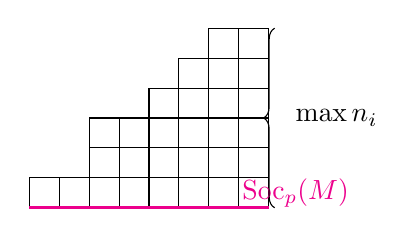
\begin{tikzpicture}[scale=0.38]
        \foreach \x/\h in {0/1,1/1,2/3,3/3,4/4,5/5,6/6,7/6} {
            \foreach \y in {1,...,\h} {
                \draw (\x,\y-1) rectangle (\x+1,\y);
            }
        }
        \draw[very thick, magenta] (0,0) -- (8,0);
        \node[magenta] at (8.9,0.5) {\(\operatorname{Soc}_p(M)\)};
        \draw[decorate, decoration={brace, amplitude=4pt}]
            (8.2,0) -- (8.2,6)
            node[midway, right=4pt] {\(\max n_i\)};
    \end{tikzpicture}
\]

Dopo il quoziente per il socle si ottiene il diagramma con una riga in meno:

\[
    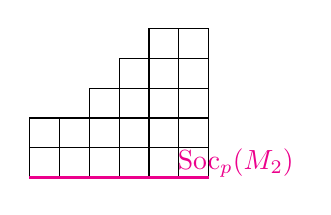
\begin{tikzpicture}[scale=0.38]
        \foreach \x/\h in {2/2,3/2,4/3,5/4,6/5,7/5} {
            \foreach \y in {1,...,\h} {
                \draw (\x,\y-1) rectangle (\x+1,\y);
            }
        }
        \draw[very thick, magenta] (2,0) -- (8,0);
        \node[magenta] at (8.9,0.5) {\(\operatorname{Soc}_p(M_2)\)};
    \end{tikzpicture}
\]

Continuando in questo modo si leggono le altezze delle colonne, cioè gli esponenti \(n_i\).

\section{Moduli liberi su domini a ideali principali}

\begin{snippetdefinition}{Lunghezza di un elemento}
    Sia \(A\) un dominio a ideali principali, e sia
    \[
        a\in A,
        \qquad
        a\neq 0.
    \]
    Scriviamo una fattorizzazione di \(a\) in elementi primi:
    \[
        a=u p_1^{n_1}\cdots p_r^{n_r},
        \qquad
        u\in A^\ast.
    \]
    Definiamo la lunghezza di \(a\) come
    \[
        \ell(a)=n_1+\cdots+n_r.
    \]
\end{snippetdefinition}

La lunghezza non dipende dalla specifica fattorizzazione scelta, per l'unicità della fattorizzazione in un dominio a fattorizzazione unica.

\begin{snippetremark}{}
    Se
    \[
        b\mid a,
    \]
    allora
    \[
        \ell(b)\leq \ell(a).
    \]
    Infatti ogni fattore primo che compare in \(b\) compare in \(a\) con esponente almeno altrettanto grande.
\end{snippetremark}

\begin{snippetremark}{Rango di un modulo libero finito}
    Se \(M\) è un \(A\)-modulo libero finitamente generato, allora
    \[
        M\simeq A^r
    \]
    per un certo \(r\geq 0\). Il numero \(r\) si chiama rango di \(M\), e coincide con il numero di elementi di una base di \(M\).
\end{snippetremark}

\begin{snippetlemma}{Separazione tramite un morfismo verso \(A\)}
    Sia
    \[
        \varphi\colon M\to A
    \]
    un morfismo di \(A\)-moduli. Supponiamo che esista \(v\in M\) tale che
    \[
        \operatorname{Im}(\varphi)=(\varphi(v)),
        \qquad
        \varphi(v)\neq 0.
    \]
    Allora
    \[
        M=Av\oplus\ker(\varphi).
    \]
\end{snippetlemma}

\begin{snippetproof}{}
    Poiché \(A\) è un dominio a ideali principali, l'immagine di \(\varphi\) è un ideale principale:
    \[
        \operatorname{Im}(\varphi)=(b),
        \qquad
        b=\varphi(v)\neq 0.
    \]

    Mostriamo che
    \[
        Av\intersection \ker(\varphi)=\{0_M\}.
    \]
    Sia
    \[
        w\in Av\intersection \ker(\varphi).
    \]
    Allora \(w=av\) per qualche \(a\in A\), e
    \[
        0_A=\varphi(w)=\varphi(av)=a\varphi(v)=ab.
    \]
    Poiché \(A\) è un dominio di integrità e \(b\neq 0\), segue
    \[
        a=0.
    \]
    Quindi
    \[
        w=0_M.
    \]

    Resta da mostrare che ogni elemento di \(M\) è somma di un elemento di \(Av\) e di un elemento di \(\ker(\varphi)\).

    Sia \(w\in M\). Poiché
    \[
        \varphi(w)\in\operatorname{Im}(\varphi)=(b),
    \]
    esiste \(c\in A\) tale che
    \[
        \varphi(w)=cb.
    \]
    Ma
    \[
        \varphi(cv)=c\varphi(v)=cb.
    \]
    Quindi
    \[
        \varphi(w-cv)=0_A,
    \]
    cioè
    \[
        w-cv\in\ker(\varphi).
    \]
    Pertanto
    \[
        w=cv+(w-cv)\in Av+\ker(\varphi).
    \]

    Concludiamo che
    \[
        M=Av\oplus\ker(\varphi).
    \]
\end{snippetproof}

\pagebreak
\part{Lezione 18}

\begin{snippetlemma}{Richiamo}
    Sia \(A\) un dominio a ideali principali e sia
    \[
        \varphi\colon M\to A
    \]
    un morfismo di \(A\)-moduli. Supponiamo che esista \(v\in M\) tale che
    \[
        \operatorname{Im}(\varphi)=(\varphi(v)),
        \qquad
        \varphi(v)\neq 0.
    \]
    Allora
    \[
        M=Av\oplus \ker(\varphi).
    \]
\end{snippetlemma}

\begin{snippettheorem}{Sottomoduli di moduli liberi su un DIP}
    Sia \(A\) un dominio a ideali principali.
    Sia \(M\) un \(A\)-modulo libero di rango finito
    \[
        \operatorname{rk}(M)=r.
    \]
    Se
    \[
        V\leq M
    \]
    è un \(A\)-sottomodulo, allora \(V\) è libero e
    \[
        \operatorname{rk}(V)\leq r.
    \]
\end{snippettheorem}

\begin{snippetproof}{}
    Procediamo per induzione su \(r=\operatorname{rk}(M)\).

    Se \(r=0\), allora \(M=\{0_M\}\), quindi anche \(V=\{0_M\}\), che è libero di rango \(0\).

    Supponiamo \(r=1\). Allora
    \[
        M=Av
    \]
    per qualche \(v\in M\), e \(M\simeq A\). Ogni sottomodulo \(V\leq M\) corrisponde quindi a un ideale \(I\triangleleft A\). Poiché \(A\) è un dominio a ideali principali,
    \[
        I=(c)
    \]
    per qualche \(c\in A\).

    Se \(c=0\), allora \(I=(0)\), dunque \(V=\{0_M\}\) è libero di rango \(0\). Se invece \(c\neq 0\), allora
    \[
        I=(c)\simeq A
    \]
    come \(A\)-modulo, tramite la mappa
    \[
        A\to (c),
        \qquad
        a\mapsto ac.
    \]
    Questa mappa è iniettiva perché \(A\) è un dominio di integrità. Quindi \(V\) è libero di rango \(1\).

    Supponiamo ora \(r>1\) e assumiamo la tesi vera per i moduli liberi di rango minore di \(r\).
    Scriviamo
    \[
        M\simeq A^r=A^{r-1}\oplus A.
    \]
    Poniamo
    \[
        W=A^{r-1}\oplus \{0\}\leq M.
    \]
    Allora \(W\) è libero di rango \(r-1\).

    Consideriamo
    \[
        V\intersection W\leq W.
    \]
    Per ipotesi induttiva,
    \[
        V\intersection W
    \]
    è libero e
    \[
        \operatorname{rk}(V\intersection W)\leq r-1.
    \]

    Se \(V\subseteq W\), allora \(V=V\intersection W\), e abbiamo concluso.

    Supponiamo quindi \(V\nsubseteq W\). Sia
    \[
        \pi\colon M=A^{r-1}\oplus A\to A
    \]
    la proiezione sull'ultima coordinata. Allora la restrizione
    \[
        \pi_{|V}\colon V\to A
    \]
    ha immagine non nulla, perché \(V\nsubseteq W=\ker(\pi)\).

    Siccome \(A\) è un dominio a ideali principali,
    \[
        \operatorname{Im}(\pi_{|V})=(c)
    \]
    per qualche \(c\neq 0\). Scegliamo \(v\in V\) tale che
    \[
        \pi(v)=c.
    \]
    Applicando il lemma precedente al morfismo
    \[
        \pi_{|V}\colon V\to A,
    \]
    otteniamo
    \[
        V=Av\oplus \ker(\pi_{|V}).
    \]
    Ma
    \[
        \ker(\pi_{|V})=V\intersection \ker(\pi)=V\intersection W.
    \]
    Quindi
    \[
        V=Av\oplus (V\intersection W).
    \]
    Poiché \(V\intersection W\) è libero di rango al più \(r-1\), segue che \(V\) è libero di rango al più \(r\).
\end{snippetproof}

\begin{snippetlemma}{MCD dei coefficienti e morfismi verso \(A\)}
    Sia \(M\) un \(A\)-modulo libero con base
    \[
        \mathcal{X}=\{v_1,\ldots,v_r\}.
    \]
    Sia
    \[
        w=a_1v_1+\cdots+a_rv_r\in M,
        \qquad
        a_i\in A.
    \]
    Sia
    \[
        b=\operatorname{MCD}(a_1,\ldots,a_r),
    \]
    cioè un generatore dell'ideale
    \[
        (a_1,\ldots,a_r)\triangleleft A.
    \]
    Allora:
    \begin{enumerate}
        \item per ogni morfismo di \(A\)-moduli
        \[
            \varphi\colon M\to A,
        \]
        si ha
        \[
            b\mid \varphi(w);
        \]

        \item esiste un morfismo di \(A\)-moduli
        \[
            \psi\colon M\to A
        \]
        tale che
        \[
            \psi(w)=b.
        \]
    \end{enumerate}
\end{snippetlemma}

\begin{snippetproof}{}
    Per il primo punto, se
    \[
        \varphi\colon M\to A
    \]
    è \(A\)-lineare, allora
    \[
        \varphi(w)
        =
        \varphi(a_1v_1+\cdots+a_rv_r)
        =
        a_1\varphi(v_1)+\cdots+a_r\varphi(v_r).
    \]
    Poiché \(b\) divide ciascun coefficiente \(a_i\), segue che \(b\mid \varphi(w)\).

    Per il secondo punto, siccome
    \[
        b=\operatorname{MCD}(a_1,\ldots,a_r),
    \]
    l'ideale generato da \(a_1,\ldots,a_r\) coincide con \((b)\). Quindi esistono
    \[
        c_1,\ldots,c_r\in A
    \]
    tali che
    \[
        b=a_1c_1+\cdots+a_rc_r.
    \]
    Per la proprietà universale dei moduli liberi, esiste un unico morfismo
    \[
        \psi\colon M\to A
    \]
    tale che
    \[
        \psi(v_i)=c_i
        \qquad
        \forall i=1,\ldots,r.
    \]
    Allora
    \[
        \psi(w)
        =
        a_1c_1+\cdots+a_rc_r
        =
        b.
    \]
\end{snippetproof}

\begin{snippetremark}{}
    Nel lemma precedente, il massimo comun divisore è inteso a meno di moltiplicazione per unità. Equivalentemente,
    \[
        \operatorname{MCD}(a_1,\ldots,a_r)
    \]
    è un generatore dell'ideale
    \[
        (a_1,\ldots,a_r).
    \]
\end{snippetremark}

\begin{snippetproposition}{Forma diagonale per sottomoduli di moduli liberi}
    Sia \(A\) un dominio a ideali principali e sia \(M\) un \(A\)-modulo libero di rango
    \[
        \operatorname{rk}(M)=r.
    \]
    Se
    \[
        V\leq M
    \]
    è un sottomodulo, allora esistono una base
    \[
        \mathcal{X}=\{x_1,\ldots,x_r\}
    \]
    di \(M\) e elementi
    \[
        c_1,\ldots,c_r\in A
    \]
    tali che
    \[
        V=\langle c_1x_1,\ldots,c_rx_r\rangle.
    \]
    In particolare, dopo aver eliminato i generatori nulli, \(V\) è libero.
\end{snippetproposition}

\begin{snippetproof}{}
    Procediamo per induzione su \(r=\operatorname{rk}(M)\).

    Se \(r=0\), allora \(M=0\) e la tesi è ovvia.

    Se \(r=1\), allora
    \[
        M=Ax
    \]
    per qualche \(x\). Un sottomodulo \(V\leq M\) corrisponde a un ideale \(I\triangleleft A\). Poiché \(A\) è un dominio a ideali principali,
    \[
        I=(c)
    \]
    per qualche \(c\in A\). Quindi
    \[
        V=A(cx),
    \]
    come richiesto.

    Supponiamo ora \(r>1\) e assumiamo la tesi vera per i moduli liberi di rango minore di \(r\).

    Se \(V=\{0_M\}\), basta prendere
    \[
        c_1=\cdots=c_r=0.
    \]
    Supponiamo dunque \(V\neq \{0_M\}\).

    Fissiamo una base iniziale
    \[
        \mathcal{Y}=\{y_1,\ldots,y_r\}
    \]
    di \(M\). Per ogni elemento non nullo
    \[
        w=a_1y_1+\cdots+a_ry_r\in V
    \]
    consideriamo
    \[
        d(w)=\operatorname{MCD}(a_1,\ldots,a_r).
    \]
    Scegliamo \(w\in V\setminus\{0_M\}\) in modo che la lunghezza
    \[
        \ell(d(w))
    \]
    sia minima.

    Scriviamo
    \[
        w=a_1y_1+\cdots+a_ry_r,
        \qquad
        d=d(w).
    \]
    Poiché \(d\mid a_i\) per ogni \(i\), possiamo scrivere
    \[
        a_i=da_i'
        \qquad
        \forall i.
    \]
    Poniamo
    \[
        x_1=a_1'y_1+\cdots+a_r'y_r.
    \]
    Allora
    \[
        w=dx_1,
    \]
    e
    \[
        \operatorname{MCD}(a_1',\ldots,a_r')=1.
    \]
    Per il lemma precedente esiste un morfismo
    \[
        \psi\colon M\to A
    \]
    tale che
    \[
        \psi(x_1)=1.
    \]
    In particolare,
    \[
        \operatorname{Im}(\psi)=A.
    \]
    Applicando il lemma di decomposizione a \(\psi\), otteniamo
    \[
        M=Ax_1\oplus \ker(\psi).
    \]
    Quindi \(\ker(\psi)\) è libero di rango \(r-1\).

    Consideriamo ora la restrizione
    \[
        \psi_{|V}\colon V\to A.
    \]
    Poiché
    \[
        \psi(w)=\psi(dx_1)=d,
    \]
    l'immagine \(\operatorname{Im}(\psi_{|V})\) contiene \(d\).
    Scriviamo
    \[
        \operatorname{Im}(\psi_{|V})=(c).
    \]
    Siccome \(d\in(c)\), abbiamo
    \[
        c\mid d.
    \]

    D'altra parte, \(c\in\operatorname{Im}(\psi_{|V})\), quindi esiste \(u\in V\) tale che
    \[
        \psi(u)=c.
    \]
    Se
    \[
        u=b_1y_1+\cdots+b_ry_r,
    \]
    poniamo
    \[
        d(u)=\operatorname{MCD}(b_1,\ldots,b_r).
    \]
    Per la scelta di \(w\), si ha
    \[
        \ell(d)\leq \ell(d(u)).
    \]
    Inoltre, per il lemma precedente applicato a \(u\) e al morfismo \(\psi\),
    \[
        d(u)\mid \psi(u)=c.
    \]
    Quindi
    \[
        \ell(d)\leq \ell(d(u))\leq \ell(c)\leq \ell(d).
    \]
    Tutte le disuguaglianze sono uguaglianze, dunque \(c\) e \(d\) sono associati. Pertanto
    \[
        \operatorname{Im}(\psi_{|V})=(d)=(\psi(w)).
    \]

    Applicando di nuovo il lemma di decomposizione, questa volta a
    \[
        \psi_{|V}\colon V\to A,
    \]
    otteniamo
    \[
        V=Aw\oplus \ker(\psi_{|V}).
    \]
    Ma
    \[
        \ker(\psi_{|V})=V\intersection \ker(\psi).
    \]
    Per ipotesi induttiva applicata al modulo libero \(\ker(\psi)\), esistono una base
    \[
        \{x_2,\ldots,x_r\}
    \]
    di \(\ker(\psi)\) e elementi
    \[
        c_2,\ldots,c_r\in A
    \]
    tali che
    \[
        V\intersection \ker(\psi)
        =
        \langle c_2x_2,\ldots,c_rx_r\rangle.
    \]
    Ponendo
    \[
        c_1=d,
    \]
    abbiamo
    \[
        w=dx_1=c_1x_1,
    \]
    e quindi
    \[
        V=\langle c_1x_1,c_2x_2,\ldots,c_rx_r\rangle.
    \]
    Inoltre
    \[
        M=Ax_1\oplus \ker(\psi),
    \]
    e \(\{x_2,\ldots,x_r\}\) è una base di \(\ker(\psi)\). Dunque
    \[
        \{x_1,\ldots,x_r\}
    \]
    è una base di \(M\), come volevamo.
\end{snippetproof}

\begin{snippetcorollary}{Indice di un sottomodulo di rango pieno}
    Sia \(M\) uno \(\mathbb{Z}\)-modulo libero di rango finito e sia
    \[
        V\leq M
    \]
    un sottomodulo tale che
    \[
        \operatorname{rk}(V)=\operatorname{rk}(M)=r.
    \]
    Sia
    \[
        \mathcal{X}=\{x_1,\ldots,x_r\}
    \]
    una base di \(M\) e sia
    \[
        \mathcal{Y}=\{y_1,\ldots,y_r\}
    \]
    una base di \(V\). Se \(C\in\operatorname{Mat}_r(\mathbb{Z})\) è la matrice del cambio di base che esprime i vettori di \(\mathcal{Y}\) in funzione di quelli di \(\mathcal{X}\), allora
    \[
        [M:V]=|\det(C)|.
    \]
\end{snippetcorollary}

\begin{snippetproof}{}
    Per la forma diagonale precedente, esiste una base
    \[
        \{x_1,\ldots,x_r\}
    \]
    di \(M\) e interi non nulli
    \[
        c_1,\ldots,c_r\in\mathbb{Z}
    \]
    tali che
    \[
        V=\langle c_1x_1,\ldots,c_rx_r\rangle.
    \]
    In questa base,
    \[
        M/V
        \simeq
        \mathbb{Z}/(c_1)\oplus\cdots\oplus \mathbb{Z}/(c_r).
    \]
    Quindi
    \[
        [M:V]
        =
        |M/V|
        =
        |c_1\cdots c_r|.
    \]
    D'altra parte, nella base diagonale la matrice di inclusione di \(V\) in \(M\) è
    \[
        \begin{pmatrix}
            c_1 & 0 & \cdots & 0\\
            0 & c_2 & \cdots & 0\\
            \vdots & \vdots & \ddots & \vdots\\
            0 & 0 & \cdots & c_r
        \end{pmatrix},
    \]
    il cui determinante ha valore assoluto
    \[
        |c_1\cdots c_r|.
    \]
    Cambiare basi in \(M\) e in \(V\) moltiplica la matrice a destra e a sinistra per matrici unimodulari, cioè con determinante \(\pm 1\). Perciò il valore assoluto del determinante non cambia.

    Dunque, per qualunque scelta di basi,
    \[
        [M:V]=|\det(C)|.
    \]
\end{snippetproof}

\section{Classificazione dei moduli finitamente generati su un DIP}

\begin{snippettheorem}{Classificazione}
    Sia \(A\) un dominio a ideali principali e sia \(M\) un \(A\)-modulo finitamente generato.
    Allora esistono
    \[
        r,s\in\naturalnumbers
    \]
    e elementi non nulli non invertibili
    \[
        c_1,\ldots,c_s\in A
    \]
    tali che
    \[
        M\simeq A^r\oplus A/(c_1)\oplus\cdots\oplus A/(c_s).
    \]
    Inoltre
    \[
        M/\operatorname{Tor}(M)\simeq A^r
    \]
    e
    \[
        \operatorname{Tor}(M)\simeq A/(c_1)\oplus\cdots\oplus A/(c_s).
    \]
\end{snippettheorem}

\begin{snippetproof}{}
    Poiché \(M\) è finitamente generato, esistono generatori
    \[
        v_1,\ldots,v_n\in M.
    \]
    Consideriamo il modulo libero
    \[
        A^n
    \]
    con base canonica
    \[
        e_1,\ldots,e_n.
    \]
    Per la proprietà universale dei moduli liberi, esiste un morfismo suriettivo
    \[
        \varphi\colon A^n\to M
    \]
    tale che
    \[
        \varphi(e_i)=v_i
        \qquad
        \forall i.
    \]
    Quindi, per il primo teorema di isomorfismo,
    \[
        M\simeq A^n/\ker(\varphi).
    \]

    Applichiamo la forma diagonale al sottomodulo
    \[
        \ker(\varphi)\leq A^n.
    \]
    Esiste una base
    \[
        x_1,\ldots,x_n
    \]
    di \(A^n\) ed esistono
    \[
        c_1,\ldots,c_n\in A
    \]
    tali che
    \[
        \ker(\varphi)
        =
        \langle c_1x_1,\ldots,c_nx_n\rangle.
    \]
    Allora
    \[
        A^n/\ker(\varphi)
        \simeq
        A/(c_1)\oplus\cdots\oplus A/(c_n).
    \]

    Ora distinguiamo i casi:
    \begin{itemize}
        \item se \(c_i=0\), allora
        \[
            A/(c_i)=A/(0)\simeq A;
        \]
        \item se \(c_i\in A^\ast\), allora
        \[
            A/(c_i)=A/(1)\simeq 0;
        \]
        \item se \(c_i\neq 0\) e \(c_i\notin A^\ast\), allora \(A/(c_i)\) è un modulo di torsione.
    \end{itemize}
    Eliminando i fattori nulli e raccogliendo i fattori liberi, otteniamo
    \[
        M\simeq A^r\oplus A/(c_1)\oplus\cdots\oplus A/(c_s),
    \]
    dove i \(c_i\) rimasti sono non nulli e non invertibili.

    Poiché \(A^r\) è privo di torsione e ciascun \(A/(c_i)\), con \(c_i\neq 0\), è di torsione, segue che
    \[
        \operatorname{Tor}(M)\simeq A/(c_1)\oplus\cdots\oplus A/(c_s),
    \]
    e quindi
    \[
        M/\operatorname{Tor}(M)\simeq A^r.
    \]
\end{snippetproof}

\begin{snippetcorollary}{Moduli finitamente generati senza torsione}
    Sia \(A\) un dominio a ideali principali.
    Se \(M\) è un \(A\)-modulo finitamente generato e privo di torsione, allora \(M\) è libero.
\end{snippetcorollary}

\begin{snippetproof}{}
    Per il teorema di classificazione,
    \[
        M\simeq A^r\oplus \operatorname{Tor}(M).
    \]
    Poiché \(M\) è privo di torsione,
    \[
        \operatorname{Tor}(M)=\{0_M\}.
    \]
    Quindi
    \[
        M\simeq A^r,
    \]
    e dunque \(M\) è libero.
\end{snippetproof}

\pagebreak
\part{Lezione 19}

\begin{snippetlemma}{Richiamo}
    Sia \(A\) un dominio a ideali principali e sia
    \[
        \varphi\colon M\to A
    \]
    un morfismo di \(A\)-moduli. Supponiamo che esista \(v\in M\) tale che
    \[
        \operatorname{Im}(\varphi)=(\varphi(v)),
        \qquad
        \varphi(v)\neq 0.
    \]
    Allora
    \[
        M=Av\oplus \ker(\varphi).
    \]
\end{snippetlemma}

\begin{snippettheorem}{Sottomoduli di moduli liberi su un DIP}
    Sia \(A\) un dominio a ideali principali.
    Sia \(M\) un \(A\)-modulo libero di rango finito
    \[
        \operatorname{rk}(M)=r.
    \]
    Se
    \[
        V\leq M
    \]
    è un \(A\)-sottomodulo, allora \(V\) è libero e
    \[
        \operatorname{rk}(V)\leq r.
    \]
\end{snippettheorem}

\begin{snippetproof}{}
    Procediamo per induzione su \(r=\operatorname{rk}(M)\).

    Se \(r=0\), allora \(M=\{0_M\}\), quindi anche \(V=\{0_M\}\), che è libero di rango \(0\).

    Supponiamo \(r=1\). Allora
    \[
        M=Av
    \]
    per qualche \(v\in M\), e \(M\simeq A\). Ogni sottomodulo \(V\leq M\) corrisponde quindi a un ideale \(I\triangleleft A\). Poiché \(A\) è un dominio a ideali principali,
    \[
        I=(c)
    \]
    per qualche \(c\in A\).

    Se \(c=0\), allora \(I=(0)\), dunque \(V=\{0_M\}\) è libero di rango \(0\). Se invece \(c\neq 0\), allora
    \[
        I=(c)\simeq A
    \]
    come \(A\)-modulo, tramite la mappa
    \[
        A\to (c),
        \qquad
        a\mapsto ac.
    \]
    Questa mappa è iniettiva perché \(A\) è un dominio di integrità. Quindi \(V\) è libero di rango \(1\).

    Supponiamo ora \(r>1\) e assumiamo la tesi vera per i moduli liberi di rango minore di \(r\).
    Scriviamo
    \[
        M\simeq A^r=A^{r-1}\oplus A.
    \]
    Poniamo
    \[
        W=A^{r-1}\oplus \{0\}\leq M.
    \]
    Allora \(W\) è libero di rango \(r-1\).

    Consideriamo
    \[
        V\intersection W\leq W.
    \]
    Per ipotesi induttiva,
    \[
        V\intersection W
    \]
    è libero e
    \[
        \operatorname{rk}(V\intersection W)\leq r-1.
    \]

    Se \(V\subseteq W\), allora \(V=V\intersection W\), e abbiamo concluso.

    Supponiamo quindi \(V\nsubseteq W\). Sia
    \[
        \pi\colon M=A^{r-1}\oplus A\to A
    \]
    la proiezione sull'ultima coordinata. Allora la restrizione
    \[
        \pi_{|V}\colon V\to A
    \]
    ha immagine non nulla, perché \(V\nsubseteq W=\ker(\pi)\).

    Siccome \(A\) è un dominio a ideali principali,
    \[
        \operatorname{Im}(\pi_{|V})=(c)
    \]
    per qualche \(c\neq 0\). Scegliamo \(v\in V\) tale che
    \[
        \pi(v)=c.
    \]
    Applicando il lemma precedente al morfismo
    \[
        \pi_{|V}\colon V\to A,
    \]
    otteniamo
    \[
        V=Av\oplus \ker(\pi_{|V}).
    \]
    Ma
    \[
        \ker(\pi_{|V})=V\intersection \ker(\pi)=V\intersection W.
    \]
    Quindi
    \[
        V=Av\oplus (V\intersection W).
    \]
    Poiché \(V\intersection W\) è libero di rango al più \(r-1\), segue che \(V\) è libero di rango al più \(r\).
\end{snippetproof}

\begin{snippetlemma}{MCD dei coefficienti e morfismi verso \(A\)}
    Sia \(M\) un \(A\)-modulo libero con base
    \[
        \mathcal{X}=\{v_1,\ldots,v_r\}.
    \]
    Sia
    \[
        w=a_1v_1+\cdots+a_rv_r\in M,
        \qquad
        a_i\in A.
    \]
    Sia
    \[
        b=\operatorname{MCD}(a_1,\ldots,a_r),
    \]
    cioè un generatore dell'ideale
    \[
        (a_1,\ldots,a_r)\triangleleft A.
    \]
    Allora:
    \begin{enumerate}
        \item per ogni morfismo di \(A\)-moduli
        \[
            \varphi\colon M\to A,
        \]
        si ha
        \[
            b\mid \varphi(w);
        \]

        \item esiste un morfismo di \(A\)-moduli
        \[
            \psi\colon M\to A
        \]
        tale che
        \[
            \psi(w)=b.
        \]
    \end{enumerate}
\end{snippetlemma}

\begin{snippetproof}{}
    Per il primo punto, se
    \[
        \varphi\colon M\to A
    \]
    è \(A\)-lineare, allora
    \[
        \varphi(w)
        =
        \varphi(a_1v_1+\cdots+a_rv_r)
        =
        a_1\varphi(v_1)+\cdots+a_r\varphi(v_r).
    \]
    Poiché \(b\) divide ciascun coefficiente \(a_i\), segue che \(b\mid \varphi(w)\).

    Per il secondo punto, siccome
    \[
        b=\operatorname{MCD}(a_1,\ldots,a_r),
    \]
    l'ideale generato da \(a_1,\ldots,a_r\) coincide con \((b)\). Quindi esistono
    \[
        c_1,\ldots,c_r\in A
    \]
    tali che
    \[
        b=a_1c_1+\cdots+a_rc_r.
    \]
    Per la proprietà universale dei moduli liberi, esiste un unico morfismo
    \[
        \psi\colon M\to A
    \]
    tale che
    \[
        \psi(v_i)=c_i
        \qquad
        \forall i=1,\ldots,r.
    \]
    Allora
    \[
        \psi(w)
        =
        a_1c_1+\cdots+a_rc_r
        =
        b.
    \]
\end{snippetproof}

\begin{snippetremark}{}
    Nel lemma precedente, il massimo comun divisore è inteso a meno di moltiplicazione per unità. Equivalentemente,
    \[
        \operatorname{MCD}(a_1,\ldots,a_r)
    \]
    è un generatore dell'ideale
    \[
        (a_1,\ldots,a_r).
    \]
\end{snippetremark}

\begin{snippetproposition}{Forma diagonale per sottomoduli di moduli liberi}
    Sia \(A\) un dominio a ideali principali e sia \(M\) un \(A\)-modulo libero di rango
    \[
        \operatorname{rk}(M)=r.
    \]
    Se
    \[
        V\leq M
    \]
    è un sottomodulo, allora esistono una base
    \[
        \mathcal{X}=\{x_1,\ldots,x_r\}
    \]
    di \(M\) e elementi
    \[
        c_1,\ldots,c_r\in A
    \]
    tali che
    \[
        V=\langle c_1x_1,\ldots,c_rx_r\rangle.
    \]
    In particolare, dopo aver eliminato i generatori nulli, \(V\) è libero.
\end{snippetproposition}

\begin{snippetproof}{}
    Procediamo per induzione su \(r=\operatorname{rk}(M)\).

    Se \(r=0\), allora \(M=0\) e la tesi è ovvia.

    Se \(r=1\), allora
    \[
        M=Ax
    \]
    per qualche \(x\). Un sottomodulo \(V\leq M\) corrisponde a un ideale \(I\triangleleft A\). Poiché \(A\) è un dominio a ideali principali,
    \[
        I=(c)
    \]
    per qualche \(c\in A\). Quindi
    \[
        V=A(cx),
    \]
    come richiesto.

    Supponiamo ora \(r>1\) e assumiamo la tesi vera per i moduli liberi di rango minore di \(r\).

    Se \(V=\{0_M\}\), basta prendere
    \[
        c_1=\cdots=c_r=0.
    \]
    Supponiamo dunque \(V\neq \{0_M\}\).

    Fissiamo una base iniziale
    \[
        \mathcal{Y}=\{y_1,\ldots,y_r\}
    \]
    di \(M\). Per ogni elemento non nullo
    \[
        w=a_1y_1+\cdots+a_ry_r\in V
    \]
    consideriamo
    \[
        d(w)=\operatorname{MCD}(a_1,\ldots,a_r).
    \]
    Scegliamo \(w\in V\setminus\{0_M\}\) in modo che la lunghezza
    \[
        \ell(d(w))
    \]
    sia minima.

    Scriviamo
    \[
        w=a_1y_1+\cdots+a_ry_r,
        \qquad
        d=d(w).
    \]
    Poiché \(d\mid a_i\) per ogni \(i\), possiamo scrivere
    \[
        a_i=da_i'
        \qquad
        \forall i.
    \]
    Poniamo
    \[
        x_1=a_1'y_1+\cdots+a_r'y_r.
    \]
    Allora
    \[
        w=dx_1,
    \]
    e
    \[
        \operatorname{MCD}(a_1',\ldots,a_r')=1.
    \]
    Per il lemma precedente esiste un morfismo
    \[
        \psi\colon M\to A
    \]
    tale che
    \[
        \psi(x_1)=1.
    \]
    In particolare,
    \[
        \operatorname{Im}(\psi)=A.
    \]
    Applicando il lemma di decomposizione a \(\psi\), otteniamo
    \[
        M=Ax_1\oplus \ker(\psi).
    \]
    Quindi \(\ker(\psi)\) è libero di rango \(r-1\).

    Consideriamo ora la restrizione
    \[
        \psi_{|V}\colon V\to A.
    \]
    Poiché
    \[
        \psi(w)=\psi(dx_1)=d,
    \]
    l'immagine \(\operatorname{Im}(\psi_{|V})\) contiene \(d\).
    Scriviamo
    \[
        \operatorname{Im}(\psi_{|V})=(c).
    \]
    Siccome \(d\in(c)\), abbiamo
    \[
        c\mid d.
    \]

    D'altra parte, \(c\in\operatorname{Im}(\psi_{|V})\), quindi esiste \(u\in V\) tale che
    \[
        \psi(u)=c.
    \]
    Se
    \[
        u=b_1y_1+\cdots+b_ry_r,
    \]
    poniamo
    \[
        d(u)=\operatorname{MCD}(b_1,\ldots,b_r).
    \]
    Per la scelta di \(w\), si ha
    \[
        \ell(d)\leq \ell(d(u)).
    \]
    Inoltre, per il lemma precedente applicato a \(u\) e al morfismo \(\psi\),
    \[
        d(u)\mid \psi(u)=c.
    \]
    Quindi
    \[
        \ell(d)\leq \ell(d(u))\leq \ell(c)\leq \ell(d).
    \]
    Tutte le disuguaglianze sono uguaglianze, dunque \(c\) e \(d\) sono associati. Pertanto
    \[
        \operatorname{Im}(\psi_{|V})=(d)=(\psi(w)).
    \]

    Applicando di nuovo il lemma di decomposizione, questa volta a
    \[
        \psi_{|V}\colon V\to A,
    \]
    otteniamo
    \[
        V=Aw\oplus \ker(\psi_{|V}).
    \]
    Ma
    \[
        \ker(\psi_{|V})=V\intersection \ker(\psi).
    \]
    Per ipotesi induttiva applicata al modulo libero \(\ker(\psi)\), esistono una base
    \[
        \{x_2,\ldots,x_r\}
    \]
    di \(\ker(\psi)\) e elementi
    \[
        c_2,\ldots,c_r\in A
    \]
    tali che
    \[
        V\intersection \ker(\psi)
        =
        \langle c_2x_2,\ldots,c_rx_r\rangle.
    \]
    Ponendo
    \[
        c_1=d,
    \]
    abbiamo
    \[
        w=dx_1=c_1x_1,
    \]
    e quindi
    \[
        V=\langle c_1x_1,c_2x_2,\ldots,c_rx_r\rangle.
    \]
    Inoltre
    \[
        M=Ax_1\oplus \ker(\psi),
    \]
    e \(\{x_2,\ldots,x_r\}\) è una base di \(\ker(\psi)\). Dunque
    \[
        \{x_1,\ldots,x_r\}
    \]
    è una base di \(M\), come volevamo.
\end{snippetproof}

\begin{snippetcorollary}{Indice di un sottomodulo di rango pieno}
    Sia \(M\) uno \(\mathbb{Z}\)-modulo libero di rango finito e sia
    \[
        V\leq M
    \]
    un sottomodulo tale che
    \[
        \operatorname{rk}(V)=\operatorname{rk}(M)=r.
    \]
    Sia
    \[
        \mathcal{X}=\{x_1,\ldots,x_r\}
    \]
    una base di \(M\) e sia
    \[
        \mathcal{Y}=\{y_1,\ldots,y_r\}
    \]
    una base di \(V\). Se \(C\in\operatorname{Mat}_r(\mathbb{Z})\) è la matrice del cambio di base che esprime i vettori di \(\mathcal{Y}\) in funzione di quelli di \(\mathcal{X}\), allora
    \[
        [M:V]=|\det(C)|.
    \]
\end{snippetcorollary}

\begin{snippetproof}{}
    Per la forma diagonale precedente, esiste una base
    \[
        \{x_1,\ldots,x_r\}
    \]
    di \(M\) e interi non nulli
    \[
        c_1,\ldots,c_r\in\mathbb{Z}
    \]
    tali che
    \[
        V=\langle c_1x_1,\ldots,c_rx_r\rangle.
    \]
    In questa base,
    \[
        M/V
        \simeq
        \mathbb{Z}/(c_1)\oplus\cdots\oplus \mathbb{Z}/(c_r).
    \]
    Quindi
    \[
        [M:V]
        =
        |M/V|
        =
        |c_1\cdots c_r|.
    \]
    D'altra parte, nella base diagonale la matrice di inclusione di \(V\) in \(M\) è
    \[
        \begin{pmatrix}
            c_1 & 0 & \cdots & 0\\
            0 & c_2 & \cdots & 0\\
            \vdots & \vdots & \ddots & \vdots\\
            0 & 0 & \cdots & c_r
        \end{pmatrix},
    \]
    il cui determinante ha valore assoluto
    \[
        |c_1\cdots c_r|.
    \]
    Cambiare basi in \(M\) e in \(V\) moltiplica la matrice a destra e a sinistra per matrici unimodulari, cioè con determinante \(\pm 1\). Perciò il valore assoluto del determinante non cambia.

    Dunque, per qualunque scelta di basi,
    \[
        [M:V]=|\det(C)|.
    \]
\end{snippetproof}

\section{Classificazione dei moduli finitamente generati su un DIP}

\begin{snippettheorem}{Classificazione}
    Sia \(A\) un dominio a ideali principali e sia \(M\) un \(A\)-modulo finitamente generato.
    Allora esistono
    \[
        r,s\in\naturalnumbers
    \]
    e elementi non nulli non invertibili
    \[
        c_1,\ldots,c_s\in A
    \]
    tali che
    \[
        M\simeq A^r\oplus A/(c_1)\oplus\cdots\oplus A/(c_s).
    \]
    Inoltre
    \[
        M/\operatorname{Tor}(M)\simeq A^r
    \]
    e
    \[
        \operatorname{Tor}(M)\simeq A/(c_1)\oplus\cdots\oplus A/(c_s).
    \]
\end{snippettheorem}

\begin{snippetproof}{}
    Poiché \(M\) è finitamente generato, esistono generatori
    \[
        v_1,\ldots,v_n\in M.
    \]
    Consideriamo il modulo libero
    \[
        A^n
    \]
    con base canonica
    \[
        e_1,\ldots,e_n.
    \]
    Per la proprietà universale dei moduli liberi, esiste un morfismo suriettivo
    \[
        \varphi\colon A^n\to M
    \]
    tale che
    \[
        \varphi(e_i)=v_i
        \qquad
        \forall i.
    \]
    Quindi, per il primo teorema di isomorfismo,
    \[
        M\simeq A^n/\ker(\varphi).
    \]

    Applichiamo la forma diagonale al sottomodulo
    \[
        \ker(\varphi)\leq A^n.
    \]
    Esiste una base
    \[
        x_1,\ldots,x_n
    \]
    di \(A^n\) ed esistono
    \[
        c_1,\ldots,c_n\in A
    \]
    tali che
    \[
        \ker(\varphi)
        =
        \langle c_1x_1,\ldots,c_nx_n\rangle.
    \]
    Allora
    \[
        A^n/\ker(\varphi)
        \simeq
        A/(c_1)\oplus\cdots\oplus A/(c_n).
    \]

    Ora distinguiamo i casi:
    \begin{itemize}
        \item se \(c_i=0\), allora
        \[
            A/(c_i)=A/(0)\simeq A;
        \]
        \item se \(c_i\in A^\ast\), allora
        \[
            A/(c_i)=A/(1)\simeq 0;
        \]
        \item se \(c_i\neq 0\) e \(c_i\notin A^\ast\), allora \(A/(c_i)\) è un modulo di torsione.
    \end{itemize}
    Eliminando i fattori nulli e raccogliendo i fattori liberi, otteniamo
    \[
        M\simeq A^r\oplus A/(c_1)\oplus\cdots\oplus A/(c_s),
    \]
    dove i \(c_i\) rimasti sono non nulli e non invertibili.

    Poiché \(A^r\) è privo di torsione e ciascun \(A/(c_i)\), con \(c_i\neq 0\), è di torsione, segue che
    \[
        \operatorname{Tor}(M)\simeq A/(c_1)\oplus\cdots\oplus A/(c_s),
    \]
    e quindi
    \[
        M/\operatorname{Tor}(M)\simeq A^r.
    \]
\end{snippetproof}

\begin{snippetcorollary}{Moduli finitamente generati senza torsione}
    Sia \(A\) un dominio a ideali principali.
    Se \(M\) è un \(A\)-modulo finitamente generato e privo di torsione, allora \(M\) è libero.
\end{snippetcorollary}

\begin{snippetproof}{}
    Per il teorema di classificazione,
    \[
        M\simeq A^r\oplus \operatorname{Tor}(M).
    \]
    Poiché \(M\) è privo di torsione,
    \[
        \operatorname{Tor}(M)=\{0_M\}.
    \]
    Quindi
    \[
        M\simeq A^r,
    \]
    e dunque \(M\) è libero.
\end{snippetproof}

\pagebreak
\part{Lezione 20}

\subsection{Conclusione sulla classificazione dei gruppi abeliani finiti}

\begin{snippetcorollary}{Prodotto di due gruppi ciclici}
    Siano
    \[
        C_m\simeq \mathbb{Z}/m\mathbb{Z},
        \qquad
        C_n\simeq \mathbb{Z}/n\mathbb{Z}
    \]
    due gruppi ciclici finiti. Allora
    \[
        C_m\times C_n\simeq C_{mn}
        \iff
        \operatorname{MCD}(m,n)=1.
    \]
\end{snippetcorollary}

\begin{snippetproof}{}
    Scriviamo le fattorizzazioni in primi:
    \[
        m=p_1^{h_1}\cdots p_r^{h_r},
        \qquad
        n=q_1^{k_1}\cdots q_s^{k_s},
    \]
    con
    \[
        h_i,k_j\geq 1.
    \]

    Supponiamo prima che
    \[
        \operatorname{MCD}(m,n)=1.
    \]
    Allora nessun primo \(p_i\) coincide, a meno di associati in \(\mathbb{Z}\), con uno dei primi \(q_j\).
    Come \(\mathbb{Z}\)-moduli,
    \[
        C_m\times C_n
        \simeq
        \mathbb{Z}/m\mathbb{Z}\oplus \mathbb{Z}/n\mathbb{Z}.
    \]
    Per il teorema cinese del resto,
    \[
        \mathbb{Z}/m\mathbb{Z}\oplus \mathbb{Z}/n\mathbb{Z}
        \simeq
        \mathbb{Z}/mn\mathbb{Z},
    \]
    perché gli ideali \((m)\) e \((n)\) sono coprimi.
    Quindi
    \[
        C_m\times C_n\simeq C_{mn}.
    \]

    Viceversa, supponiamo
    \[
        \operatorname{MCD}(m,n)\neq 1.
    \]
    Allora esiste un primo \(p\) che divide sia \(m\) sia \(n\).
    Scriviamo
    \[
        m=p^h m',
        \qquad
        n=p^k n',
    \]
    con
    \[
        h,k\geq 1,
        \qquad
        p\nmid m',
        \qquad
        p\nmid n'.
    \]
    La componente \(p\)-primaria di
    \[
        C_m\times C_n
    \]
    contiene due fattori ciclici:
    \[
        \mathbb{Z}/p^h\mathbb{Z}
        \oplus
        \mathbb{Z}/p^k\mathbb{Z}.
    \]
    Invece la componente \(p\)-primaria di
    \[
        C_{mn}
        \simeq
        \mathbb{Z}/mn\mathbb{Z}
    \]
    è un solo fattore ciclico:
    \[
        \mathbb{Z}/p^{h+k}\mathbb{Z}.
    \]
    I diagrammi \(p\)-primari sono quindi diversi: nel primo caso ci sono due colonne, nel secondo una sola colonna. Per l'unicità della decomposizione dei gruppi abeliani finiti, i due gruppi non possono essere isomorfi.

    Dunque
    \[
        C_m\times C_n\simeq C_{mn}
        \iff
        \operatorname{MCD}(m,n)=1.
    \]
\end{snippetproof}

\begin{snippetremark}{Lettura tramite divisori elementari}
    Se
    \[
        \operatorname{MCD}(m,n)\neq 1,
    \]
    e i primi comuni sono
    \[
        p_1,\ldots,p_t,
    \]
    allora, scrivendo
    \[
        m=p_1^{h_1}\cdots p_t^{h_t}m',
        \qquad
        n=p_1^{k_1}\cdots p_t^{k_t}n',
    \]
    con \(p_i\nmid m'n'\), nella decomposizione di
    \[
        C_m\times C_n
    \]
    compaiono, per ogni \(p_i\), due colonne di altezze \(h_i\) e \(k_i\).
    I due divisori elementari corrispondenti sono ottenuti usando
    \[
        \min\{h_i,k_i\}
        \qquad
        \text{e}
        \qquad
        \max\{h_i,k_i\}.
    \]
    In particolare la successione dei divisori elementari è diversa da quella di \(C_{mn}\).
\end{snippetremark}

\section{Endomorfismi e moduli su \(K[X]\)}

D'ora in avanti sia \(K\) un campo e poniamo
\[
    A=K[X].
\]
Sia
\[
    V=K^n
\]
uno spazio vettoriale di dimensione finita su \(K\), e sia
\[
    \varphi\colon V\to V
\]
un endomorfismo \(K\)-lineare.

La scelta di una base di \(V\) associa a \(\varphi\) una matrice
\[
    B\in\operatorname{Mat}_n(K).
\]
Per ogni \(k\in\naturalnumbers\), indichiamo con
\[
    \varphi^k=\underbrace{\varphi\circ\cdots\circ\varphi}_{k\text{ volte}}
\]
la \(k\)-esima iterata di \(\varphi\), con la convenzione
\[
    \varphi^0=\operatorname{Id}_V.
\]

Vogliamo trasformare \(V\) in un \(K[X]\)-modulo usando l'endomorfismo \(\varphi\).

\begin{snippetdefinition}{Modulo associato a un endomorfismo}
    Definiamo un'azione di \(K[X]\) su \(V\) ponendo
    \[
        X\cdot v=\varphi(v)
        \qquad
        \forall v\in V,
    \]
    e quindi, per
    \[
        f=a_0+a_1X+\cdots+a_mX^m\in K[X],
    \]
    ponendo
    \[
        f\cdot v
        =
        a_0v+a_1\varphi(v)+\cdots+a_m\varphi^m(v).
    \]
    Con questa azione, \(V\) diventa un \(K[X]\)-modulo.
\end{snippetdefinition}

\begin{snippetproof}{}
    Le proprietà di modulo seguono dalla linearità di \(\varphi\) e dalle regole di composizione delle sue potenze.

    Infatti, per \(f,g\in K[X]\) e \(v\in V\),
    \[
        (f+g)\cdot v=f\cdot v+g\cdot v
    \]
    è immediato. Inoltre, se
    \[
        f=\sum_i a_iX^i,
        \qquad
        g=\sum_j b_jX^j,
    \]
    allora
    \begin{align*}
        (fg)\cdot v
        &=
        \left(\sum_{i,j}a_ib_jX^{i+j}\right)\cdot v \\
        &=
        \sum_{i,j}a_ib_j\varphi^{i+j}(v) \\
        &=
        \sum_i a_i\varphi^i\left(\sum_j b_j\varphi^j(v)\right) \\
        &=
        f\cdot(g\cdot v).
    \end{align*}
    Infine \(1\cdot v=v\).
\end{snippetproof}

\begin{snippetdefinition}{Sottospazio stabile}
    Un sottospazio vettoriale
    \[
        W\leq V
    \]
    si dice \(\varphi\)-stabile se
    \[
        \varphi(w)\in W
        \qquad
        \forall w\in W.
    \]
\end{snippetdefinition}

\begin{snippetproposition}{Sottospazi stabili e sottomoduli}
    Un sottospazio vettoriale \(W\leq V\) è \(\varphi\)-stabile se e solo se è un \(K[X]\)-sottomodulo di \(V\).
\end{snippetproposition}

\begin{snippetproof}{}
    Se \(W\) è un \(K[X]\)-sottomodulo, allora per ogni \(w\in W\)
    \[
        \varphi(w)=X\cdot w\in W,
    \]
    quindi \(W\) è \(\varphi\)-stabile.

    Viceversa, supponiamo che \(W\) sia \(\varphi\)-stabile. Allora, per induzione,
    \[
        \varphi^k(w)\in W
        \qquad
        \forall k\geq 0,\ \forall w\in W.
    \]
    Quindi, per ogni
    \[
        f=a_0+a_1X+\cdots+a_mX^m\in K[X],
    \]
    si ha
    \[
        f\cdot w
        =
        a_0w+a_1\varphi(w)+\cdots+a_m\varphi^m(w)\in W.
    \]
    Dunque \(W\) è un \(K[X]\)-sottomodulo.
\end{snippetproof}

\begin{snippetexample}{Matrici a blocchi e sottospazi stabili}
    Sia
    \[
        \mathcal{B}
        =
        \{w_1,\ldots,w_m,u_1,\ldots,u_s\}
    \]
    una base di \(V\), e poniamo
    \[
        W=\operatorname{Span}_K\{w_1,\ldots,w_m\},
        \qquad
        U=\operatorname{Span}_K\{u_1,\ldots,u_s\}.
    \]
    Allora
    \[
        V=W\oplus U
    \]
    come \(K\)-spazi vettoriali.

    Se la matrice di \(\varphi\) rispetto alla base \(\mathcal{B}\) ha la forma
    \[
        B=
        \begin{pmatrix}
            B_1 & B_2\\
            0 & B_3
        \end{pmatrix},
    \]
    allora \(W\) è \(\varphi\)-stabile. Infatti le immagini dei vettori \(w_1,\ldots,w_m\) sono combinazioni lineari dei soli \(w_i\).

    In generale, però, \(U\) non è \(\varphi\)-stabile: l'immagine di un vettore \(u_j\) può avere componenti lungo \(W\), descritte dal blocco \(B_2\).
\end{snippetexample}

\begin{snippetremark}{Decomposizioni stabili e matrici diagonali a blocchi}
    Supponiamo che
    \[
        V=W_1\oplus\cdots\oplus W_r
    \]
    con ciascun \(W_i\) \(\varphi\)-stabile.
    Scegliendo una base di ogni \(W_i\) e concatenandole, la matrice di \(\varphi\) è diagonale a blocchi:
    \[
        B=
        \begin{pmatrix}
            B_1 & 0 & \cdots & 0\\
            0 & B_2 & \cdots & 0\\
            \vdots & \vdots & \ddots & \vdots\\
            0 & 0 & \cdots & B_r
        \end{pmatrix},
    \]
    dove \(B_i\) rappresenta
    \[
        \varphi_{|W_i}\colon W_i\to W_i.
    \]
    In questo caso
    \[
        \det(B)=\det(B_1)\cdots\det(B_r)
    \]
    e
    \[
        \operatorname{rk}(B)
        =
        \operatorname{rk}(B_1)+\cdots+\operatorname{rk}(B_r).
    \]
\end{snippetremark}

\subsection{Il modulo associato è di torsione}

\begin{snippetproposition}{}
    Il \(K[X]\)-modulo \(V\) associato a \(\varphi\) è di torsione:
    \[
        V=\operatorname{Tor}(V).
    \]
\end{snippetproposition}

\begin{snippetproof}{}
    Sia
    \[
        v\in V,
        \qquad
        v\neq 0.
    \]
    Vogliamo mostrare che
    \[
        \operatorname{Ann}(v)\neq \{0\}.
    \]

    Consideriamo la successione di vettori
    \[
        v,\ \varphi(v),\ \varphi^2(v),\ldots.
    \]
    Poiché \(V\) ha dimensione finita, esiste \(m\geq 1\) tale che
    \[
        \{v,\varphi(v),\ldots,\varphi^m(v)\}
    \]
    sia linearmente dipendente.

    Scegliamo \(m\) minimo con questa proprietà. Allora
    \[
        \{v,\varphi(v),\ldots,\varphi^{m-1}(v)\}
    \]
    è linearmente indipendente, e quindi esiste una relazione
    \[
        a_0v+a_1\varphi(v)+\cdots+a_{m-1}\varphi^{m-1}(v)+a_m\varphi^m(v)=0,
    \]
    con coefficienti non tutti nulli.
    Per la minimalità di \(m\), necessariamente
    \[
        a_m\neq 0.
    \]
    Dividendo per \(a_m\), possiamo supporre
    \[
        a_m=1.
    \]
    Poniamo
    \[
        f_v
        =
        a_0+a_1X+\cdots+a_{m-1}X^{m-1}+X^m.
    \]
    Allora
    \[
        f_v\cdot v=0,
    \]
    quindi
    \[
        f_v\in\operatorname{Ann}(v),
        \qquad
        f_v\neq 0.
    \]
    Dunque \(v\) è di torsione.

    Poiché anche \(0_V\) è di torsione, concludiamo che
    \[
        V=\operatorname{Tor}(V).
    \]
\end{snippetproof}

\begin{snippetdefinition}{Sottospazio ciclico generato da un vettore}
    Per \(v\in V\), definiamo
    \[
        W(v)=K[X]v
        =
        \{f\cdot v\mid f\in K[X]\}.
    \]
    Questo è il \(K[X]\)-sottomodulo ciclico generato da \(v\), cioè il più piccolo sottospazio \(\varphi\)-stabile che contiene \(v\).
\end{snippetdefinition}

\begin{snippetproposition}{Annullatore e base del sottospazio ciclico}
    Sia \(v\in V\), \(v\neq 0\), e sia \(m\) minimo tale che
    \[
        \{v,\varphi(v),\ldots,\varphi^m(v)\}
    \]
    sia linearmente dipendente.
    Allora esiste un unico polinomio monico
    \[
        f_v=X^m+a_{m-1}X^{m-1}+\cdots+a_1X+a_0
    \]
    tale che
    \[
        f_v\cdot v=0.
    \]
    Inoltre
    \[
        \operatorname{Ann}(v)=(f_v)
    \]
    e
    \[
        W(v)=\operatorname{Span}_K\{v,\varphi(v),\ldots,\varphi^{m-1}(v)\}.
    \]
\end{snippetproposition}

\begin{snippetproof}{}
    L'esistenza di \(f_v\) è stata costruita nella dimostrazione precedente.

    Mostriamo che l'annullatore è proprio \((f_v)\).
    Poiché
    \[
        f_v\cdot v=0,
    \]
    abbiamo
    \[
        (f_v)\subseteq\operatorname{Ann}(v).
    \]

    Sia ora
    \[
        g\in\operatorname{Ann}(v).
    \]
    Dividiamo \(g\) per \(f_v\):
    \[
        g=qf_v+r,
        \qquad
        r=0
        \quad
        \text{oppure}
        \quad
        \deg(r)<m.
    \]
    Applicando a \(v\), otteniamo
    \[
        0=g\cdot v=q\cdot(f_v\cdot v)+r\cdot v=r\cdot v.
    \]
    Se \(r\neq 0\), allora \(r\cdot v\) è una combinazione lineare non banale di
    \[
        v,\varphi(v),\ldots,\varphi^{m-1}(v),
    \]
    contro la loro indipendenza lineare.
    Quindi \(r=0\), e dunque
    \[
        f_v\mid g.
    \]
    Pertanto
    \[
        \operatorname{Ann}(v)=(f_v).
    \]

    Infine, poiché
    \[
        X^m\cdot v
        =
        \varphi^m(v)
        =
        -a_{m-1}\varphi^{m-1}(v)-\cdots-a_1\varphi(v)-a_0v,
    \]
    ogni potenza successiva \(\varphi^k(v)\) si riduce a combinazione lineare di
    \[
        v,\varphi(v),\ldots,\varphi^{m-1}(v).
    \]
    Quindi
    \[
        W(v)=\operatorname{Span}_K\{v,\varphi(v),\ldots,\varphi^{m-1}(v)\}.
    \]
\end{snippetproof}

\begin{snippetcorollary}{}
    Con le notazioni precedenti,
    \[
        W(v)\simeq K[X]/(f_v)
    \]
    come \(K[X]\)-moduli.
\end{snippetcorollary}

\begin{snippetproof}{}
    Il modulo \(W(v)\) è ciclico generato da \(v\), e il suo annullatore è
    \[
        \operatorname{Ann}(v)=(f_v).
    \]
    Per il teorema sui moduli ciclici,
    \[
        W(v)\simeq K[X]/\operatorname{Ann}(v)=K[X]/(f_v).
    \]
\end{snippetproof}

\subsection{Matrice compagna}

Sia
\[
    f=X^m+a_{m-1}X^{m-1}+\cdots+a_1X+a_0\in K[X]
\]
un polinomio monico di grado \(m\geq 1\).

\begin{snippetdefinition}{Matrice compagna}
    La matrice compagna di \(f\) è
    \[
        C(f)
        =
        \begin{pmatrix}
            0 & 0 & \cdots & 0 & -a_0\\
            1 & 0 & \cdots & 0 & -a_1\\
            0 & 1 & \cdots & 0 & -a_2\\
            \vdots & \vdots & \ddots & \vdots & \vdots\\
            0 & 0 & \cdots & 1 & -a_{m-1}
        \end{pmatrix}.
    \]
\end{snippetdefinition}

\begin{snippetproposition}{Matrice del sottospazio ciclico}
    Sia \(v\in V\), \(v\neq 0\), e sia
    \[
        f_v=X^m+a_{m-1}X^{m-1}+\cdots+a_1X+a_0
    \]
    il generatore monico di \(\operatorname{Ann}(v)\).
    Rispetto alla base
    \[
        \mathcal{B}_v=
        \{v,\varphi(v),\ldots,\varphi^{m-1}(v)\}
    \]
    di \(W(v)\), la matrice di
    \[
        \varphi_{|W(v)}\colon W(v)\to W(v)
    \]
    è la matrice compagna
    \[
        C(f_v).
    \]
\end{snippetproposition}

\begin{snippetproof}{}
    Per \(i=0,\ldots,m-2\), si ha
    \[
        \varphi(\varphi^i(v))=\varphi^{i+1}(v),
    \]
    quindi le prime \(m-1\) colonne della matrice sono quelle con \(1\) sulla sottodiagonale e \(0\) altrove.

    Inoltre, dalla relazione
    \[
        f_v\cdot v=0
    \]
    otteniamo
    \[
        \varphi^m(v)
        =
        -a_0v-a_1\varphi(v)-\cdots-a_{m-1}\varphi^{m-1}(v).
    \]
    Questa è esattamente l'ultima colonna della matrice compagna.
    Quindi la matrice cercata è \(C(f_v)\).
\end{snippetproof}

\begin{snippetlemma}{Polinomio caratteristico della matrice compagna}
    Il polinomio caratteristico di \(C(f)\) è \(f\):
    \[
        \chi_{C(f)}(T)=\det(TI_m-C(f))=f(T).
    \]
\end{snippetlemma}

\begin{snippetproof}{}
    Per \(m=1\), abbiamo
    \[
        f=X+a_0,
        \qquad
        C(f)=(-a_0),
    \]
    quindi
    \[
        \chi_{C(f)}(T)=T+a_0=f(T).
    \]

    Supponiamo ora \(m\geq 2\). Allora
    \[
        TI_m-C(f)
        =
        \begin{pmatrix}
            T & 0 & \cdots & 0 & a_0\\
            -1 & T & \cdots & 0 & a_1\\
            0 & -1 & \ddots & 0 & a_2\\
            \vdots & \vdots & \ddots & T & \vdots\\
            0 & 0 & \cdots & -1 & T+a_{m-1}
        \end{pmatrix}.
    \]
    Sviluppando il determinante lungo la prima riga, o procedendo per induzione sulla dimensione, si ottiene
    \[
        \det(TI_m-C(f))
        =
        T^m+a_{m-1}T^{m-1}+\cdots+a_1T+a_0.
    \]
    Dunque
    \[
        \chi_{C(f)}(T)=f(T).
    \]
\end{snippetproof}

\begin{snippetremark}{Significato}
    Ogni sottospazio ciclico \(W(v)\) produce una base nella quale l'endomorfismo è rappresentato da una matrice compagna.
    La decomposizione di \(V\) come \(K[X]\)-modulo di torsione corrisponderà quindi a una decomposizione della matrice di \(\varphi\) in blocchi compagni.
\end{snippetremark}

\pagebreak
\part{Lezione 21}

\subsection{Forma canonica primaria e forma canonica razionale}

Sia \(V\) uno spazio vettoriale di dimensione finita su un campo \(K\), e sia
\[
    \varphi\colon V\to V
\]
un endomorfismo.

Come visto, \(V\) diventa un \(K[X]\)-modulo ponendo
\[
    X\cdot v=\varphi(v)
    \qquad
    \forall v\in V.
\]
Poiché \(\dim_K(V)<\infty\), questo \(K[X]\)-modulo è di torsione.

Se \(v\in V\), \(v\neq 0\), allora
\[
    W_v=K[X]v
\]
è un \(K[X]\)-modulo ciclico, e quindi
\[
    W_v\simeq K[X]/\operatorname{Ann}(v).
\]
Poiché \(K[X]\) è un dominio a ideali principali, esiste un unico polinomio monico \(f_v\in K[X]\) tale che
\[
    \operatorname{Ann}(v)=(f_v).
\]
Se
\[
    f_v=X^m+a_{m-1}X^{m-1}+\cdots+a_1X+a_0,
\]
allora \(W_v\) ammette una base rispetto alla quale \(\varphi_{|W_v}\) è rappresentata dalla matrice compagna
\[
    C(f_v)
    =
    \begin{pmatrix}
        0 & 0 & \cdots & 0 & -a_0\\
        1 & 0 & \cdots & 0 & -a_1\\
        0 & 1 & \cdots & 0 & -a_2\\
        \vdots & \vdots & \ddots & \vdots & \vdots\\
        0 & 0 & \cdots & 1 & -a_{m-1}
    \end{pmatrix}.
\]
Inoltre
\[
    \chi_{C(f_v)}(T)=f_v(T).
\]

\begin{snippettheorem}{Forma canonica primaria}
    Sia \(V\) uno spazio vettoriale di dimensione finita su \(K\), e sia
    \[
        \varphi\colon V\to V
    \]
    un endomorfismo.

    Allora esistono polinomi monici irriducibili
    \[
        f_1,\ldots,f_t\in K[X]
    \]
    ed esponenti
    \[
        n_1,\ldots,n_t\geq 1
    \]
    tali che esiste una base di \(V\) rispetto alla quale \(\varphi\) è rappresentata da una matrice diagonale a blocchi
    \[
        \begin{pmatrix}
            C(f_1^{n_1}) & 0 & \cdots & 0\\
            0 & C(f_2^{n_2}) & \cdots & 0\\
            \vdots & \vdots & \ddots & \vdots\\
            0 & 0 & \cdots & C(f_t^{n_t})
        \end{pmatrix}.
    \]
    I blocchi
    \[
        C(f_i^{n_i})
    \]
    sono univocamente determinati a meno dell'ordine.
\end{snippettheorem}

\begin{snippetproof}{}
    Poiché \(\dim_K(V)<\infty\), il modulo \(V\) è finitamente generato come \(K[X]\)-modulo. Inoltre abbiamo visto che
    \[
        V=\operatorname{Tor}(V).
    \]
    Applichiamo quindi la classificazione dei moduli finitamente generati di torsione su un dominio a ideali principali, con
    \[
        A=K[X].
    \]
    Otteniamo una decomposizione
    \[
        V\simeq
        K[X]/(f_1^{n_1})
        \oplus\cdots\oplus
        K[X]/(f_t^{n_t}),
    \]
    dove i \(f_i\) sono polinomi monici irriducibili e gli \(n_i\) sono interi positivi.

    Ogni summando
    \[
        K[X]/(f_i^{n_i})
    \]
    è ciclico. Sia \(v_i\) un generatore del corrispondente sottomodulo
    \[
        W_i\simeq K[X]/(f_i^{n_i}).
    \]
    Allora
    \[
        \operatorname{Ann}(v_i)=(f_i^{n_i}).
    \]
    Se
    \[
        m_i=\deg(f_i^{n_i}),
    \]
    il sottomodulo \(W_i\) ha una base
    \[
        \mathcal{B}_i
        =
        \{v_i,\varphi(v_i),\ldots,\varphi^{m_i-1}(v_i)\}
    \]
    rispetto alla quale \(\varphi_{|W_i}\) è rappresentata dalla matrice compagna
    \[
        C(f_i^{n_i}).
    \]

    Concatenando le basi \(\mathcal{B}_1,\ldots,\mathcal{B}_t\), otteniamo una base di \(V\). Poiché
    \[
        V=W_1\oplus\cdots\oplus W_t
    \]
    come \(K[X]\)-modulo, ogni \(W_i\) è \(\varphi\)-stabile. Dunque, rispetto alla base concatenata, la matrice di \(\varphi\) è diagonale a blocchi:
    \[
        \begin{pmatrix}
            C(f_1^{n_1}) & 0 & \cdots & 0\\
            0 & C(f_2^{n_2}) & \cdots & 0\\
            \vdots & \vdots & \ddots & \vdots\\
            0 & 0 & \cdots & C(f_t^{n_t})
        \end{pmatrix}.
    \]

    L'unicità dei blocchi segue dall'unicità della decomposizione primaria dei moduli finitamente generati di torsione su un dominio a ideali principali.
\end{snippetproof}

\begin{snippetcorollary}{Forma canonica primaria per matrici}
    Ogni matrice
    \[
        A\in \operatorname{Mat}_n(K)
    \]
    è simile a una matrice diagonale a blocchi della forma
    \[
        \begin{pmatrix}
            C(f_1^{n_1}) & 0 & \cdots & 0\\
            0 & C(f_2^{n_2}) & \cdots & 0\\
            \vdots & \vdots & \ddots & \vdots\\
            0 & 0 & \cdots & C(f_t^{n_t})
        \end{pmatrix},
    \]
    dove i \(f_i\in K[X]\) sono monici irriducibili e \(n_i\geq 1\).
    Tale forma è unica a meno dell'ordine dei blocchi.
\end{snippetcorollary}

\begin{snippetproof}{}
    Alla matrice \(A\) associamo l'endomorfismo
    \[
        \varphi_A\colon K^n\to K^n,
        \qquad
        \varphi_A(v)=Av.
    \]
    Applicando il teorema precedente a \(\varphi_A\), otteniamo una base di \(K^n\) rispetto alla quale la matrice di \(\varphi_A\) ha la forma indicata.

    Cambiare base corrisponde precisamente a sostituire \(A\) con una matrice simile.
\end{snippetproof}

\begin{snippetcorollary}{Forma canonica razionale}
    Sia \(V\) uno spazio vettoriale di dimensione finita su \(K\), e sia
    \[
        \varphi\colon V\to V
    \]
    un endomorfismo.

    Allora esistono polinomi monici
    \[
        d_1,\ldots,d_s\in K[X],
    \]
    univocamente determinati, tali che
    \[
        d_1\mid d_2\mid\cdots\mid d_s
    \]
    ed esiste una base di \(V\) rispetto alla quale \(\varphi\) è rappresentata da una matrice diagonale a blocchi
    \[
        \begin{pmatrix}
            C(d_1) & 0 & \cdots & 0\\
            0 & C(d_2) & \cdots & 0\\
            \vdots & \vdots & \ddots & \vdots\\
            0 & 0 & \cdots & C(d_s)
        \end{pmatrix}.
    \]
    Questa forma si chiama forma canonica razionale di \(\varphi\).
\end{snippetcorollary}

\begin{snippetproof}{}
    Applichiamo la classificazione dei moduli finitamente generati di torsione nella forma con fattori invarianti.

    Poiché \(V\) è un \(K[X]\)-modulo finitamente generato di torsione, esistono polinomi monici
    \[
        d_1,\ldots,d_s\in K[X]
    \]
    tali che
    \[
        d_1\mid d_2\mid\cdots\mid d_s
    \]
    e
    \[
        V\simeq
        K[X]/(d_1)
        \oplus\cdots\oplus
        K[X]/(d_s).
    \]
    I polinomi \(d_i\) sono univocamente determinati.

    Per ciascun summando scegliamo un generatore \(w_i\). Allora il sottomodulo corrispondente
    \[
        W_i=K[X]w_i
    \]
    soddisfa
    \[
        W_i\simeq K[X]/(d_i),
        \qquad
        \operatorname{Ann}(w_i)=(d_i).
    \]
    Quindi, rispetto a una base opportuna di \(W_i\), l'endomorfismo \(\varphi_{|W_i}\) è rappresentato dalla matrice compagna \(C(d_i)\).

    Concatenando queste basi, otteniamo una base di \(V\) rispetto alla quale la matrice di \(\varphi\) è
    \[
        \begin{pmatrix}
            C(d_1) & 0 & \cdots & 0\\
            0 & C(d_2) & \cdots & 0\\
            \vdots & \vdots & \ddots & \vdots\\
            0 & 0 & \cdots & C(d_s)
        \end{pmatrix}.
    \]
\end{snippetproof}

\begin{snippetremark}{Similitudine e forme canoniche}
    Due matrici
    \[
        A,B\in\operatorname{Mat}_n(K)
    \]
    sono simili se e solo se hanno la stessa forma canonica razionale.

    Equivalentemente, sono simili se e solo se hanno la stessa forma canonica primaria, cioè gli stessi blocchi compagni
    \[
        C(f_i^{n_i})
    \]
    a meno dell'ordine.
\end{snippetremark}

\begin{snippetremark}{Polinomio caratteristico}
    Se la forma canonica primaria di \(\varphi\) ha blocchi
    \[
        C(f_1^{n_1}),\ldots,C(f_t^{n_t}),
    \]
    allora il polinomio caratteristico di \(\varphi\) è
    \[
        \chi_\varphi
        =
        f_1^{n_1}\cdots f_t^{n_t}.
    \]
    Se invece si usa la forma canonica razionale, con blocchi
    \[
        C(d_1),\ldots,C(d_s),
    \]
    allora
    \[
        \chi_\varphi=d_1\cdots d_s.
    \]
\end{snippetremark}

\subsection{Il caso dei blocchi di Jordan}

Studiamo ora i moduli ciclici della forma
\[
    K[X]/((X-a)^n),
    \qquad
    a\in K,
    \quad
    n\geq 1.
\]
Essi corrispondono ai blocchi di Jordan relativi all'autovalore \(a\).

\begin{snippetproposition}{Modulo ciclico associato a una potenza lineare}
    Sia \(V\) un \(K[X]\)-modulo ciclico generato da \(v\neq 0\), e supponiamo che
    \[
        V=K[X]v
        \simeq
        K[X]/((X-a)^n)
    \]
    per qualche \(a\in K\) e qualche \(n\geq 1\).

    Allora
    \[
        \dim_K(V)=n
    \]
    ed esiste una base di \(V\) rispetto alla quale \(\varphi\) è rappresentata dal blocco di Jordan
    \[
        J_n(a)
        =
        \begin{pmatrix}
            a & 1 & 0 & \cdots & 0\\
            0 & a & 1 & \cdots & 0\\
            0 & 0 & a & \ddots & \vdots\\
            \vdots & \vdots & \ddots & \ddots & 1\\
            0 & 0 & \cdots & 0 & a
        \end{pmatrix}.
    \]
\end{snippetproposition}

\begin{snippetproof}{}
    Poiché
    \[
        V\simeq K[X]/((X-a)^n),
    \]
    si ha
    \[
        \dim_K(V)=\deg((X-a)^n)=n.
    \]

    Inoltre
    \[
        \operatorname{Ann}(v)=((X-a)^n).
    \]
    Quindi
    \[
        (X-a)^n v=0,
    \]
    ma
    \[
        (X-a)^{n-1}v\neq 0,
    \]
    altrimenti l'annullatore di \(v\) conterrebbe \((X-a)^{n-1}\), contro
    \[
        \operatorname{Ann}(v)=((X-a)^n).
    \]

    Definiamo
    \[
        w_1=(X-a)^{n-1}v,
        \qquad
        w_2=(X-a)^{n-2}v,
        \qquad
        \ldots,
        \qquad
        w_n=v.
    \]
    Sotto l'isomorfismo
    \[
        V\simeq K[X]/((X-a)^n),
    \]
    questi vettori corrispondono alle classi
    \[
        (X-a)^{n-1},\ (X-a)^{n-2},\ \ldots,\ 1.
    \]
    Tali classi formano una base di \(K[X]/((X-a)^n)\), quindi
    \[
        \mathcal{B}=\{w_1,\ldots,w_n\}
    \]
    è una base di \(V\).

    Calcoliamo l'azione di \(\varphi\), ricordando che \(X\cdot w=\varphi(w)\).
    Per \(w_1\) abbiamo
    \[
        (X-a)w_1=(X-a)^n v=0,
    \]
    quindi
    \[
        Xw_1=aw_1,
    \]
    cioè
    \[
        \varphi(w_1)=aw_1.
    \]

    Per \(i=2,\ldots,n\), usando
    \[
        w_i=(X-a)^{n-i}v,
    \]
    otteniamo
    \[
        (X-a)w_i=(X-a)^{n-i+1}v=w_{i-1}.
    \]
    Quindi
    \[
        Xw_i=aw_i+w_{i-1},
    \]
    cioè
    \[
        \varphi(w_i)=aw_i+w_{i-1}.
    \]

    Rispetto alla base ordinata
    \[
        \mathcal{B}=\{w_1,\ldots,w_n\},
    \]
    le colonne della matrice di \(\varphi\) sono dunque:
    \[
        \varphi(w_1)=aw_1,
    \]
    \[
        \varphi(w_2)=w_1+aw_2,
    \]
    \[
        \varphi(w_3)=w_2+aw_3,
    \]
    e così via. Pertanto la matrice è
    \[
        J_n(a)
        =
        \begin{pmatrix}
            a & 1 & 0 & \cdots & 0\\
            0 & a & 1 & \cdots & 0\\
            0 & 0 & a & \ddots & \vdots\\
            \vdots & \vdots & \ddots & \ddots & 1\\
            0 & 0 & \cdots & 0 & a
        \end{pmatrix}.
    \]
\end{snippetproof}

\begin{snippetremark}{Catena di Jordan}
    Nella dimostrazione precedente la base
    \[
        \{w_1,\ldots,w_n\}
    \]
    è costruita in modo che
    \[
        (\varphi-a\operatorname{Id})(w_1)=0,
    \]
    e
    \[
        (\varphi-a\operatorname{Id})(w_i)=w_{i-1}
        \qquad
        i=2,\ldots,n.
    \]
    Dunque \(w_1\) è un autovettore relativo all'autovalore \(a\), e gli altri \(w_i\) formano una catena di Jordan che termina in \(w_1\).
\end{snippetremark}

\pagebreak
\part{Lezione 22}

\subsection{Forma canonica di Jordan}

Sia \(V\) uno spazio vettoriale di dimensione finita su \(K\), e sia
\[
    \varphi\colon V\to V
\]
un endomorfismo. Consideriamo \(V\) come \(K[X]\)-modulo ponendo
\[
    X\cdot v=\varphi(v)
    \qquad
    \forall v\in V.
\]
Poiché \(\dim_K(V)<\infty\), il modulo \(V\) è di torsione.

Per la classificazione dei moduli finitamente generati di torsione su \(K[X]\), possiamo scrivere
\[
    V\simeq
    \frac{K[X]}{(f_1^{n_1})}
    \oplus
    \cdots
    \oplus
    \frac{K[X]}{(f_t^{n_t})},
\]
dove i \(f_i\in K[X]\) sono monici irriducibili e \(n_i\geq 1\).
Su ciascun blocco ciclico
\[
    \frac{K[X]}{(f_i^{n_i})}
\]
l'endomorfismo \(\varphi\) è rappresentato dalla matrice compagna
\[
    C(f_i^{n_i})\in \operatorname{Mat}_{n_i\deg(f_i)}(K).
\]
Quindi la forma primaria è una matrice diagonale a blocchi
\[
    \begin{pmatrix}
        C(f_1^{n_1}) & 0 & \cdots & 0\\
        0 & C(f_2^{n_2}) & \cdots & 0\\
        \vdots & \vdots & \ddots & \vdots\\
        0 & 0 & \cdots & C(f_t^{n_t})
    \end{pmatrix}.
\]

Il polinomio caratteristico di \(\varphi\) è
\[
    \chi_\varphi
    =
    f_1^{n_1}\cdots f_t^{n_t}.
\]

\begin{snippetdefinition}{Campo algebricamente chiuso}
    Un campo \(K\) si dice algebricamente chiuso se ogni polinomio non costante
    \[
        f\in K[X]
    \]
    ammette una radice in \(K\).
\end{snippetdefinition}

Equivalentemente, \(K\) è algebricamente chiuso se e solo se ogni polinomio non costante in \(K[X]\) si spezza completamente in fattori lineari.
In particolare, se \(K\) è algebricamente chiuso, allora i polinomi irriducibili di \(K[X]\) sono esattamente i polinomi di grado \(1\), cioè quelli della forma
\[
    X-a,
    \qquad
    a\in K.
\]

\begin{snippetexample}{Campi algebricamente chiusi e non}
    Il campo
    \[
        \complexnumbers
    \]
    è algebricamente chiuso.

    Anche il campo
    \[
        \overline{\rationalnumbers}
        =
        \{\alpha\in\complexnumbers\mid \alpha \text{ è algebrico su } \rationalnumbers\}
    \]
    è algebricamente chiuso.

    Invece
    \[
        \rationalnumbers,
        \qquad
        \realnumbers,
        \qquad
        \mathbb{Z}/p\mathbb{Z}
    \]
    non sono algebricamente chiusi.
\end{snippetexample}

\begin{snippetexample}{Un polinomio irriducibile su \(\mathbb{Z}/2\mathbb{Z}\)}
    In
    \[
        K=\mathbb{Z}/2\mathbb{Z}
    \]
    il polinomio
    \[
        X^2+X+1
    \]
    non ha radici. Infatti
    \[
        f(0)=1\neq 0,
    \]
    e
    \[
        f(1)=1+1+1=1\neq 0
        \qquad
        \text{in } \mathbb{Z}/2\mathbb{Z}.
    \]
    Essendo di grado \(2\), il polinomio è irriducibile.
    Quindi \(\mathbb{Z}/2\mathbb{Z}\) non è algebricamente chiuso.
\end{snippetexample}

\begin{snippettheorem}{Forma canonica di Jordan}
    Supponiamo che \(K\) sia algebricamente chiuso.
    Sia \(V\) uno spazio vettoriale di dimensione finita su \(K\), e sia
    \[
        \varphi\colon V\to V
    \]
    un endomorfismo.

    Allora esistono scalari
    \[
        a_1,\ldots,a_t\in K
    \]
    ed esponenti
    \[
        n_1,\ldots,n_t\geq 1
    \]
    tali che esiste una base di \(V\) rispetto alla quale \(\varphi\) è rappresentato da una matrice diagonale a blocchi
    \[
        \begin{pmatrix}
            J_{n_1}(a_1) & 0 & \cdots & 0\\
            0 & J_{n_2}(a_2) & \cdots & 0\\
            \vdots & \vdots & \ddots & \vdots\\
            0 & 0 & \cdots & J_{n_t}(a_t)
        \end{pmatrix},
    \]
    dove
    \[
        J_n(a)
        =
        \begin{pmatrix}
            a & 1 & 0 & \cdots & 0\\
            0 & a & 1 & \cdots & 0\\
            0 & 0 & a & \ddots & \vdots\\
            \vdots & \vdots & \ddots & \ddots & 1\\
            0 & 0 & \cdots & 0 & a
        \end{pmatrix}.
    \]
    Questa matrice si chiama forma canonica di Jordan di \(\varphi\).
\end{snippettheorem}

\begin{snippetproof}{}
    Poiché \(K\) è algebricamente chiuso, ogni polinomio irriducibile di \(K[X]\) è lineare. Dunque nella decomposizione primaria del \(K[X]\)-modulo \(V\) ogni fattore è della forma
    \[
        \frac{K[X]}{((X-a_i)^{n_i})}.
    \]
    Quindi
    \[
        V\simeq
        \frac{K[X]}{((X-a_1)^{n_1})}
        \oplus
        \cdots
        \oplus
        \frac{K[X]}{((X-a_t)^{n_t})}.
    \]

    Per ogni blocco ciclico
    \[
        \frac{K[X]}{((X-a_i)^{n_i})},
    \]
    abbiamo visto che esiste una base rispetto alla quale l'azione di \(X\), cioè di \(\varphi\), è rappresentata dal blocco di Jordan
    \[
        J_{n_i}(a_i).
    \]
    Concatenando queste basi si ottiene una base di \(V\) rispetto alla quale la matrice di \(\varphi\) è diagonale a blocchi con blocchi di Jordan.
\end{snippetproof}

\begin{snippetremark}{}
    Il polinomio caratteristico nella forma di Jordan è
    \[
        \chi_\varphi
        =
        (X-a_1)^{n_1}\cdots (X-a_t)^{n_t}.
    \]
    Gli scalari \(a_i\) sono gli autovalori di \(\varphi\), ripetuti secondo i blocchi.
\end{snippetremark}

\begin{snippetremark}{Diagonalizzabilità}
    Se \(K\) è algebricamente chiuso, allora \(\varphi\) è diagonalizzabile se e solo se tutti i blocchi di Jordan hanno dimensione \(1\).

    Infatti un blocco di Jordan di dimensione \(1\) è semplicemente
    \[
        J_1(a)=(a).
    \]
    Quindi, se tutti i blocchi hanno dimensione \(1\), la forma di Jordan è diagonale.

    Al contrario, un blocco
    \[
        J_n(a)
    \]
    con \(n\geq 2\) contiene degli \(1\) sopra la diagonale principale, e quindi non è diagonale.
\end{snippetremark}

\begin{snippetexample}{Due moduli con lo stesso polinomio caratteristico ma non isomorfi}
    I due \(K[X]\)-moduli
    \[
        \frac{K[X]}{(X-a)}
        \oplus
        \frac{K[X]}{(X-a)}
    \]
    e
    \[
        \frac{K[X]}{((X-a)^2)}
    \]
    non sono isomorfi.

    Infatti il primo corrisponde alla matrice
    \[
        \begin{pmatrix}
            a & 0\\
            0 & a
        \end{pmatrix},
    \]
    mentre il secondo corrisponde al blocco di Jordan
    \[
        \begin{pmatrix}
            a & 1\\
            0 & a
        \end{pmatrix}.
    \]
    Queste due matrici hanno lo stesso polinomio caratteristico,
    \[
        (X-a)^2,
    \]
    ma non sono simili.
\end{snippetexample}

\begin{snippetremark}{}
    Il polinomio caratteristico non basta a determinare la forma di Jordan.
    Bisogna conoscere anche la suddivisione degli esponenti in blocchi.
\end{snippetremark}

\subsection{Raggruppamento per autovalori}

Supponiamo che gli autovalori distinti di \(\varphi\) siano
\[
    a_1,\ldots,a_s.
\]
Allora la decomposizione primaria si può raggruppare per autovalore:
\[
    V\simeq
    \bigoplus_{i=1}^s
    \left(
        \bigoplus_{j=1}^{r_i}
        \frac{K[X]}{((X-a_i)^{m(i)_j})}
    \right),
\]
con
\[
    1\leq m(i)_1\leq m(i)_2\leq\cdots\leq m(i)_{r_i}.
\]
La dimensione totale è
\[
    \dim_K(V)
    =
    \sum_{i=1}^s
    \sum_{j=1}^{r_i} m(i)_j.
\]

La forma di Jordan corrispondente è una matrice diagonale a blocchi in cui, per ogni autovalore \(a_i\), compaiono i blocchi
\[
    J_{m(i)_1}(a_i),
    \quad
    \ldots,
    \quad
    J_{m(i)_{r_i}}(a_i).
\]

\[
    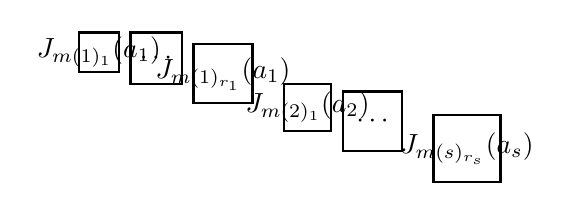
\begin{tikzpicture}[scale=0.5]
        \draw[thick] (0,0) rectangle (1,1);
        \node at (0.5,0.5) {\(J_{m(1)_1}(a_1)\)};

        \draw[thick] (1.3,-0.3) rectangle (2.6,1.0);
        \node at (1.95,0.35) {\(\cdots\)};

        \draw[thick] (2.9,-0.8) rectangle (4.4,0.7);
        \node at (3.65,-0.05) {\(J_{m(1)_{r_1}}(a_1)\)};

        \draw[thick] (5.2,-1.5) rectangle (6.4,-0.3);
        \node at (5.8,-0.9) {\(J_{m(2)_1}(a_2)\)};

        \draw[thick] (6.7,-2.0) rectangle (8.2,-0.5);
        \node at (7.45,-1.25) {\(\cdots\)};

        \draw[thick] (9.0,-2.8) rectangle (10.7,-1.1);
        \node at (9.85,-1.95) {\(J_{m(s)_{r_s}}(a_s)\)};
    \end{tikzpicture}
\]

\begin{snippetremark}{Similitudine}
    Date due matrici
    \[
        A,B\in \operatorname{Mat}_n(K),
    \]
    si ha
    \[
        A\sim B
    \]
    se e solo se hanno la stessa forma canonica razionale.

    Se \(K\) è algebricamente chiuso, questo equivale anche a dire che hanno la stessa forma canonica di Jordan, cioè gli stessi blocchi di Jordan a meno dell'ordine.
\end{snippetremark}

\begin{snippetexample}{Un esempio di forma di Jordan}
    Supponiamo che
    \[
        V\simeq
        \frac{K[X]}{(X-a)}
        \oplus
        \frac{K[X]}{(X-a)}
        \oplus
        \frac{K[X]}{((X-a)^3)}
        \oplus
        \frac{K[X]}{((X-b)^2)}
        \oplus
        \frac{K[X]}{((X-b)^2)},
    \]
    con \(a\neq b\).

    Allora \(\varphi\) ha forma di Jordan
    \[
        J_1(a)\oplus J_1(a)\oplus J_3(a)\oplus J_2(b)\oplus J_2(b).
    \]
    In particolare
    \[
        \chi_\varphi=(X-a)^5(X-b)^4.
    \]
    La matrice non è diagonalizzabile, perché compaiono blocchi di dimensione maggiore di \(1\).
\end{snippetexample}

\[
    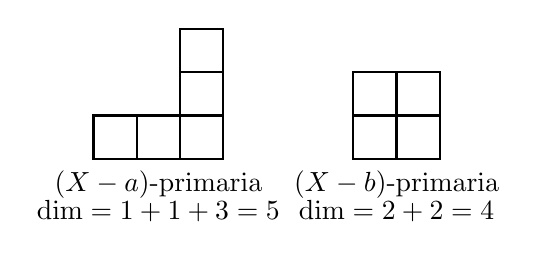
\begin{tikzpicture}[scale=0.55]
        \foreach \x/\h in {0/1,1/1,2/3} {
            \foreach \y in {1,...,\h} {
                \draw[thick] (\x,\y-1) rectangle (\x+1,\y);
            }
        }
        \node at (1.5,-0.6) {\((X-a)\)-primaria};
        \node at (1.5,-1.2) {\(\dim=1+1+3=5\)};

        \begin{scope}[xshift=6cm]
            \foreach \x/\h in {0/2,1/2} {
                \foreach \y in {1,...,\h} {
                    \draw[thick] (\x,\y-1) rectangle (\x+1,\y);
                }
            }
            \node at (1,-0.6) {\((X-b)\)-primaria};
            \node at (1,-1.2) {\(\dim=2+2=4\)};
        \end{scope}
    \end{tikzpicture}
\]

\subsection{Potenze dei blocchi di Jordan e rango}

Sia
\[
    J_m(a)=
    \begin{pmatrix}
        a & 1 & 0 & \cdots & 0\\
        0 & a & 1 & \cdots & 0\\
        0 & 0 & a & \ddots & \vdots\\
        \vdots & \vdots & \ddots & \ddots & 1\\
        0 & 0 & \cdots & 0 & a
    \end{pmatrix}.
\]
Scriviamo
\[
    J_m(a)=aI_m+N_m,
\]
dove
\[
    N_m=
    \begin{pmatrix}
        0 & 1 & 0 & \cdots & 0\\
        0 & 0 & 1 & \cdots & 0\\
        0 & 0 & 0 & \ddots & \vdots\\
        \vdots & \vdots & \ddots & \ddots & 1\\
        0 & 0 & \cdots & 0 & 0
    \end{pmatrix}.
\]
La matrice \(N_m\) è nilpotente:
\[
    N_m^m=0,
    \qquad
    N_m^{m-1}\neq 0.
\]

\begin{snippetproposition}{Rango delle potenze nilpotenti}
    Per ogni \(k\geq 0\),
    \[
        \operatorname{rk}(N_m^k)=
        \begin{cases}
            m-k & \text{se } 0\leq k\leq m,\\
            0 & \text{se } k\geq m.
        \end{cases}
    \]
    Equivalentemente,
    \[
        \dim_K\ker(N_m^k)=\min\{k,m\}.
    \]
\end{snippetproposition}

\begin{snippetproof}{}
    La matrice \(N_m\) manda
    \[
        e_1\mapsto 0,
        \qquad
        e_2\mapsto e_1,
        \qquad
        \ldots,
        \qquad
        e_m\mapsto e_{m-1}.
    \]
    Quindi \(N_m^k\) manda \(e_i\) in \(e_{i-k}\) se \(i>k\), e in \(0\) se \(i\leq k\).

    Pertanto l'immagine di \(N_m^k\) è generata da
    \[
        e_1,\ldots,e_{m-k}
    \]
    se \(k\leq m\), ed è nulla se \(k\geq m\).
    Da qui segue la formula per il rango.
\end{snippetproof}

\begin{snippetcorollary}{Lettura dei blocchi tramite i ranghi}
    Sia \(A\in\operatorname{Mat}_n(K)\) una matrice in forma di Jordan e sia \(a\in K\) un autovalore.
    Poniamo
    \[
        N_a=A-aI_n.
    \]
    La successione delle dimensioni
    \[
        \dim_K\ker(N_a),
        \qquad
        \dim_K\ker(N_a^2),
        \qquad
        \dim_K\ker(N_a^3),
        \qquad
        \ldots
    \]
    determina il numero e le dimensioni dei blocchi di Jordan relativi all'autovalore \(a\).

    Più precisamente,
    \[
        \dim_K\ker(N_a^k)-\dim_K\ker(N_a^{k-1})
    \]
    è il numero di blocchi di Jordan relativi ad \(a\) di dimensione almeno \(k\).
\end{snippetcorollary}

\begin{snippetproof}{}
    Su un blocco \(J_m(a)\), l'operatore \(N_a=A-aI_n\) diventa \(N_m\), e quindi
    \[
        \dim_K\ker(N_m^k)=\min\{k,m\}.
    \]
    Il contributo del blocco alla differenza
    \[
        \dim_K\ker(N_a^k)-\dim_K\ker(N_a^{k-1})
    \]
    è \(1\) se \(m\geq k\), ed è \(0\) se \(m<k\).

    Sommando sui blocchi, otteniamo esattamente il numero di blocchi di dimensione almeno \(k\).
\end{snippetproof}

\begin{snippetexample}{Ranghi nell'esempio precedente}
    Consideriamo
    \[
        A\simeq
        J_1(a)\oplus J_1(a)\oplus J_3(a)\oplus J_2(b)\oplus J_2(b),
        \qquad
        a\neq b.
    \]
    Poniamo
    \[
        \widetilde{A}=A-aI.
    \]
    Sulla componente relativa ad \(a\), la matrice \(\widetilde{A}\) ha ranghi
    \[
        2,\quad 1,\quad 0
    \]
    per le potenze prima, seconda e terza. Sulla componente relativa a \(b\), invece, \(\widetilde{A}\) è invertibile, quindi contribuisce sempre con rango \(4\). Dunque
    \[
        \operatorname{rk}(\widetilde{A})=2+4=6,
    \]
    \[
        \operatorname{rk}(\widetilde{A}^2)=1+4=5,
    \]
    \[
        \operatorname{rk}(\widetilde{A}^3)=0+4=4.
    \]
    Poiché la componente generalizzata relativa ad \(a\) ha dimensione \(5\), otteniamo:
    \[
        5-2=3
    \]
    blocchi relativi ad \(a\);
    poi
    \[
        5-1=4
    \]
    dà che un solo blocco ha altezza almeno \(2\), e
    \[
        5-0=5
    \]
    dà che un solo blocco ha altezza almeno \(3\).
    Quindi i blocchi relativi ad \(a\) hanno dimensioni
    \[
        1,\ 1,\ 3.
    \]

    Analogamente, per
    \[
        \widetilde{B}=A-bI,
    \]
    sulla componente relativa a \(b\) i ranghi sono
    \[
        2,\quad 0,\quad 0,
    \]
    mentre la componente relativa ad \(a\) contribuisce sempre con rango \(5\). Quindi
    \[
        \operatorname{rk}(\widetilde{B})=5+2=7,
    \]
    \[
        \operatorname{rk}(\widetilde{B}^2)=5+0=5,
    \]
    \[
        \operatorname{rk}(\widetilde{B}^3)=5.
    \]
    Da questo si legge che ci sono due blocchi relativi a \(b\), entrambi di dimensione \(2\).
\end{snippetexample}

\subsection{Esercizio: determinare una forma di Jordan}

\begin{snippetexercise}{}
    Determinare la forma canonica di Jordan della matrice
    \[
        A=
        \begin{pmatrix}
            2 & 0 & 0 & 0 & 0 & 0 & 0 & 0\\
            0 & 2 & 0 & 0 & 0 & 0 & 0 & 0\\
            0 & 3 & 1 & 0 & 1 & 0 & 0 & 0\\
            4 & 0 & 0 & 2 & 0 & 1 & 0 & 1\\
            0 & 0 & 0 & 0 & 1 & 2 & 0 & 0\\
            0 & 0 & 0 & 0 & 0 & 1 & 0 & 1\\
            0 & 0 & 0 & 0 & 0 & 0 & 2 & 0\\
            0 & 0 & 0 & 0 & 0 & 0 & 1 & 2
        \end{pmatrix}.
    \]
    Gli autovalori sono \(1\) e \(2\).
\end{snippetexercise}

\begin{snippetsolution}{}
    Il polinomio caratteristico è
    \[
        \chi_A(T)=(T-1)^3(T-2)^5.
    \]
    Quindi la componente generalizzata relativa all'autovalore \(1\) ha dimensione \(3\), mentre quella relativa all'autovalore \(2\) ha dimensione \(5\).

    Calcoliamo prima i ranghi delle potenze di
    \[
        A-I.
    \]
    Si ottiene
    \[
        \operatorname{rk}(A-I)=7,
    \]
    \[
        \operatorname{rk}\big((A-I)^2\big)=6,
    \]
    \[
        \operatorname{rk}\big((A-I)^3\big)=5.
    \]
    Dunque
    \[
        \dim\ker(A-I)=1,
    \]
    \[
        \dim\ker\big((A-I)^2\big)=2,
    \]
    \[
        \dim\ker\big((A-I)^3\big)=3.
    \]
    Le differenze successive sono
    \[
        1,\quad 1,\quad 1.
    \]
    Quindi, per l'autovalore \(1\), c'è un solo blocco di dimensione almeno \(1\), un solo blocco di dimensione almeno \(2\), e un solo blocco di dimensione almeno \(3\). Pertanto la componente relativa a \(1\) è un unico blocco:
    \[
        J_3(1).
    \]

    Passiamo all'autovalore \(2\). Calcoliamo i ranghi delle potenze di
    \[
        A-2I.
    \]
    Si ottiene
    \[
        \operatorname{rk}(A-2I)=5,
    \]
    \[
        \operatorname{rk}\big((A-2I)^2\big)=4,
    \]
    \[
        \operatorname{rk}\big((A-2I)^3\big)=3.
    \]
    Dunque
    \[
        \dim\ker(A-2I)=3,
    \]
    \[
        \dim\ker\big((A-2I)^2\big)=4,
    \]
    \[
        \dim\ker\big((A-2I)^3\big)=5.
    \]
    Le differenze successive sono
    \[
        3,\quad 1,\quad 1.
    \]
    Quindi, per l'autovalore \(2\), ci sono tre blocchi in totale, uno solo di dimensione almeno \(2\), e uno solo di dimensione almeno \(3\). Pertanto le dimensioni dei blocchi sono
    \[
        3,\quad 1,\quad 1.
    \]

    Concludiamo che la forma canonica di Jordan di \(A\) è
    \[
        J_3(1)\oplus J_3(2)\oplus J_1(2)\oplus J_1(2).
    \]
\end{snippetsolution}

\pagebreak
\part{Lezione 23}

\section{Polinomio minimo e forme canoniche}

\subsection{Il polinomio minimo}

\begin{snippetdefinition}{Polinomio minimo di una matrice}
    Sia
    \[
        A\in \operatorname{Mat}_n(K).
    \]
    Consideriamo l'insieme
    \[
        \mathcal{I}_A
        =
        \{f\in K[X]\mid f(A)=0\}.
    \]
    Il polinomio minimo di \(A\), denotato con
    \[
        \mu_A,
    \]
    è il generatore monico dell'ideale \(\mathcal{I}_A\).

    Equivalentemente, se \(A\) rappresenta un endomorfismo
    \[
        \varphi\colon V\to V
    \]
    rispetto a una base, allora \(\mu_A=\mu_\varphi\) è il polinomio monico di grado minimo tale che
    \[
        \mu_\varphi(\varphi)=0,
    \]
    cioè
    \[
        \mu_\varphi(\varphi)(v)=0
        \qquad
        \forall v\in V.
    \]
\end{snippetdefinition}

\begin{snippetproposition}{L'insieme dei polinomi annullanti è un ideale}
    L'insieme
    \[
        \mathcal{I}_A=\{f\in K[X]\mid f(A)=0\}
    \]
    è un ideale di \(K[X]\).
\end{snippetproposition}

\begin{snippetproof}{}
    Anzitutto \(0\in \mathcal{I}_A\), perché il polinomio nullo annulla \(A\).

    Se \(f,g\in \mathcal{I}_A\), allora
    \[
        (f+g)(A)=f(A)+g(A)=0+0=0,
    \]
    quindi \(f+g\in \mathcal{I}_A\).

    Inoltre, se \(g\in\mathcal{I}_A\) e \(h\in K[X]\), allora
    \[
        (hg)(A)=h(A)g(A)=h(A)0=0.
    \]
    Quindi \(hg\in \mathcal{I}_A\).

    Dunque \(\mathcal{I}_A\triangleleft K[X]\). Poiché \(K[X]\) è un dominio a ideali principali, esiste un unico polinomio monico \(\mu_A\) tale che
    \[
        \mathcal{I}_A=(\mu_A).
    \]
\end{snippetproof}

\begin{snippetremark}{}
    Il polinomio minimo è invariante per similitudine. Infatti, se
    \[
        B=P^{-1}AP,
        \qquad
        P\in \operatorname{GL}_n(K),
    \]
    allora, per ogni \(f\in K[X]\),
    \[
        f(B)=P^{-1}f(A)P.
    \]
    Quindi
    \[
        f(A)=0
        \iff
        f(B)=0.
    \]
    Pertanto
    \[
        \mu_A=\mu_B.
    \]
\end{snippetremark}

\begin{snippettheorem}{Polinomio minimo e blocchi di Jordan}
    Supponiamo che \(K\) sia algebricamente chiuso e che la forma di Jordan di \(A\) abbia, per gli autovalori distinti
    \[
        a_1,\ldots,a_s\in K,
    \]
    blocchi di dimensioni
    \[
        m(i)_1,\ldots,m(i)_{r_i}
    \]
    relativi all'autovalore \(a_i\).

    Poniamo
    \[
        n_i=\max\{m(i)_1,\ldots,m(i)_{r_i}\}.
    \]
    Allora
    \[
        \mu_A
        =
        \prod_{i=1}^s (X-a_i)^{n_i}.
    \]
\end{snippettheorem}

\begin{snippetproof}{}
    Possiamo supporre che \(A\) sia già in forma di Jordan, perché il polinomio minimo è invariante per similitudine.

    Consideriamo un blocco
    \[
        J_m(a)=aI_m+N_m,
    \]
    dove \(N_m\) è il blocco nilpotente con \(1\) sopra la diagonale principale.
    Allora
    \[
        (J_m(a)-aI_m)^m=N_m^m=0,
    \]
    mentre
    \[
        (J_m(a)-aI_m)^{m-1}=N_m^{m-1}\neq 0.
    \]
    Dunque il più piccolo esponente che annulla un blocco \(J_m(a)\) è proprio \(m\).

    Se prendiamo tutti i blocchi relativi allo stesso autovalore \(a_i\), il più piccolo esponente che li annulla simultaneamente è la dimensione massima tra questi blocchi, cioè
    \[
        n_i=\max\{m(i)_1,\ldots,m(i)_{r_i}\}.
    \]

    Pertanto il polinomio
    \[
        \prod_{i=1}^s (X-a_i)^{n_i}
    \]
    annulla tutti i blocchi di Jordan di \(A\), quindi annulla \(A\).

    Viceversa, se un polinomio
    \[
        g\in K[X]
    \]
    annulla \(A\), allora, per ogni autovalore \(a_i\), deve annullare tutti i blocchi relativi ad \(a_i\). In particolare deve essere divisibile da
    \[
        (X-a_i)^{n_i}.
    \]
    Poiché i fattori \((X-a_i)\) sono coprimi a due a due, segue che
    \[
        \prod_{i=1}^s (X-a_i)^{n_i}\mid g.
    \]
    Quindi questo prodotto è il generatore monico dell'ideale dei polinomi annullanti.
\end{snippetproof}

\begin{snippetcorollary}{Cayley-Hamilton}
    Ogni matrice quadrata annulla il proprio polinomio caratteristico:
    \[
        \chi_A(A)=0.
    \]
\end{snippetcorollary}

\begin{snippetproof}{}
    In forma di Jordan, il polinomio caratteristico è
    \[
        \chi_A(X)
        =
        \prod_{i=1}^s (X-a_i)^{N_i},
    \]
    dove \(N_i\) è la somma delle dimensioni di tutti i blocchi relativi all'autovalore \(a_i\).

    Poiché
    \[
        n_i\leq N_i
        \qquad
        \forall i,
    \]
    il polinomio minimo
    \[
        \mu_A=\prod_{i=1}^s (X-a_i)^{n_i}
    \]
    divide \(\chi_A\). Siccome \(\mu_A(A)=0\), anche
    \[
        \chi_A(A)=0.
    \]
\end{snippetproof}

\begin{snippetexample}{Lettura del polinomio minimo dai blocchi}
    Supponiamo che
    \[
        A\sim J_2(2)\oplus J_1(2)\oplus J_2(3).
    \]
    Allora gli autovalori sono \(2\) e \(3\). Per l'autovalore \(2\), il blocco più grande ha dimensione \(2\); per l'autovalore \(3\), il blocco più grande ha dimensione \(2\). Quindi
    \[
        \mu_A=(X-2)^2(X-3)^2.
    \]
    Invece il polinomio caratteristico è
    \[
        \chi_A=(X-2)^3(X-3)^2.
    \]
\end{snippetexample}

\begin{snippetexample}{Un esempio con polinomio caratteristico e minimo diversi}
    Supponiamo di aver determinato che una matrice \(A\) è simile a
    \[
        J_3(0)\oplus J_2(3)\oplus J_1(3).
    \]
    Allora
    \[
        \chi_A=X^3(X-3)^3,
    \]
    mentre il polinomio minimo è
    \[
        \mu_A=X^3(X-3)^2.
    \]
    Infatti l'esponente di \(X\) è la dimensione massima dei blocchi relativi all'autovalore \(0\), cioè \(3\), mentre l'esponente di \(X-3\) è la dimensione massima dei blocchi relativi all'autovalore \(3\), cioè \(2\).
\end{snippetexample}

\subsection{Esercizio: matrici simili}

\begin{snippetexercise}{}
    Stabilire quali tra le matrici
    \[
        A=
        \begin{pmatrix}
            2 & 0 & 0 & 0\\
            0 & 2 & 0 & 0\\
            2 & 0 & 2 & 1\\
            0 & 0 & 0 & 2
        \end{pmatrix},
    \]
    \[
        B=
        \begin{pmatrix}
            1 & 1 & 0 & 0\\
            -1 & 3 & 0 & 0\\
            -1 & 1 & 1 & 1\\
            -1 & 1 & -1 & 3
        \end{pmatrix},
    \]
    e
    \[
        C=
        \begin{pmatrix}
            2 & 1 & 1 & -1\\
            0 & 1 & 1 & -1\\
            0 & -1 & 3 & -1\\
            0 & 0 & 0 & 2
        \end{pmatrix}
    \]
    sono simili.
\end{snippetexercise}

\begin{snippetsolution}{}
    Tutte e tre hanno polinomio caratteristico
    \[
        \chi_A=\chi_B=\chi_C=(X-2)^4.
    \]
    Quindi l'unico autovalore è \(2\). Per distinguere le forme di Jordan calcoliamo i ranghi di
    \[
        A-2I_4,
        \qquad
        B-2I_4,
        \qquad
        C-2I_4.
    \]

    Per \(A\), si ha
    \[
        \operatorname{rk}(A-2I_4)=1.
    \]
    Quindi
    \[
        \dim\ker(A-2I_4)=4-1=3.
    \]
    Il numero di blocchi di Jordan relativi all'autovalore \(2\) è \(3\). Siccome la dimensione totale è \(4\), i blocchi sono
    \[
        2,\ 1,\ 1.
    \]
    Dunque
    \[
        J(A)=J_2(2)\oplus J_1(2)\oplus J_1(2).
    \]

    Per \(B\), si ha
    \[
        \operatorname{rk}(B-2I_4)=2,
    \]
    quindi
    \[
        \dim\ker(B-2I_4)=2.
    \]
    Ci sono dunque due blocchi. Inoltre
    \[
        (B-2I_4)^2=0,
    \]
    quindi nessun blocco ha dimensione maggiore di \(2\). Ne segue che
    \[
        J(B)=J_2(2)\oplus J_2(2).
    \]

    Per \(C\), si ha
    \[
        \operatorname{rk}(C-2I_4)=1,
    \]
    quindi
    \[
        \dim\ker(C-2I_4)=3.
    \]
    Anche qui ci sono tre blocchi, e quindi
    \[
        J(C)=J_2(2)\oplus J_1(2)\oplus J_1(2).
    \]

    Concludiamo che
    \[
        A\sim C,
        \qquad
        A\nsim B,
        \qquad
        B\nsim C.
    \]
    Inoltre
    \[
        \mu_A=\mu_C=(X-2)^2,
        \qquad
        \mu_B=(X-2)^2.
    \]
    In questo esempio il polinomio minimo non distingue \(A\) e \(B\): è necessario conoscere l'intera decomposizione in blocchi.
\end{snippetsolution}

\[
    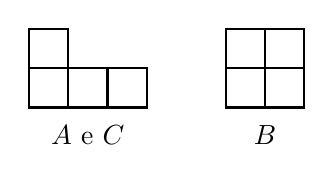
\begin{tikzpicture}[scale=0.5]
        \foreach \x/\h in {0/2,1/1,2/1} {
            \foreach \y in {1,...,\h} {
                \draw[thick] (\x,\y-1) rectangle (\x+1,\y);
            }
        }
        \node at (1.5,-0.7) {\(A\) e \(C\)};

        \begin{scope}[xshift=5cm]
            \foreach \x/\h in {0/2,1/2} {
                \foreach \y in {1,...,\h} {
                    \draw[thick] (\x,\y-1) rectangle (\x+1,\y);
                }
            }
            \node at (1,-0.7) {\(B\)};
        \end{scope}
    \end{tikzpicture}
\]

\subsection{Esempio su \(\rationalnumbers\) e \(\complexnumbers\)}

\begin{snippetexercise}{}
    Determinare la forma canonica della matrice
    \[
        A=
        \begin{pmatrix}
            1 & 0 & 0 & 0\\
            2 & 1 & 0 & 0\\
            0 & 0 & -\frac{1}{2} & -\frac{3}{2}\\
            0 & 0 & \frac{1}{2} & -\frac{1}{2}
        \end{pmatrix}
    \]
    prima su \(\rationalnumbers\), poi su \(\complexnumbers\).
\end{snippetexercise}

\begin{snippetsolution}{}
    Calcoliamo il polinomio caratteristico:
    \[
        \chi_A(X)
        =
        (X-1)^2(X^2+X+1).
    \]
    Il fattore
    \[
        f=X^2+X+1
    \]
    è irriducibile in \(\rationalnumbers[X]\), perché non ha radici razionali.

    Su \(\rationalnumbers\), la decomposizione primaria del modulo associato è
    \[
        \frac{\rationalnumbers[X]}{(X-1)^2}
        \oplus
        \frac{\rationalnumbers[X]}{(X^2+X+1)}.
    \]
    Poiché i due fattori sono coprimi, nella forma con fattori invarianti otteniamo un solo fattore:
    \[
        \frac{\rationalnumbers[X]}{\big((X-1)^2(X^2+X+1)\big)}.
    \]
    Quindi la forma canonica razionale è la matrice compagna
    \[
        C\big((X-1)^2(X^2+X+1)\big).
    \]

    Su \(\complexnumbers\), invece,
    \[
        X^2+X+1=(X-\omega)(X-\omega^2),
    \]
    dove
    \[
        \omega=-\frac{1}{2}+\frac{\sqrt{3}}{2}i,
        \qquad
        \omega^2=-\frac{1}{2}-\frac{\sqrt{3}}{2}i.
    \]
    Dunque
    \[
        \chi_A(X)=(X-1)^2(X-\omega)(X-\omega^2).
    \]

    Calcoliamo inoltre
    \[
        \operatorname{rk}(A-I_4)=3,
    \]
    quindi
    \[
        \dim\ker(A-I_4)=1.
    \]
    Poiché la molteplicità algebrica dell'autovalore \(1\) è \(2\), il blocco relativo a \(1\) è unico e ha dimensione \(2\).

    Pertanto, su \(\complexnumbers\), la forma di Jordan è
    \[
        J(A)=J_2(1)\oplus J_1(\omega)\oplus J_1(\omega^2).
    \]
\end{snippetsolution}

\subsection{Polinomi di matrici e forma di Jordan}

\begin{snippetproposition}{Forma di Jordan di un polinomio in una matrice}
    Sia
    \[
        B=f(A),
        \qquad
        f\in K[X].
    \]
    Se
    \[
        J(A)=P^{-1}AP
    \]
    è una forma di Jordan di \(A\), allora
    \[
        f(J(A))=P^{-1}f(A)P=P^{-1}BP.
    \]
    Quindi \(B\) è simile a \(f(J(A))\).

    Attenzione: la matrice \(f(J(A))\) non è necessariamente già in forma di Jordan; bisogna eventualmente ridurla ancora.
\end{snippetproposition}

\begin{snippetproof}{}
    Se
    \[
        J(A)=P^{-1}AP,
    \]
    allora, per ogni \(m\geq 0\),
    \[
        J(A)^m=P^{-1}A^mP.
    \]
    Quindi, per
    \[
        f=\sum_m c_mX^m,
    \]
    si ha
    \[
        f(J(A))
        =
        \sum_m c_mJ(A)^m
        =
        \sum_m c_mP^{-1}A^mP
        =
        P^{-1}f(A)P.
    \]
\end{snippetproof}

\begin{snippetexample}{Il caso \(B=A+A^2\)}
    Supponiamo che
    \[
        J(A)=J_3(0)\oplus J_2(3)\oplus J_1(3).
    \]
    Poniamo
    \[
        B=A+A^2.
    \]
    Allora
    \[
        B=f(A),
        \qquad
        f(X)=X+X^2.
    \]
    Gli autovalori vengono trasformati da \(f\):
    \[
        f(0)=0,
        \qquad
        f(3)=12.
    \]
    Quindi
    \[
        \chi_B=X^3(X-12)^3.
    \]

    Poiché
    \[
        f'(X)=1+2X,
    \]
    abbiamo
    \[
        f'(0)=1\neq 0,
        \qquad
        f'(3)=7\neq 0.
    \]
    In questo caso le dimensioni dei blocchi vengono preservate. Pertanto
    \[
        J(B)=J_3(0)\oplus J_2(12)\oplus J_1(12).
    \]

    In particolare,
    \[
        \mu_B=X^3(X-12)^2.
    \]

    Nella forma con fattori invarianti, la parte relativa a \(0\) ha un blocco di dimensione \(3\), mentre la parte relativa a \(12\) ha blocchi di dimensioni \(1\) e \(2\). Allineando le colonne, otteniamo
    \[
        V_B\simeq
        \frac{K[X]}{(X-12)}
        \oplus
        \frac{K[X]}{\big(X^3(X-12)^2\big)}.
    \]
    Quindi i fattori invarianti sono
    \[
        X-12,
        \qquad
        X^3(X-12)^2.
    \]
\end{snippetexample}

\[
    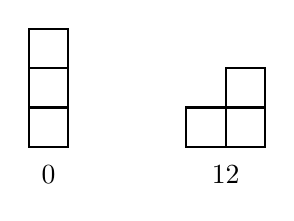
\begin{tikzpicture}[scale=0.5]
        \foreach \x/\h in {0/3} {
            \foreach \y in {1,...,\h} {
                \draw[thick] (\x,\y-1) rectangle (\x+1,\y);
            }
        }
        \node at (0.5,-0.7) {\(0\)};

        \begin{scope}[xshift=4cm]
            \foreach \x/\h in {0/1,1/2} {
                \foreach \y in {1,...,\h} {
                    \draw[thick] (\x,\y-1) rectangle (\x+1,\y);
                }
            }
            \node at (1,-0.7) {\(12\)};
        \end{scope}
    \end{tikzpicture}
\]

\subsection{Esercizio con parametri}

\begin{snippetexercise}{}
    Siano
    \[
        \alpha,\beta,\gamma\in\complexnumbers
    \]
    e consideriamo
    \[
        A=
        \begin{pmatrix}
            1 & 0 & 0 & \gamma\\
            0 & 1 & 0 & 0\\
            0 & \alpha & 4 & -3\\
            0 & \beta & 3 & -2
        \end{pmatrix}
        \in\operatorname{Mat}_4(\complexnumbers).
    \]
    Determinare la forma canonica di Jordan di \(A\) in funzione di \(\alpha,\beta,\gamma\).
\end{snippetexercise}

\begin{snippetsolution}{}
    Calcoliamo il polinomio caratteristico:
    \[
        \chi_A(X)
        =
        \det(XI_4-A).
    \]
    Sviluppando lungo la prima colonna, si ottiene
    \begin{align*}
        \chi_A(X)
        &=
        (X-1)^2
        \det
        \begin{pmatrix}
            X-4 & 3\\
            -3 & X+2
        \end{pmatrix} \\
        &=
        (X-1)^2\big((X-4)(X+2)+9\big) \\
        &=
        (X-1)^2(X^2-2X+1) \\
        &=
        (X-1)^4.
    \end{align*}
    Quindi l'unico autovalore è \(1\).

    Poniamo
    \[
        N=A-I_4.
    \]
    Allora
    \[
        N=
        \begin{pmatrix}
            0 & 0 & 0 & \gamma\\
            0 & 0 & 0 & 0\\
            0 & \alpha & 3 & -3\\
            0 & \beta & 3 & -3
        \end{pmatrix}.
    \]
    La forma di Jordan è determinata dai ranghi di \(N,N^2,\ldots\).

    \textbf{Caso 1: \(\gamma=0\).}

    In questo caso
    \[
        N=
        \begin{pmatrix}
            0 & 0 & 0 & 0\\
            0 & 0 & 0 & 0\\
            0 & \alpha & 3 & -3\\
            0 & \beta & 3 & -3
        \end{pmatrix}.
    \]

    Se
    \[
        \alpha=\beta,
    \]
    allora le due righe non nulle sono uguali, quindi
    \[
        \operatorname{rk}(N)=1.
    \]
    Dunque
    \[
        \dim\ker(N)=4-1=3,
    \]
    cioè ci sono tre blocchi di Jordan. Poiché la dimensione totale è \(4\), le dimensioni dei blocchi sono
    \[
        2,\ 1,\ 1.
    \]
    Quindi
    \[
        J(A)=J_2(1)\oplus J_1(1)\oplus J_1(1).
    \]

    Se invece
    \[
        \alpha\neq \beta,
    \]
    allora
    \[
        \det
        \begin{pmatrix}
            \alpha & 3\\
            \beta & 3
        \end{pmatrix}
        =
        3\alpha-3\beta
        =
        3(\alpha-\beta)\neq 0.
    \]
    Quindi
    \[
        \operatorname{rk}(N)=2,
    \]
    e dunque ci sono
    \[
        4-2=2
    \]
    blocchi di Jordan.

    Inoltre
    \[
        \operatorname{rk}(N^2)=1.
    \]
    Ne segue che esiste un blocco di dimensione \(3\). Quindi le dimensioni dei blocchi sono
    \[
        3,\ 1,
    \]
    e
    \[
        J(A)=J_3(1)\oplus J_1(1).
    \]

    \textbf{Caso 2: \(\gamma\neq 0\).}

    Se
    \[
        \alpha=\beta,
    \]
    allora si verifica che
    \[
        \operatorname{rk}(N)=2,
    \]
    quindi ci sono due blocchi. Inoltre
    \[
        \operatorname{rk}(N^2)=1,
    \]
    quindi uno dei due blocchi ha dimensione \(3\). Pertanto
    \[
        J(A)=J_3(1)\oplus J_1(1).
    \]

    Se invece
    \[
        \alpha\neq \beta,
    \]
    allora le colonne indipendenti sono tre, perché la colonna contenente \(\gamma\) è indipendente dalle colonne che hanno prima coordinata nulla, e le colonne
    \[
        \begin{pmatrix}
            0\\
            0\\
            \alpha\\
            \beta
        \end{pmatrix},
        \qquad
        \begin{pmatrix}
            0\\
            0\\
            3\\
            3
        \end{pmatrix}
    \]
    sono indipendenti.
    Quindi
    \[
        \operatorname{rk}(N)=3.
    \]
    Pertanto
    \[
        \dim\ker(N)=1,
    \]
    cioè c'è un solo blocco di Jordan. Siccome la dimensione totale è \(4\), abbiamo
    \[
        J(A)=J_4(1).
    \]

    Riassumendo:
    \[
        J(A)=
        \begin{cases}
            J_2(1)\oplus J_1(1)\oplus J_1(1)
            & \text{se } \gamma=0,\ \alpha=\beta,\\[4pt]
            J_3(1)\oplus J_1(1)
            & \text{se } \gamma=0,\ \alpha\neq \beta,\\[4pt]
            J_3(1)\oplus J_1(1)
            & \text{se } \gamma\neq 0,\ \alpha=\beta,\\[4pt]
            J_4(1)
            & \text{se } \gamma\neq 0,\ \alpha\neq \beta.
        \end{cases}
    \]
\end{snippetsolution}

\pagebreak
\part{Lezione 24}

\section{Elementi di dato ordine nei gruppi abeliani finiti}

\subsection{Il caso ciclico}

\begin{snippetdefinition}{Funzione di Eulero}
    Per \(n\geq 1\), la funzione di Eulero è
    \[
        \varphi(n)
        =
        \#\{1\leq k\leq n\mid \gcd(k,n)=1\}.
    \]
\end{snippetdefinition}

Ricordiamo alcune proprietà:
\[
    \varphi(p)=p-1
\]
se \(p\) è primo,
\[
    \varphi(p^r)=p^r-p^{r-1}=p^{r-1}(p-1),
\]
e, se \(\gcd(n_1,n_2)=1\), allora
\[
    \varphi(n_1n_2)=\varphi(n_1)\varphi(n_2).
\]

\begin{snippetproposition}{Ordine degli elementi in un gruppo ciclico}
    Sia
    \[
        G=\langle g\rangle
    \]
    un gruppo ciclico di ordine
    \[
        |G|=\operatorname{ord}(g)=n.
    \]
    Allora, per ogni \(0\leq k\leq n-1\),
    \[
        \operatorname{ord}(g^k)
        =
        \frac{n}{\gcd(k,n)}.
    \]
    In particolare,
    \[
        g^k \text{ genera } G
        \iff
        \gcd(k,n)=1.
    \]
\end{snippetproposition}

\begin{snippetproof}{}
    L'ordine di \(g^k\) è il minimo intero positivo \(d\) tale che
    \[
        (g^k)^d=1_G.
    \]
    Questa condizione equivale a
    \[
        g^{kd}=1_G,
    \]
    cioè
    \[
        n\mid kd.
    \]
    Scriviamo
    \[
        m=\gcd(k,n),
        \qquad
        k=mk',
        \qquad
        n=mn',
    \]
    con
    \[
        \gcd(k',n')=1.
    \]
    Allora
    \[
        n\mid kd
        \iff
        mn'\mid mk'd
        \iff
        n'\mid k'd.
    \]
    Poiché \(\gcd(k',n')=1\), questo equivale a
    \[
        n'\mid d.
    \]
    Il minimo tale \(d\) è quindi
    \[
        d=n'=\frac{n}{m}=\frac{n}{\gcd(k,n)}.
    \]
\end{snippetproof}

\begin{snippetcorollary}{Numero di generatori di un gruppo ciclico}
    Se \(G\) è ciclico di ordine \(n\), allora il numero di generatori di \(G\) è
    \[
        \varphi(n).
    \]
\end{snippetcorollary}

\begin{snippetproof}{}
    Gli elementi di \(G\) sono
    \[
        1,g,g^2,\ldots,g^{n-1}.
    \]
    Per la proposizione precedente, \(g^k\) è un generatore se e solo se
    \[
        \gcd(k,n)=1.
    \]
    Quindi il numero di generatori è precisamente
    \[
        \#\{1\leq k\leq n\mid \gcd(k,n)=1\}
        =
        \varphi(n).
    \]
\end{snippetproof}

\begin{snippetproposition}{Elementi di ordine fissato in un gruppo ciclico}
    Sia \(G=\langle g\rangle\) un gruppo ciclico di ordine \(n\). Se
    \[
        d\mid n,
    \]
    allora \(G\) contiene esattamente
    \[
        \varphi(d)
    \]
    elementi di ordine \(d\).
\end{snippetproposition}

\begin{snippetproof}{}
    L'elemento
    \[
        g^{n/d}
    \]
    ha ordine \(d\), perché
    \[
        \left(g^{n/d}\right)^d=g^n=1_G,
    \]
    e nessuna potenza positiva minore di \(d\) dà l'identità.

    Quindi
    \[
        H=\langle g^{n/d}\rangle
    \]
    è l'unico sottogruppo ciclico di \(G\) di ordine \(d\). Gli elementi di ordine esattamente \(d\) sono precisamente i generatori di \(H\).

    Siccome \(H\) è ciclico di ordine \(d\), ha
    \[
        \varphi(d)
    \]
    generatori. Dunque \(G\) ha esattamente \(\varphi(d)\) elementi di ordine \(d\).
\end{snippetproof}

\begin{snippetremark}{}
    Si ottiene anche l'identità
    \[
        \sum_{d\mid n}\varphi(d)=n.
    \]
    Infatti ogni elemento di un gruppo ciclico di ordine \(n\) ha ordine un divisore di \(n\), e per ogni divisore \(d\mid n\) ci sono \(\varphi(d)\) elementi di ordine \(d\).
\end{snippetremark}

\subsection{Prodotti diretti di gruppi ciclici}

\begin{snippetproposition}{Ordine di un elemento in un prodotto diretto}
    Siano \(G_1,\ldots,G_r\) gruppi finiti, e sia
    \[
        x=(x_1,\ldots,x_r)\in G_1\times\cdots\times G_r.
    \]
    Allora
    \[
        \operatorname{ord}(x)
        =
        \operatorname{mcm}\big(
            \operatorname{ord}(x_1),\ldots,\operatorname{ord}(x_r)
        \big).
    \]
\end{snippetproposition}

\begin{snippetproof}{}
    Per ogni \(k\geq 1\),
    \[
        x^k=(x_1^k,\ldots,x_r^k).
    \]
    Quindi
    \[
        x^k=1
        \iff
        x_i^k=1
        \qquad
        \forall i.
    \]
    Questo equivale a dire che
    \[
        \operatorname{ord}(x_i)\mid k
        \qquad
        \forall i.
    \]
    Il minimo intero positivo con questa proprietà è il minimo comune multiplo degli ordini delle componenti.
\end{snippetproof}

\begin{snippetexample}{Prodotto di due ciclici}
    Siano
    \[
        G=C_n\times C_m,
    \]
    con
    \[
        C_n=\langle g\rangle,
        \qquad
        C_m=\langle h\rangle.
    \]
    Gli elementi di \(G\) sono della forma
    \[
        (g^{k_1},h^{k_2}),
    \]
    e
    \[
        \operatorname{ord}(g^{k_1},h^{k_2})
        =
        \operatorname{mcm}
        \left(
            \operatorname{ord}(g^{k_1}),
            \operatorname{ord}(h^{k_2})
        \right).
    \]
\end{snippetexample}

\subsection{Esempio: gruppi abeliani di ordine \(100\)}

\begin{snippetexample}{Classificazione dei gruppi abeliani di ordine \(100\)}
    Poiché
    \[
        100=2^2\cdot 5^2,
    \]
    per ogni primo \(p=2,5\) ci sono due possibilità per la componente \(p\)-primaria:
    \[
        C_p\times C_p,
        \qquad
        C_{p^2}.
    \]
    Quindi, a meno di isomorfismo, i gruppi abeliani di ordine \(100\) sono:
    \[
        C_{100},
        \qquad
        C_5\times C_{20},
        \qquad
        C_2\times C_{50},
        \qquad
        C_{10}\times C_{10}.
    \]
\end{snippetexample}

\[
    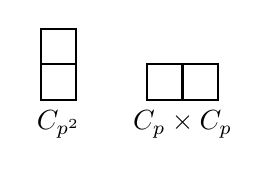
\begin{tikzpicture}[scale=0.45]
        \foreach \x/\h in {0/2} {
            \foreach \y in {1,...,\h} {
                \draw[thick] (\x,\y-1) rectangle (\x+1,\y);
            }
        }
        \node at (0.5,-0.7) {\(C_{p^2}\)};

        \begin{scope}[xshift=3cm]
            \foreach \x/\h in {0/1,1/1} {
                \foreach \y in {1,...,\h} {
                    \draw[thick] (\x,\y-1) rectangle (\x+1,\y);
                }
            }
            \node at (1,-0.7) {\(C_p\times C_p\)};
        \end{scope}
    \end{tikzpicture}
\]

\begin{snippetexample}{Elementi di dato ordine nei gruppi di ordine \(100\)}
    Per \(C_{100}\), essendo ciclico, il numero di elementi di ordine \(d\mid 100\) è \(\varphi(d)\):
    \[
        \begin{array}{c|ccccccccc}
            d & 1 & 2 & 4 & 5 & 10 & 20 & 25 & 50 & 100\\
            \hline
            \#\{x\mid \operatorname{ord}(x)=d\}
              & 1 & 1 & 2 & 4 & 4 & 8 & 20 & 20 & 40
        \end{array}
    \]

    Per
    \[
        C_5\times C_{20},
    \]
    gli ordini possibili sono
    \[
        1,2,4,5,10,20,
    \]
    e si ottiene:
    \[
        \begin{array}{c|cccccc}
            d & 1 & 2 & 4 & 5 & 10 & 20\\
            \hline
            \#\{x\mid \operatorname{ord}(x)=d\}
              & 1 & 1 & 2 & 24 & 24 & 48
        \end{array}
    \]

    Per
    \[
        C_2\times C_{50},
    \]
    gli ordini possibili sono
    \[
        1,2,5,10,25,50,
    \]
    e si ottiene:
    \[
        \begin{array}{c|cccccc}
            d & 1 & 2 & 5 & 10 & 25 & 50\\
            \hline
            \#\{x\mid \operatorname{ord}(x)=d\}
              & 1 & 3 & 4 & 12 & 20 & 60
        \end{array}
    \]

    Per
    \[
        C_{10}\times C_{10},
    \]
    gli ordini possibili sono
    \[
        1,2,5,10,
    \]
    e si ottiene:
    \[
        \begin{array}{c|cccc}
            d & 1 & 2 & 5 & 10\\
            \hline
            \#\{x\mid \operatorname{ord}(x)=d\}
              & 1 & 3 & 24 & 72
        \end{array}
    \]
\end{snippetexample}

\begin{snippetproof}{Idea del calcolo}
    Per esempio, in \(C_5\times C_{20}\), un elemento ha ordine
    \[
        \operatorname{mcm}(d_1,d_2),
    \]
    dove
    \[
        d_1\in\{1,5\},
        \qquad
        d_2\in\{1,2,4,5,10,20\}.
    \]
    Per contare gli elementi di ordine \(d\), si sommano i prodotti
    \[
        \varphi(d_1)\varphi(d_2)
    \]
    su tutte le coppie \((d_1,d_2)\) tali che
    \[
        \operatorname{mcm}(d_1,d_2)=d.
    \]
    Lo stesso metodo vale per gli altri prodotti diretti.
\end{snippetproof}

\section{Esercizi sui gruppi abeliani finiti}

\begin{snippetexercise}{Gruppi ciclici e prodotti diretti}
    Determinare quali tra i seguenti gruppi sono isomorfi:
    \[
        C_4\times C_9,
        \qquad
        C_6\times C_6,
        \qquad
        C_8\times C_3,
        \qquad
        C_9\times C_4,
        \qquad
        C_6\times C_4,
        \qquad
        C_{24}.
    \]
\end{snippetexercise}

\begin{snippetsolution}{}
    Usiamo il fatto che
    \[
        C_m\times C_n\simeq C_{mn}
        \iff
        \gcd(m,n)=1.
    \]

    Siccome
    \[
        \gcd(4,9)=1,
    \]
    abbiamo
    \[
        C_4\times C_9\simeq C_{36}.
    \]
    Analogamente
    \[
        C_9\times C_4\simeq C_{36}.
    \]
    Quindi
    \[
        C_4\times C_9\simeq C_9\times C_4.
    \]

    Inoltre
    \[
        \gcd(8,3)=1,
    \]
    dunque
    \[
        C_8\times C_3\simeq C_{24}.
    \]

    Invece
    \[
        C_6\times C_6
    \]
    non è ciclico, perché l'ordine massimo di un suo elemento è \(6\), mentre il gruppo ha ordine \(36\).

    Infine
    \[
        C_6\times C_4
        \simeq
        C_3\times C_2\times C_4
        \simeq
        C_2\times C_{12}.
    \]
    Questo gruppo ha ordine \(24\), ma non è ciclico, perché l'ordine massimo di un elemento è \(12\). Quindi
    \[
        C_6\times C_4\not\cong C_{24}.
    \]

    Le classi di isomorfismo sono quindi:
    \[
        \{C_4\times C_9,\ C_9\times C_4\},
    \]
    \[
        \{C_8\times C_3,\ C_{24}\},
    \]
    \[
        \{C_6\times C_6\},
    \]
    \[
        \{C_6\times C_4\}.
    \]
\end{snippetsolution}

\begin{snippetexercise}{Gruppi con ordini degli elementi che dividono \(28\)}
    Determinare tutti i gruppi abeliani finiti \(G\) tali che
    \[
        30\leq |G|\leq 60
    \]
    e, per ogni
    \[
        g\in G,
    \]
    si abbia
    \[
        \operatorname{ord}(g)\mid 28.
    \]
\end{snippetexercise}

\begin{snippetsolution}{}
    Poiché ogni ordine degli elementi divide \(28\), se un primo \(p\) divide \(|G|\), per il teorema di Cauchy esiste un elemento di ordine \(p\). Quindi
    \[
        p\mid 28.
    \]
    I soli primi possibili sono
    \[
        2
        \qquad
        \text{e}
        \qquad
        7.
    \]
    Dunque
    \[
        |G|=2^a7^b.
    \]
    Con la condizione
    \[
        30\leq |G|\leq 60,
    \]
    le possibilità sono:
    \[
        |G|=32,
        \qquad
        |G|=49,
        \qquad
        |G|=56.
    \]

    \textbf{Caso \(|G|=32=2^5\).}
    Poiché ogni elemento deve avere ordine che divide \(28\), la parte \(2\)-primaria può avere esponente al più \(4\). Quindi non possono comparire fattori ciclici \(C_8,C_{16},C_{32}\).
    Le possibilità sono:
    \[
        C_4\times C_4\times C_2,
        \qquad
        C_4\times C_2\times C_2\times C_2,
        \qquad
        C_2^5.
    \]

    \textbf{Caso \(|G|=49=7^2\).}
    Le possibilità astratte sono
    \[
        C_{49},
        \qquad
        C_7\times C_7.
    \]
    Ma \(C_{49}\) contiene elementi di ordine \(49\), e
    \[
        49\nmid 28.
    \]
    Quindi resta solo
    \[
        C_7\times C_7.
    \]

    \textbf{Caso \(|G|=56=2^3\cdot 7\).}
    La parte \(7\)-primaria è necessariamente \(C_7\). La parte \(2\)-primaria di ordine \(8\) può essere:
    \[
        C_8,
        \qquad
        C_4\times C_2,
        \qquad
        C_2\times C_2\times C_2.
    \]
    Il fattore \(C_8\) non è ammesso, perché contiene elementi di ordine \(8\), e
    \[
        8\nmid 28.
    \]
    Restano dunque:
    \[
        C_4\times C_2\times C_7
        \simeq
        C_2\times C_{28},
    \]
    e
    \[
        C_2\times C_2\times C_2\times C_7
        \simeq
        C_2\times C_2\times C_{14}.
    \]

    Quindi i gruppi cercati sono:
    \[
        C_4\times C_4\times C_2,
        \qquad
        C_4\times C_2\times C_2\times C_2,
        \qquad
        C_2^5,
    \]
    \[
        C_7\times C_7,
    \]
    \[
        C_2\times C_{28},
        \qquad
        C_2\times C_2\times C_{14}.
    \]
\end{snippetsolution}

\section{Esercizio: forma di Jordan al variare di un parametro}

\begin{snippetexercise}{}
    Sia
    \[
        A=
        \begin{pmatrix}
            1 & 0 & 1 & 0\\
            0 & 1 & 0 & 0\\
            0 & 0 & 5 & 3\\
            0 & t & -3 & -1
        \end{pmatrix}
        \in \operatorname{Mat}_4(\rationalnumbers),
        \qquad
        t\in\rationalnumbers.
    \]
    Determinare il polinomio minimo e la forma di Jordan di \(A\) al variare di \(t\).
\end{snippetexercise}

\begin{snippetsolution}{}
    Calcoliamo il polinomio caratteristico:
    \[
        \chi_A(X)
        =
        \det(XI_4-A)
        =
        (X-1)^2(X-2)^2.
    \]
    Gli autovalori sono quindi
    \[
        1
        \qquad
        \text{e}
        \qquad
        2,
    \]
    entrambi con molteplicità algebrica \(2\).

    Studiamo prima l'autovalore \(1\). Si ha
    \[
        A-I_4=
        \begin{pmatrix}
            0 & 0 & 1 & 0\\
            0 & 0 & 0 & 0\\
            0 & 0 & 4 & 3\\
            0 & t & -3 & -2
        \end{pmatrix}.
    \]
    Se
    \[
        t=0,
    \]
    allora
    \[
        \operatorname{rk}(A-I_4)=2,
    \]
    dunque
    \[
        \dim\ker(A-I_4)=2.
    \]
    Quindi, relativamente all'autovalore \(1\), ci sono due blocchi di Jordan. Poiché la molteplicità algebrica di \(1\) è \(2\), i due blocchi sono entrambi di dimensione \(1\).

    Se invece
    \[
        t\neq 0,
    \]
    allora una sottomatrice \(3\times 3\) ha determinante non nullo, e si ottiene
    \[
        \operatorname{rk}(A-I_4)=3.
    \]
    Quindi
    \[
        \dim\ker(A-I_4)=1,
    \]
    e per l'autovalore \(1\) compare un unico blocco di dimensione \(2\), cioè
    \[
        J_2(1).
    \]

    Studiamo ora l'autovalore \(2\). Si ha
    \[
        A-2I_4=
        \begin{pmatrix}
            -1 & 0 & 1 & 0\\
            0 & -1 & 0 & 0\\
            0 & 0 & 3 & 3\\
            0 & t & -3 & -3
        \end{pmatrix}.
    \]
    Per ogni \(t\in\rationalnumbers\) si ha
    \[
        \operatorname{rk}(A-2I_4)=3.
    \]
    Quindi
    \[
        \dim\ker(A-2I_4)=1.
    \]
    Siccome la molteplicità algebrica di \(2\) è \(2\), il blocco relativo all'autovalore \(2\) è sempre
    \[
        J_2(2).
    \]

    Concludiamo:
    \[
        J(A)=
        \begin{cases}
            J_1(1)\oplus J_1(1)\oplus J_2(2)
            & \text{se } t=0,\\[4pt]
            J_2(1)\oplus J_2(2)
            & \text{se } t\neq 0.
        \end{cases}
    \]

    Di conseguenza il polinomio minimo è:
    \[
        \mu_A=
        \begin{cases}
            (X-1)(X-2)^2
            & \text{se } t=0,\\[4pt]
            (X-1)^2(X-2)^2
            & \text{se } t\neq 0.
        \end{cases}
    \]
\end{snippetsolution}

\section{Esercizio: un quoziente di \(\rationalnumbers[X]\)}

\begin{snippetexercise}{}
    Sia
    \[
        f=X^3-3X^2-X-1\in\rationalnumbers[X].
    \]
    Mostrare che
    \[
        A=\rationalnumbers[X]/(f)
    \]
    è un campo e trovare l'inverso di
    \[
        (X^2+1)+(f)
    \]
    in \(A\).
\end{snippetexercise}

\begin{snippetsolution}{}
    Il polinomio \(f\) ha grado \(3\). Per mostrare che è irriducibile in \(\rationalnumbers[X]\), basta verificare che non abbia radici razionali.

    Per il criterio delle radici razionali, le uniche radici razionali possibili sono
    \[
        1
        \qquad
        \text{e}
        \qquad
        -1.
    \]
    Ma
    \[
        f(1)=1-3-1-1=-4\neq 0,
    \]
    e
    \[
        f(-1)=-1-3+1-1=-4\neq 0.
    \]
    Quindi \(f\) non ha radici razionali, e dunque è irriducibile.

    Pertanto l'ideale
    \[
        (f)\triangleleft \rationalnumbers[X]
    \]
    è massimale, e quindi
    \[
        A=\rationalnumbers[X]/(f)
    \]
    è un campo.

    Poniamo
    \[
        g=X^2+1.
    \]
    Vogliamo trovare \(h\in\rationalnumbers[X]\) tale che
    \[
        gh\equiv 1\pmod f.
    \]

    Usiamo l'algoritmo di Euclide. Dividendo \(f\) per \(g\), otteniamo
    \[
        f=(X-3)g-2(X-1).
    \]
    Quindi
    \[
        X-1=\frac{1}{2}\big((X-3)g-f\big).
    \]
    Inoltre
    \[
        g=(X-1)(X+1)+2.
    \]
    Da questa uguaglianza segue
    \[
        1=\frac{1}{2}g-\frac{1}{2}(X-1)(X+1).
    \]
    Sostituendo l'espressione di \(X-1\), otteniamo
    \begin{align*}
        1
        &=
        \frac{1}{2}g
        -
        \frac{1}{2}
        \left[
            \frac{1}{2}\big((X-3)g-f\big)
        \right](X+1) \\
        &=
        \left(
            \frac{1}{2}
            -
            \frac{1}{4}(X-3)(X+1)
        \right)g
        +
        \frac{1}{4}(X+1)f.
    \end{align*}
    Passando al quoziente modulo \((f)\), il termine multiplo di \(f\) scompare. Quindi
    \[
        \big((X^2+1)+(f)\big)^{-1}
        =
        \left(
            \frac{1}{2}
            -
            \frac{1}{4}(X-3)(X+1)
        \right)
        +(f).
    \]
    Equivalentemente,
    \[
        \big((X^2+1)+(f)\big)^{-1}
        =
        \left(
            -\frac{1}{4}X^2+\frac{1}{2}X+\frac{5}{4}
        \right)
        +(f).
    \]
\end{snippetsolution}

\pagebreak
\part{Lezione 25}

\section{Esercizi su forme canoniche e quozienti}

\begin{snippetexercise}{Forma canonica su \(\rationalnumbers\) e su \(\realnumbers\)}
    Sia
    \[
        A=
        \begin{pmatrix}
            1 & 0 & 0 & -2 & -1\\
            1 & 0 & 0 & 2 & 1\\
            0 & 1 & 2 & 1 & 0\\
            -1 & 2 & 0 & 0 & -1\\
            1 & -2 & 0 & 2 & 3
        \end{pmatrix}.
    \]
    Determinare i divisori elementari e la forma canonica di \(A\) su \(\rationalnumbers\) e su \(\realnumbers\).
\end{snippetexercise}

\begin{snippetsolution}{}
    Calcoliamo il polinomio caratteristico:
    \[
        \chi_A(X)=\det(XI_5-A).
    \]
    Sviluppando rispetto alla terza colonna, si ottiene
    \[
        \chi_A(X)=(X-2)^3(X^2-2)\in \rationalnumbers[X].
    \]
    In particolare, su \(\rationalnumbers\) il polinomio caratteristico ha fattori irriducibili
    \[
        X-2,
        \qquad
        X^2-2,
    \]
    mentre su \(\realnumbers\) si spezza come
    \[
        \chi_A(X)=(X-2)^3(X-\sqrt{2})(X+\sqrt{2}).
    \]

    Studiamo prima l'autovalore \(2\). Calcoliamo
    \[
        A-2I_5=
        \begin{pmatrix}
            -1 & 0 & 0 & -2 & -1\\
            1 & -2 & 0 & 2 & 1\\
            0 & 1 & 0 & 1 & 0\\
            -1 & 2 & 0 & -2 & -1\\
            1 & -2 & 0 & 2 & 1
        \end{pmatrix}.
    \]
    Si ha
    \[
        \operatorname{rk}(A-2I_5)=3,
    \]
    dunque
    \[
        \dim\ker(A-2I_5)=2.
    \]
    Poiché la molteplicità algebrica dell'autovalore \(2\) è \(3\), ci sono due blocchi di Jordan relativi a \(2\). Quindi le dimensioni dei blocchi sono
    \[
        2,\ 1.
    \]

    Su \(\realnumbers\), gli altri autovalori sono
    \[
        \sqrt{2},
        \qquad
        -\sqrt{2},
    \]
    entrambi semplici. Dunque la forma di Jordan su \(\realnumbers\) è
    \[
        J(A)
        =
        J_1(\sqrt{2})
        \oplus
        J_1(-\sqrt{2})
        \oplus
        J_2(2)
        \oplus
        J_1(2).
    \]
    Esplicitamente:
    \[
        J(A)=
        \begin{pmatrix}
            \sqrt{2} & 0 & 0 & 0 & 0\\
            0 & -\sqrt{2} & 0 & 0 & 0\\
            0 & 0 & 2 & 1 & 0\\
            0 & 0 & 0 & 2 & 0\\
            0 & 0 & 0 & 0 & 2
        \end{pmatrix}.
    \]

    Su \(\rationalnumbers\), invece, il fattore
    \[
        X^2-2
    \]
    è irriducibile, quindi non c'è una forma di Jordan su \(\rationalnumbers\) con autovalori in \(\rationalnumbers\). Usiamo la forma canonica razionale.

    La decomposizione primaria del \(\rationalnumbers[X]\)-modulo associato ad \(A\) è
    \[
        V_A
        \simeq
        \frac{\rationalnumbers[X]}{(X^2-2)}
        \oplus
        \frac{\rationalnumbers[X]}{((X-2)^2)}
        \oplus
        \frac{\rationalnumbers[X]}{(X-2)}.
    \]
    Infatti:
    \begin{itemize}
        \item il fattore \(X^2-2\) compare con esponente \(1\);
        \item per il fattore \(X-2\) compaiono due blocchi, di dimensioni \(2\) e \(1\).
    \end{itemize}

    Passando alla forma con fattori invarianti, allineiamo i blocchi per divisibilità e otteniamo
    \[
        V_A
        \simeq
        \frac{\rationalnumbers[X]}{(X-2)}
        \oplus
        \frac{\rationalnumbers[X]}{((X^2-2)(X-2)^2)}.
    \]
    Quindi i fattori invarianti sono
    \[
        d_1=X-2,
        \qquad
        d_2=(X^2-2)(X-2)^2.
    \]
    In particolare il polinomio minimo è
    \[
        \mu_A=(X^2-2)(X-2)^2.
    \]

    La forma canonica razionale è
    \[
        C(X-2)\oplus C\big((X^2-2)(X-2)^2\big).
    \]
    Poiché
    \[
        (X^2-2)(X-2)^2
        =
        X^4-4X^3+2X^2+8X-8,
    \]
    il secondo blocco è la matrice compagna di questo polinomio.
\end{snippetsolution}

\begin{snippetexercise}{Invertibilità in un quoziente di \(\rationalnumbers[X]\)}
    Sia
    \[
        f=X^3-2X^2-2X+4\in\rationalnumbers[X],
    \]
    e sia
    \[
        A=\rationalnumbers[X]/(f).
    \]
    Consideriamo
    \[
        g_1=X^2+4X+4,
        \qquad
        g_2=4X-2X^2.
    \]
    Stabilire:
    \begin{enumerate}
        \item se \(A\) è un campo o un dominio di integrità;
        \item se \(g_1+(f)\) e \(g_2+(f)\) sono invertibili;
        \item un rappresentante di grado minore di \(X^4+(f)\).
    \end{enumerate}
\end{snippetexercise}

\begin{snippetsolution}{}
    Anzitutto fattorizziamo \(f\):
    \[
        f=X^3-2X^2-2X+4=(X-2)(X^2-2).
    \]
    Il fattore \(X^2-2\) è irriducibile in \(\rationalnumbers[X]\), ma \(f\) è comunque riducibile.

    Quindi l'ideale
    \[
        (f)\triangleleft \rationalnumbers[X]
    \]
    non è primo. Di conseguenza
    \[
        A=\rationalnumbers[X]/(f)
    \]
    non è un dominio di integrità e, in particolare, non è un campo.

    Infatti in \(A\) abbiamo
    \[
        \big((X-2)+(f)\big)\big((X^2-2)+(f)\big)=0_A,
    \]
    ma nessuno dei due fattori è nullo nel quoziente, perché entrambi hanno grado minore di \(\deg(f)=3\) e non sono il polinomio nullo.

    Studiamo ora \(g_2\). Si ha
    \[
        g_2=4X-2X^2=-2X(X-2).
    \]
    Dunque
    \[
        g_2(X^2-2)=-2X(X-2)(X^2-2)=-2Xf\in(f).
    \]
    Quindi
    \[
        \big(g_2+(f)\big)\big((X^2-2)+(f)\big)=0_A.
    \]
    Poiché \(g_2+(f)\neq 0_A\) e \((X^2-2)+(f)\neq 0_A\), l'elemento \(g_2+(f)\) è un divisore dello zero. In particolare non è invertibile.

    Passiamo a \(g_1\). Si ha
    \[
        g_1=X^2+4X+4=(X+2)^2.
    \]
    I polinomi \(g_1\) e \(f\) sono coprimi, perché \(X+2\) non divide né \(X-2\) né \(X^2-2\). Quindi \(g_1+(f)\) è invertibile in \(A\).

    Troviamo esplicitamente l'inverso tramite l'algoritmo di Euclide. Dividendo \(f\) per \(g_1\), otteniamo
    \[
        f=(X-6)g_1+(18X+28).
    \]
    Poniamo
    \[
        r_0=18X+28.
    \]
    Dividendo \(g_1\) per \(r_0\), otteniamo
    \[
        g_1=
        \left(\frac{1}{18}X+\frac{11}{81}\right)r_0+\frac{16}{81}.
    \]
    Quindi
    \[
        \frac{16}{81}
        =
        g_1-
        \left(\frac{1}{18}X+\frac{11}{81}\right)r_0.
    \]
    Sostituendo
    \[
        r_0=f-(X-6)g_1,
    \]
    troviamo
    \begin{align*}
        1
        &=
        \frac{81}{16}
        \left[
            g_1-
            \left(\frac{1}{18}X+\frac{11}{81}\right)
            \big(f-(X-6)g_1\big)
        \right] \\
        &=
        \left(
            \frac{9}{32}X^2-X+\frac{15}{16}
        \right)g_1
        -
        \left(
            \frac{9}{32}X+\frac{11}{16}
        \right)f.
    \end{align*}
    Passando al quoziente modulo \((f)\), il termine multiplo di \(f\) scompare. Pertanto
    \[
        \big(g_1+(f)\big)^{-1}
        =
        \left(
            \frac{9}{32}X^2-X+\frac{15}{16}
        \right)+(f).
    \]

    Infine troviamo un rappresentante di grado minore di \(X^4+(f)\). Nel quoziente vale
    \[
        f=0
        \quad\implies\quad
        X^3=2X^2+2X-4.
    \]
    Moltiplicando per \(X\), otteniamo
    \[
        X^4=2X^3+2X^2-4X.
    \]
    Sostituendo ancora \(X^3=2X^2+2X-4\), segue
    \[
        X^4
        =
        2(2X^2+2X-4)+2X^2-4X
        =
        6X^2-8.
    \]
    Quindi
    \[
        X^4+(f)=6X^2-8+(f).
    \]
\end{snippetsolution}

\section{Esercizio sugli anelli di funzioni}

\begin{snippetexercise}{Ideali in un anello di funzioni}
    Sia \(A\) un anello commutativo, sia
    \[
        I\triangleleft A,
        \qquad
        I\neq A,
    \]
    sia \(X\) un insieme non vuoto e sia \(Y\subseteq X\).

    Consideriamo l'anello
    \[
        B=A^X=\{f\colon X\to A\}
    \]
    con somma e prodotto puntuali:
    \[
        (f+g)(x)=f(x)+g(x),
        \qquad
        (fg)(x)=f(x)g(x).
    \]
    Stabilire quali tra i seguenti sottoinsiemi sono ideali di \(B\):
    \[
        S_1=
        \{f\in B\mid f(y)=0_A \ \forall y\in Y\},
    \]
    \[
        S_2=
        \{f\in B\mid f(y)=1_A \ \forall y\in Y\},
    \]
    \[
        S_3=
        \{f\in B\mid f(y)=c \ \forall y\in Y\},
        \qquad
        c\in I \text{ fissato},
    \]
    \[
        S_4=
        \{f\in B\mid f(y)\in I \ \forall y\in Y\}.
    \]
\end{snippetexercise}

\begin{snippetsolution}{}
    L'anello \(B=A^X\) ha zero e unità dati dalle funzioni costanti
    \[
        0_B(x)=0_A,
        \qquad
        1_B(x)=1_A
        \qquad
        \forall x\in X.
    \]

    Se
    \[
        Y=\emptyset,
    \]
    allora tutte le condizioni del tipo
    \[
        \forall y\in Y
    \]
    sono vuote. Quindi in questo caso
    \[
        S_1=S_2=S_3=S_4=B,
    \]
    e tutti sono ideali di \(B\).

    Supponiamo ora
    \[
        Y\neq\emptyset.
    \]

    \textbf{Il sottoinsieme \(S_1\).}
    Abbiamo \(0_B\in S_1\). Se \(f,g\in S_1\), allora per ogni \(y\in Y\)
    \[
        (f-g)(y)=f(y)-g(y)=0_A-0_A=0_A,
    \]
    quindi
    \[
        f-g\in S_1.
    \]
    Inoltre, se \(h\in B\) e \(f\in S_1\), allora per ogni \(y\in Y\)
    \[
        (hf)(y)=h(y)f(y)=h(y)0_A=0_A.
    \]
    Dunque
    \[
        hf\in S_1.
    \]
    Quindi
    \[
        S_1\triangleleft B.
    \]

    \textbf{Il sottoinsieme \(S_2\).}
    Poiché \(Y\neq\emptyset\), scegliamo \(y\in Y\). Allora
    \[
        0_B(y)=0_A\neq 1_A,
    \]
    quindi
    \[
        0_B\notin S_2.
    \]
    Pertanto \(S_2\) non è un sottogruppo additivo di \(B\), e quindi non è un ideale.

    \textbf{Il sottoinsieme \(S_3\).}
    Se
    \[
        c=0_A,
    \]
    allora
    \[
        S_3=S_1,
    \]
    quindi \(S_3\) è un ideale.

    Se invece
    \[
        c\neq 0_A,
    \]
    allora, per ogni \(y\in Y\),
    \[
        0_B(y)=0_A\neq c,
    \]
    quindi
    \[
        0_B\notin S_3.
    \]
    Dunque \(S_3\) non è un sottogruppo additivo di \(B\), e quindi non è un ideale.

    \textbf{Il sottoinsieme \(S_4\).}
    Abbiamo \(0_B\in S_4\), perché
    \[
        0_B(y)=0_A\in I
        \qquad
        \forall y\in Y.
    \]
    Se \(f,g\in S_4\), allora per ogni \(y\in Y\)
    \[
        f(y),g(y)\in I.
    \]
    Poiché \(I\triangleleft A\), segue
    \[
        f(y)-g(y)\in I,
    \]
    quindi
    \[
        (f-g)(y)\in I
        \qquad
        \forall y\in Y.
    \]
    Dunque
    \[
        f-g\in S_4.
    \]
    Inoltre, se \(h\in B\) e \(f\in S_4\), allora per ogni \(y\in Y\)
    \[
        (hf)(y)=h(y)f(y)\in I,
    \]
    perché \(f(y)\in I\) e \(I\) è un ideale di \(A\). Quindi
    \[
        hf\in S_4.
    \]
    Pertanto
    \[
        S_4\triangleleft B.
    \]

    Inoltre, siccome \(I\neq A\), abbiamo
    \[
        1_A\notin I.
    \]
    Quindi, se \(Y\neq\emptyset\),
    \[
        1_B\notin S_4,
    \]
    e dunque \(S_4\neq B\).
\end{snippetsolution}

\pagebreak
\part{Esercizi}

\section{Esercizi introduttivi su anelli}

\begin{snippetexercise}{Anelli booleani}
    Sia \(A\) un anello tale che
    \[
        z^2=z
        \qquad
        \forall z\in A.
    \]
    Un anello con questa proprietà si dice anello booleano.

    Mostrare che:
    \begin{enumerate}
        \item \(z+z=0_A\) per ogni \(z\in A\), cioè ogni elemento è il proprio opposto;
        \item \(A\) è commutativo.
    \end{enumerate}
\end{snippetexercise}

\begin{snippetsolution}{}
    Mostriamo prima che ogni elemento è il proprio opposto. Sia \(z\in A\). Poiché \(A\) è booleano,
    \[
        (z+z)^2=z+z.
    \]
    D'altra parte, usando la distributività,
    \begin{align*}
        (z+z)^2
        &=
        z^2+z^2+z^2+z^2 \\
        &=
        z+z+z+z.
    \end{align*}
    Quindi
    \[
        z+z=z+z+z+z.
    \]
    Sommando l'opposto di \(z+z\) a entrambi i membri, otteniamo
    \[
        z+z=0_A.
    \]
    Dunque
    \[
        -z=z
        \qquad
        \forall z\in A.
    \]

    Mostriamo ora che \(A\) è commutativo. Siano \(a,b\in A\). Poiché \(A\) è booleano,
    \[
        (a+b)^2=a+b.
    \]
    Espandendo il membro sinistro,
    \begin{align*}
        (a+b)^2
        &=
        a^2+ab+ba+b^2 \\
        &=
        a+ab+ba+b.
    \end{align*}
    Quindi
    \[
        a+b=a+b+ab+ba.
    \]
    Cancellando \(a+b\), segue
    \[
        ab+ba=0_A.
    \]
    Dunque
    \[
        ab=-ba.
    \]
    Ma abbiamo appena mostrato che ogni elemento è uguale al proprio opposto, quindi
    \[
        -ba=ba.
    \]
    Pertanto
    \[
        ab=ba.
    \]
    Siccome \(a,b\in A\) erano arbitrari, l'anello \(A\) è commutativo.
\end{snippetsolution}

\begin{snippetremark}{}
    In un anello booleano si ha sempre caratteristica \(2\), nel senso che
    \[
        2z=z+z=0_A
        \qquad
        \forall z\in A.
    \]
    Questa proprietà è precisamente ciò che permette di dedurre da
    \[
        ab+ba=0_A
    \]
    l'uguaglianza
    \[
        ab=ba.
    \]
\end{snippetremark}

\begin{snippetexercise}{L'anello dei sottoinsiemi}
    Sia \(U\) un insieme e sia
    \[
        \mathcal{S}=\mathcal{P}(U)
    \]
    l'insieme delle parti di \(U\).

    Per \(A,B\subseteq U\), definiamo
    \[
        A+B=(A\setminus B)\union(B\setminus A),
    \]
    cioè la differenza simmetrica, e
    \[
        A\cdot B=A\intersection B.
    \]
    Mostrare che
    \[
        (\mathcal{S},+,\cdot)
    \]
    è un anello commutativo booleano.
\end{snippetexercise}

\begin{snippetsolution}{}
    Useremo la funzione caratteristica. A ogni sottoinsieme \(A\subseteq U\) associamo
    \[
        \chi_A\colon U\to \mathbb{Z}/2\mathbb{Z},
        \qquad
        \chi_A(x)=
        \begin{cases}
            1 & \text{se } x\in A,\\
            0 & \text{se } x\notin A.
        \end{cases}
    \]
    Allora, per ogni \(x\in U\),
    \[
        \chi_{A+B}(x)=\chi_A(x)+\chi_B(x)
        \qquad
        \text{in } \mathbb{Z}/2\mathbb{Z},
    \]
    perché \(x\in A+B\) se e solo se \(x\) appartiene esattamente a uno tra \(A\) e \(B\).

    Inoltre
    \[
        \chi_{A\cdot B}(x)=\chi_{A\intersection B}(x)=\chi_A(x)\chi_B(x).
    \]
    Quindi le operazioni su \(\mathcal{P}(U)\) corrispondono, tramite le funzioni caratteristiche, alla somma e al prodotto puntuali nell'anello
    \[
        (\mathbb{Z}/2\mathbb{Z})^U.
    \]
    Poiché \((\mathbb{Z}/2\mathbb{Z})^U\) è un anello commutativo, anche \(\mathcal{P}(U)\) è un anello commutativo.

    Descriviamo esplicitamente zero e unità. Lo zero è
    \[
        0_{\mathcal{S}}=\emptyset,
    \]
    infatti
    \[
        A+\emptyset=A.
    \]
    L'unità è
    \[
        1_{\mathcal{S}}=U,
    \]
    infatti
    \[
        A\cdot U=A\intersection U=A.
    \]

    Inoltre ogni elemento è il proprio opposto:
    \[
        A+A=(A\setminus A)\union(A\setminus A)=\emptyset.
    \]
    Quindi
    \[
        -A=A.
    \]

    Infine, ogni elemento è idempotente rispetto al prodotto:
    \[
        A\cdot A=A\intersection A=A.
    \]
    Dunque \(\mathcal{P}(U)\) è un anello booleano.
\end{snippetsolution}

\begin{snippetremark}{}
    La somma
    \[
        A+B=(A\setminus B)\union(B\setminus A)
    \]
    contiene gli elementi che appartengono a esattamente uno tra \(A\) e \(B\). Per questo motivo, usando funzioni caratteristiche, essa diventa la somma modulo \(2\).
\end{snippetremark}

\begin{snippetexample}{}
    Se \(U=\{1,2,3\}\), allora
    \[
        \{1,2\}+\{2,3\}
        =
        \{1,3\},
    \]
    perché \(2\) appartiene a entrambi i sottoinsiemi e quindi si cancella nella differenza simmetrica.
\end{snippetexample}

\section{Esercizio sui quaternioni}

\begin{snippetexercise}{Una rappresentazione matriciale dei quaternioni}
    Consideriamo il sottoinsieme
    \[
        A=
        \left\{
            \begin{pmatrix}
                z & w\\
                -\overline{w} & \overline{z}
            \end{pmatrix}
            \mid
            z,w\in \complexnumbers
        \right\}
        \subseteq
        \operatorname{Mat}_2(\complexnumbers).
    \]
    Mostrare che \(A\) è isomorfo all'algebra dei quaternioni
    \[
        \mathbb{H}
        =
        \{a+b\mathbf{i}+c\mathbf{j}+d\mathbf{k}\mid a,b,c,d\in\realnumbers\}.
    \]
\end{snippetexercise}

\begin{snippetsolution}{}
    Scriviamo
    \[
        z=a+bi,
        \qquad
        w=c+di,
        \qquad
        a,b,c,d\in\realnumbers.
    \]
    Allora
    \[
        \begin{pmatrix}
            z & w\\
            -\overline{w} & \overline{z}
        \end{pmatrix}
        =
        \begin{pmatrix}
            a+bi & c+di\\
            -c+di & a-bi
        \end{pmatrix}.
    \]
    Questo si può scrivere come combinazione lineare reale delle quattro matrici
    \[
        E_0=
        \begin{pmatrix}
            1 & 0\\
            0 & 1
        \end{pmatrix},
        \qquad
        E_1=
        \begin{pmatrix}
            i & 0\\
            0 & -i
        \end{pmatrix},
    \]
    \[
        E_2=
        \begin{pmatrix}
            0 & 1\\
            -1 & 0
        \end{pmatrix},
        \qquad
        E_3=
        \begin{pmatrix}
            0 & i\\
            i & 0
        \end{pmatrix}.
    \]
    Infatti
    \[
        \begin{pmatrix}
            a+bi & c+di\\
            -c+di & a-bi
        \end{pmatrix}
        =
        aE_0+bE_1+cE_2+dE_3.
    \]
    Quindi \(A\) è uno spazio vettoriale reale di dimensione \(4\), con base
    \[
        E_0,E_1,E_2,E_3.
    \]

    Calcoliamo le relazioni moltiplicative. Si verifica direttamente che
    \[
        E_1^2=E_2^2=E_3^2=-E_0.
    \]
    Inoltre
    \[
        E_1E_2=E_3,
        \qquad
        E_2E_3=E_1,
        \qquad
        E_3E_1=E_2,
    \]
    e invertendo l'ordine dei fattori cambia il segno:
    \[
        E_2E_1=-E_3,
        \qquad
        E_3E_2=-E_1,
        \qquad
        E_1E_3=-E_2.
    \]
    Queste sono esattamente le relazioni dei quaternioni
    \[
        \mathbf{i}^2=\mathbf{j}^2=\mathbf{k}^2=-1,
    \]
    \[
        \mathbf{i}\mathbf{j}=\mathbf{k},
        \qquad
        \mathbf{j}\mathbf{k}=\mathbf{i},
        \qquad
        \mathbf{k}\mathbf{i}=\mathbf{j},
    \]
    e
    \[
        \mathbf{j}\mathbf{i}=-\mathbf{k},
        \qquad
        \mathbf{k}\mathbf{j}=-\mathbf{i},
        \qquad
        \mathbf{i}\mathbf{k}=-\mathbf{j}.
    \]

    Definiamo quindi
    \[
        \Phi\colon \mathbb{H}\to A
    \]
    ponendo
    \[
        \Phi(a+b\mathbf{i}+c\mathbf{j}+d\mathbf{k})
        =
        aE_0+bE_1+cE_2+dE_3.
    \]
    Esplicitamente,
    \[
        \Phi(a+b\mathbf{i}+c\mathbf{j}+d\mathbf{k})
        =
        \begin{pmatrix}
            a+bi & c+di\\
            -c+di & a-bi
        \end{pmatrix}.
    \]

    La mappa \(\Phi\) è \(\realnumbers\)-lineare e biiettiva, perché manda la base
    \[
        1,\mathbf{i},\mathbf{j},\mathbf{k}
    \]
    di \(\mathbb{H}\) nella base
    \[
        E_0,E_1,E_2,E_3
    \]
    di \(A\).

    Inoltre preserva il prodotto, perché le matrici \(E_1,E_2,E_3\) soddisfano le stesse relazioni moltiplicative di \(\mathbf{i},\mathbf{j},\mathbf{k}\).

    Dunque
    \[
        A\simeq \mathbb{H}
    \]
    come \(\realnumbers\)-algebre.
\end{snippetsolution}

\begin{snippetremark}{}
    L'isomorfismo è un isomorfismo di \(\realnumbers\)-algebre, non di \(\complexnumbers\)-algebre. Infatti i quaternioni non sono un'algebra commutativa, mentre la moltiplicazione per scalari complessi non è compatibile con la struttura quaternionica in modo canonico.
\end{snippetremark}

\end{document}